\documentclass[11pt]{article}

\usepackage[margin=1in]{geometry}
\usepackage[T1]{fontenc}
\usepackage[utf8]{inputenc}
\usepackage{lmodern}
\usepackage{amsmath}
\usepackage{enumitem}
\usepackage{hyperref}
\usepackage{xcolor}
\usepackage{cleveref}
\usepackage{graphicx}
\usepackage{tikz}
\usepackage{minted}
\usepackage[most]{tcolorbox}
\usepackage{booktabs}
\usepackage{tabularx}

\usepackage{authblk}


\usetikzlibrary{arrows.meta}

\hypersetup{
  colorlinks=true,
  linkcolor=blue!50!black,
  urlcolor=blue!50!black,
  citecolor=blue!50!black
}

\setlist[itemize]{leftmargin=1.25em}
\setlist[enumerate]{leftmargin=1.5em}

\title{\textbf{React Native Evals: A Reproducible Benchmark for Evaluating Large Language Models on Mobile App Development Tasks}\\ Whitepaper}

\author{Artur Morys-Magiera}
\author{Mike Grabowski}
\author{Lech Kalinowski PhD}
\author{\\Piotr Miłkowski}
\author{Michał Pierzchała}
\affil{Callstack, Poland}
\affil{\{artur.morys-magiera,mike,lech.kalinowski,\\piotr.milkowski,michal.pierzchala\}@callstack.com}

\date{March 5, 2026}

\begin{document}
\maketitle

\begin{abstract}
Large Language Models (LLMs) have improved rapidly on coding tasks, but most widely used benchmarks emphasize general-purpose programming and underrepresent mobile engineering. However, scores from generic coding benchmarks are often insufficient for estimating real-world performance on domain-specific tasks. To address this gap with respect to React Native, an open-source framework for building cross-platform applications, we present React Native Evals: a benchmark designed specifically for React Native problem solving evaluation. The framework evaluates declared requirements with optional weights, enabling fine-grained analysis of where models succeed or fail. These elements provide a transparent and auditable basis for comparative evaluation of LLMs on mobile app development tasks. The benchmark pipeline executes successfully end-to-end across the evaluated model set, confirming that the current eval suite is operationally usable. The results show that the framework can separate model capability in an auditable and reproducible way, while preserving requirement-level interpretability through explicit weights and per-eval verdict traces and deterministic output artifacts. Finally, we draw conclusions from the benchmark runs, comparing models both generally and within specific sub-domains in React Native code generation, as well as general metrics such as token consumption.
\end{abstract}

\section{Introduction}
Large Language Models (LLMs) have improved rapidly on coding tasks, but most widely used benchmarks emphasize general-purpose programming and underrepresent mobile engineering. React Native development introduces a different difficulty profile: correctness depends not only on code syntax, but also on component behavior, navigation flow, asynchronous state transitions, platform API usage, and consistency across multiple files. As a result, scores from generic coding benchmarks are often insufficient for estimating real-world performance on React Native tasks.

To address this gap, we present \textit{React Native Evals}, a reproducible benchmark designed specifically for React Native code-generation evaluation. The benchmark uses repository-defined tasks, structured solver outputs, and requirement-level judging to assess whether generated implementations satisfy explicit engineering constraints. Rather than relying on a single pass/fail signal at the task level, the framework evaluates declared requirements with optional weights, enabling fine-grained analysis of where models succeed or fail.

This whitepaper documents the benchmark in an implementation-faithful manner relative to the current repository state. It specifies the dataset contract, end-to-end execution pipeline, solver and judge responsibilities, scoring and aggregation rules, artifact schema, and repeat-run protocol for variance-aware comparison. It also clarifies authoring conventions (including \texttt{implementation-} requirement IDs) and distinguishes those conventions from runner-enforced behavior. Together, these elements provide a transparent and auditable basis for comparative evaluation of LLMs on mobile app development tasks in React Native.

\section{Common mobile development tasks methodology}

The meritorious content of this benchmark is concentrated around validation of primitive Large Language Models without any external augmentations such as RAG, documentation access or agent skills. The purpose of this benchmark is to assess how those models perform in the task of React Native development including the most common third party libraries in the React Native ecosystem.

The benchmark we propose in this work includes evaluation cases (referred to as \textit{evals}), divided into categories; each eval consists of multiple requirements as to the outputs of the evaluated model (referred to as \textit{solver}), as described in \cref{sec:generation,sec:judgement}. Finally, the solver performs the task in each evaluation, and in the second stage of the benchmark, another LLM (referred to as \textit{judge}) assesses the result by assigning scores to each of the requirements, along with generating a justification in natural language (for interpretability). The breakdown of the categories of evals is presented in \cref{tab:category-evals-scope}. For the sake of this experiment, the chosen requirements were adjusted such that they mattered equally, thus implying weights of all requirements being set to $1.0$.

\begin{table}[htbp]
\centering
\small
\begin{tabularx}{\linewidth}{l c X}
\toprule
\textbf{Category} & \textbf{\# Evals} & \textbf{Scope} \\
\midrule
Animation & 14 & React Native animation behavior, including \texttt{Animated} and \texttt{react-native-reanimated}. \\
Asynchronous state & 14 & Async state/data-flow tasks with \texttt{TanStack Query}, \texttt{Zustand}, and \texttt{Jotai}. \\
Navigation & 15 & Screen transitions, stack/modal flows, route params, and navigation state handling. \\
\bottomrule
\end{tabularx}
\caption{Benchmark categories, number of evals per category, and short scope descriptions.}
\label{tab:category-evals-scope}
\end{table}

\section{The benchmark pipeline}
\label{sec:pipeline}

This section specifies the exact models and runtime settings used in the benchmark to ensure reproducibility and fair comparison. We report model identifiers, version snapshots, assigned pipeline roles, and key execution parameters. All experiments use the same evaluation protocol, task set, and scoring logic; only the configured model changes.
The models used in this benchmark are presented in \cref{tab:model-versions}.

\subsection{Version and configuration of benchmarked models}

\begin{table}[h]
    \centering
    \begin{tabular}{c|c|c}
         \textbf{Model name}  & \textbf{Role}  \\
         \hline
         claude-opus-4.6 & Solver \\
         \hline
         claude-sonnet-4.6 & Solver, Judge \\
         \hline
         deepseek-r1-distill-qwen-32b & Solver \\
         \hline
         deepseek-v3.2 & Solver \\
         \hline
         gemini-3.1-pro-preview & Solver \\
         \hline
         glm-5  & Solver \\
         \hline
         gpt-5.3-codex  & Solver \\
         \hline
         gpt-oss-20b  & Solver \\
         \hline
         gpt-oss-120b  & Solver \\
         \hline
         grok-4  & Solver \\
         \hline
         kimi-k2.5 & Solver \\
         \hline
         qwen2.5-coder-32b-instruct & Solver \\
         \bottomrule
    \end{tabular}
    \caption{List of models used in evaluation: names, versions and table role in the sense of \cref{sec:pipeline} (solver - the evaluted LLM; judge - LLM used to grade requirement execution by the solver)}
    \label{tab:model-versions}
\end{table}

\subsection{Benchmark Unit and Dataset Contract}
The atomic benchmark unit is a single eval directory. Each eval is expected to contain files structured according to the following \cref{sec:generation,sec:judgement}. The general pipeline looks as follows:
\begin{enumerate}
  \item \textbf{Generation CLI}: discover evals, load \texttt{app/} and \texttt{prompt.md}, run solver model, write generated files and \texttt{manifest.json} to the configured output directory.
  \item \textbf{Judge CLI}: read eval entries from generation \texttt{manifest.json}, load generated files and \\\texttt{requirements.yaml}, run LLM judging, write per-eval results incrementally, and write summary at run completion.
\end{enumerate}

Eval discovery is file-driven: the runner scans for \texttt{requirements.yaml}. If that file is missing, the eval is not discovered and will not be included in the run.

\begin{figure}[htbp]
\centering
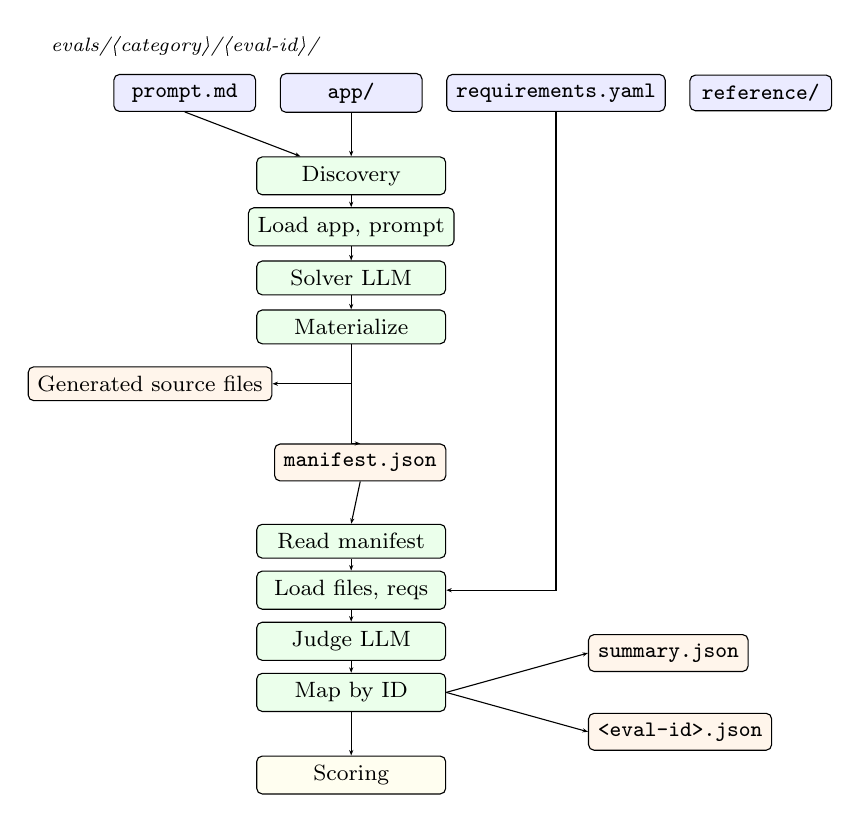
\begin{tikzpicture}[
  data/.style={rectangle, draw, rounded corners=2pt, minimum width=1.8cm, align=center, font=\footnotesize, fill=blue!8},
  process/.style={rectangle, draw, rounded corners=2pt, minimum width=2.4cm, align=center, font=\footnotesize, fill=green!8},
  output/.style={rectangle, draw, rounded corners=2pt, minimum width=1.8cm, align=center, font=\footnotesize, fill=orange!8},
  arrow/.style={-{Stealth[length=2pt]}}
]
  % Row 1: Dataset
  \node[data] (prompt) {\texttt{prompt.md}};
  \node[data, anchor=west] (app) at ([xshift=0.3cm]prompt.east) {\texttt{app/}};
  \node[data, anchor=west] (reqs) at ([xshift=0.3cm]app.east) {\texttt{requirements.yaml}};
  \node[data, anchor=west] (ref) at ([xshift=0.3cm]reqs.east) {\texttt{reference/}};

  % Row 2: Generation CLI
  \node[process] (discover) at ([yshift=-0.8cm]app.south) {Discovery};
  \node[process] (loadgen) at ([yshift=-0.4cm]discover.south) {Load app, prompt};
  \node[process] (solver) at ([yshift=-0.4cm]loadgen.south) {Solver LLM};
  \node[process] (materialize) at ([yshift=-0.4cm]solver.south) {Materialize};

  \draw[arrow] (prompt.south) -- (discover);
  \draw[arrow] (app.south) -- (discover);
  \draw[arrow] (discover) -- (loadgen);
  \draw[arrow] (loadgen) -- (solver);
  \draw[arrow] (solver) -- (materialize);

  % Generation outputs (row centered between materialize and read manifest)
  \node[output, anchor=east] (genfiles) at ([xshift=-1cm, yshift=-0.5cm]materialize.south) {Generated source files};
  \node[output, anchor=east] (manifest) at ([xshift=1.21cm, yshift=-1.5cm]materialize.south) {\texttt{manifest.json}};
  \draw[arrow] (materialize.south) |- (genfiles.east);
  \draw[arrow] (materialize.south) |- (manifest.north);

  % Row 3: Judge CLI
  \node[process] (readmanifest) at ([yshift=-2.5cm]materialize.south) {Read manifest};
  \node[process] (loadjudge) at ([yshift=-0.4cm]readmanifest.south) {Load files, reqs};
  \node[process] (judge) at ([yshift=-0.4cm]loadjudge.south) {Judge LLM};
  \node[process] (mapreq) at ([yshift=-0.4cm]judge.south) {Map by ID};

  \draw[arrow] (manifest.south) -- (readmanifest.north);
  \draw[arrow] (reqs.south) |- (loadjudge.east);
  \draw[arrow] (readmanifest) -- (loadjudge);
  \draw[arrow] (loadjudge) -- (judge);
  \draw[arrow] (judge) -- (mapreq);

  % Judge outputs
  \node[output, anchor=west] (summary) at ([xshift=1.8cm, yshift=0.5cm]mapreq.east) {\texttt{summary.json}};
  \node[output, anchor=west] (pereval) at ([xshift=1.8cm, yshift=-0.5cm]mapreq.east) {\texttt{<eval-id>.json}};
  \draw[arrow] (mapreq.east) -- (summary.west);
  \draw[arrow] (mapreq.east) -- (pereval.west);

  % Row 4: Scoring
  \node[process, fill=yellow!6] (scoring) at ([yshift=-0.8cm]mapreq.south) {Scoring};
  \draw[arrow] (mapreq) -- (scoring);

  % Dataset label
  \node[font=\scriptsize\itshape, anchor=south] at ([yshift=0.1cm]prompt.north) {evals/\textlangle category\textrangle/\textlangle eval-id\textrangle/};
\end{tikzpicture}
\caption{End-to-end pipeline of the React Native Evals benchmark. Dataset inputs (blue) feed the Generation CLI (described in \cref{sec:generation}), producing \texttt{manifest.json} and source files generated by the solver. The Judge CLI (described in \cref{sec:judgement}) reads the manifest and \texttt{requirements.yaml}, runs the judge LLM, maps verdicts by requirement ID, and writes \texttt{summary.json} along with telemetry data. Scoring computes metrics as described in \cref{sec:scoring}.}
\label{fig:pipeline-flow}
\end{figure}

\subsection{Generation stage inputs}
\label{sec:generation}

\begin{enumerate}
  \item \textbf{Discovery}: discover evals
  \item \textbf{Load \texttt{app/}}: read solution template (files on which the solver performs the task) and copy it to a temporary directory, in which the solver LLM will operate
  \item \textbf{Load \texttt{prompt.md}}: parse the task definition, run solver model, write generated files and \\\texttt{manifest.json} to the configured output directory.
\end{enumerate}

\subsubsection{\texttt{prompt.md}}

Task prompt used by the solver model. A representative logical template of this type of file is presented in \cref{lst:promptmd-template}.

\begin{listing}[h]
\begin{tcolorbox}[colback=gray!20,  % light gray background
                  colframe=gray!60, % border color
                  rounded corners,   % rounded edges
                  boxrule=0.5mm,    % border thickness
                  left=4mm, right=4mm, top=2mm, bottom=2mm, % padding
                  title=\texttt{prompt.md} example]    % optional title
Implement X where performing interaction Y causes Z and state A uses an animation B from package C.
\end{tcolorbox}
\caption{Example structure of a prompt in the benchmark.}
\label{lst:promptmd-template}
\end{listing}

\subsubsection{\texttt{app/}}

The \texttt{app/} directory must contain all files serving as baseline input provided to the solver. The files that shall be evaluated by the judge must be listed in the \texttt{requirements.yaml} file.

\subsection{Judgement stage inputs}
\label{sec:judgement}

Reads eval entries from the generation output and runs an LLM to assess the completion of requirements (specified in \cref{sec:judgement-reqs}) in the generated solution.

\subsubsection{\texttt{manifest.json}}

The manifest file contains a summary of the generation stage (\cref{sec:generation}), containing information according to \cref{lst:manifest-json}.

\begin{listing}[h]
\begin{tcolorbox}[colback=gray!20,  % light gray background
                  colframe=gray!60, % border color
                  rounded corners,   % rounded edges
                  boxrule=0.5mm,    % border thickness
                  left=4mm, right=4mm, top=2mm, bottom=2mm, % padding
                  title=\texttt{requirements.yaml} contract]    % optional title
\begin{minted}[breaklines]{json}
{
  "runId": "YYYY-MM-DDTHH-MM-SS-SSSZ",
  "startedAt": "YYYY-MM-DDTHH:MM:SS.SSSZ",
  "finishedAt": "YYYY-MM-DDTHH:MM:SS.SSSZ",
  "solverModel": "<MODEL_NAME>",
  "pattern": "evals/**/*",
  "evalCount": 1,
  "evalsProcessed": 1,
  "evalsErrored": 0,
  "evals": [
    {
      "evalId": "01-category-task",
      "evalPath": "evals/category/task",
      "outputFiles": [
        "App.tsx",
        "styles.ts"
      ],
      "generatedPath": "category/task"
    }
  ]
}
\end{minted}
\end{tcolorbox}
\caption{The contract of \texttt{manifest.json} file, an artifact of the generation stage.}
\label{lst:manifest-json}
\end{listing}

\subsubsection{\texttt{requirements.yaml}}
\label{sec:judgement-reqs}

Task prompt used by the solver model. A representative logical template of this type of file is presented in \cref{lst:requirements-yaml-template}.
The \mintinline{yaml}{version} is a constant element present for compatibility reasons for future versions of the project, that must be set to \mintinline{yaml}{1}.
The \mintinline{yaml}{inputs} list shall contain all files to be copied to the temporary workspace for the solver.
The \mintinline{yaml}{requirements} list shall contain all the requirements, described in natural language. The requirements should explicitly state specific elements or behaviors that the presence of is to be asserted in the judgement stage.
Optionally, each requirement may contain a \mintinline{yaml}{weight} value set to a positive value to emphasize its impact on the score for that requirement. If omitted, its value defaults to \mintinline{yaml}{1}.

\begin{listing}[h]
\begin{tcolorbox}[colback=gray!20,  % light gray background
                  colframe=gray!60, % border color
                  rounded corners,   % rounded edges
                  boxrule=0.5mm,    % border thickness
                  left=4mm, right=4mm, top=2mm, bottom=2mm, % padding
                  title=\texttt{requirements.yaml} contract]    % optional title
\begin{minted}[breaklines]{yaml}
version: 1
inputs:
  files:
    - app/App.tsx
    - app/styles.ts
requirements:
  - id: implementation-use-X-api
    description: Must use API `X` from package `A`.
    weight: 1
  - id: implementation-avoid-Y-api
    description: Must NOT use deprecated API `Y` from package `A`.
    weight: 1
  - id: toggle-state-on-click
    description: Upon click on button `B`, the visual active state of element `C` must toggle.
    weight: 1
\end{minted}
\end{tcolorbox}
\caption{The contract of \texttt{requirements.yaml} file.}
\label{lst:requirements-yaml-template}
\end{listing}

\subsection{OpenCode integration in the judgment stage.}
Execution layer used to call all solver and judge models through one interface (model IDs in the form \texttt{provider/model}, e.g., \texttt{openai/gpt-5.3-codex}). Before judging starts, the runner ensures that a local OpenCode server is available on the configured port; if a server is already running, it is reused. For each eval, the Judge CLI creates a new OpenCode session, sends the constructed judge prompt, and requests schema-constrained structured output. If strict structured output fails, a JSON fallback path is used and validated before scoring.

After each judge call, the pipeline can fetch OpenCode session metadata (conversation, token usage, and file-diff summary) and store it as \texttt{<eval-id>.opencode-session.judge.json}. Standard judge outputs are written incrementally as \texttt{runs/<input-folder>/evals/<eval-id>.json}, and the run-level aggregate is written as \texttt{summary.json}. Judging runs with bounded concurrency and retry logic; when \texttt{--fail-fast} is disabled, failed evals do not stop the run and are counted in \texttt{evalsErrored}.

The runner supports bounded concurrency. If an eval fails and \texttt{----fail-fast} is not enabled, the run continues and the eval is counted in \texttt{evalsErrored}.

The judge CLI also supports targeted re-judging over existing judge outputs using \\\texttt{----rerun-requirements-file} with \texttt{----output}; optionally pass \texttt{----rerun-requirement-id} to refresh only one requirement. Without \texttt{----rerun-requirement-id}, all requirements for the targeted eval are re-judged and replaced in the per-eval JSON. It also supports \texttt{----rerun-missing-judgements} with \texttt{----output} to scan for and judge all evals missing per-eval judge JSON outputs (the same missing rows counted by \texttt{evalsErrored} in the rebuilt summary). In rerun modes, the previous \texttt{summary.json} is backed up as \texttt{summary.backup.<timestamp>.json}, and a new aggregate summary is generated from the current per-eval result set.

\section{Solver Stage Methodology}

The solver methodology treats each benchmark item as a constrained code-generation task: the model receives a task prompt plus project context, produces a complete implementation artifact, and is evaluated only against task-defined requirements. The same solver protocol is applied across all tasks and runs, with outputs stored in a structured, reproducible format, ensuring fair comparison across models and direct traceability between generated code and downstream requirement-level scores.

\subsection{Input Construction}
The solver is given:
\begin{itemize}
  \item the eval prompt from \texttt{prompt.md}
  \item the baseline files from \texttt{app/}
  \item a fixed system instruction requiring the model to return all provided files with modifications applied
\end{itemize}

The runner formats baseline files into a structured prompt with explicit file tags.

\subsection{Output Contract}
The solver returns structured output with:
\begin{itemize}
  \item \texttt{summary}: short description of performed changes
  \item \texttt{files[]}: array of \texttt{\{path, content\}}
\end{itemize}

Returned paths are sanitized before writing to disk (e.g., stripping leading slashes and removing traversal segments such as \texttt{..}).

\subsection{Model Requirement}
The generation CLI requires \texttt{----model}. When set to \texttt{noop}, the generation stage copies files from each eval's \texttt{reference/} directory into the configured output and still writes a validated \texttt{manifest.json}. Any other model value runs normal solver generation.

\section{LLM Judge Methodology}

For React Native coding tasks, an LLM-based judge is an effective approach that balances benefits with preparation workload. The quality of a task depends on semantic correctness across multiple files and layers. Component logic, state flow, navigation behavior, asynchronous handling, and API usage are all important. Many valid implementations exist, and strict deterministic rules do not apply to the semantic complexity of mobile apps. Deterministic checks are excellent for narrow invariants, but as a standalone judge, they overly penalize acceptable variations, miss errors in higher-level reasoning, and require constant revisions as frameworks and programming patterns evolve. A requirements- or specification-based LLM judge can evaluate requirements at the intent level, detect nuanced errors, incorrect cycle assumptions, or unstable query invalidation logic, and assign consistent, evidence-based results at the requirements level, thus remaining independent of the solver model and style. In practice, this approach provides a better fit to real-world engineering tasks and faster benchmark evolution than pure determinism pipelines for React Native.

\subsection{Requirements Parsing}
\texttt{requirements.yaml} is parsed and validated at runtime. The enforced schema requires:
\begin{itemize}
  \item \texttt{version}: positive integer (defaults to 1 via schema default)
  \item \texttt{requirements[]}: non-empty list of objects with:
  \begin{itemize}
    \item \texttt{id} (non-empty string)
    \item \texttt{description} (non-empty string)
    \item optional positive \texttt{weight}
  \end{itemize}
\end{itemize}

Extra fields are ignored by the current runtime parser.

\subsection{Deterministic \texttt{implementation-} Requirement Convention}
The repository documents an authoring convention for deterministic requirements:
\begin{itemize}
  \item prefix deterministic, source-verifiable requirement IDs with \texttt{implementation-}
  \item use \texttt{weight: 1} by default to avoid overweighting implementation details
\end{itemize}

Examples include required imports, API usage patterns, and specific wiring that can be verified directly from files.

\textbf{Important distinction:} the runner does \emph{not} infer behavior from ID prefixes such as \texttt{implementation-}. Prefixes are an authoring convention; scoring changes only when a requirement explicitly sets \texttt{weight} in \texttt{requirements.yaml}.

\subsection{Technical Eval Authoring Controls}
For technical categories (for example navigation, animation, storage), requirement quality is governed by additional authoring controls documented under \texttt{docs/}.
\begin{itemize}
  \item \textbf{Recent API shift audit:} before requirement writing, review official docs plus recent releases/changelogs for each core library, and extract concrete ``new preferred API'' and ``deprecated/removed API'' signals with dates.
  \item \textbf{Evidence-gated \texttt{MUST NOT}:} use explicit \texttt{MUST NOT} clauses only when backed by primary-source deprecation/removal or correctness caveats.
  \item \textbf{Implementation-level specificity:} technical diversity is measured at \\requirement/API-constraint level, not prompt wording level.
  \item \textbf{Similarity budget:} within a library subgroup, keep shared baseline requirements small (target: at most two shared IDs) and maintain multiple eval-specific implementation constraints per eval.
  \item \textbf{Judge input scope:} set \texttt{inputs.files} to implementation files under evaluation (for example \texttt{app/App.tsx}) rather than prompt-only artifacts.
\end{itemize}

These controls are authoring policy for dataset quality; they are not independently enforced by runner schema validation.

\subsection{Judge Prompt Construction}
The judge prompt includes:
\begin{itemize}
  \item declared requirements (including weights when present)
  \item generated files under evaluation
  \item rules instructing the judge to use only provided files as evidence and return one result per declared requirement ID
\end{itemize}

\subsection{Structured Judge Output}
The judge returns structured output with:
\begin{itemize}
  \item optional \texttt{summary}
  \item \texttt{requirements[]}, where each row includes \texttt{id}, \texttt{passed}, \texttt{reason}, \texttt{evidence[]}, and optional \texttt{confidence}
\end{itemize}

\subsection{Requirement Mapping and Failure Policy}
Judge rows are mapped back to declared requirements by ID.
\begin{itemize}
  \item If a declared requirement is missing from judge output, the runner marks it as failed.
  \item The runner emits a fixed failure reason indicating that the judge did not return a result for that requirement.
  \item Extra judge rows for undeclared IDs are ignored for scoring.
  \item Requirement weights are normalized before scoring (Section~\ref{sec:scoring}).
\end{itemize}

The judge CLI requires \texttt{----model}; there is no judge skip/noop path.

\section{Scoring Methodology}
\label{sec:scoring}

Each model is evaluated through the identical benchmark pipeline in 10 independent runs to reduce variance from stochastic generation and judging effects and to produce a statistically more reliable performance estimate. In every run, the model receives the same task set, prompt protocol, and scoring rules, while random factors may still lead to different outputs and per-task scores. Repeating the full pipeline therefore captures both central tendency and dispersion of performance, allowing analysis to rely on aggregated results (e.g., mean and spread) rather than a potentially noisy single-run outcome. This design improves fairness in cross-model comparison and supports more robust conclusions about relative capability on React Native tasks.

\subsection{Requirement Weight Normalization}
Each requirement weight is normalized as:
\[
w_i' =
\begin{cases}
w_i & \text{if } w_i \text{ is finite and } w_i > 0 \\
1 & \text{otherwise}
\end{cases}
\]

This normalization is defensive. In normal operation, the runtime schema already requires positive weights when provided.

\subsection{Per-Eval Weighted Requirement Score}
For an eval with declared requirements \(R\), normalized weights \(w_i'\), and binary pass indicators \(p_i\):
\[
\text{totalWeight} = \sum_{i \in R} w_i'
\]
\[
\text{passedWeight} = \sum_{i \in R} p_i \cdot w_i'
\]
\[
\text{scoreRatio} =
\begin{cases}
0 & \text{if } \text{totalWeight} = 0 \\
\frac{\text{passedWeight}}{\text{totalWeight}} & \text{otherwise}
\end{cases}
\]

The runner rounds \texttt{passedWeight}, \texttt{totalWeight}, and \texttt{scoreRatio} to 4 decimal places.

\textbf{Interpretation example.} If requirements have weights \([2, 2, 1]\) and pass outcomes \([1, 0, 1]\), then the per-eval score is:
\[
\frac{2 + 0 + 1}{2 + 2 + 1} = \frac{3}{5} = 0.6
\]
This pattern is relevant only when authors intentionally assign non-default weights to specific requirements.

\subsection{Run-Level Aggregate Score}
Let \(E^+\) be the set of evals that complete successfully (i.e., without an unrecovered pipeline error). The summary field \texttt{weightedAverageScore} is:
\[
\texttt{weightedAverageScore} =
\begin{cases}
0 & \text{if } |E^+| = 0 \\
\frac{1}{|E^+|}\sum_{e \in E^+}\texttt{scoreRatio}_e & \text{otherwise}
\end{cases}
\]
rounded to 4 decimal places.

\textbf{Interpretation note:} the ``weighted'' part refers to weights within each eval. The run-level average itself is an unweighted mean across successful evals.

\subsection{Additional Summary Metrics}
The run summary also reports:
\begin{itemize}
  \item \texttt{requirementsTotal}
  \item \texttt{requirementsPassed}
  \item \texttt{evalsErrored}
\end{itemize}

For successful evals, each row includes \texttt{requirementsTotal}, \texttt{requirementsPassed},
and \texttt{scoreRatio}. For pipeline errors, each row includes \texttt{status=error}
along with the eval identifier and path.

\section{Artifacts and Output Schema}
Each run writes artifacts to deterministic generation and judge directories:
\begin{itemize}
  \item \texttt{runs/<input-folder>/evals/<eval-id>.json}: per-eval judge results (written as each eval completes)
  \item \texttt{runs/<input-folder>/summary.json}: aggregate judge summary (written at end)
  \item generated artifacts and \texttt{manifest.json}: written by generation CLI to a user-selected output directory (default: \texttt{generated/<model>-<run-id>})
  \item per-eval OpenCode session snapshots:
  \begin{itemize}
    \item generation: \texttt{<generated-eval-dir>/opencode-session.solver.json}
    \item judging: \texttt{runs/<input-folder>/evals/<eval-id>.opencode-session.judge.json}
  \end{itemize}
  \item optional debug artifacts when \texttt{----debug} is enabled
\end{itemize}

Per-eval results include solver and judge model identifiers, mapped requirement verdicts, per-eval score, generated file list, and optional \texttt{judgeSessionArtifactPath} when session capture succeeds. The generation \texttt{manifest.json} includes \texttt{solverSessionArtifactPath} for each processed eval.

\section{Repeat Orchestration Script}
The repository provides \texttt{scripts/bench-series.sh} to run multiple full cycles (generation + judging) for variance analysis. Configure via environment variables:
\begin{itemize}
  \item \texttt{RUN\_COUNT}: number of run+judge iterations (default: 10)
  \item \texttt{BENCH\_RUN\_ARGS}: arguments for the generation CLI (e.g.\ \texttt{----model}, \texttt{----pattern})
  \item \texttt{BENCH\_JUDGE\_ARGS}: arguments for the judge CLI (e.g.\ \texttt{----model}); \texttt{----input} is injected per run
  \item \texttt{BENCH\_OUTPUT\_BASE}: base directory for outputs (default: \texttt{/tmp/bench-seriess})
\end{itemize}

For each of the \texttt{RUN\_COUNT} iterations, the script runs generation then judging. If either step fails, it retries up to 3 times before failing the script. Outputs are written to \\\texttt{<BENCH\_OUTPUT\_BASE>/<timestamp>/run-1}, \texttt{run-2}, etc.

\section{Results}

\Cref{fig:model-comparison} summarizes both overall and category-level performance across twelve solver models. In overall weighted average score, \texttt{claude-opus-4.6} leads (84.4\%), followed by \texttt{gpt-5.3-codex} (80.9\%) and \texttt{gemini-3.1-pro-preview} (78.9\%), while \texttt{deepseek-r1-distill-qwen-32b} records the lowest score (31.8\%). The category breakdown is non-uniform: navigation is generally the strongest category for most models, whereas animation and async-state are more discriminative and better separate mid-tier and lower-tier performance. For each model, detailed analysis is provided in Appendix~A. \Cref{tab:tokens-by-model} summarizes token usage by model.


\begin{figure}[htbp]
\centering
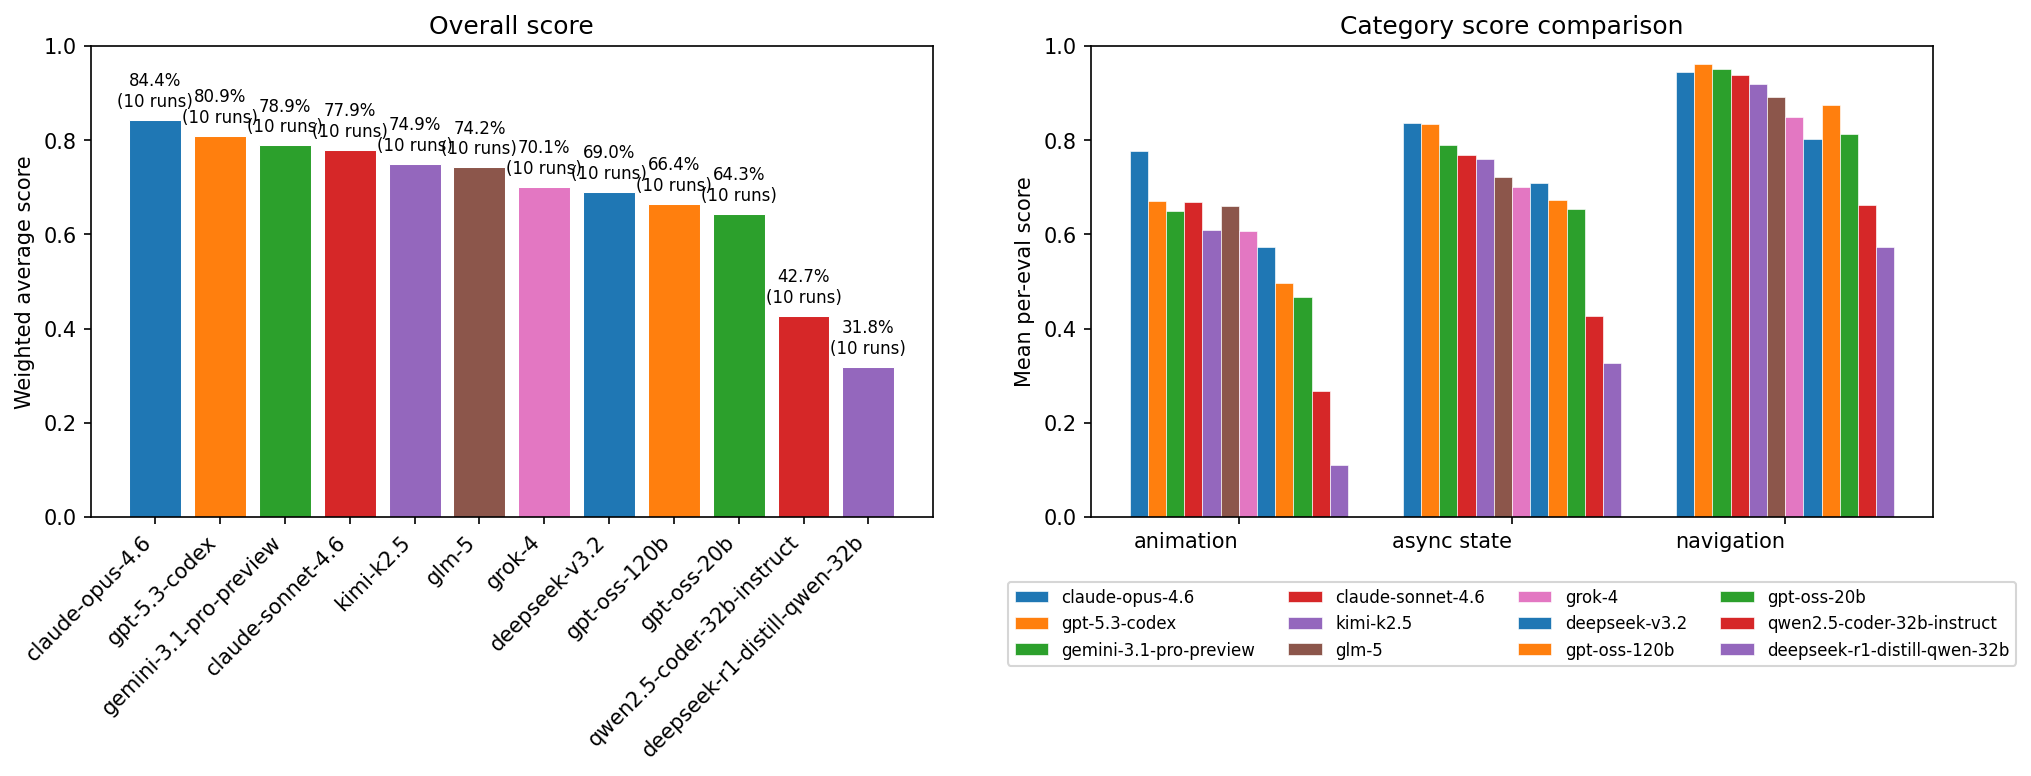
\includegraphics[width=\textwidth]{export/comparison_plot.png}
\caption{Overall score and category comparison across all models.}
\label{fig:model-comparison}
\end{figure}

\begin{table}[htbp]
\centering
\small
\begin{tabular}{r l c c}
\toprule
\textbf{Rank} & \textbf{Model} & \textbf{Weighted average score} & \textbf{Runs} \\
\midrule
1  & claude-opus-4.6                & 0.844 (84.4\%) & 10 \\
2  & gpt-5.3-codex                  & 0.809 (80.9\%) & 10 \\
3  & gemini-3.1-pro-preview         & 0.789 (78.9\%) & 10 \\
4  & claude-sonnet-4.6              & 0.779 (77.9\%) & 10 \\
5  & kimi-k2.5                      & 0.749 (74.9\%) & 10 \\
6  & glm-5                          & 0.742 (74.2\%) & 10 \\
7  & grok-4                         & 0.701 (70.1\%) & 10 \\
8  & deepseek-v3.2                  & 0.690 (69.0\%) & 10 \\
9  & gpt-oss-120b                   & 0.664 (66.4\%) & 10 \\
10 & gpt-oss-20b                    & 0.643 (64.3\%) & 10 \\
11 & qwen2.5-coder-32b-instruct     & 0.427 (42.7\%) & 10 \\
12 & deepseek-r1-distill-qwen-32b   & 0.318 (31.8\%) & 10 \\
\bottomrule
\end{tabular}
\caption{Overall model comparison from packed result archives.}
\label{tab:model-comparison-overall}
\end{table}

% Requires: \usepackage{booktabs}
\begin{table}[htbp]
\centering
\begin{tabular}{lrr}
\toprule
Model & Tokens mean & Tokens stddev \\
\midrule
claude-opus-4.6 & 885,374 & 1,537 \\
claude-opus-4.7 & 1,209,561 & 723 \\
claude-sonnet-4.6 & 885,424 & 1090 \\
composer-2 & --- & --- \\
composer-2-fast & --- & --- \\
deepseek-r1-distill-qwen-32b & 254,437 & 1,247 \\
deepseek-v3.2 & 5,590,132 & 782,834 \\
gemini-3.1-pro-preview & 1,074,284 & 12,826 \\
gemma-4-31B-it & 885,910 & 91,050 \\
glm-5 & 1,171,183 & 152,778 \\
gpt-5.3-codex & 778,463 & 49,875 \\
gpt-5.4 & 869,589 & 50,085 \\
gpt-oss-120b & 653,327 & 27,343 \\
gpt-oss-20b & 765,263 & 57,402 \\
grok-4 & 1,257,083 & 38,612 \\
kimi-k2.5 & 2,500,716 & 408,562 \\
minimax-m2.7 & 1,261,454 & 131,780 \\
qwen2.5-coder-32b-instruct & 732,531 & 15,154 \\
\bottomrule
\end{tabular}
\caption{Total tokens per run by model. Mean and stddev computed across runs. It was impossible to **precisely** determine Composer 2 and Composer 2 Fast values for the runs.}
\label{tab:tokens-by-model}
\end{table}


The full benchmark pipeline executed successfully end-to-end across the evaluated model set, confirming that the current eval suite is operationally usable for comparative React Native model assessment.

\section{Recommended Reporting Protocol}
For comparative studies, report at minimum:
\begin{enumerate}
  \item repository commit hash (dataset and runner version)
  \item CLI options (\texttt{run: ----pattern, ----model, ----timeout, ----concurrency, ----output}; \\\texttt{judge: ----model, ----timeout, ----concurrency, ----input} \\and optional rerun flags \texttt{----rerun-requirements-file}, \texttt{----output}, \\scope optional \texttt{----rerun-requirement-id}, scope optional \texttt{----rerun-missing-judgements})
  \item execution date and time
  \item counts of discovered, processed, and errored evals
  \item \texttt{weightedAverageScore} and \texttt{requirementsPassed/Total}
  \item generated artifact source directory
\end{enumerate}

Repeat runs are recommended. The \texttt{bench:repeat} script (or \texttt{scripts/bench-series.sh}) automates multiple cycles. The current runner does not explicitly pin a random seed or decoding settings (e.g., temperature) in solver or judge calls, so provider defaults and model nondeterminism can affect results.

\section{Limitations and Threats to Validity}
\begin{itemize}
  \item \textbf{Judge dependence:} requirement verdicts depend on the configured LLM judge model and prompt behavior.
  \item \textbf{Requirement-interpretation ambiguity:} without seeded reference context, ambiguous requirement phrasing can increase variance in judge decisions.
  \item \textbf{Binary requirement outcomes:} there is no partial credit within a single requirement.
  \item \textbf{Run-level averaging choice:} the summary score is unweighted across evals, which can underweight larger evals.
  \item \textbf{Pipeline error exclusion from mean:} errored evals are counted separately and excluded from the run-level score average.
  \item \textbf{Authoring-convention variability:} conventions such as \texttt{implementation} improve consistency but are not enforced by the runtime parser.
\end{itemize}

\section{Acknowledgments}

Text drafting and editorial refinement used artificial intelligence-assisted tooling. All technical claims, implementation details, equations, and reported metrics were manually verified against repository code and captured experiment artifacts before inclusion.

\section{Conflict of Interest}

The authors are affiliated with Callstack. The experiments used commercially available infrastructure acquired and operated independently; no direct sponsorship, funding, or editorial influence was provided for this work.

\section{Conclusion}
We evaluated \textbf{12} solver models on the React Native eval suite (\textbf{43} evals in total), with \textbf{10 repeated runs per model} under the same pipeline and scoring rules. Across completed runs, the highest mean \texttt{weightedAverageScore} was \textbf{0.844} (\textbf{84.4\%}, model: \texttt{claude-opus-4.6}); the median across models was \textbf{0.722} (\textbf{72.2\%}). Category-level analysis (Figure~\ref{fig:model-comparison}) shows strongest performance on \textbf{navigation} and weakest performance on \textbf{animation}, with \textbf{async state} in between and strongly differentiating mid-tier models. Recurring failures were concentrated in behavior-heavy requirements, especially animation dynamics and async-state consistency/invalidation logic.

Two practical implications follow. First, React Native development difficulty is not uniform: models that are competitive on navigation and structural code generation can still be unreliable on behavior-heavy work, where correctness depends on timing, gesture/animation dynamics, and state invalidation semantics. For practitioners, this suggests applying the most scrutiny (and the most automated protection via tests and runtime validation) to animation and async-state code paths, even when a model performs strongly overall. Second, requirement-level evaluation yields actionable signals: per-requirement verdict traces support targeted prompt iteration, scaffolding improvements, and dataset evolution without collapsing all behavior into a single task-level pass/fail.

From an operational standpoint, token usage varied substantially across models (Table~\ref{tab:tokens-by-model}), ranging from \textbf{116,581} mean tokens per run (\texttt{claude-sonnet-4.6}) to \textbf{821,708} (\texttt{grok-4}). This highlights a cost/latency frontier that is not directly implied by score alone, and reinforces that model selection for production assistance should consider both category-specific performance and consumption characteristics.

Overall, these results indicate that React Native Evals separates model capability in a reproducible and auditable way while preserving requirement-level interpretability (via explicit per-requirement weights and per-eval verdict artifacts). They also highlight a need to extend the current evaluation set beyond the existing categories to more of the day-to-day React Native surface area, such as handling network requests (including error handling, retries, caching, and cancellation), building custom native integrations, repairing or extending faulty code in partially-correct codebases, keeping pace with the latest versions and breaking changes of common third-party libraries, and more. Future work should also explore judge-robust scoring (e.g., multi-judge consensus and calibrated partial credit) to reduce dependence on any single evaluator while maintaining transparency.


% % Appendix: tables and figures only. No prose.
% Include from parent: % Appendix: tables and figures only. No prose.
% Include from parent: % Appendix: tables and figures only. No prose.
% Include from parent: \input{export/appendix} (compile from repo root)

\appendix
\section{Detailed Results}

\subsection{claude-opus-4.6}

% Table: summary
\input{export/tables/claude-opus-4.6_summary}

% Table: category_summary
\input{export/tables/claude-opus-4.6_category_summary}

% Table: per_eval
\input{export/tables/claude-opus-4.6_per_eval}

\begin{figure}[htbp]
\centering
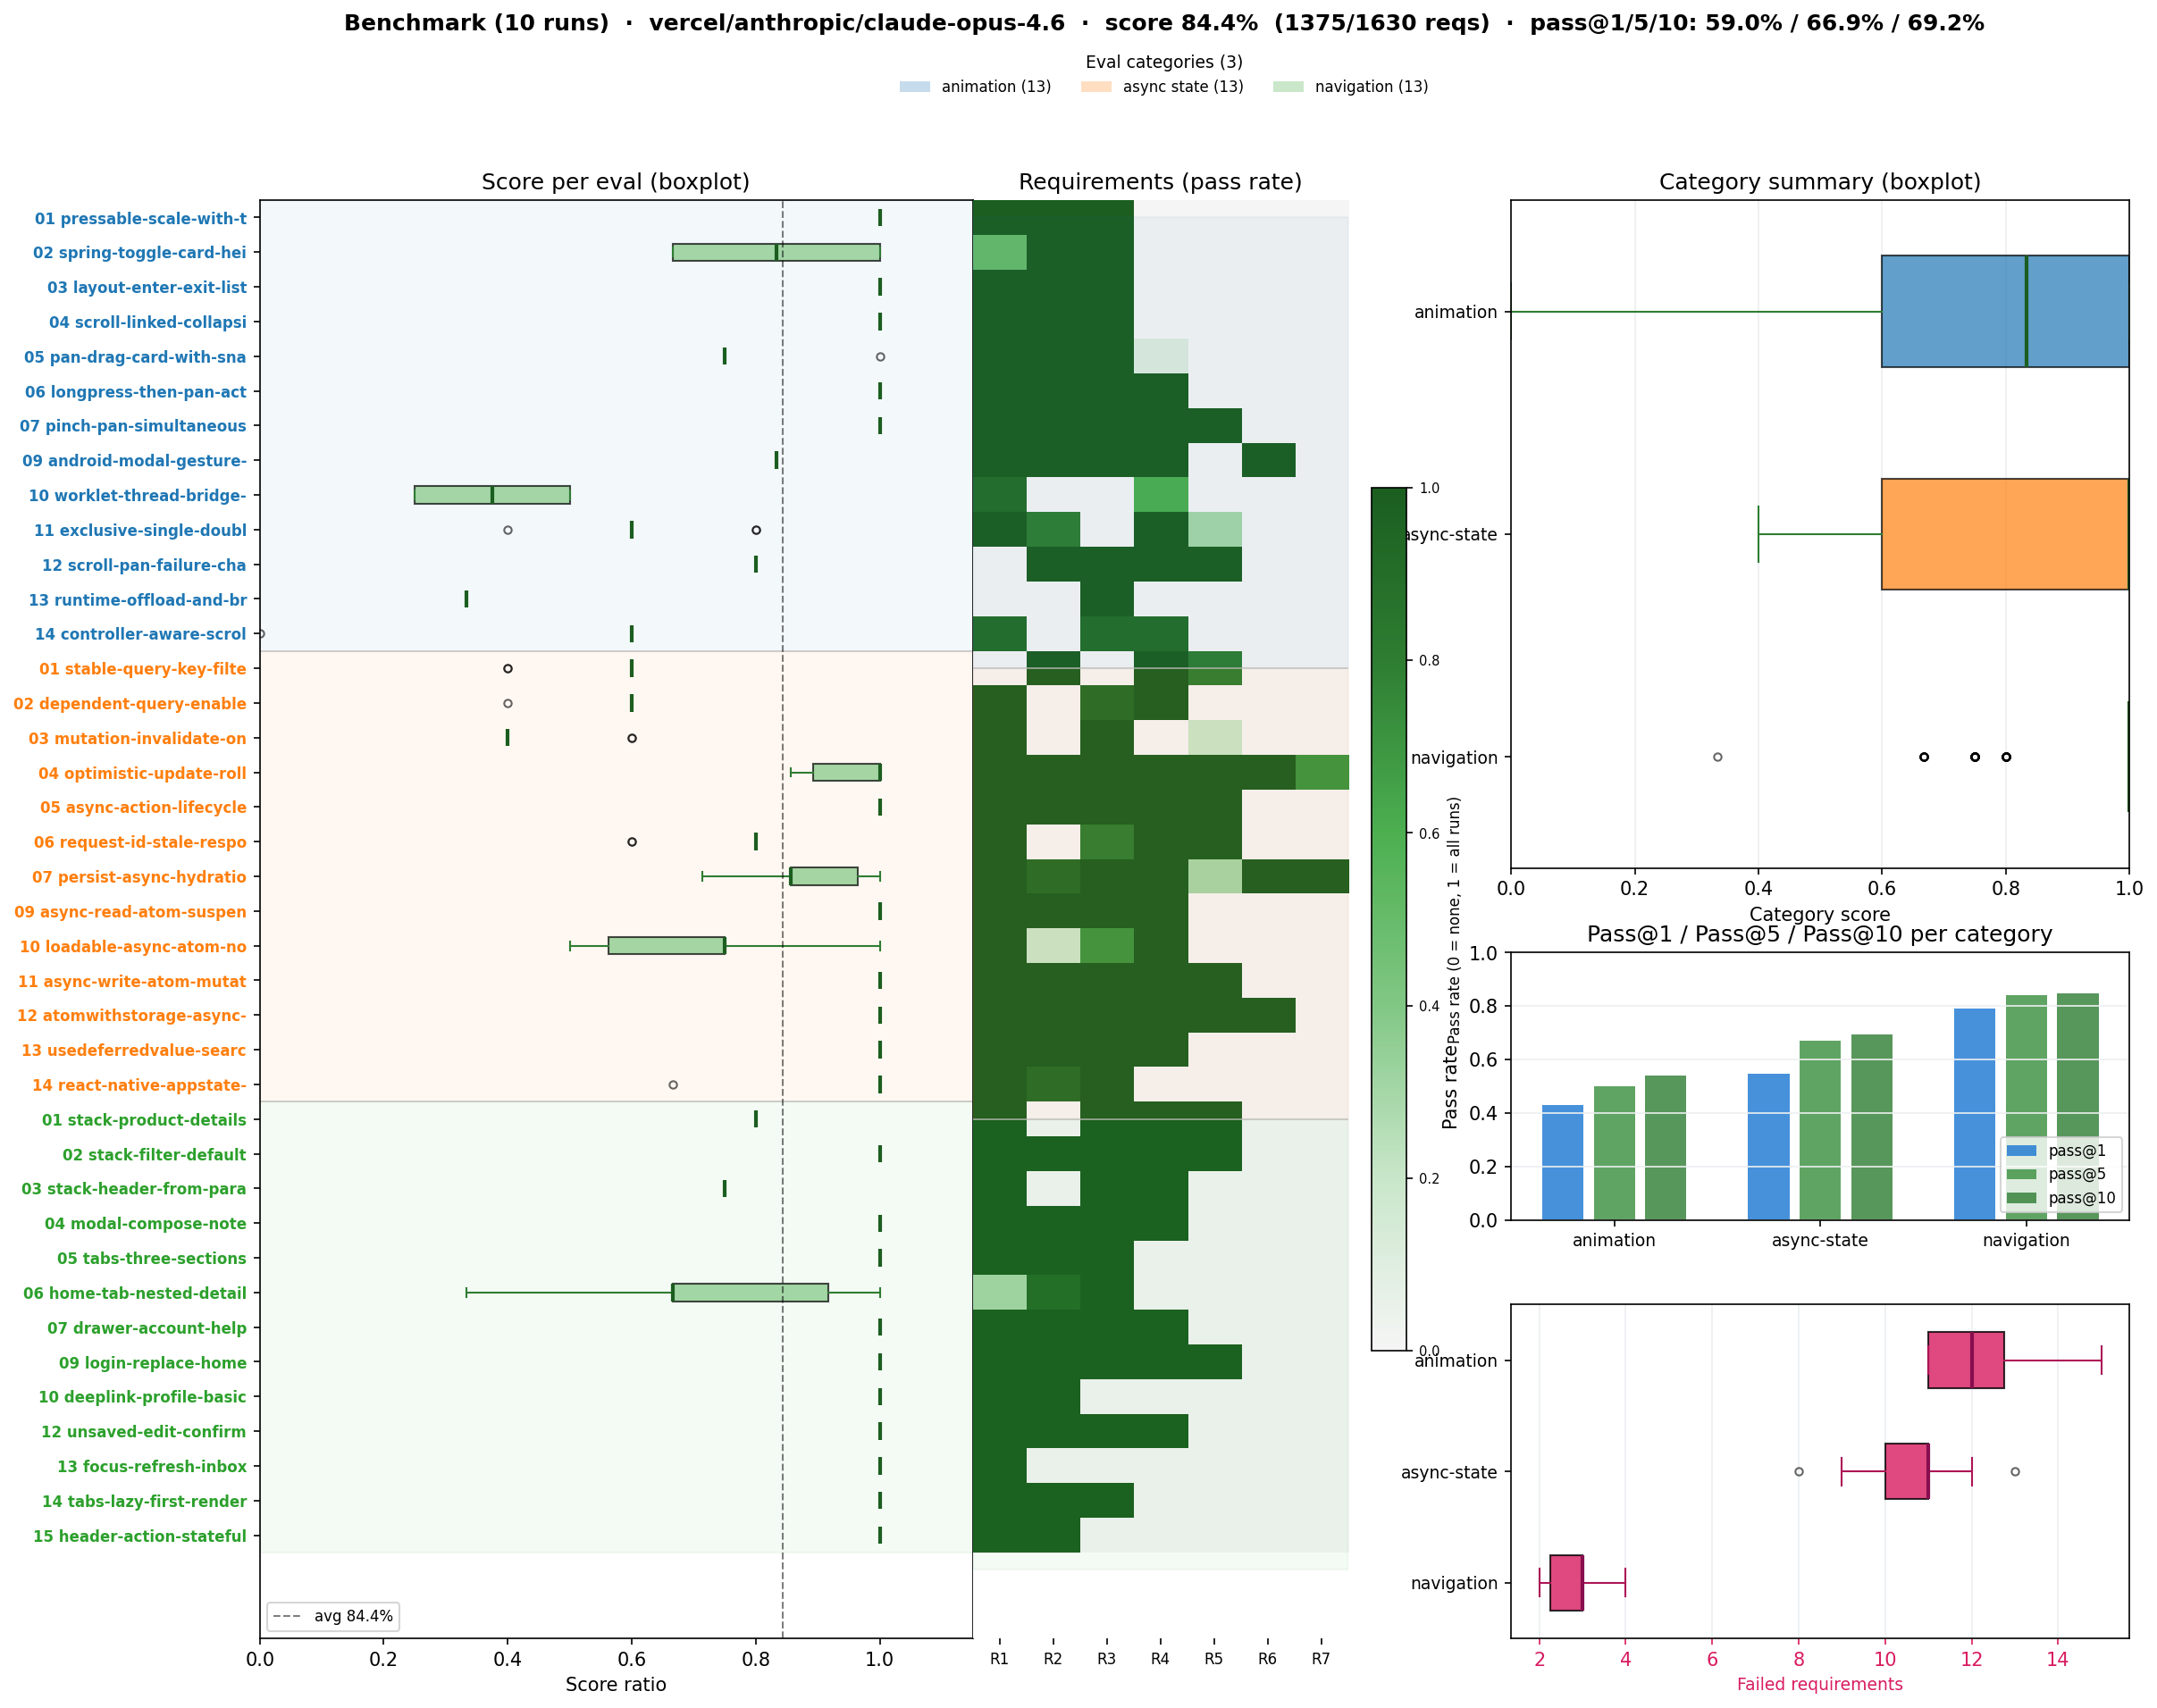
\includegraphics[width=\textwidth]{export/figures/claude-opus-4.6_benchmark_plot.png}
\caption{Benchmark Plot for claude-opus-4.6.}
\end{figure}

\begin{figure}[htbp]
\centering
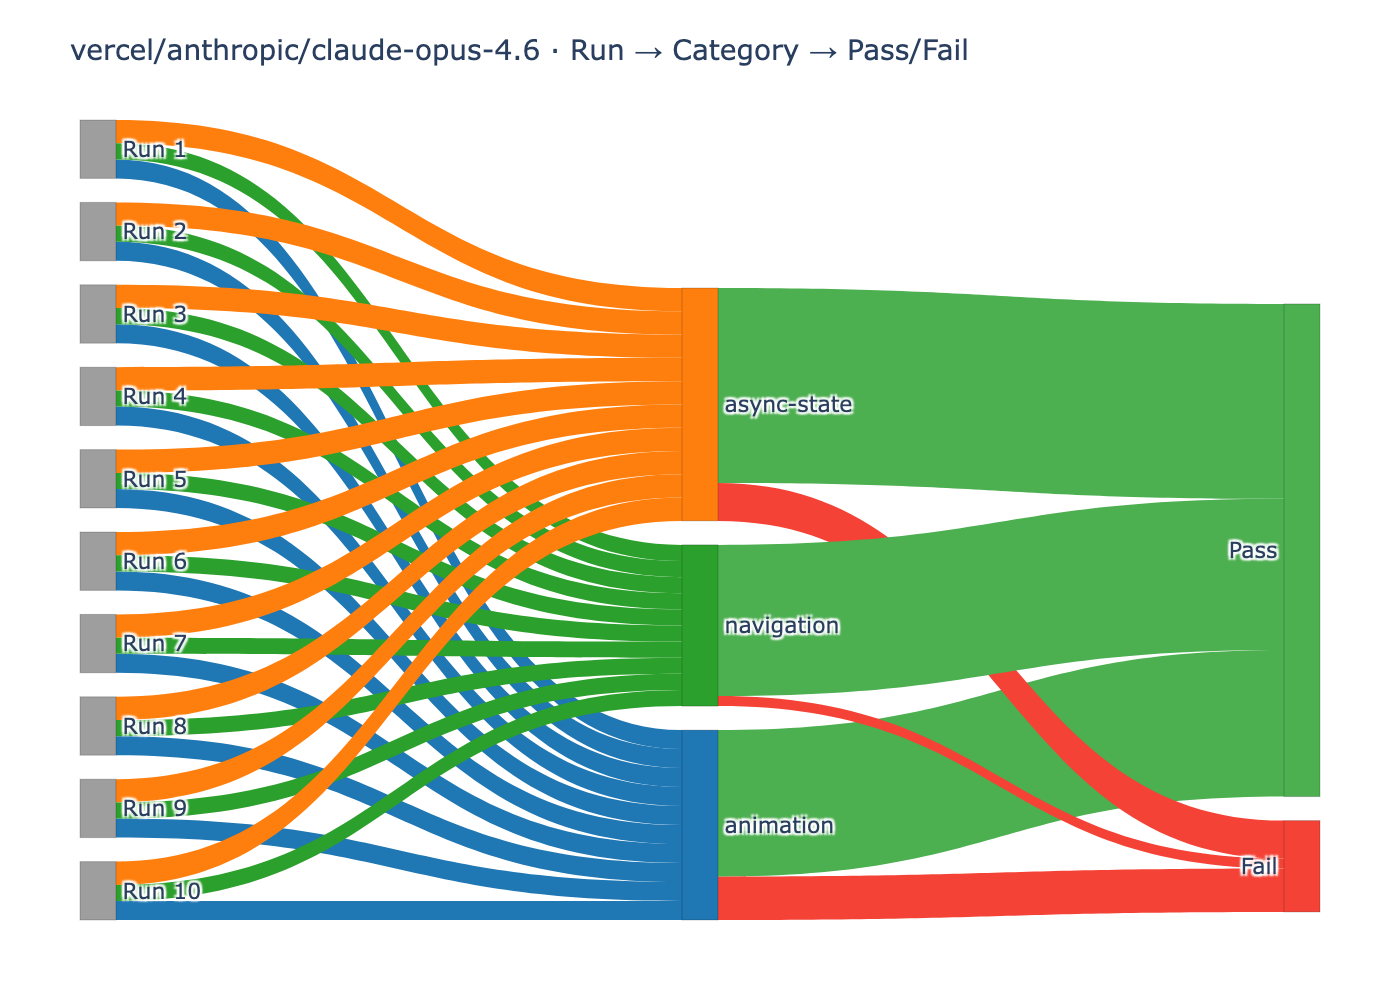
\includegraphics[width=\textwidth]{export/figures/claude-opus-4.6_sankey_per_run.png}
\caption{Sankey per run for claude-opus-4.6 showing the distribution of evals with respect to categories and results}
\end{figure}


\clearpage

\subsection{claude-sonnet-4.6}

% Table: summary
\input{export/tables/claude-sonnet-4.6_summary}

% Table: category_summary
\input{export/tables/claude-sonnet-4.6_category_summary}

% Table: per_eval
\input{export/tables/claude-sonnet-4.6_per_eval}

\begin{figure}[htbp]
\centering
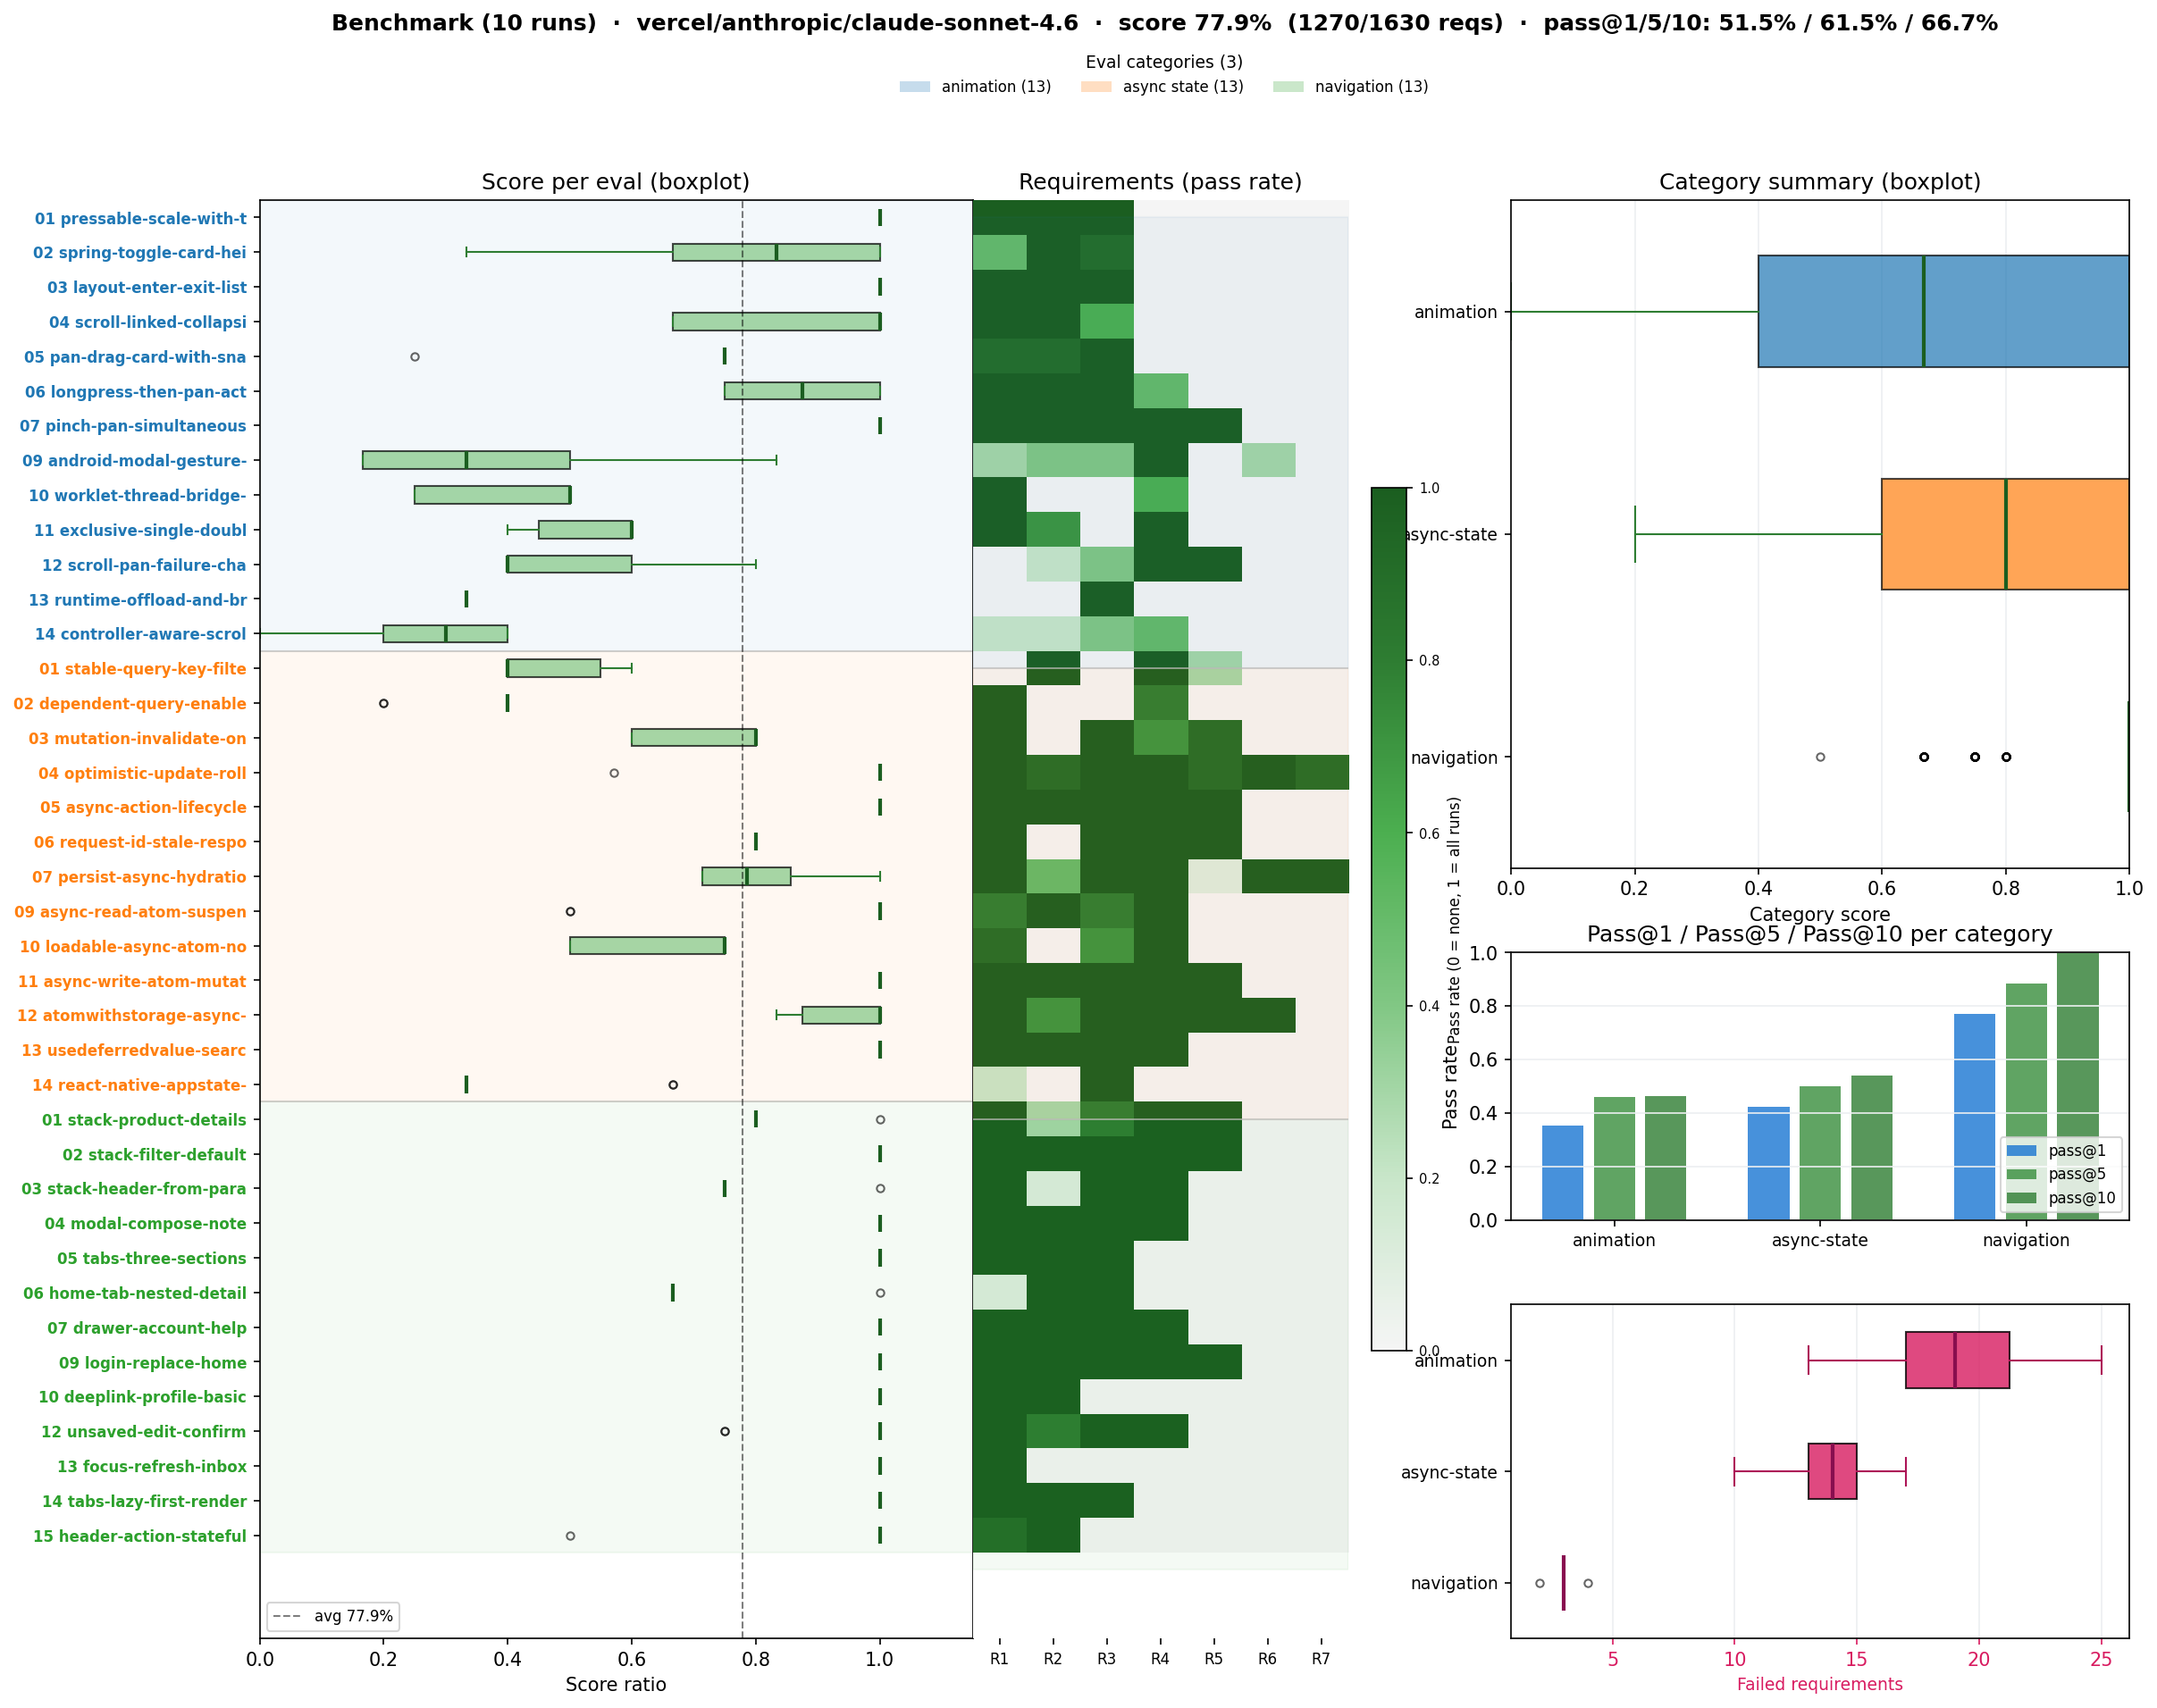
\includegraphics[width=\textwidth]{export/figures/claude-sonnet-4.6_benchmark_plot.png}
\caption{Benchmark Plot for claude-sonnet-4.6.}
\end{figure}

\begin{figure}[htbp]
\centering
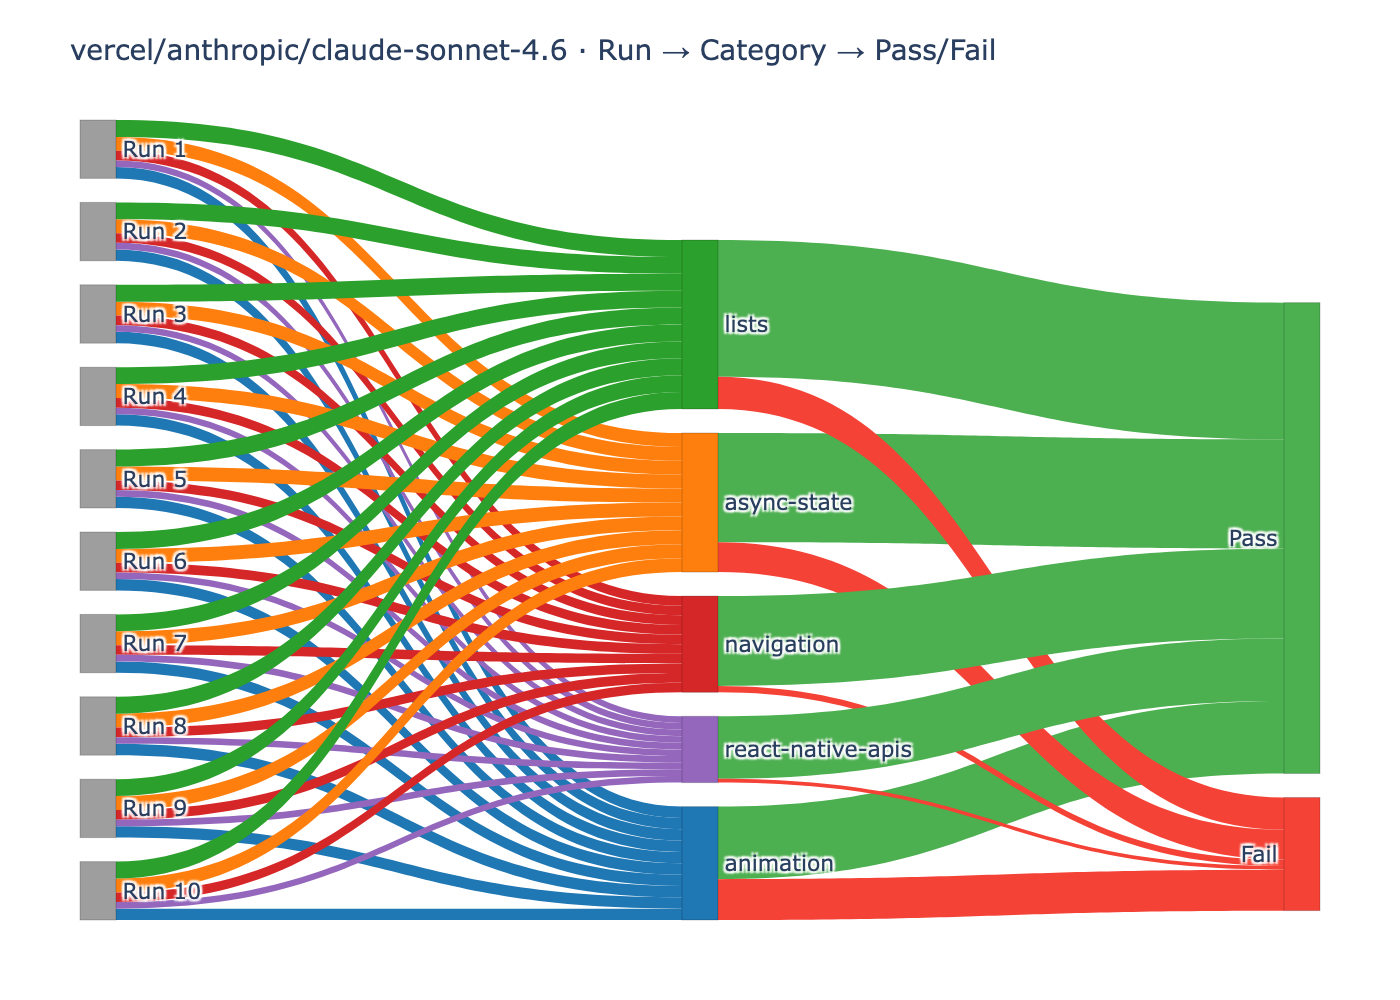
\includegraphics[width=\textwidth]{export/figures/claude-sonnet-4.6_sankey_per_run.png}
\caption{Sankey per run for claude-sonnet-4.6 showing the distribution of evals with respect to categories and results}
\end{figure}


\clearpage

\subsection{deepseek-r1-distill-qwen-32b}

% Table: summary
\input{export/tables/deepseek-r1-distill-qwen-32b_summary}

% Table: category_summary
\input{export/tables/deepseek-r1-distill-qwen-32b_category_summary}

% Table: per_eval
\input{export/tables/deepseek-r1-distill-qwen-32b_per_eval}

\begin{figure}[htbp]
\centering
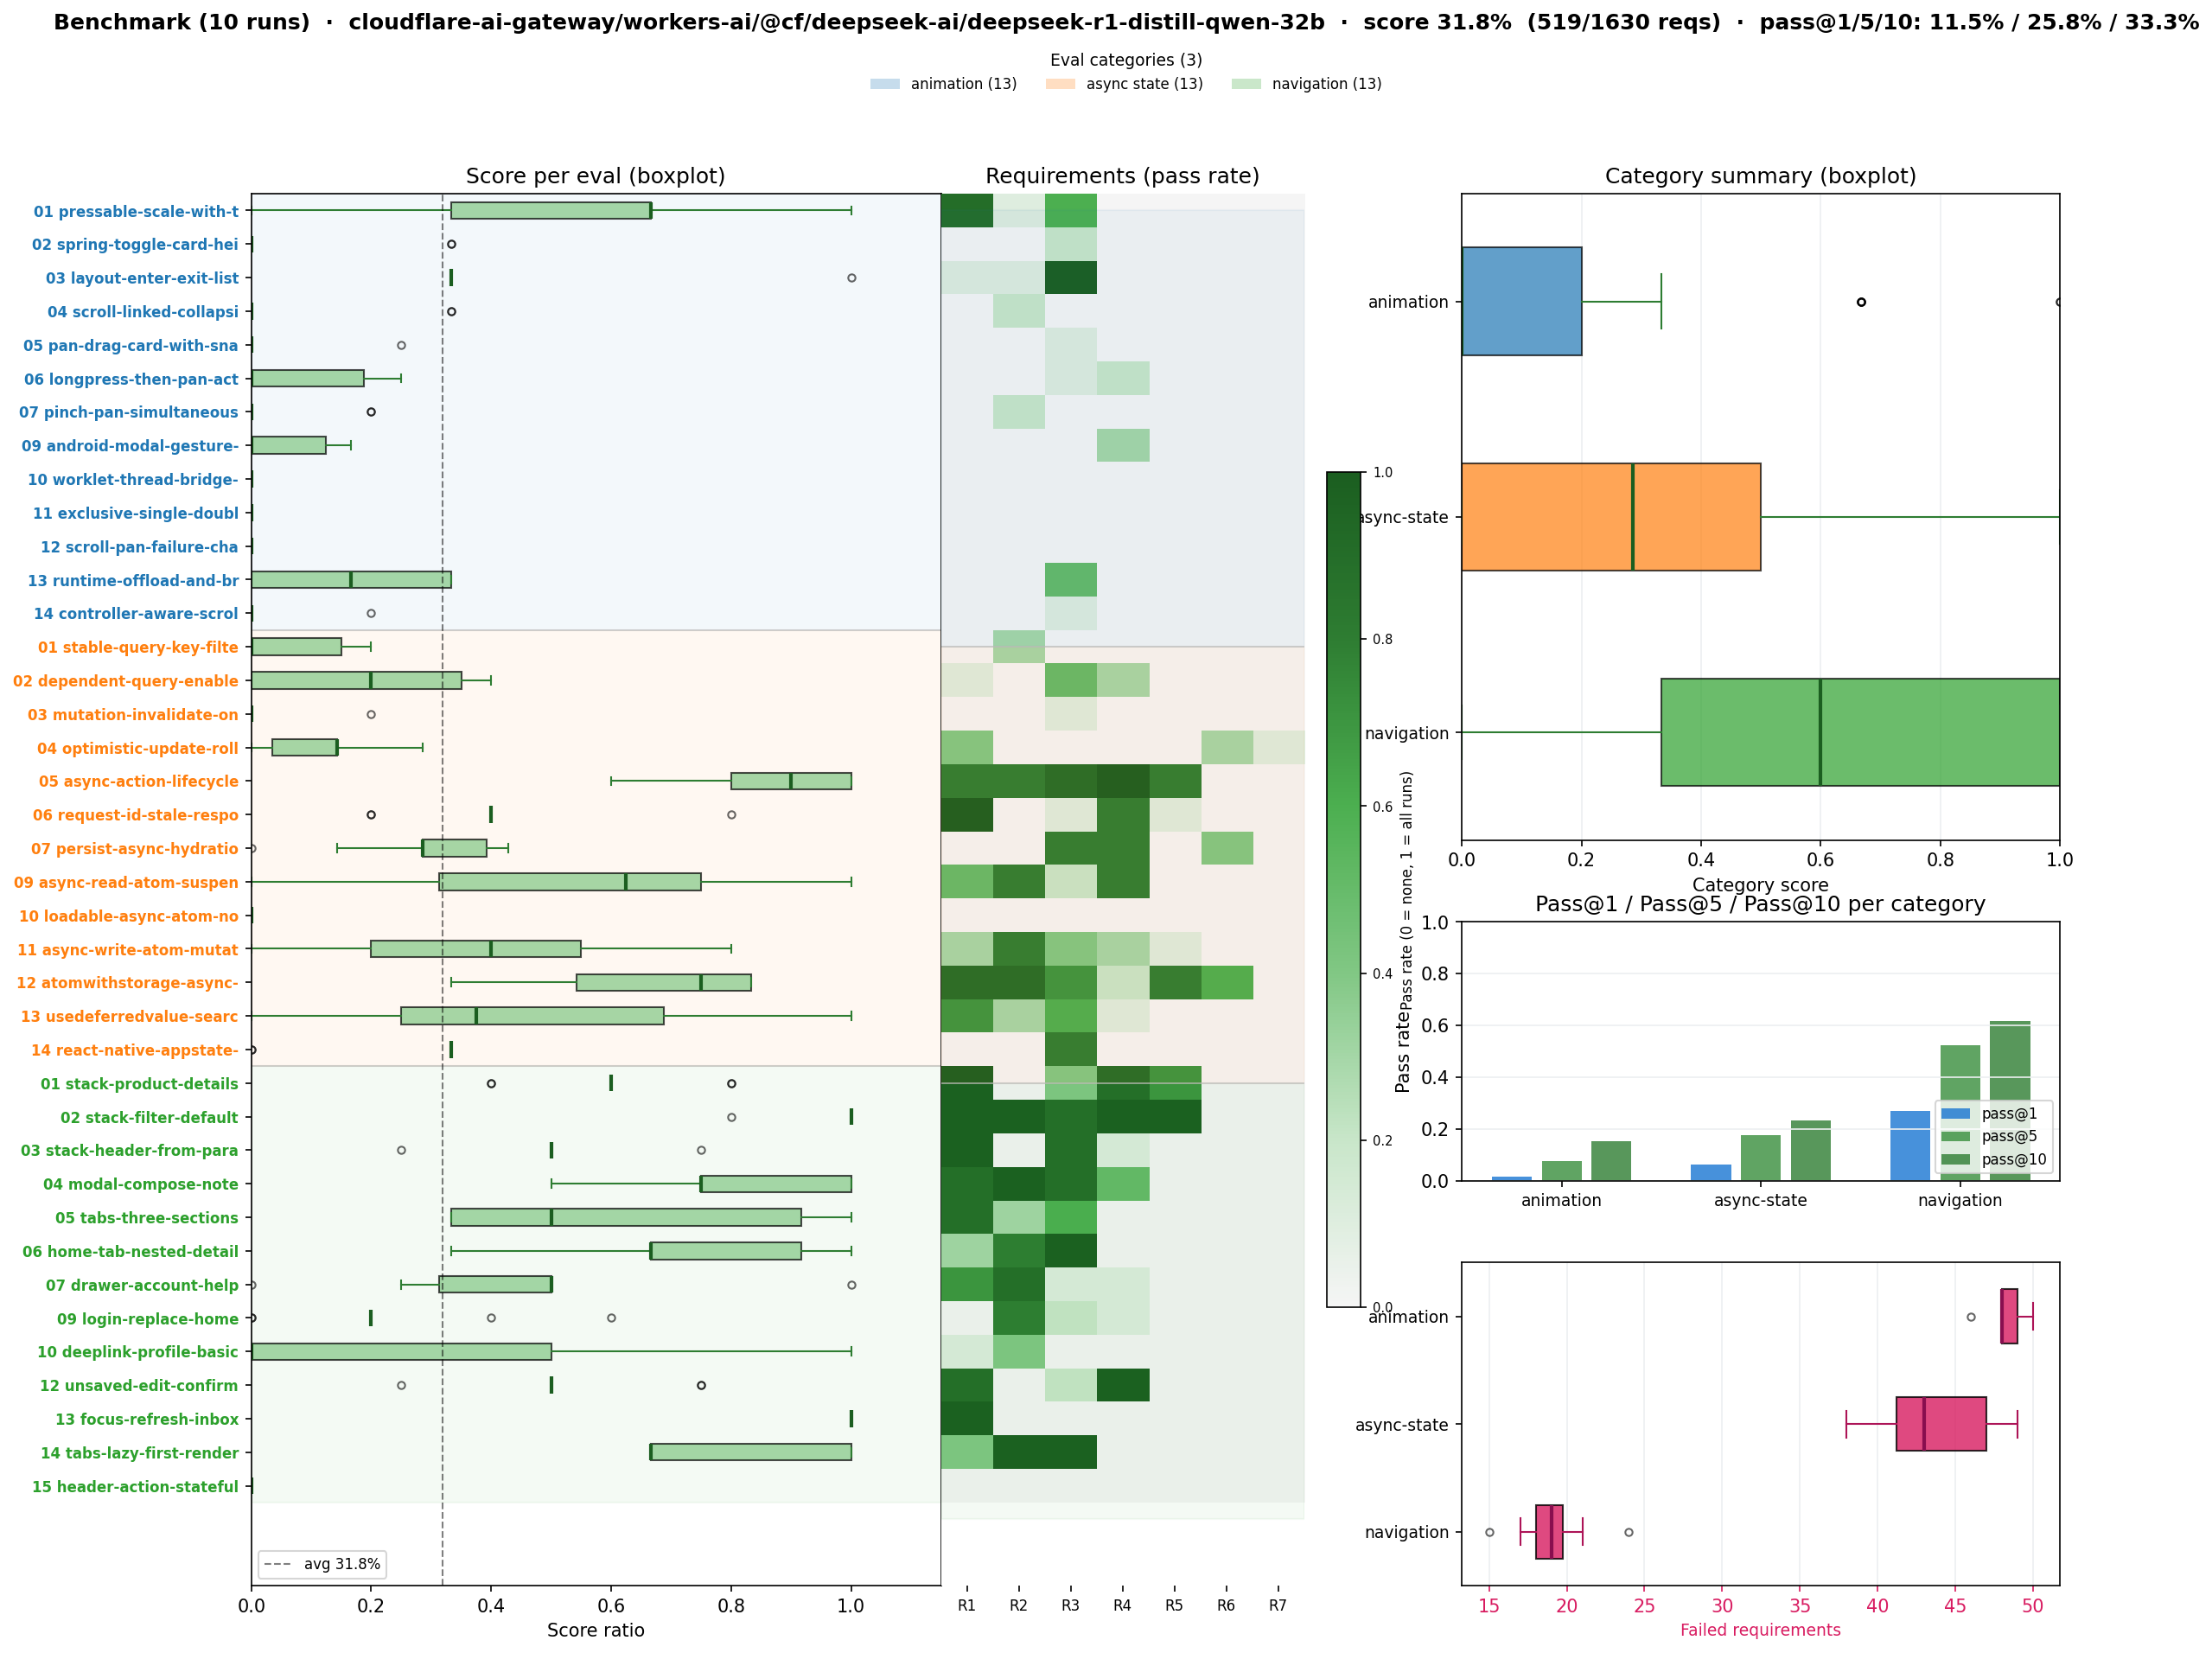
\includegraphics[width=\textwidth]{export/figures/deepseek-r1-distill-qwen-32b_benchmark_plot.png}
\caption{Benchmark Plot for deepseek-r1-distill-qwen-32b.}
\end{figure}

\begin{figure}[htbp]
\centering
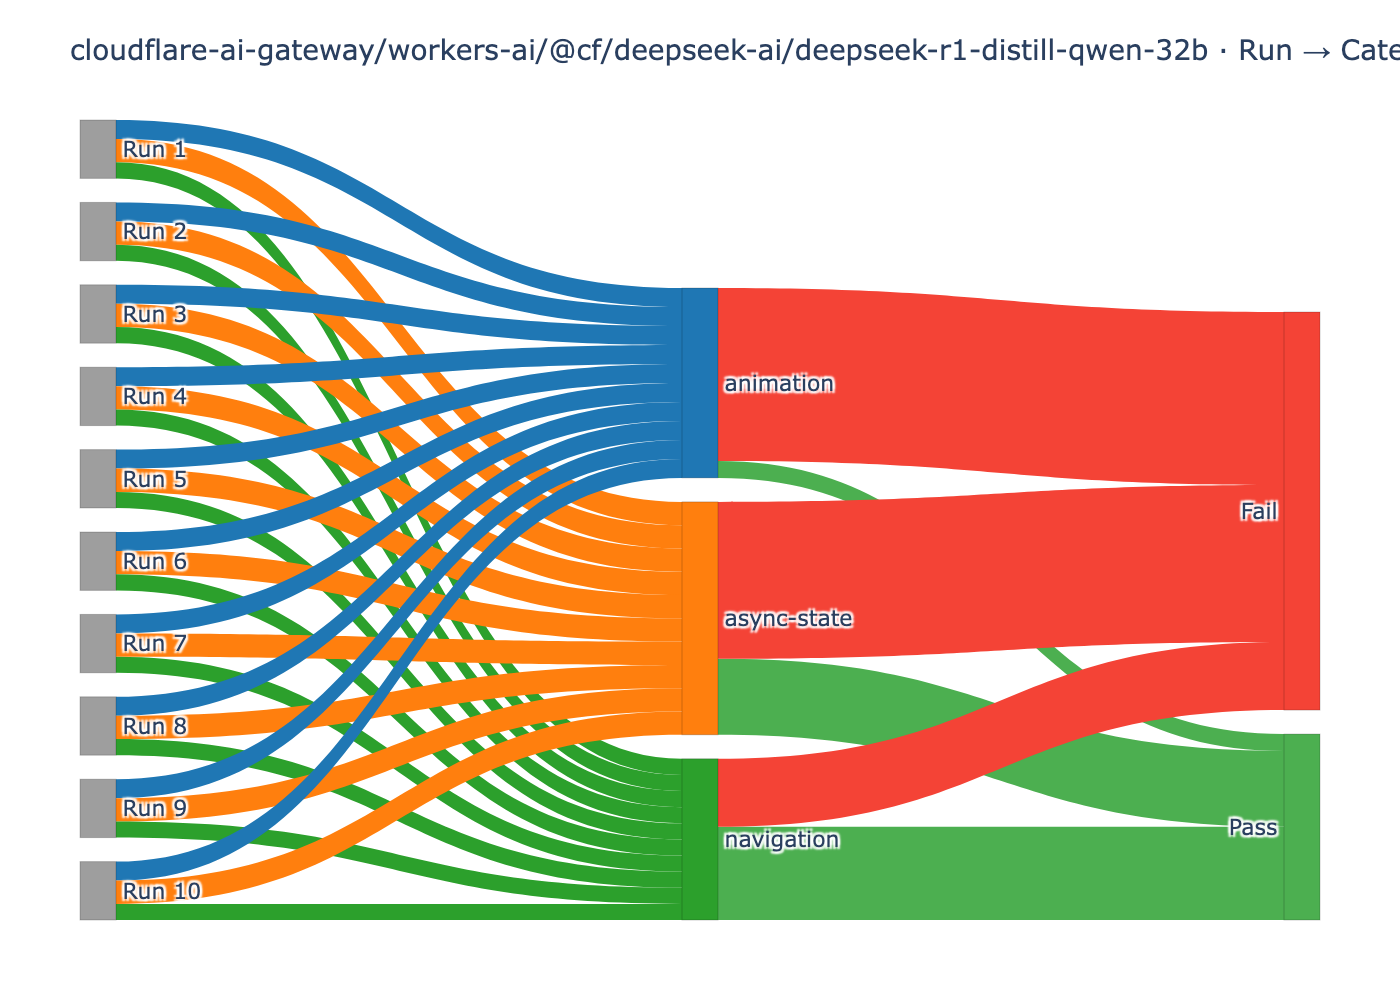
\includegraphics[width=\textwidth]{export/figures/deepseek-r1-distill-qwen-32b_sankey_per_run.png}
\caption{Sankey per run for deepseek-r1-distill-qwen-32b showing the distribution of evals with respect to categories and results}
\end{figure}


\clearpage

\subsection{deepseek-v3.2}

% Table: summary
\input{export/tables/deepseek-v3.2_summary}

% Table: category_summary
\input{export/tables/deepseek-v3.2_category_summary}

% Table: per_eval
\input{export/tables/deepseek-v3.2_per_eval}

\begin{figure}[htbp]
\centering
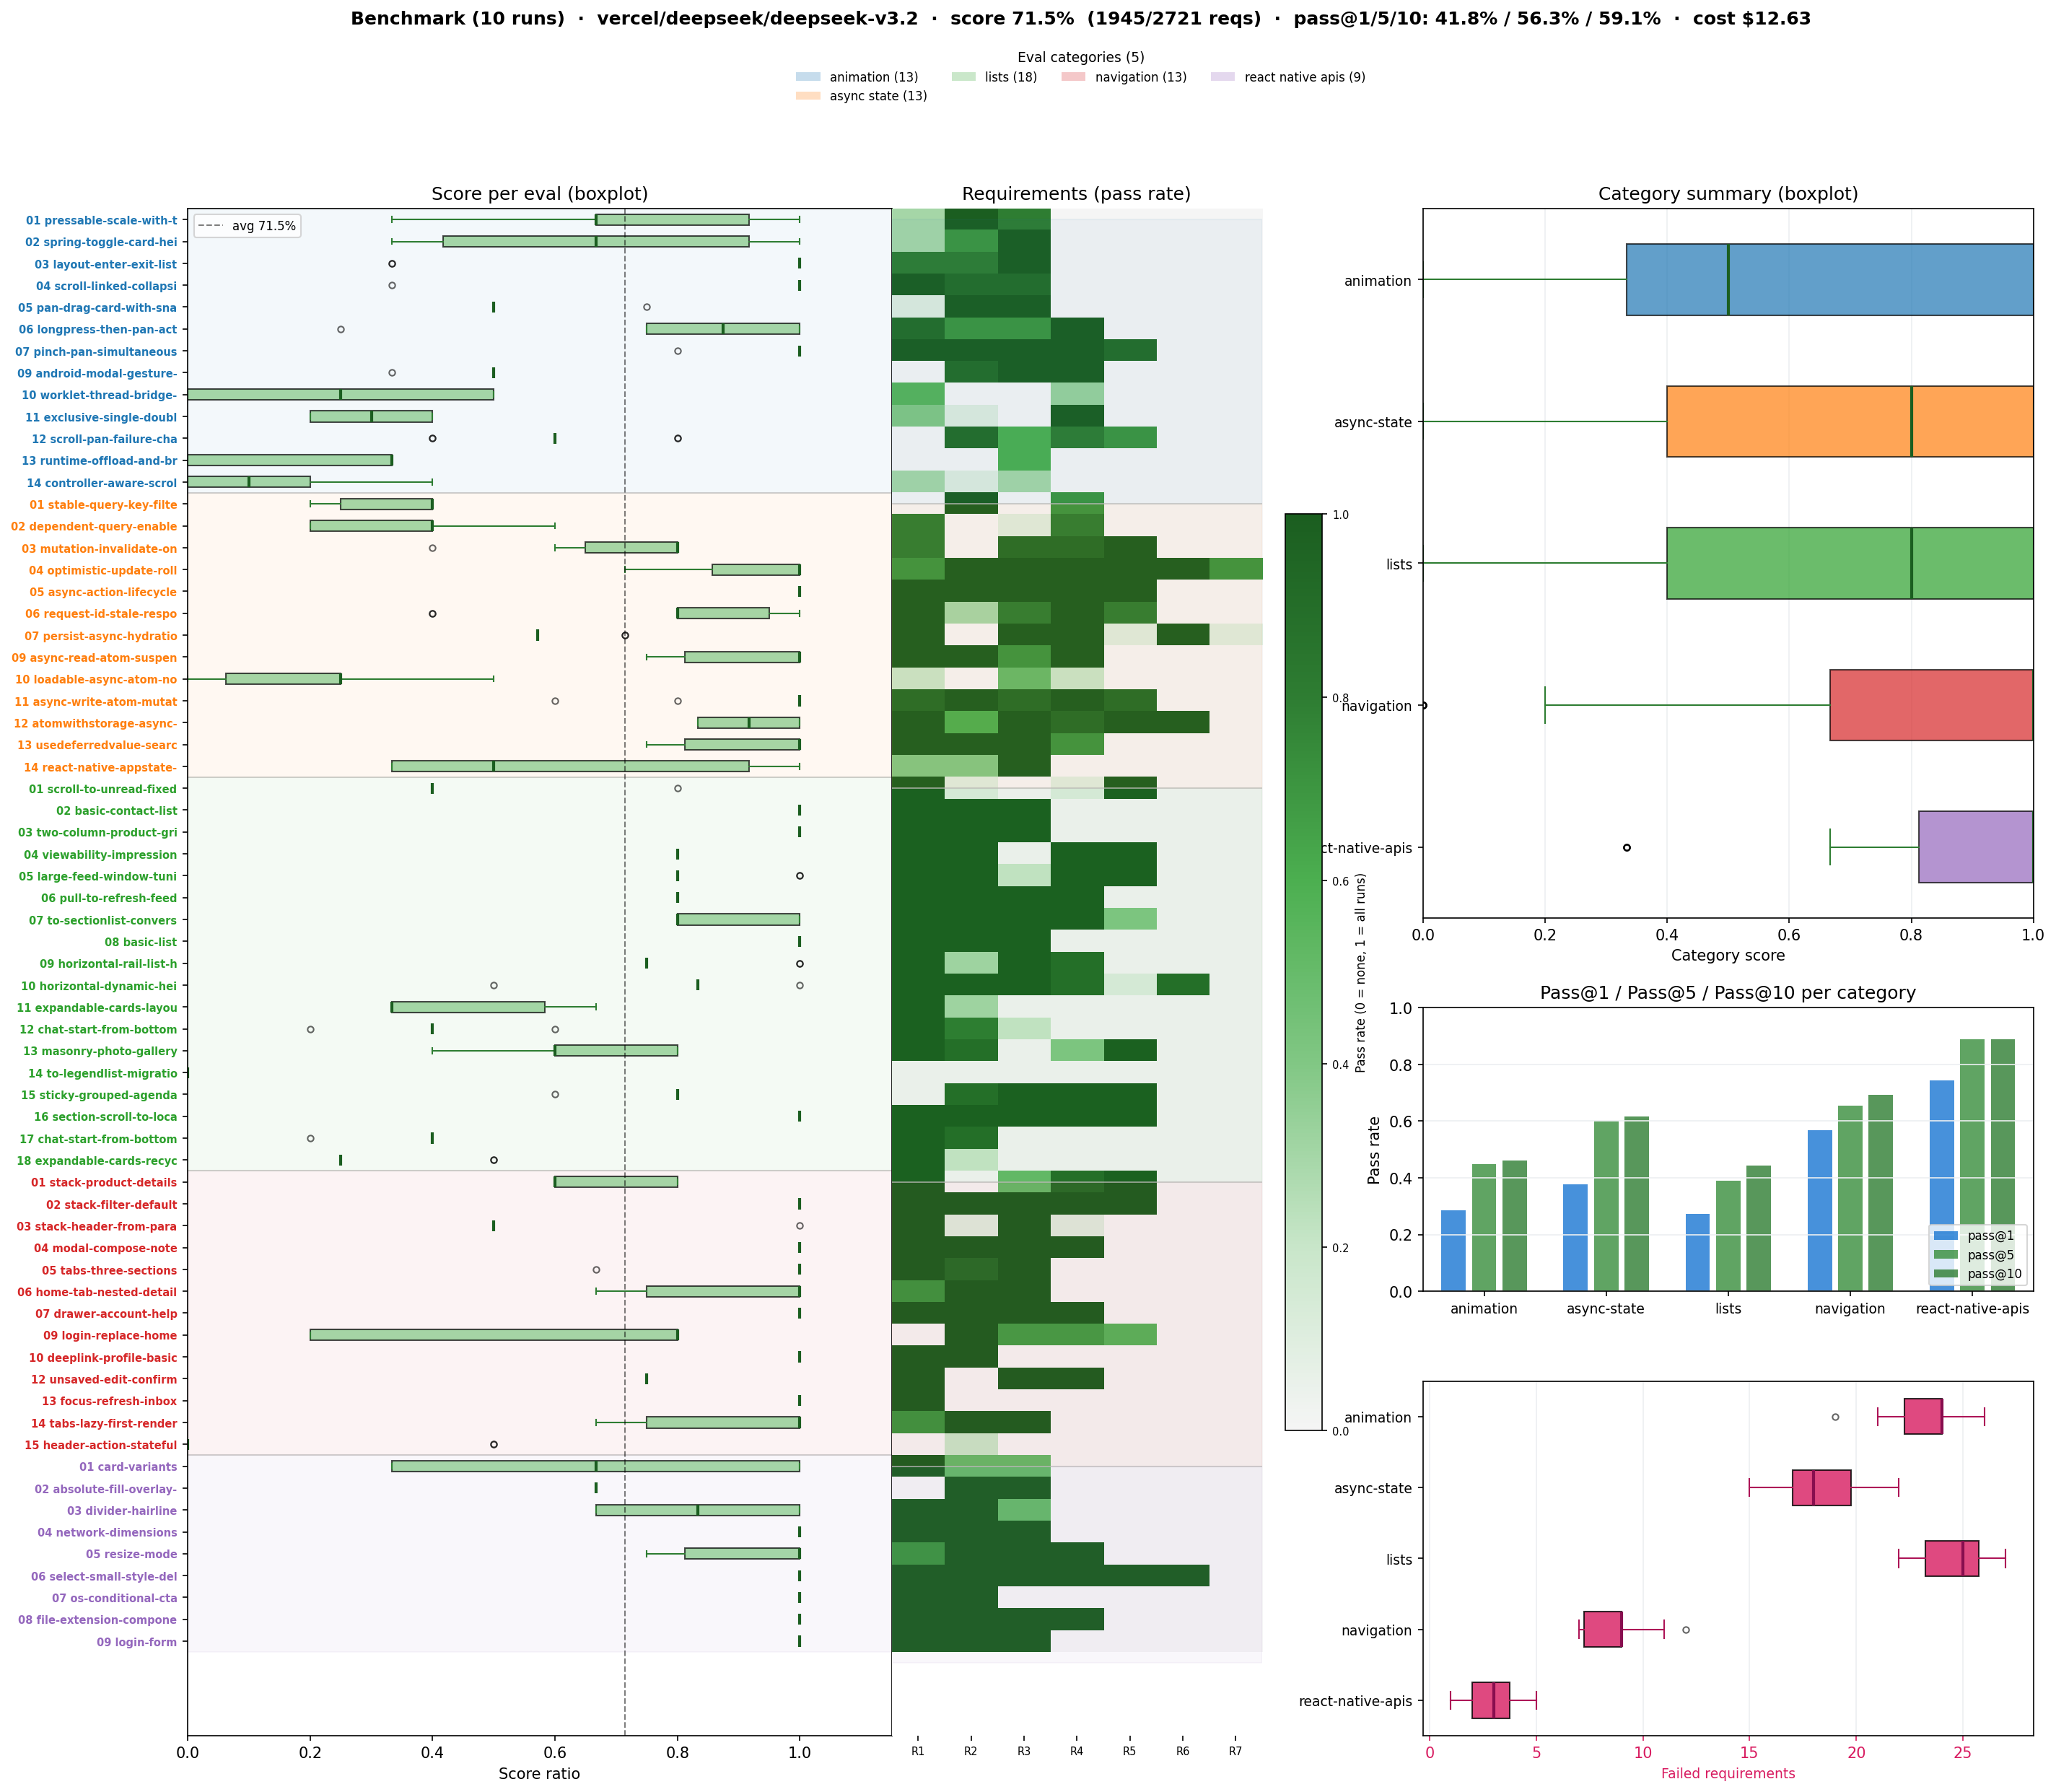
\includegraphics[width=\textwidth]{export/figures/deepseek-v3.2_benchmark_plot.png}
\caption{Benchmark Plot for deepseek-v3.2.}
\end{figure}

\begin{figure}[htbp]
\centering
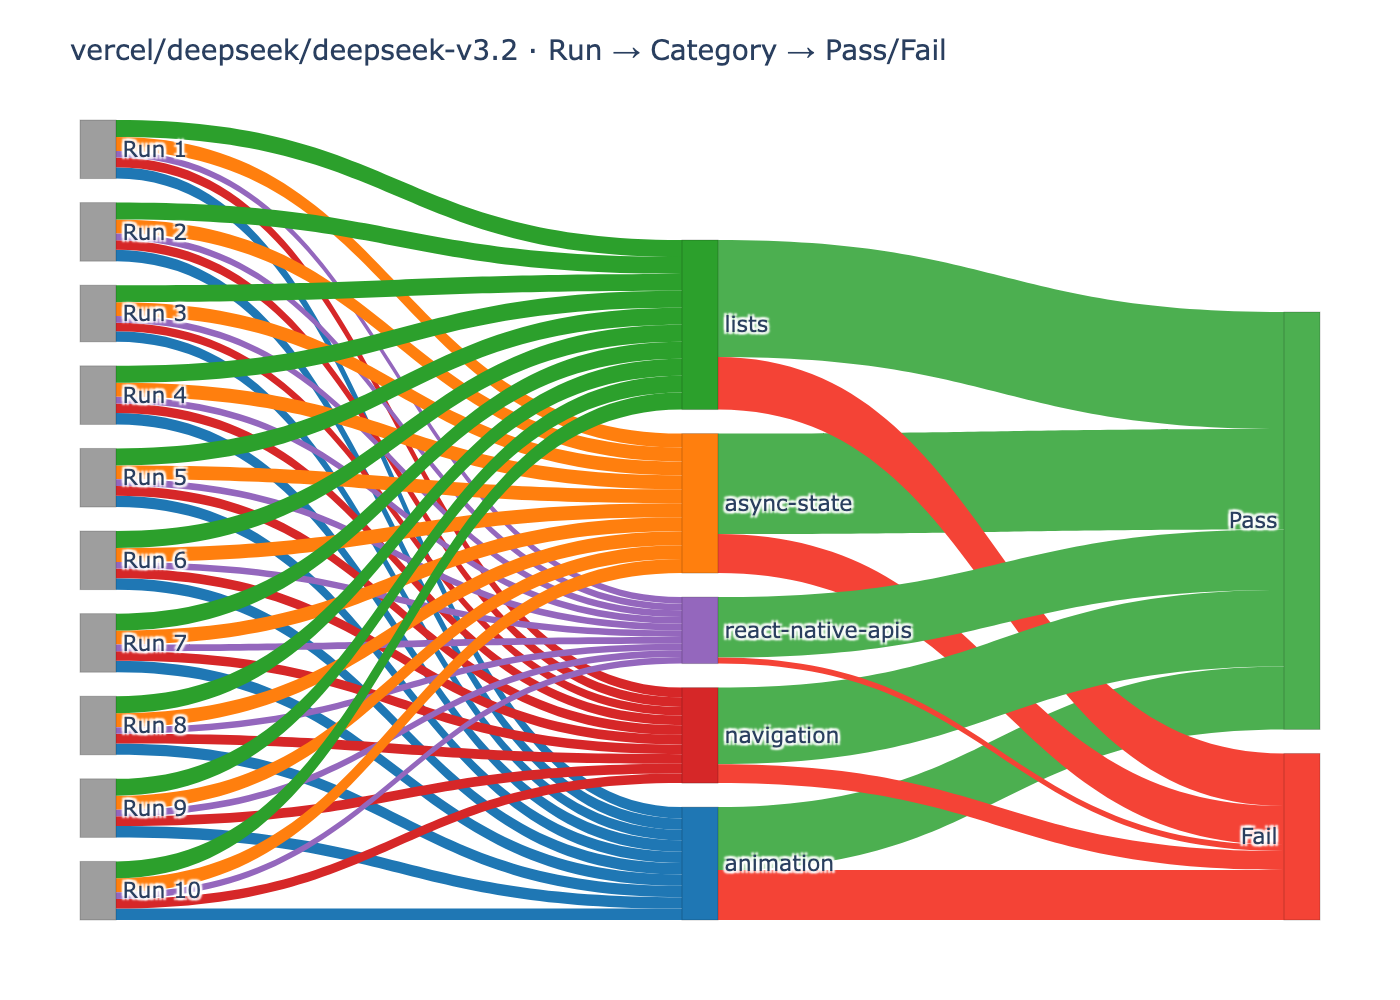
\includegraphics[width=\textwidth]{export/figures/deepseek-v3.2_sankey_per_run.png}
\caption{Sankey per run for deepseek-v3.2 showing the distribution of evals with respect to categories and results}
\end{figure}


\clearpage

\subsection{gemini-3.1-pro-preview}

% Table: summary
\input{export/tables/gemini-3.1-pro-preview_summary}

% Table: category_summary
\input{export/tables/gemini-3.1-pro-preview_category_summary}

% Table: per_eval
\input{export/tables/gemini-3.1-pro-preview_per_eval}

\begin{figure}[htbp]
\centering
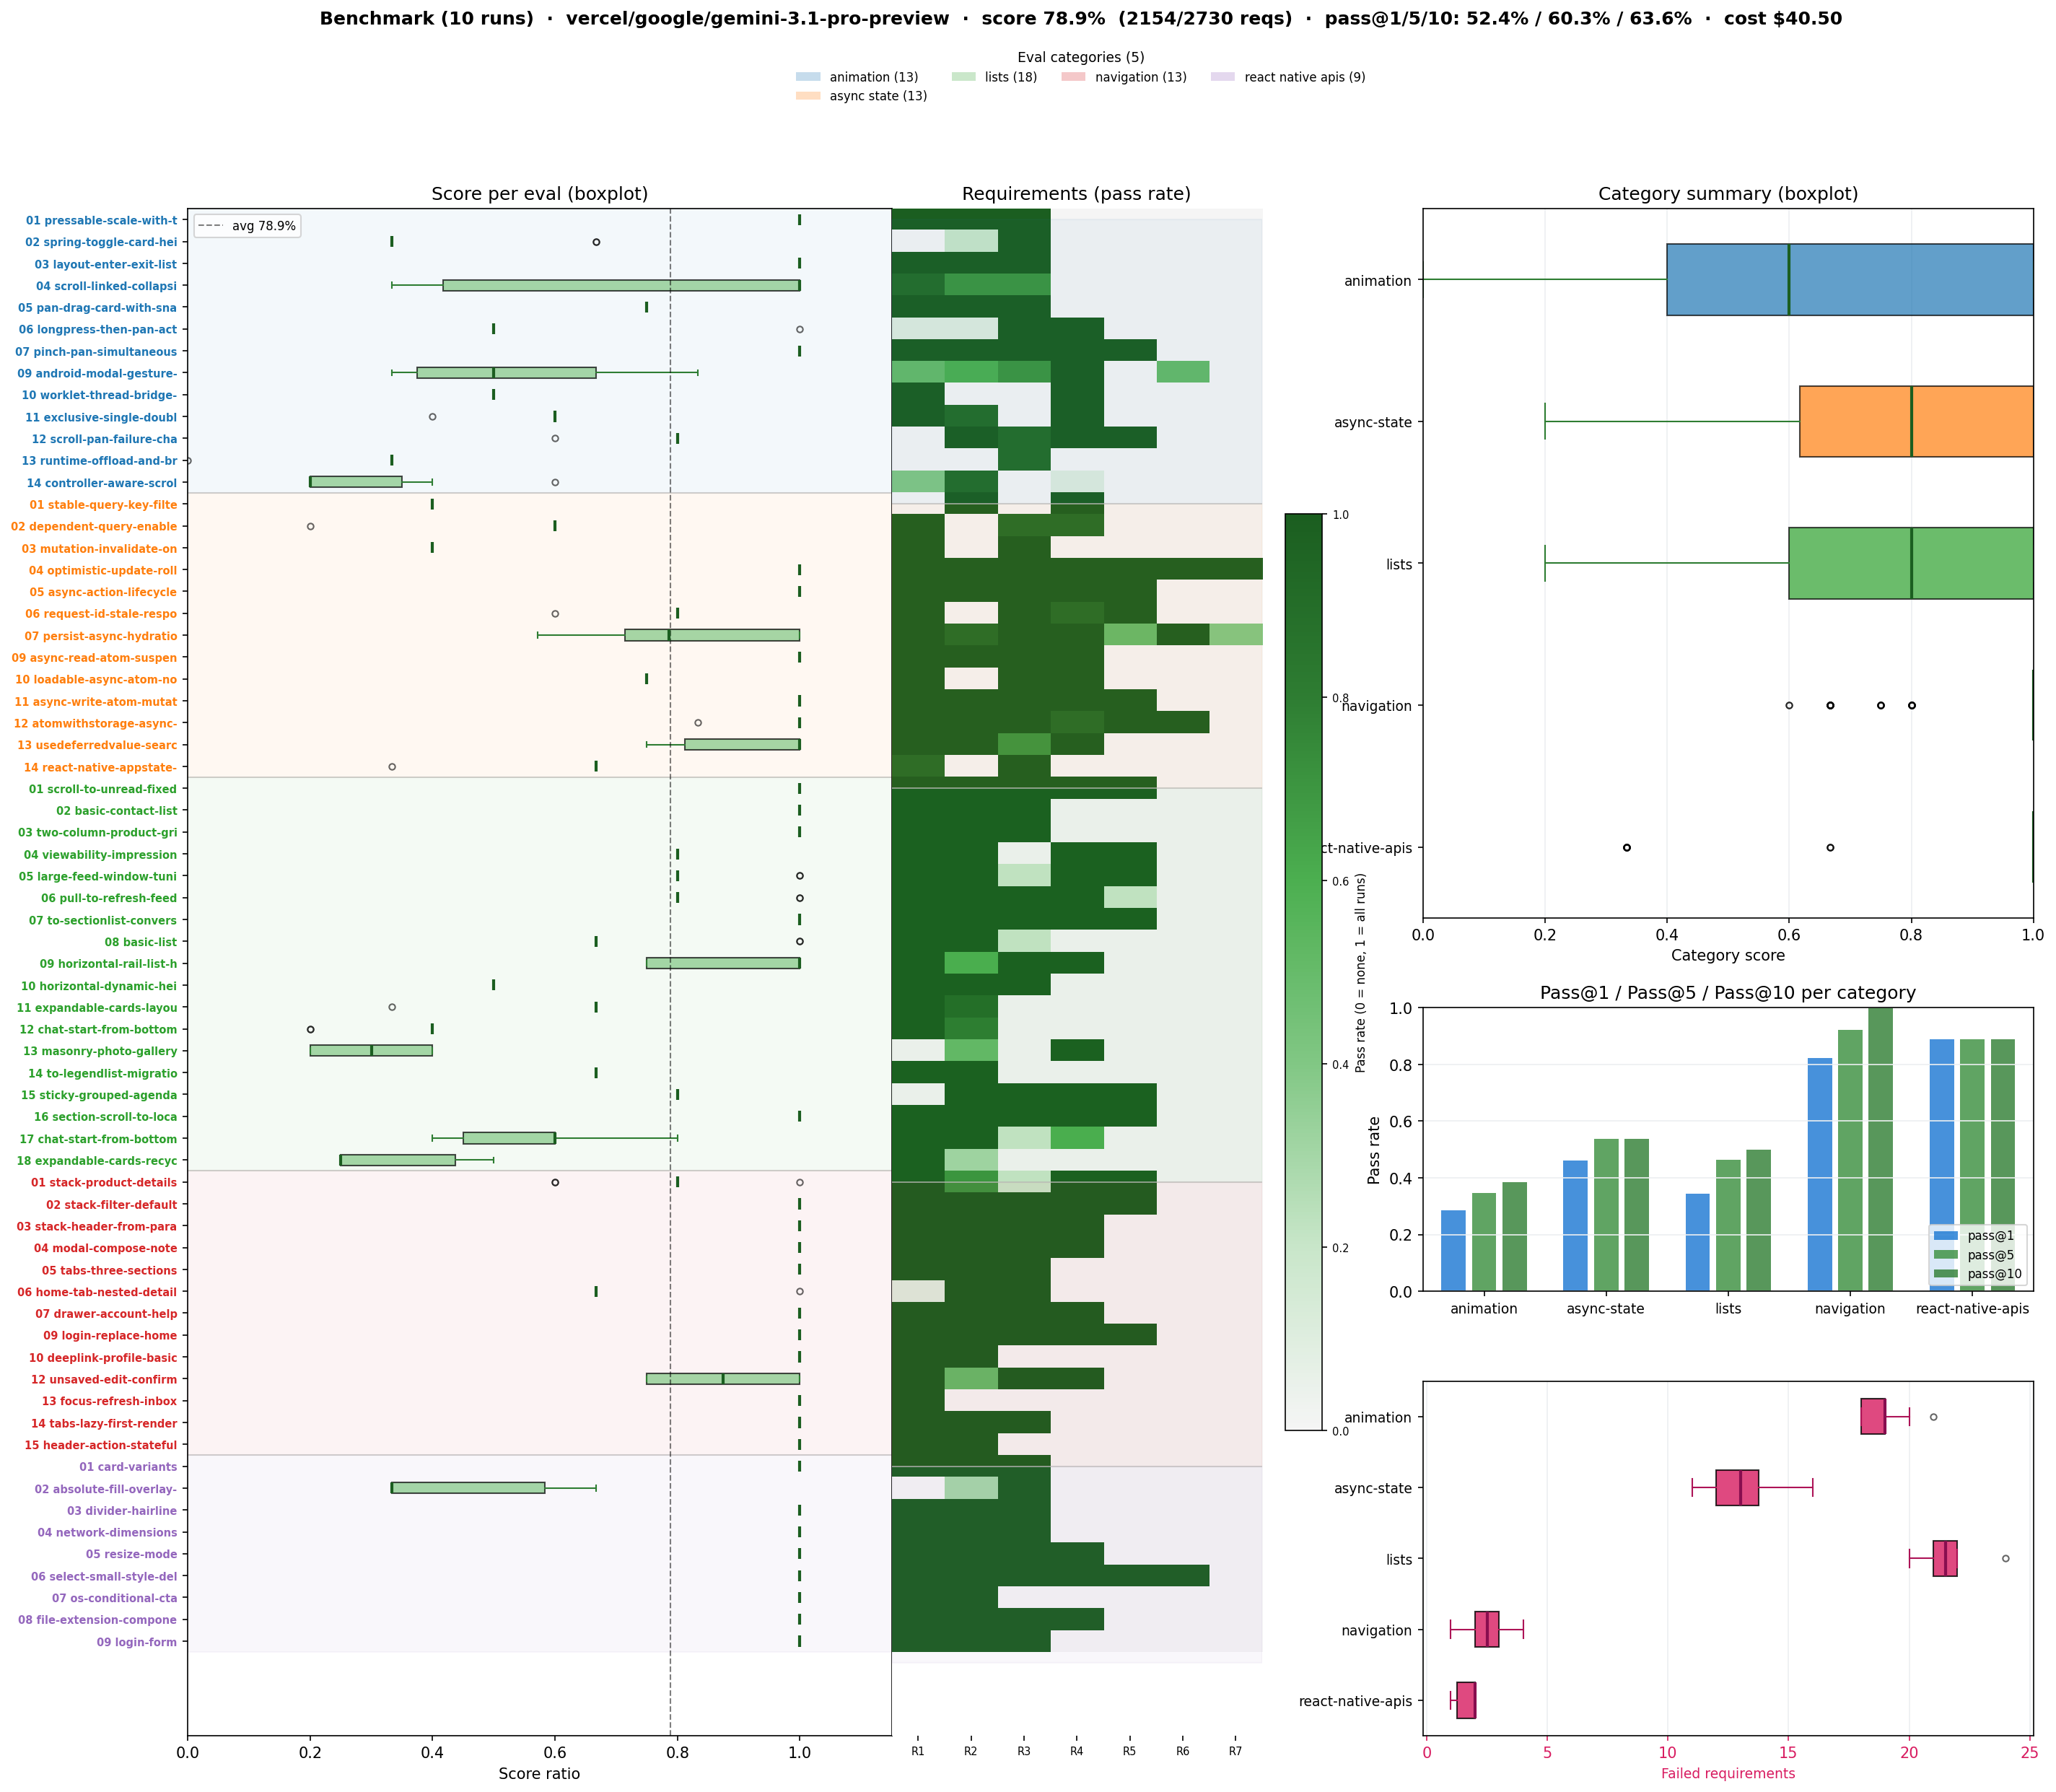
\includegraphics[width=\textwidth]{export/figures/gemini-3.1-pro-preview_benchmark_plot.png}
\caption{Benchmark Plot for gemini-3.1-pro-preview.}
\end{figure}

\begin{figure}[htbp]
\centering
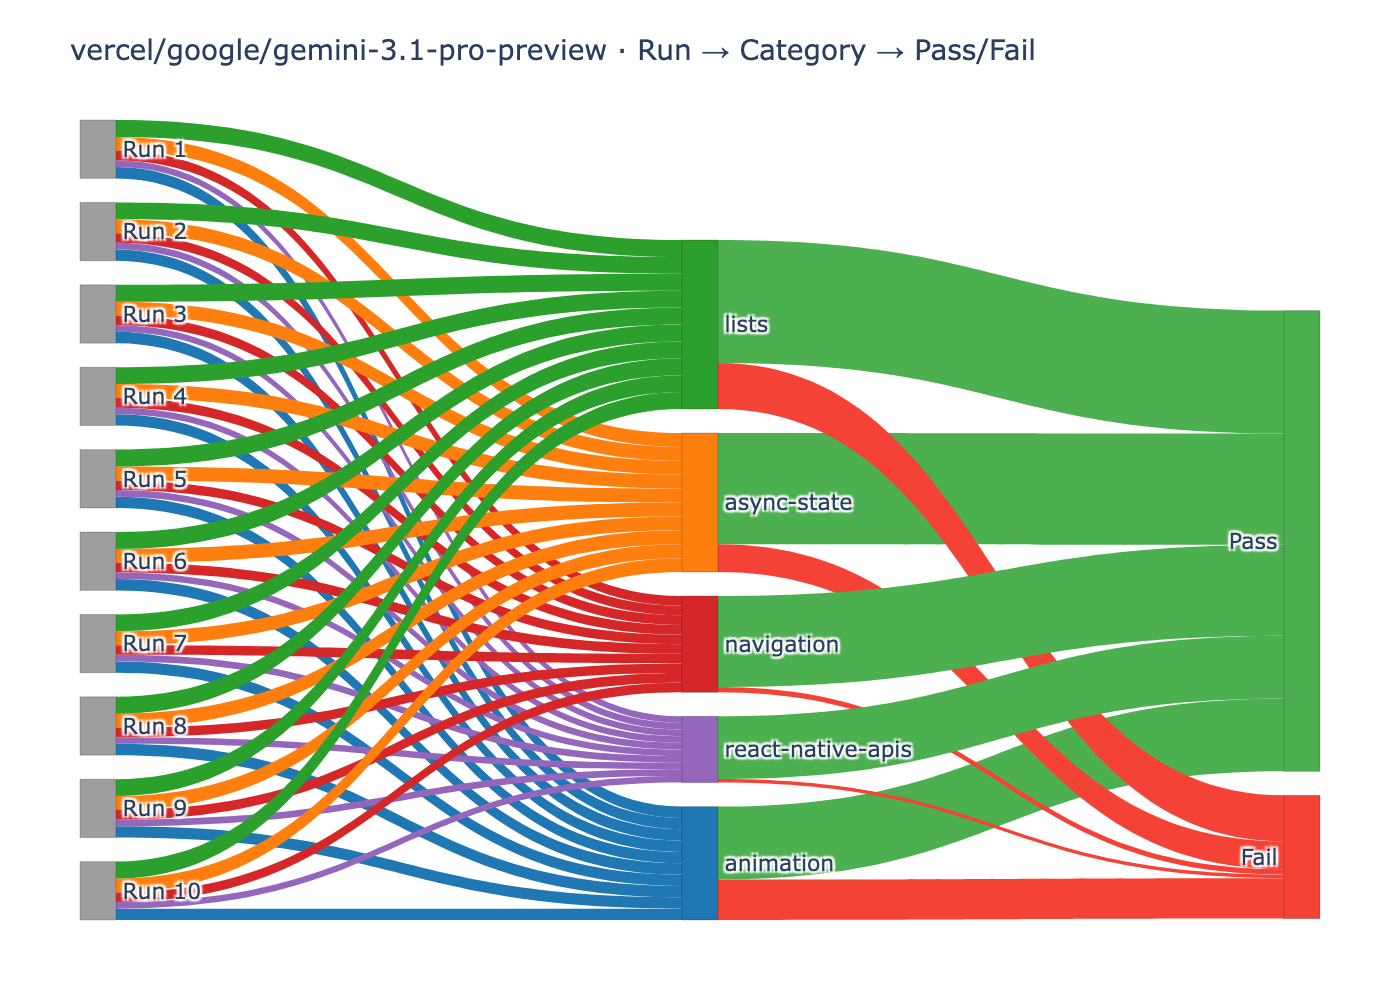
\includegraphics[width=\textwidth]{export/figures/gemini-3.1-pro-preview_sankey_per_run.png}
\caption{Sankey per run for gemini-3.1-pro-preview showing the distribution of evals with respect to categories and results}
\end{figure}


\clearpage

\subsection{glm-5}

% Table: summary
\input{export/tables/glm-5_summary}

% Table: category_summary
\input{export/tables/glm-5_category_summary}

% Table: per_eval
\input{export/tables/glm-5_per_eval}

\begin{figure}[htbp]
\centering
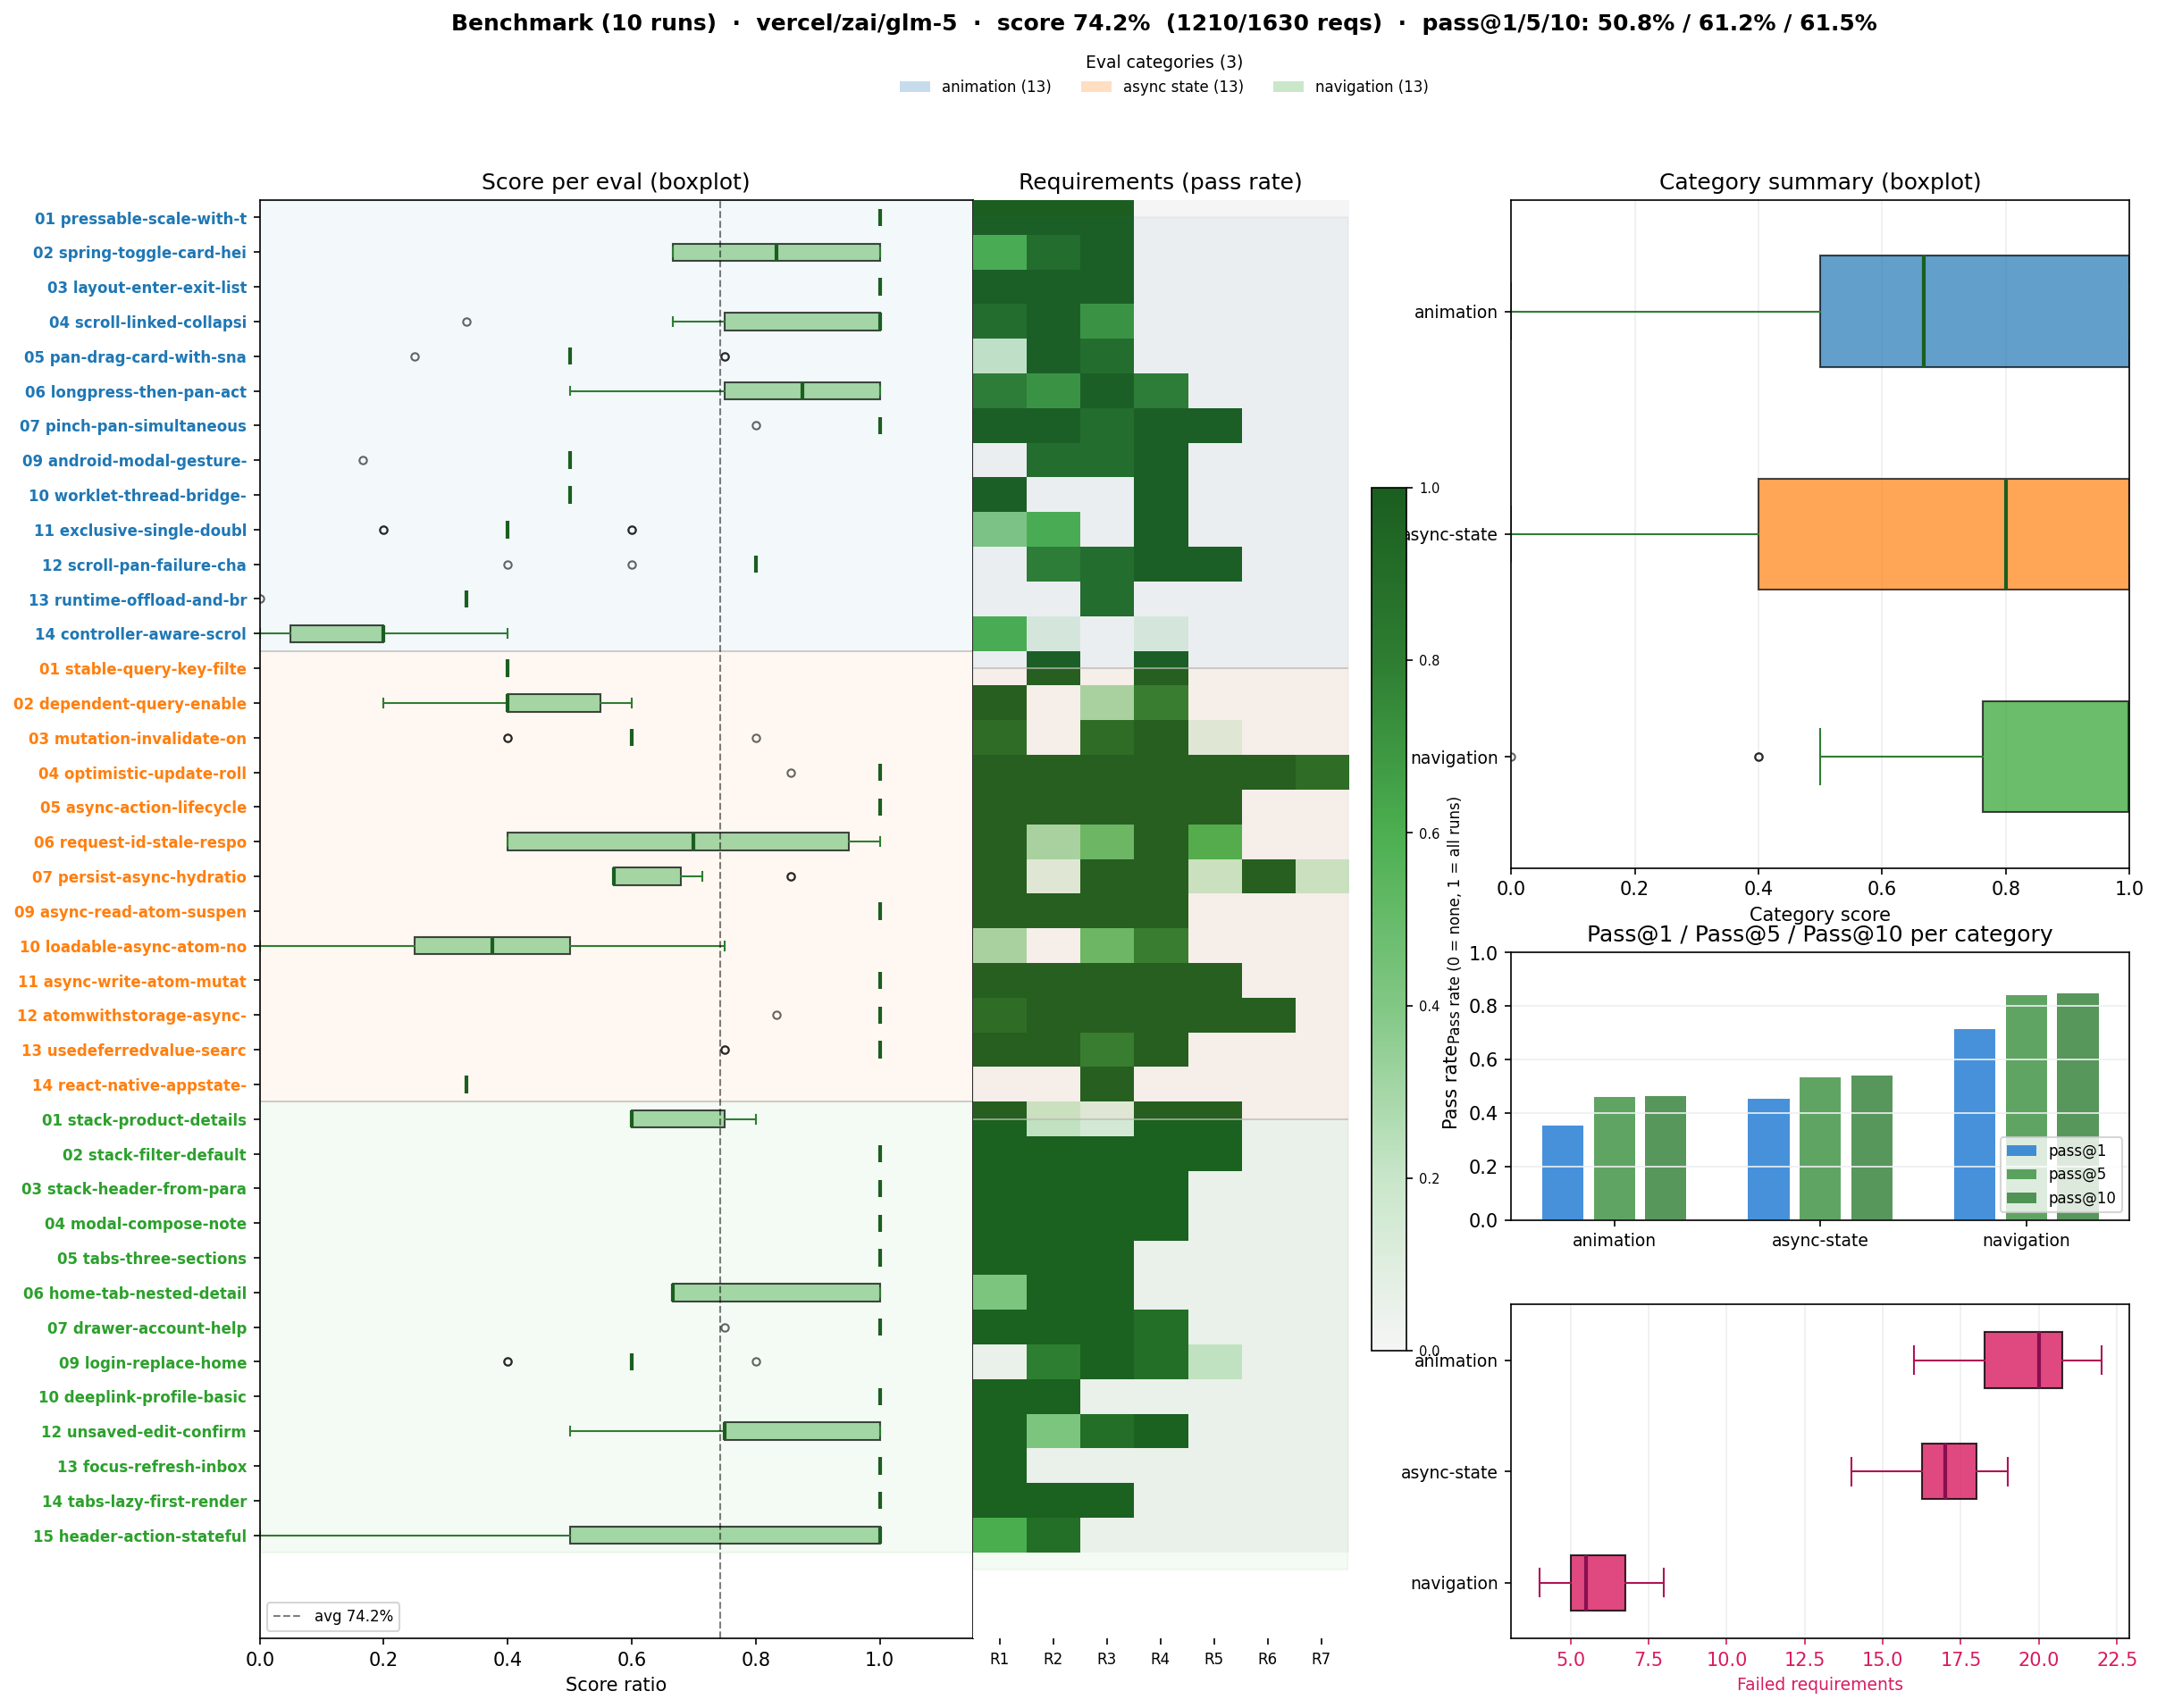
\includegraphics[width=\textwidth]{export/figures/glm-5_benchmark_plot.png}
\caption{Benchmark Plot for glm-5.}
\end{figure}

\begin{figure}[htbp]
\centering
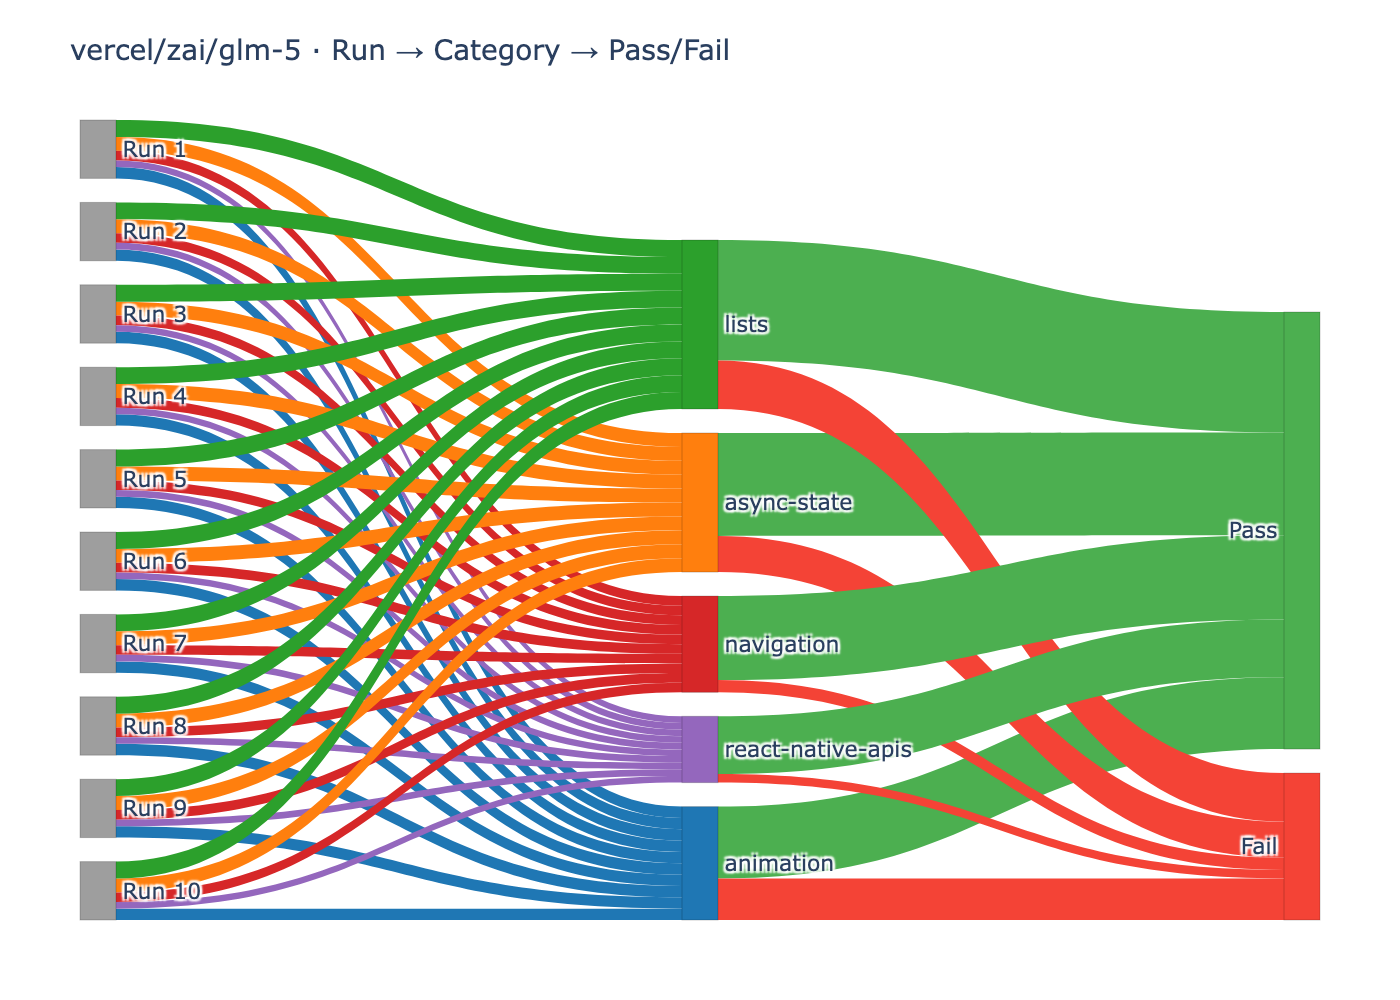
\includegraphics[width=\textwidth]{export/figures/glm-5_sankey_per_run.png}
\caption{Sankey per run for glm-5 showing the distribution of evals with respect to categories and results}
\end{figure}


\clearpage

\subsection{gpt-5.3-codex}

% Table: summary
\input{export/tables/gpt-5.3-codex_summary}

% Table: category_summary
\input{export/tables/gpt-5.3-codex_category_summary}

% Table: per_eval
\input{export/tables/gpt-5.3-codex_per_eval}

\begin{figure}[htbp]
\centering
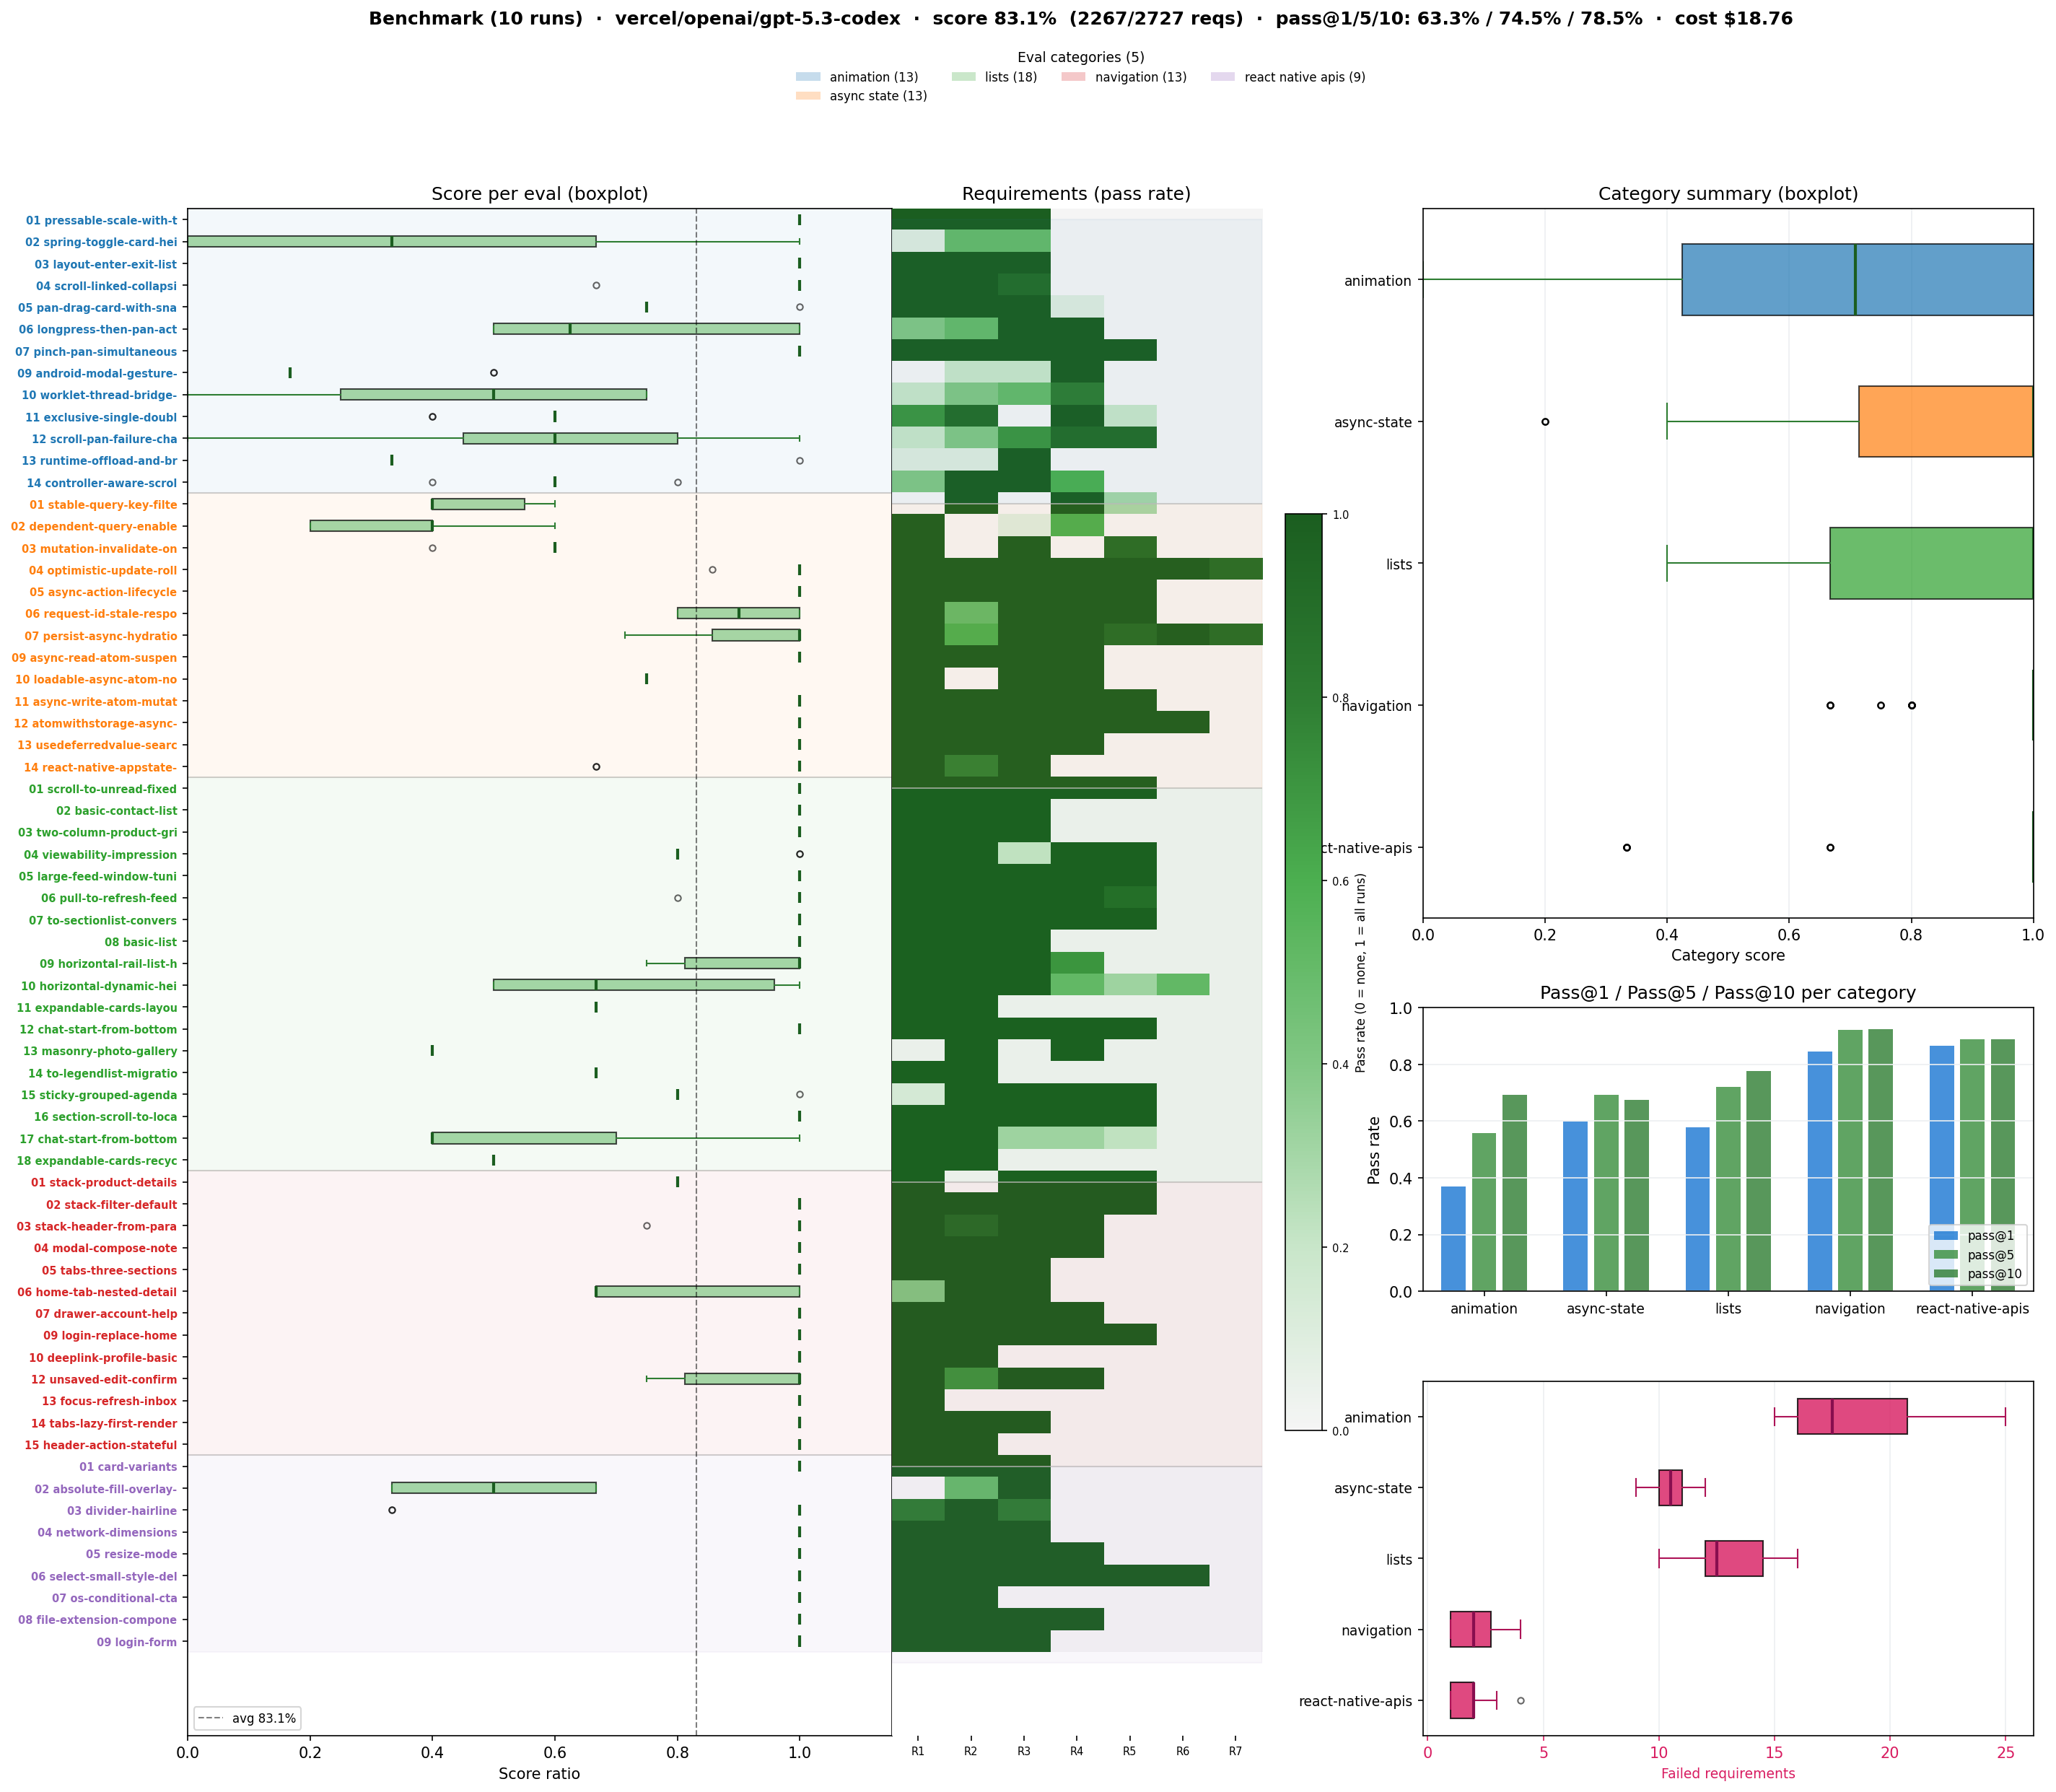
\includegraphics[width=\textwidth]{export/figures/gpt-5.3-codex_benchmark_plot.png}
\caption{Benchmark Plot for gpt-5.3-codex.}
\end{figure}

\begin{figure}[htbp]
\centering
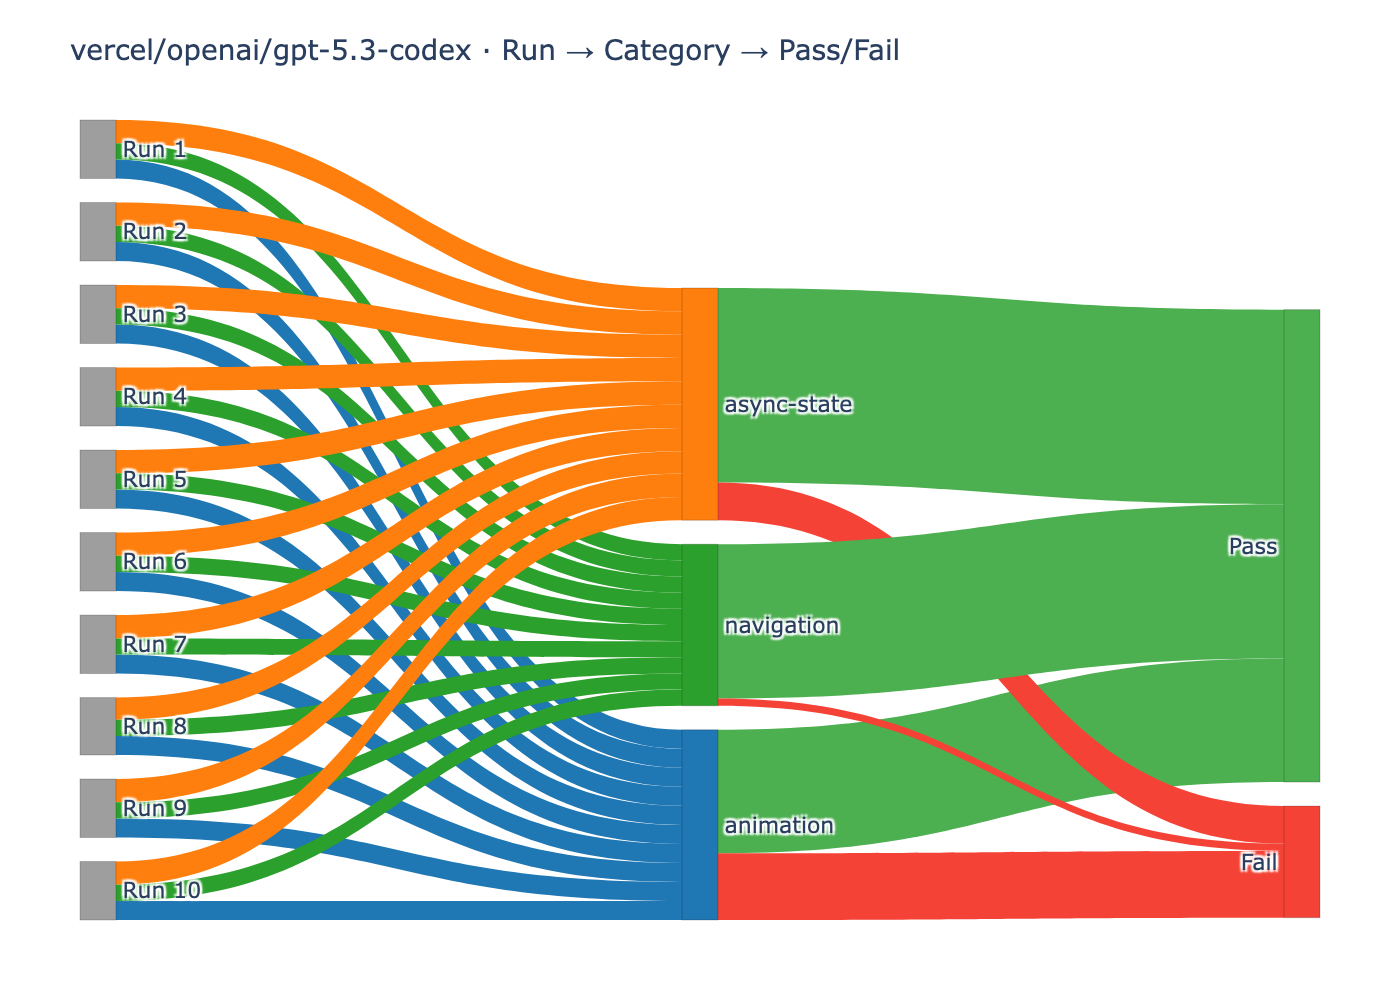
\includegraphics[width=\textwidth]{export/figures/gpt-5.3-codex_sankey_per_run.png}
\caption{Sankey per run for gpt-5.3-codex showing the distribution of evals with respect to categories and results}
\end{figure}


\clearpage

\subsection{gpt-5.4}

% Table: summary
\input{export/tables/gpt-5.4_summary}

% Table: category_summary
\input{export/tables/gpt-5.4_category_summary}

% Table: per_eval
\input{export/tables/gpt-5.4_per_eval}

\begin{figure}[htbp]
\centering
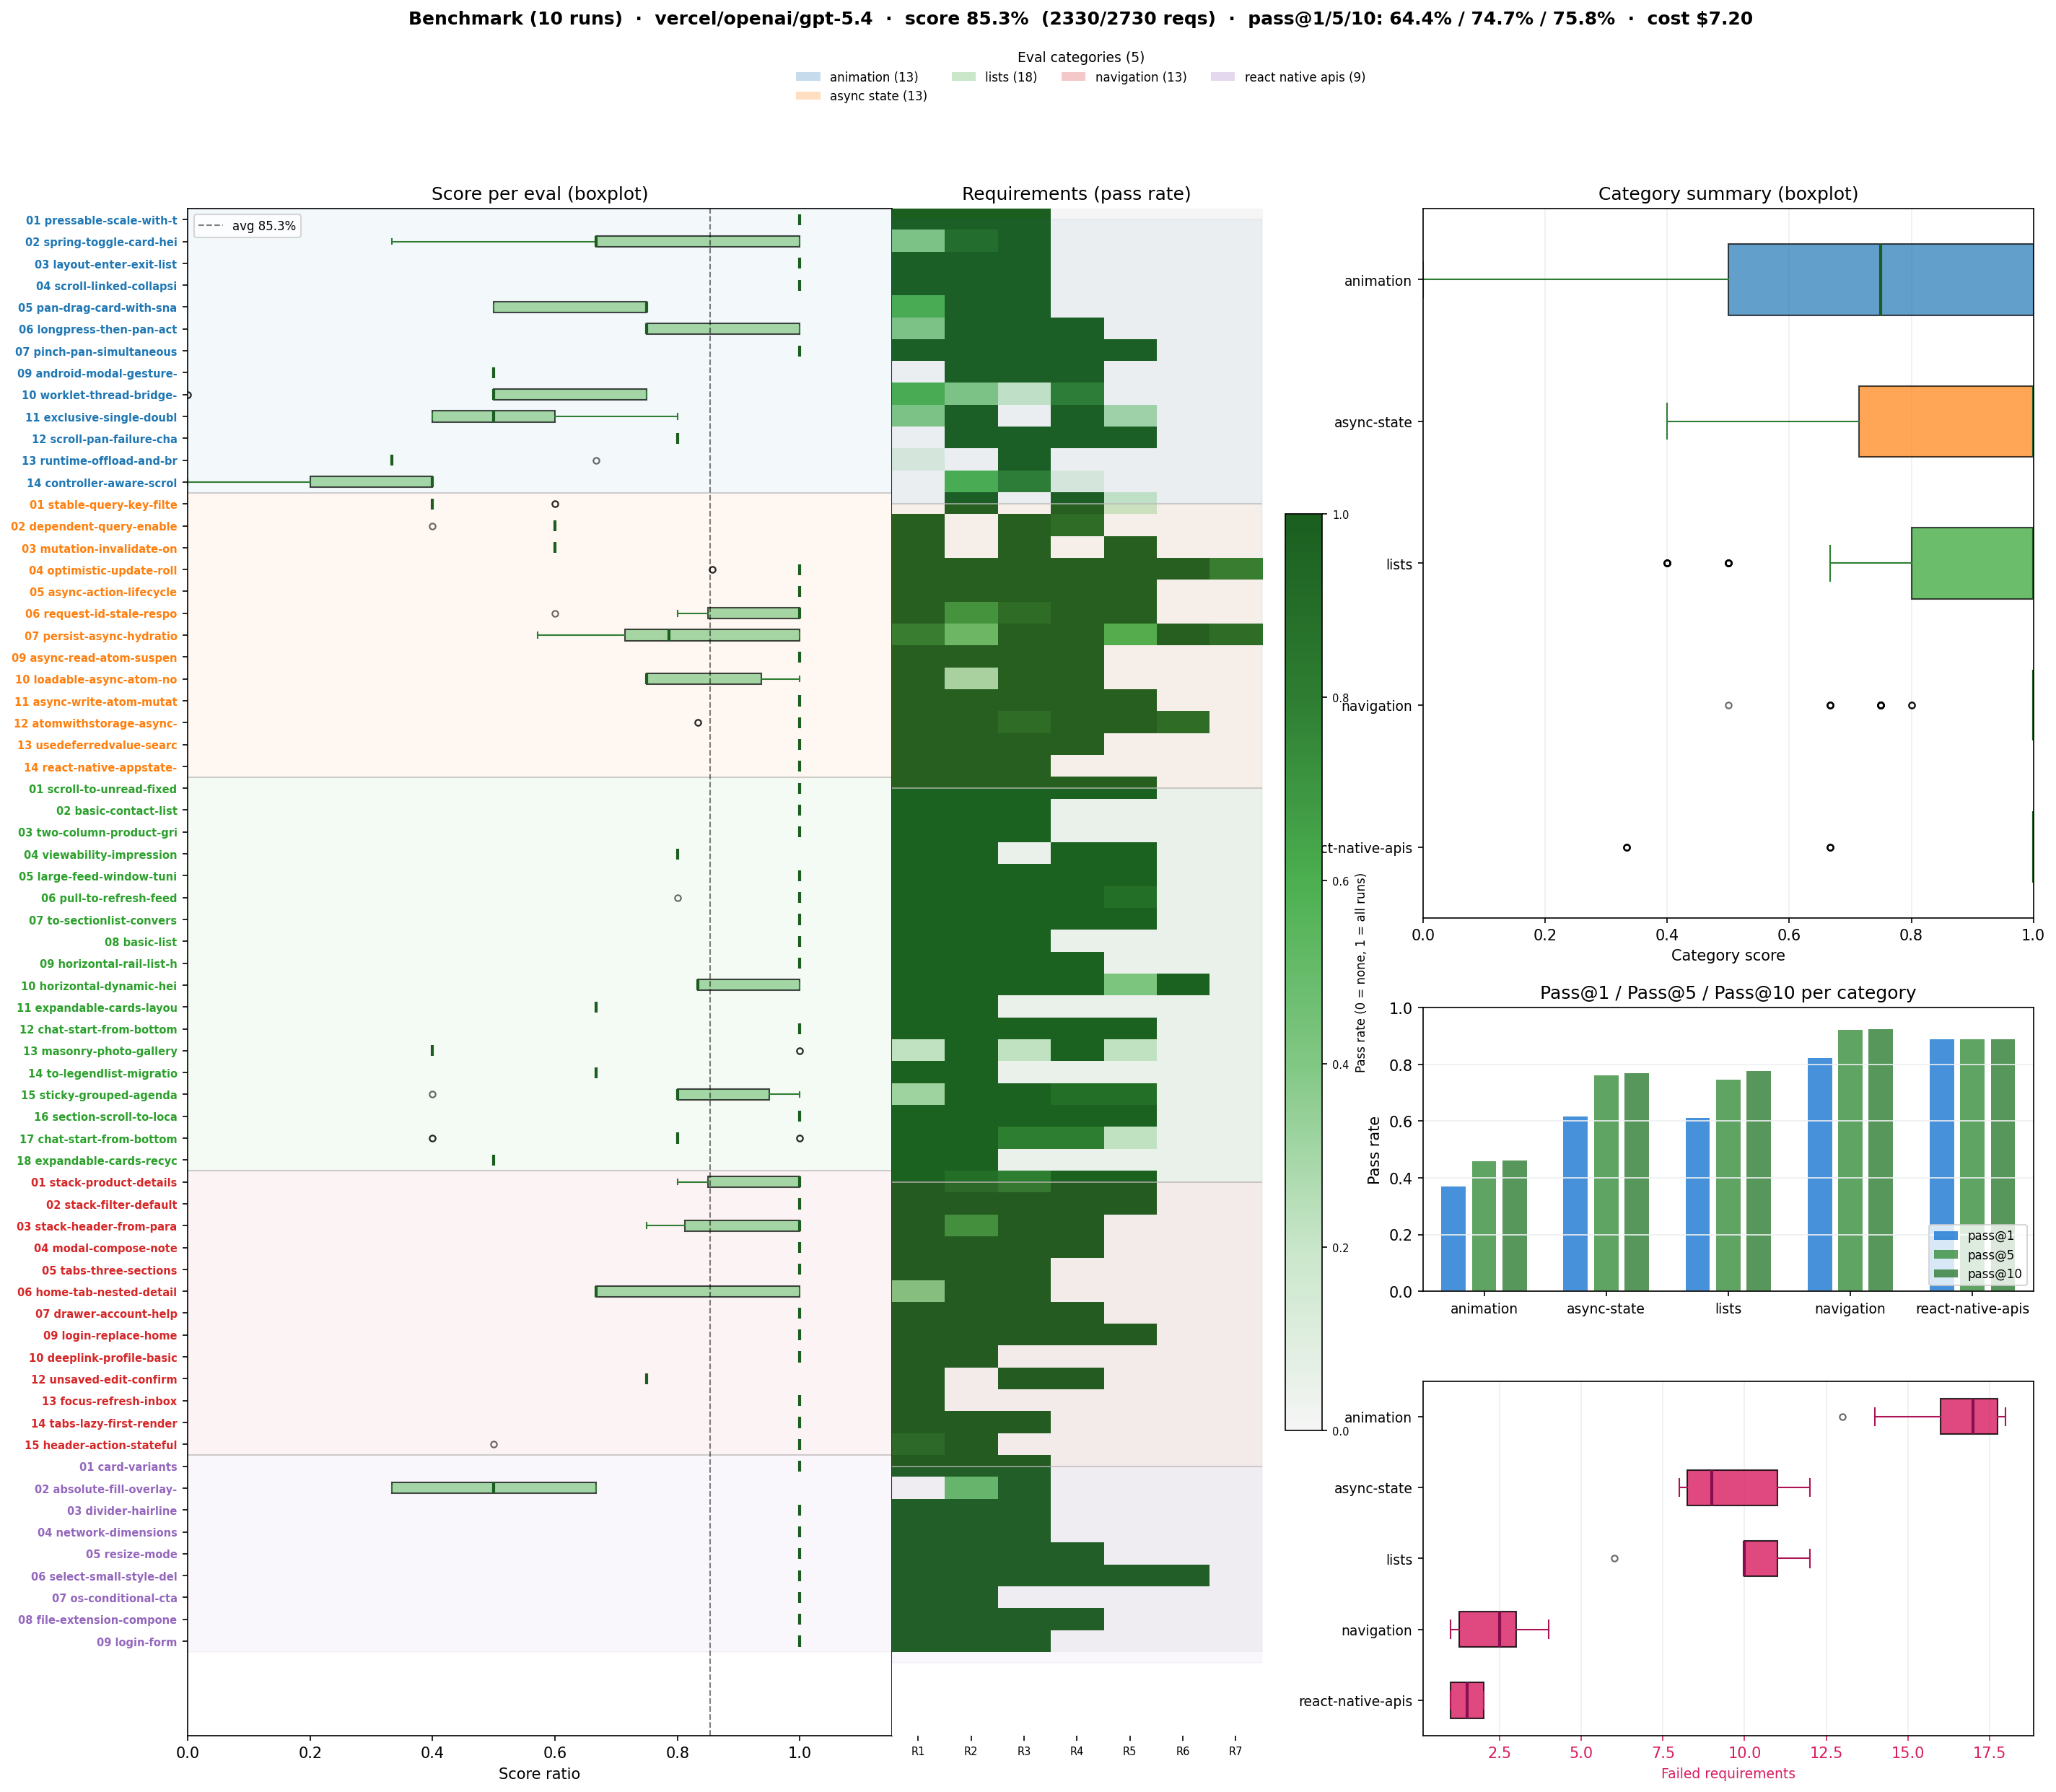
\includegraphics[width=\textwidth]{export/figures/gpt-5.4_benchmark_plot.png}
\caption{Benchmark Plot for gpt-5.4.}
\end{figure}

\begin{figure}[htbp]
\centering
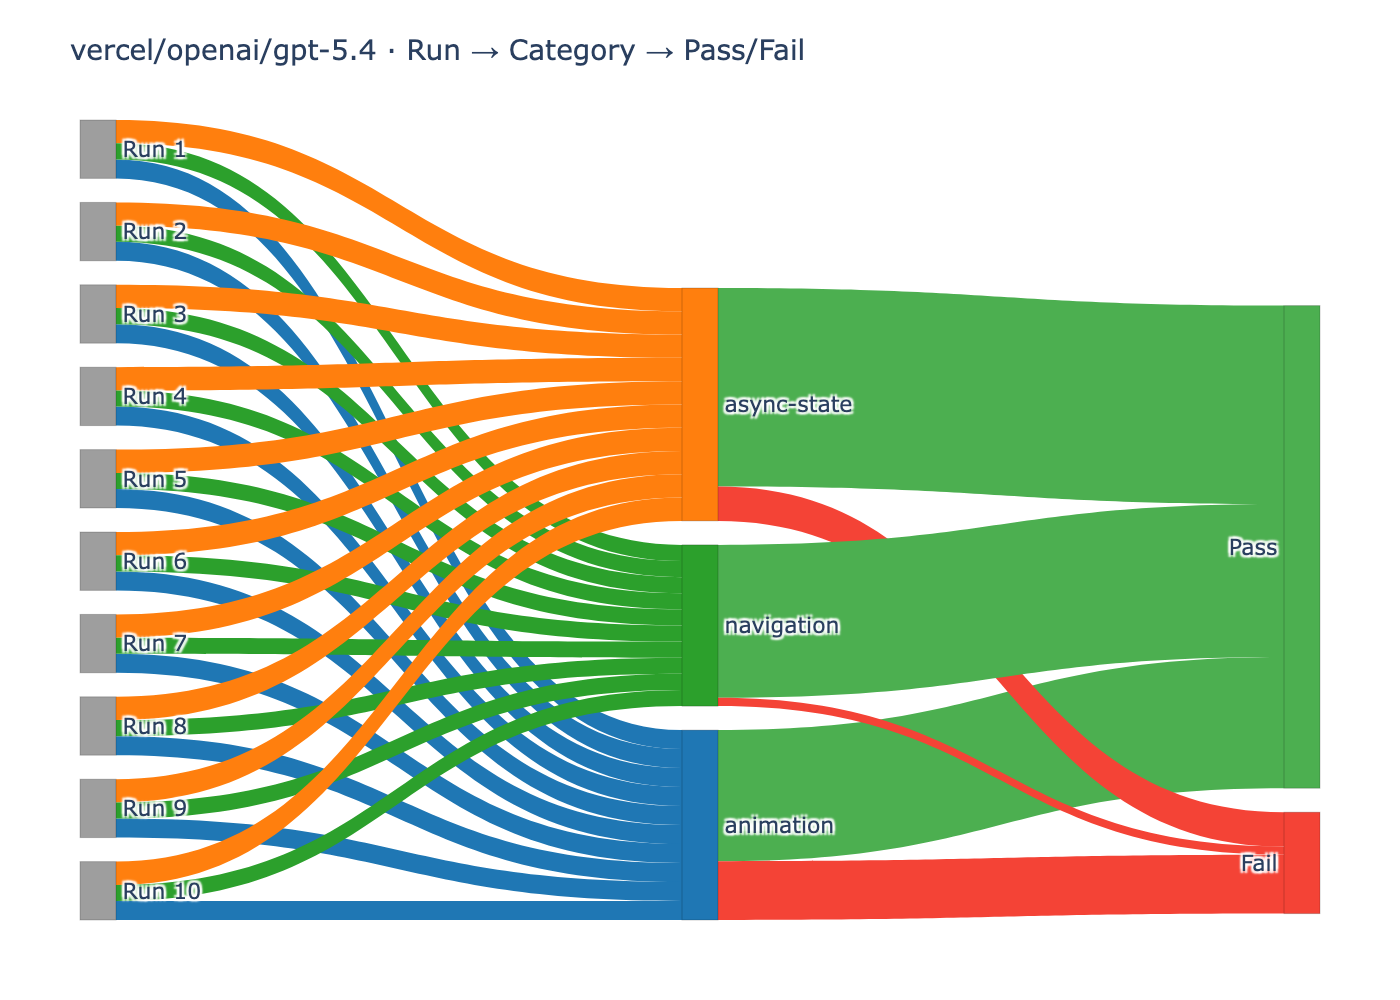
\includegraphics[width=\textwidth]{export/figures/gpt-5.4_sankey_per_run.png}
\caption{Sankey per run for gpt-5.4 showing the distribution of evals with respect to categories and results}
\end{figure}


\clearpage

\subsection{gpt-oss-120b}

% Table: summary
\input{export/tables/gpt-oss-120b_summary}

% Table: category_summary
\input{export/tables/gpt-oss-120b_category_summary}

% Table: per_eval
\input{export/tables/gpt-oss-120b_per_eval}

\begin{figure}[htbp]
\centering
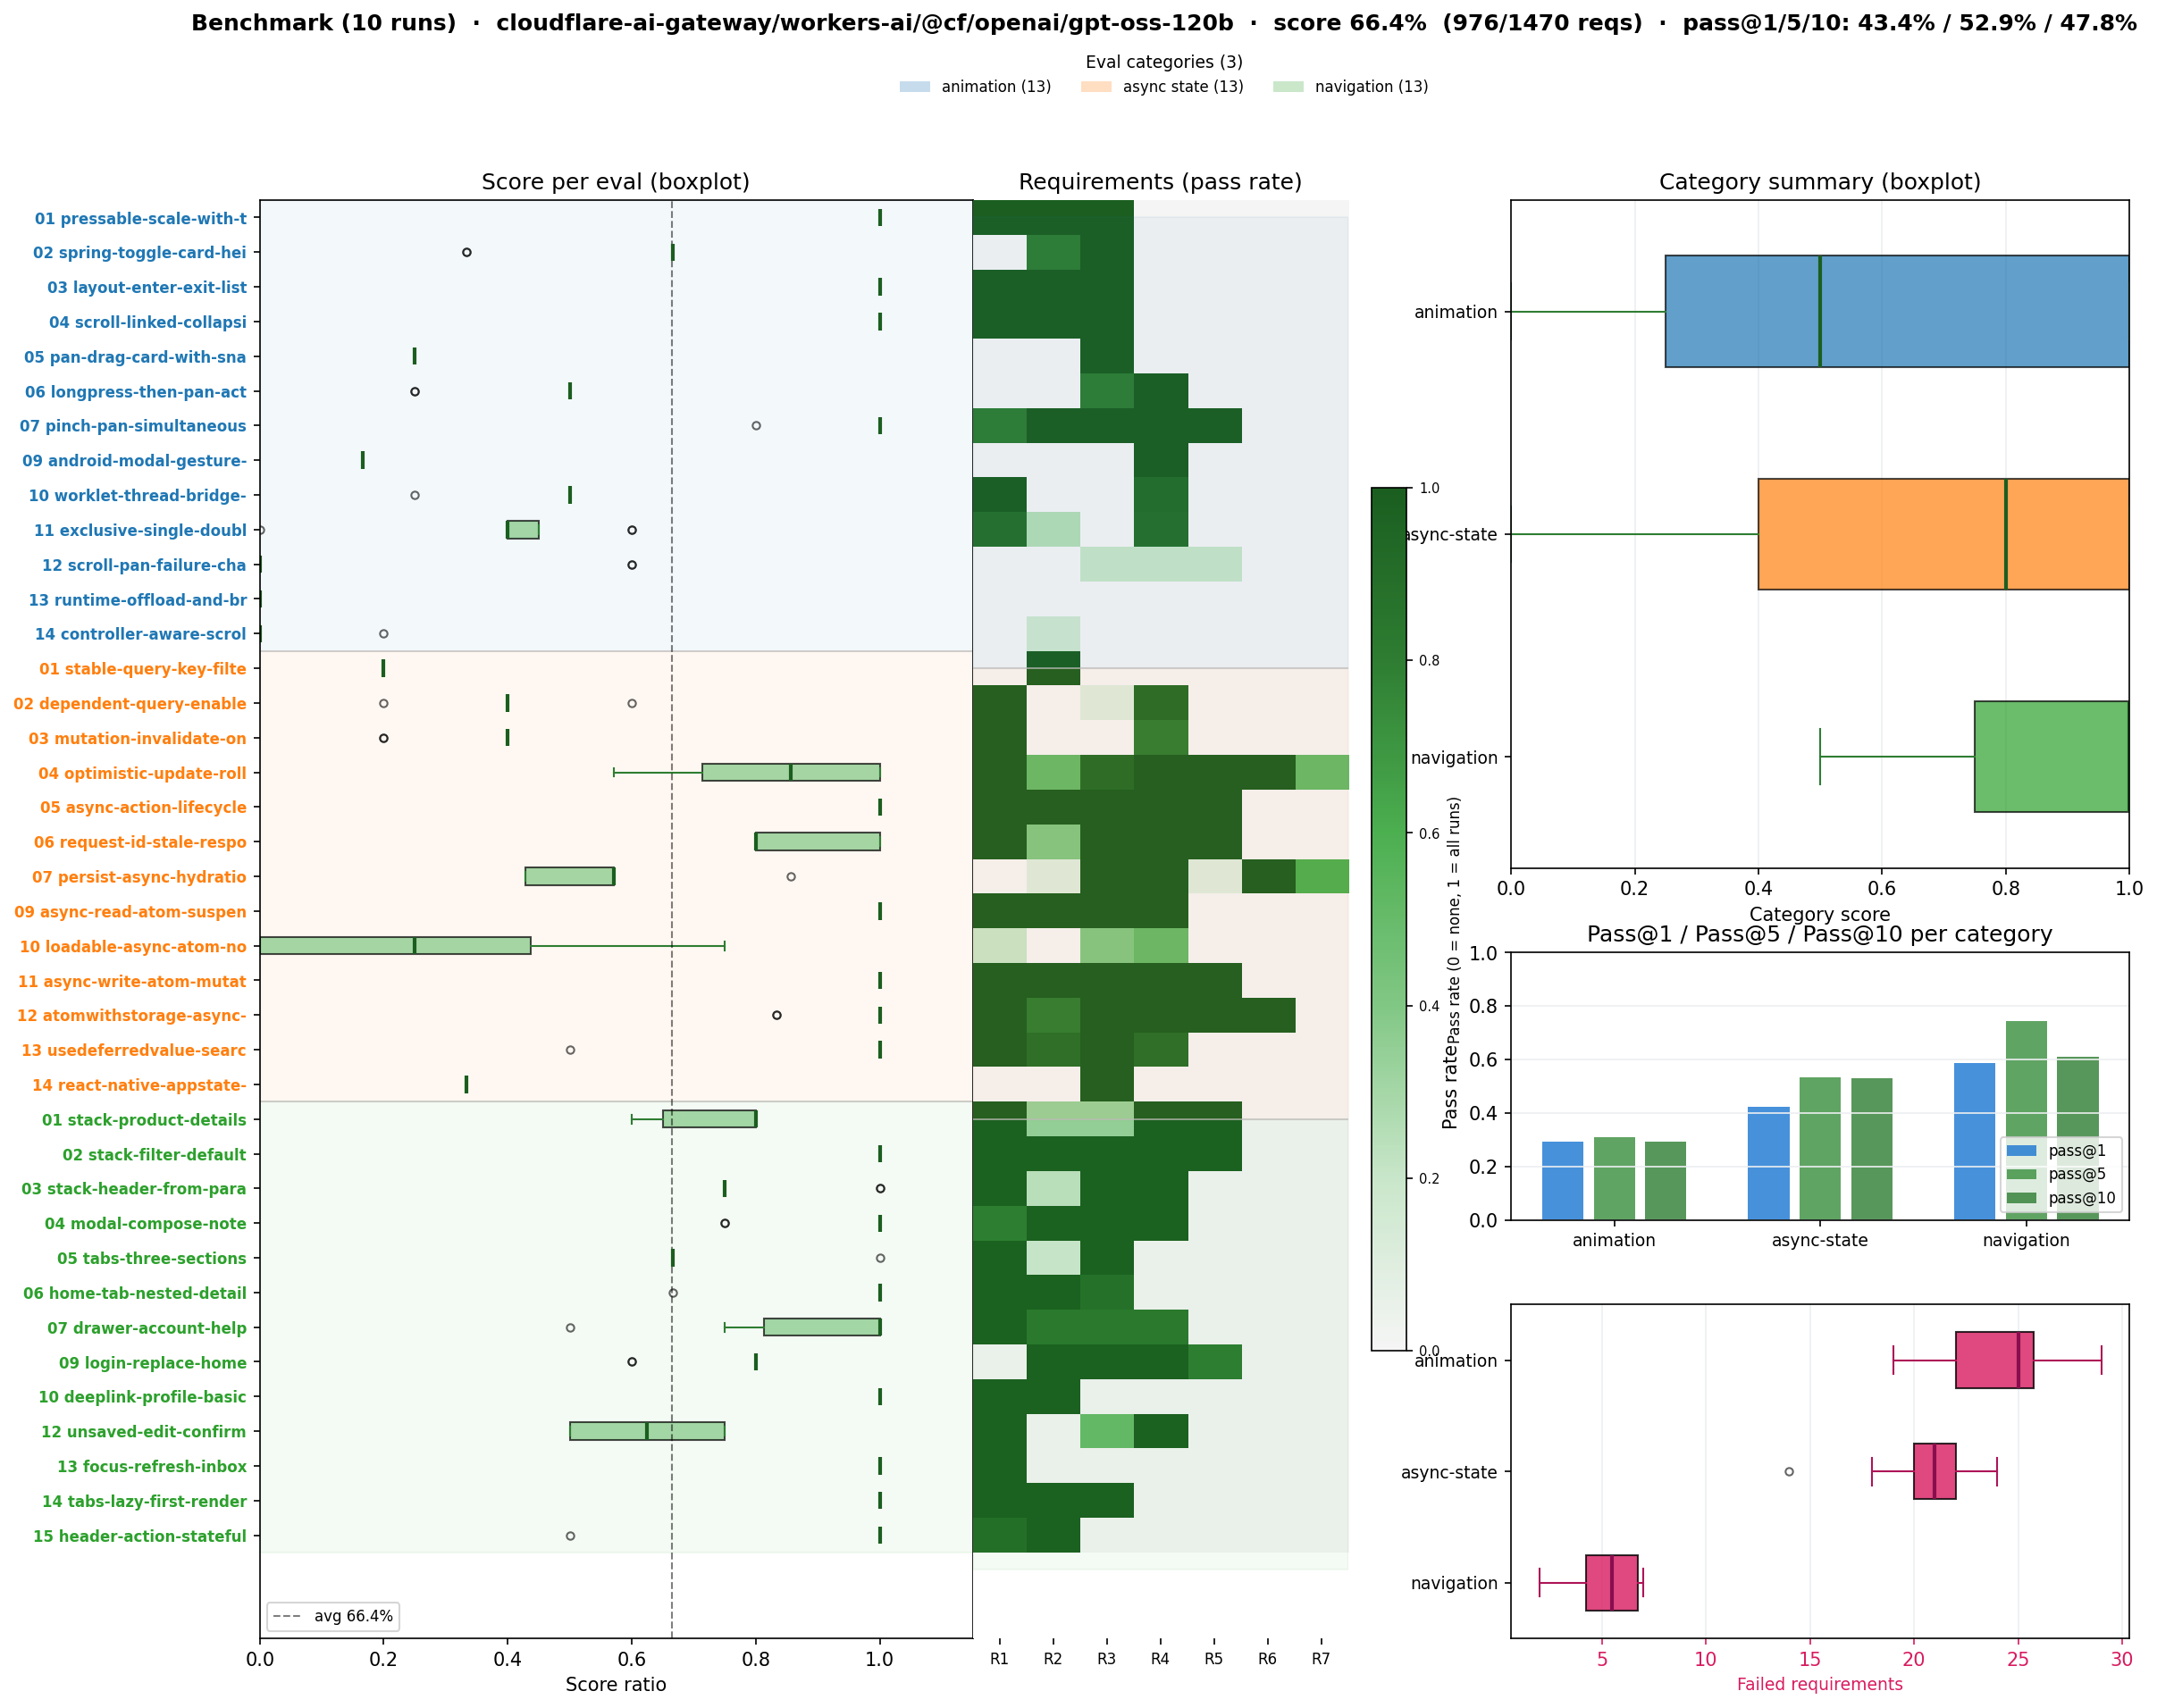
\includegraphics[width=\textwidth]{export/figures/gpt-oss-120b_benchmark_plot.png}
\caption{Benchmark Plot for gpt-oss-120b.}
\end{figure}

\begin{figure}[htbp]
\centering
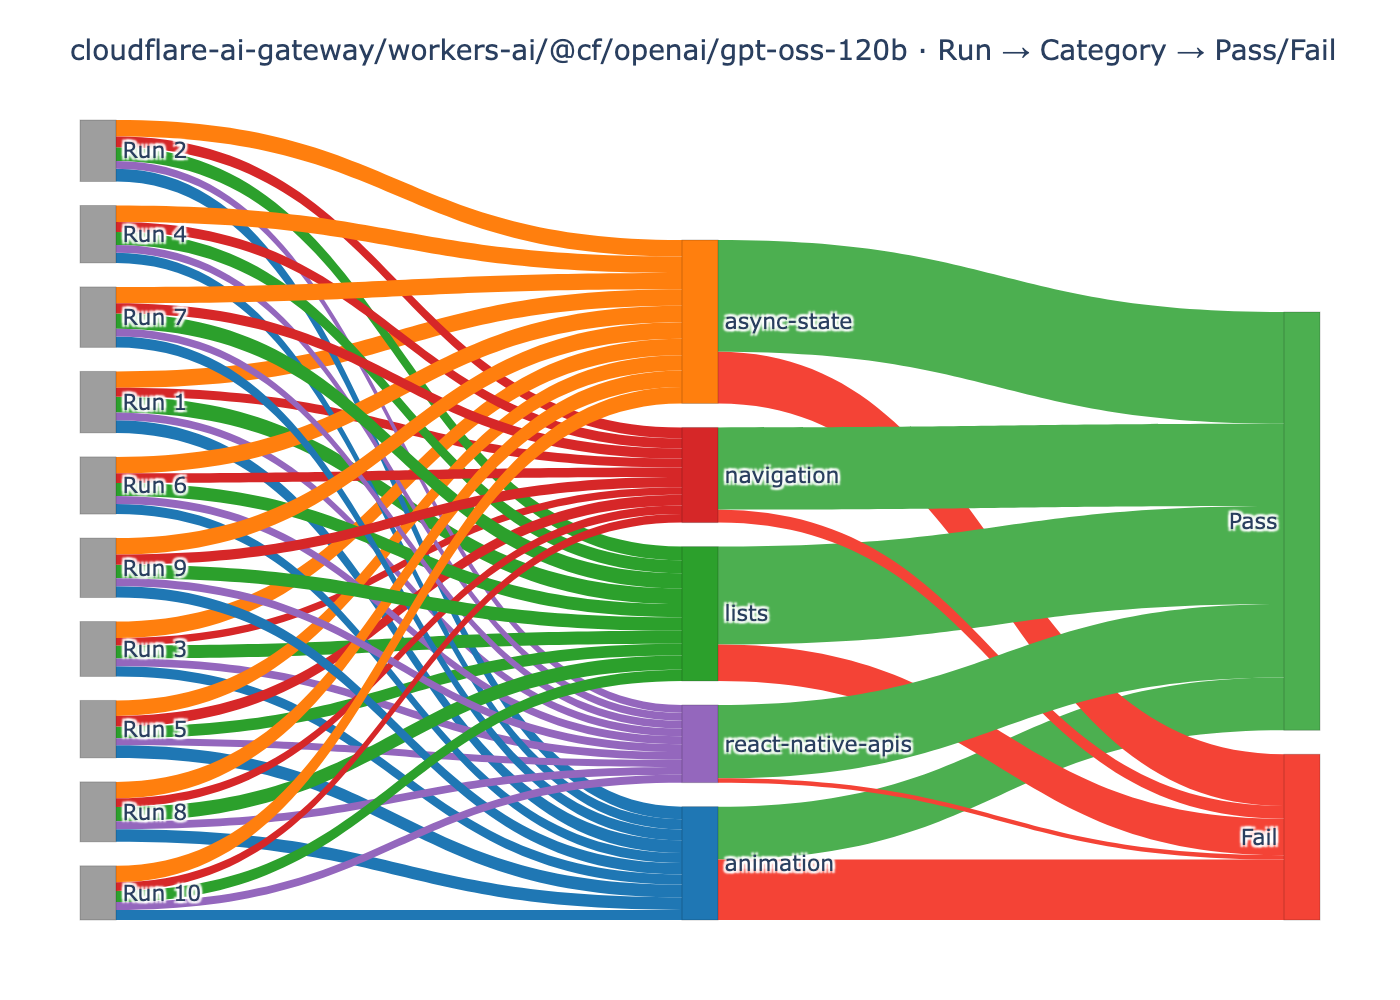
\includegraphics[width=\textwidth]{export/figures/gpt-oss-120b_sankey_per_run.png}
\caption{Sankey per run for gpt-oss-120b showing the distribution of evals with respect to categories and results}
\end{figure}


\clearpage

\subsection{gpt-oss-20b}

% Table: summary
\input{export/tables/gpt-oss-20b_summary}

% Table: category_summary
\input{export/tables/gpt-oss-20b_category_summary}

% Table: per_eval
\input{export/tables/gpt-oss-20b_per_eval}

\begin{figure}[htbp]
\centering
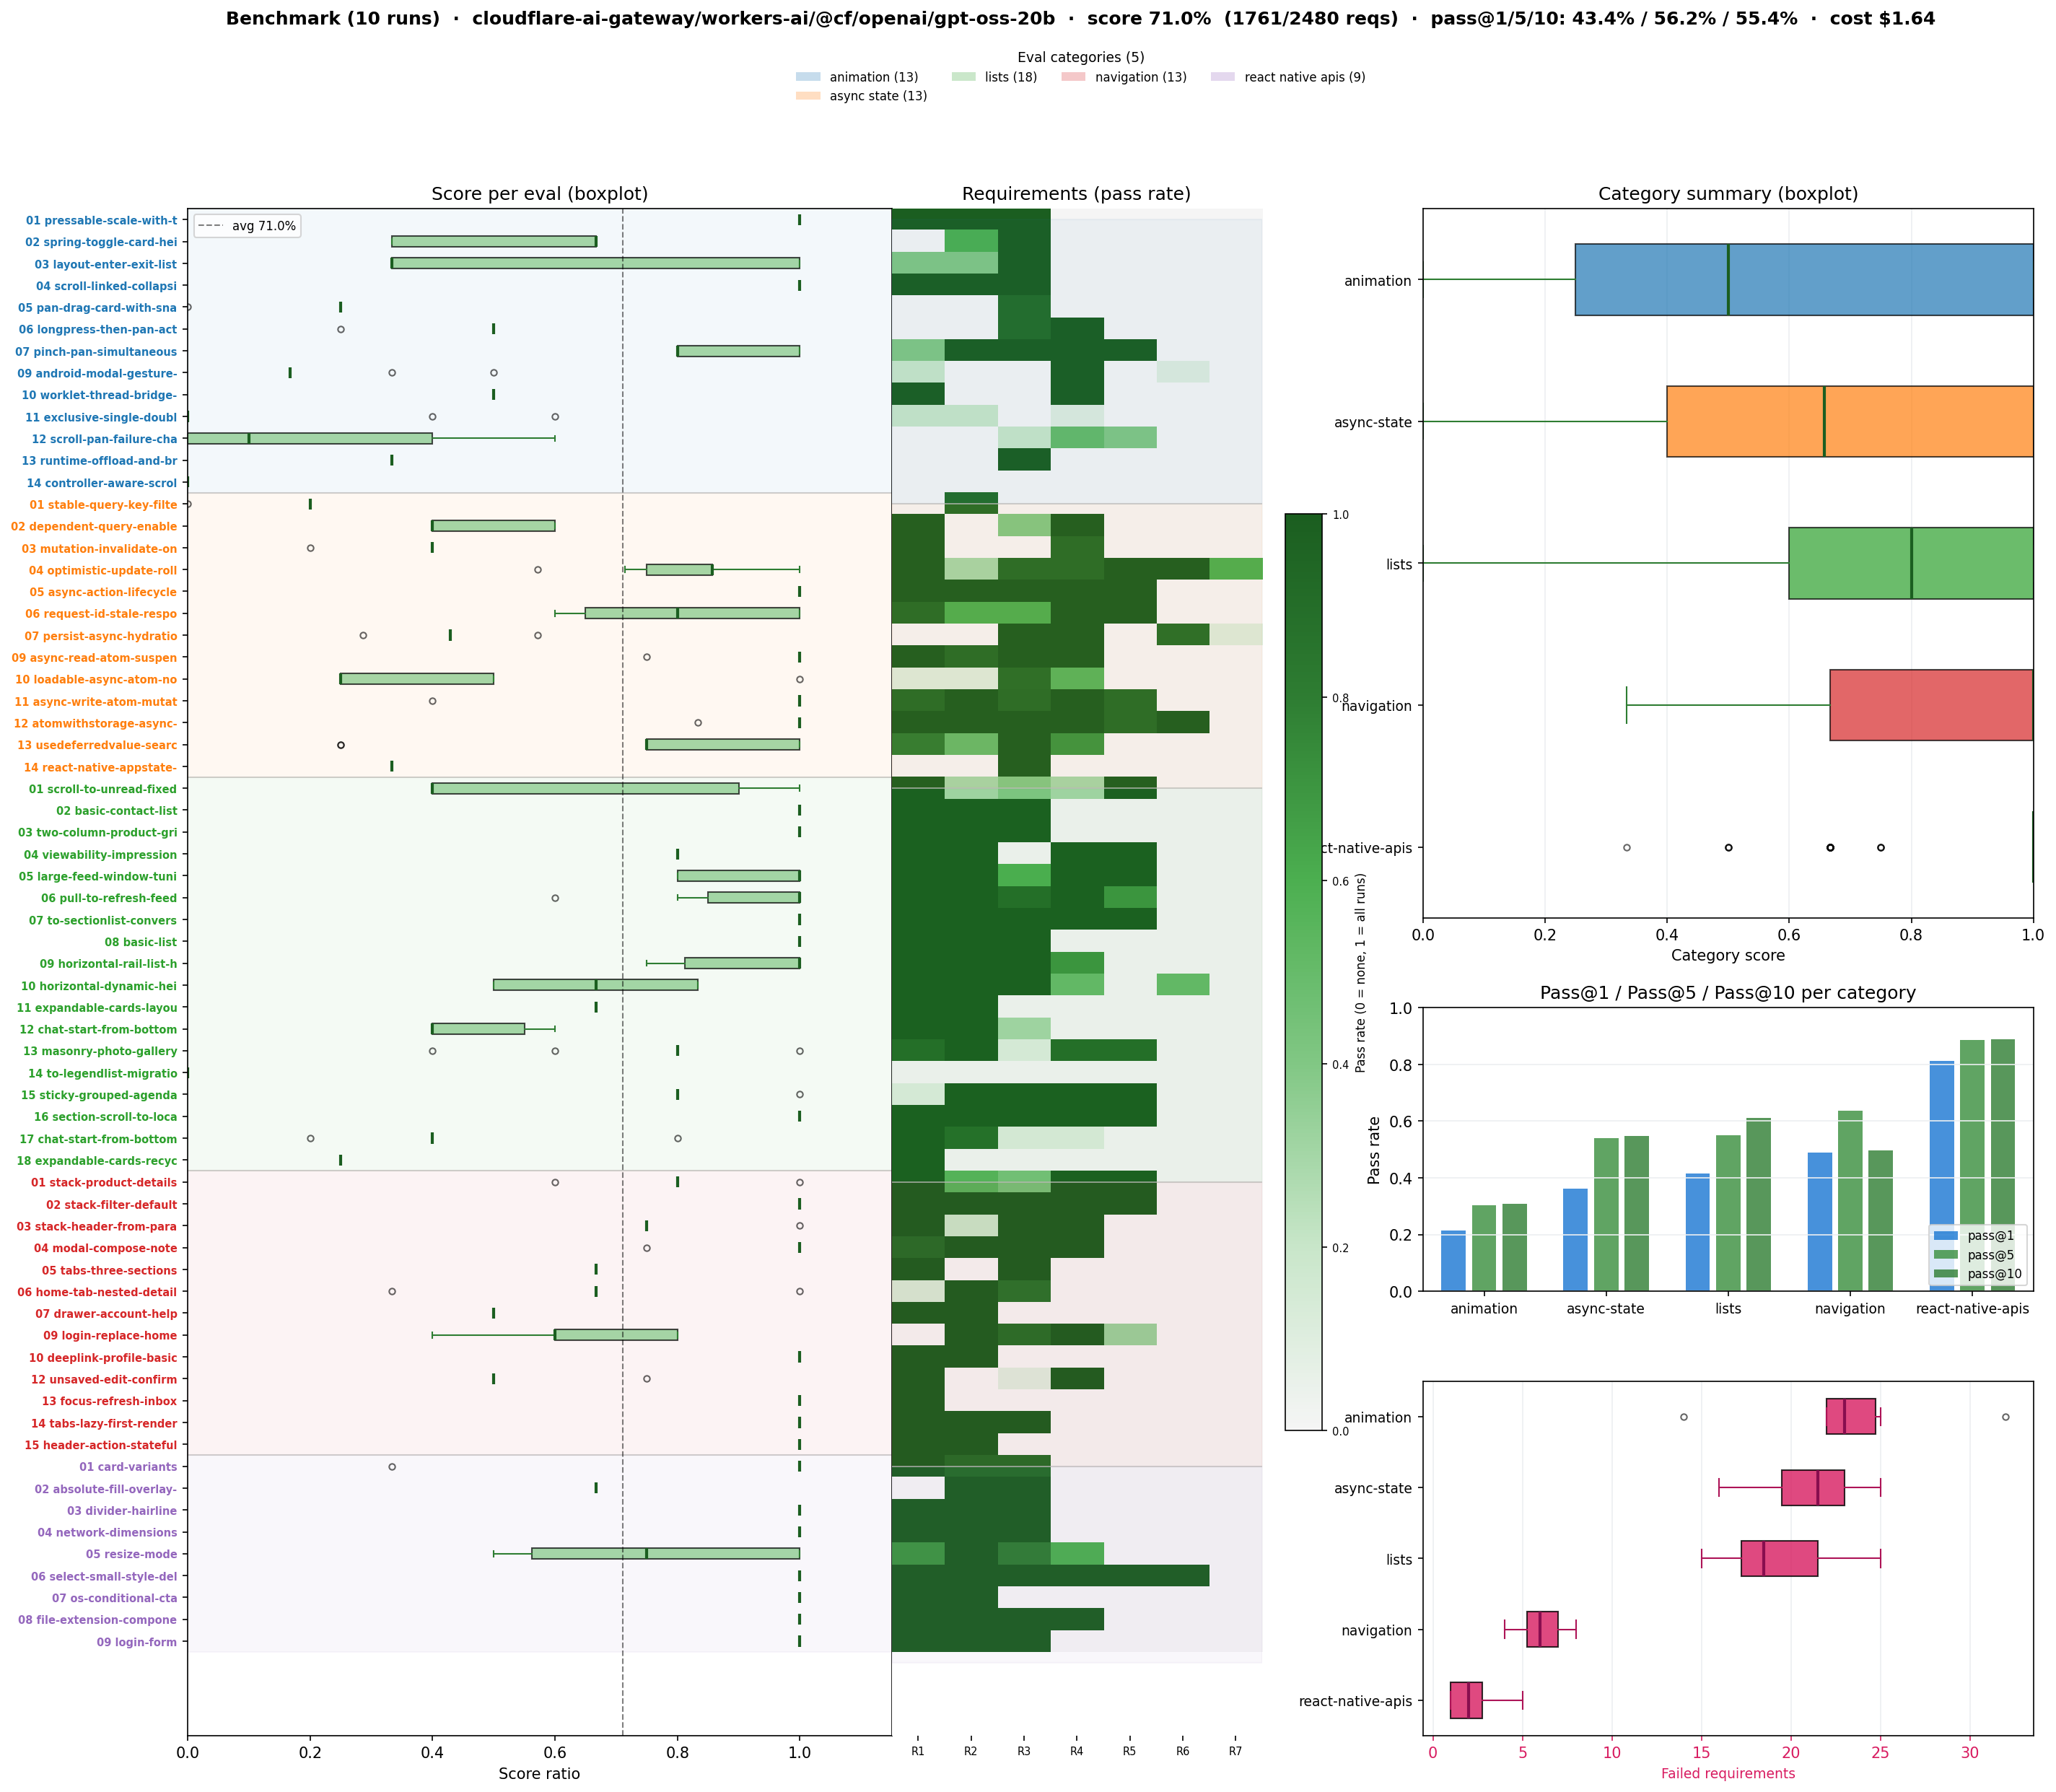
\includegraphics[width=\textwidth]{export/figures/gpt-oss-20b_benchmark_plot.png}
\caption{Benchmark Plot for gpt-oss-20b.}
\end{figure}

\begin{figure}[htbp]
\centering
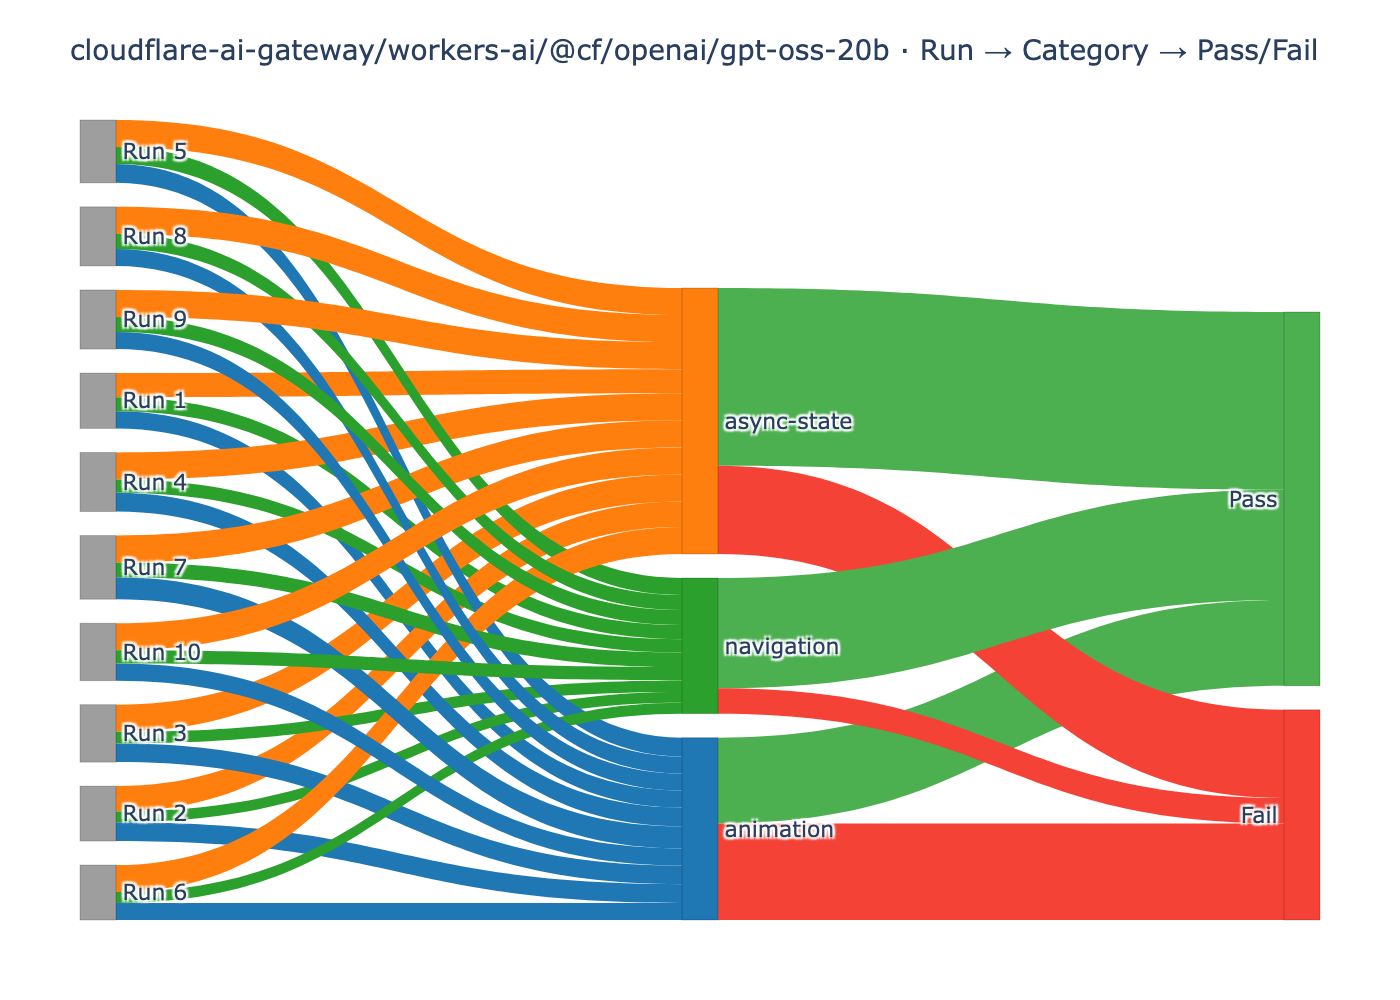
\includegraphics[width=\textwidth]{export/figures/gpt-oss-20b_sankey_per_run.png}
\caption{Sankey per run for gpt-oss-20b showing the distribution of evals with respect to categories and results}
\end{figure}


\clearpage

\subsection{grok-4}

% Table: summary
\input{export/tables/grok-4_summary}

% Table: category_summary
\input{export/tables/grok-4_category_summary}

% Table: per_eval
\input{export/tables/grok-4_per_eval}

\begin{figure}[htbp]
\centering
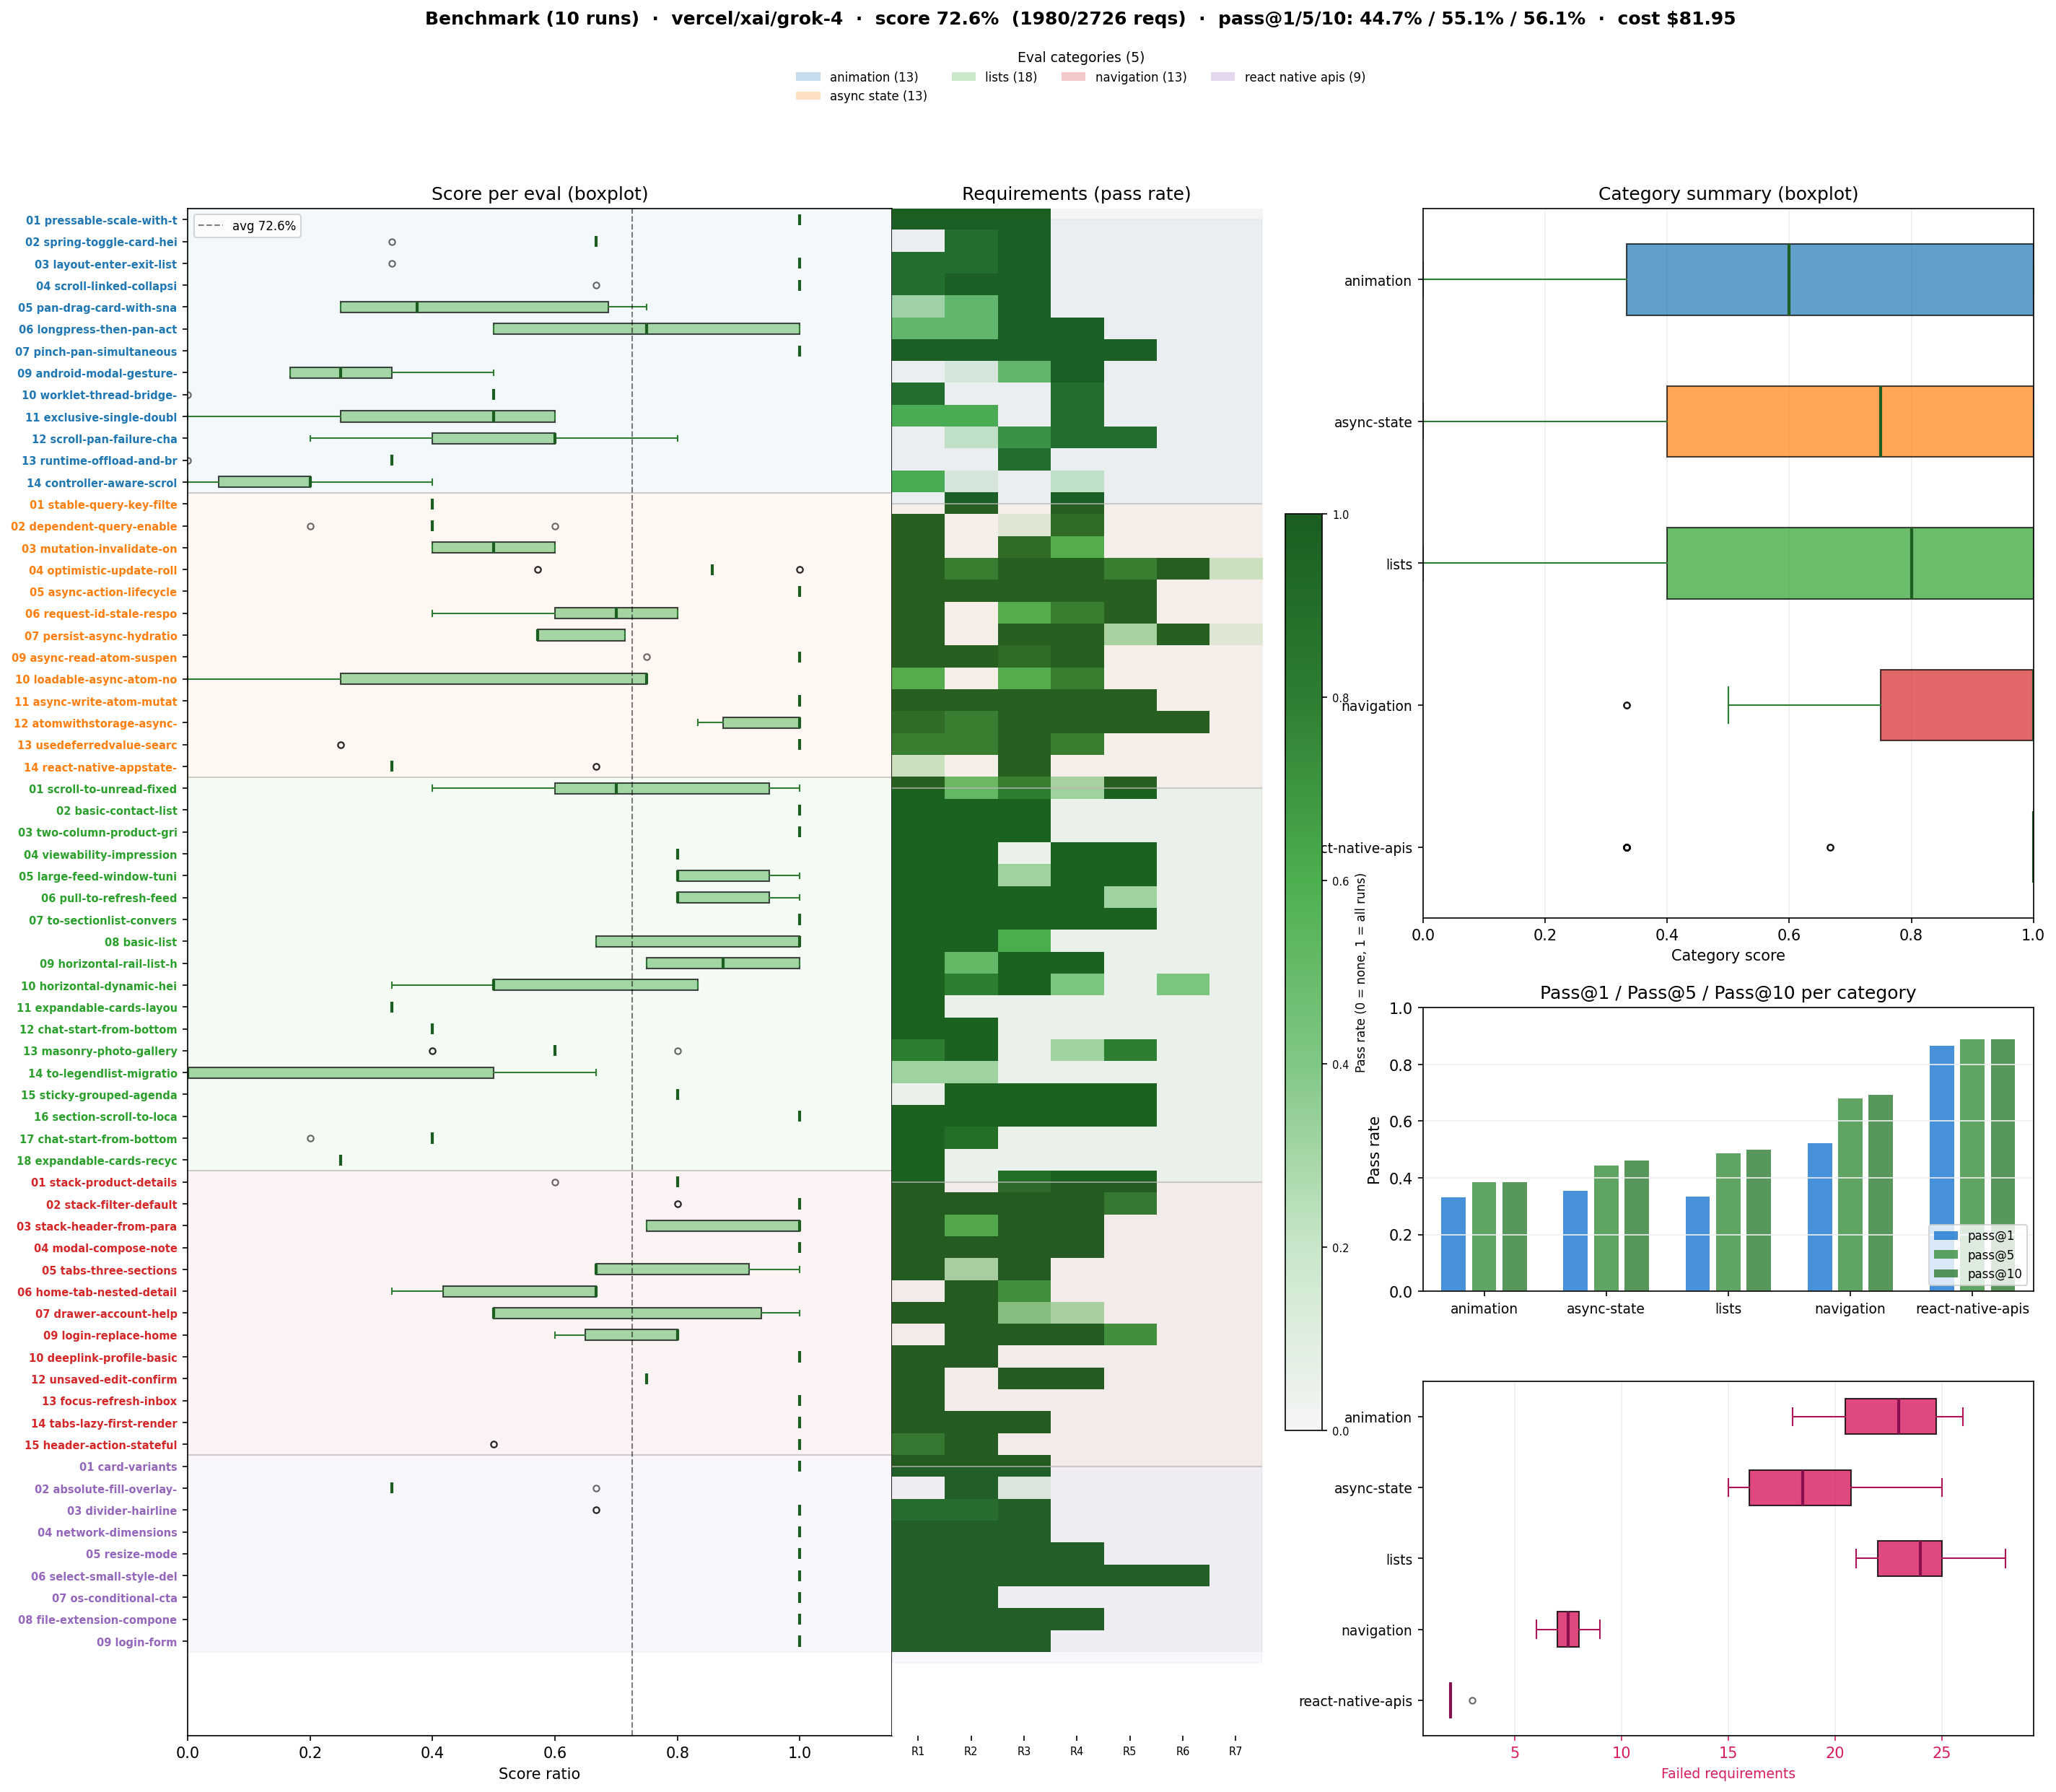
\includegraphics[width=\textwidth]{export/figures/grok-4_benchmark_plot.png}
\caption{Benchmark Plot for grok-4.}
\end{figure}

\begin{figure}[htbp]
\centering
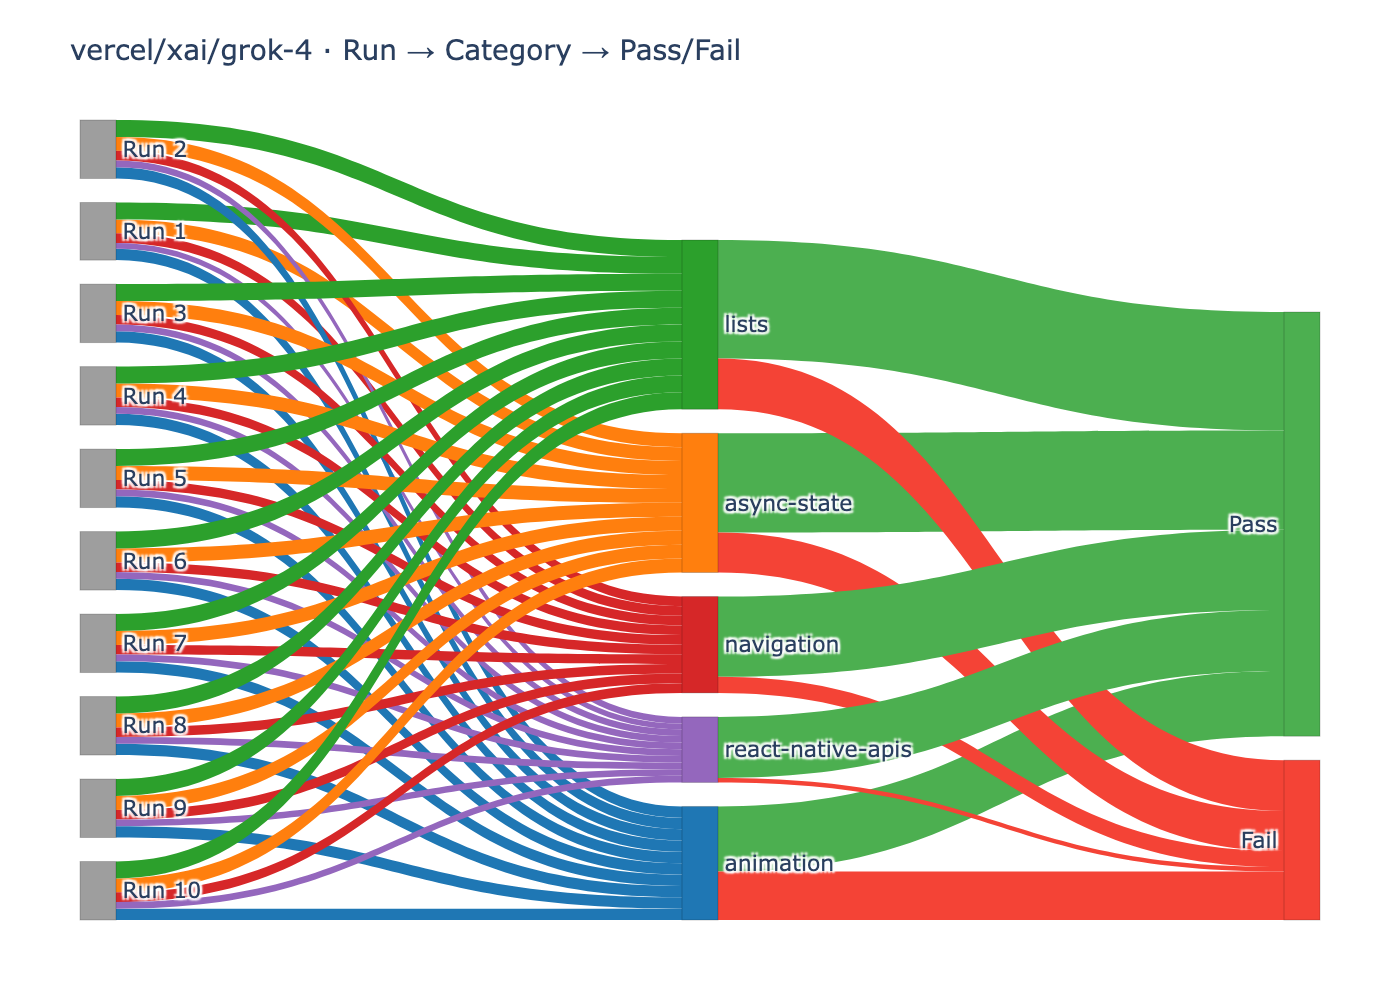
\includegraphics[width=\textwidth]{export/figures/grok-4_sankey_per_run.png}
\caption{Sankey per run for grok-4 showing the distribution of evals with respect to categories and results}
\end{figure}


\clearpage

\subsection{kimi-k2.5}

% Table: summary
\input{export/tables/kimi-k2.5_summary}

% Table: category_summary
\input{export/tables/kimi-k2.5_category_summary}

% Table: per_eval
\input{export/tables/kimi-k2.5_per_eval}

\begin{figure}[htbp]
\centering
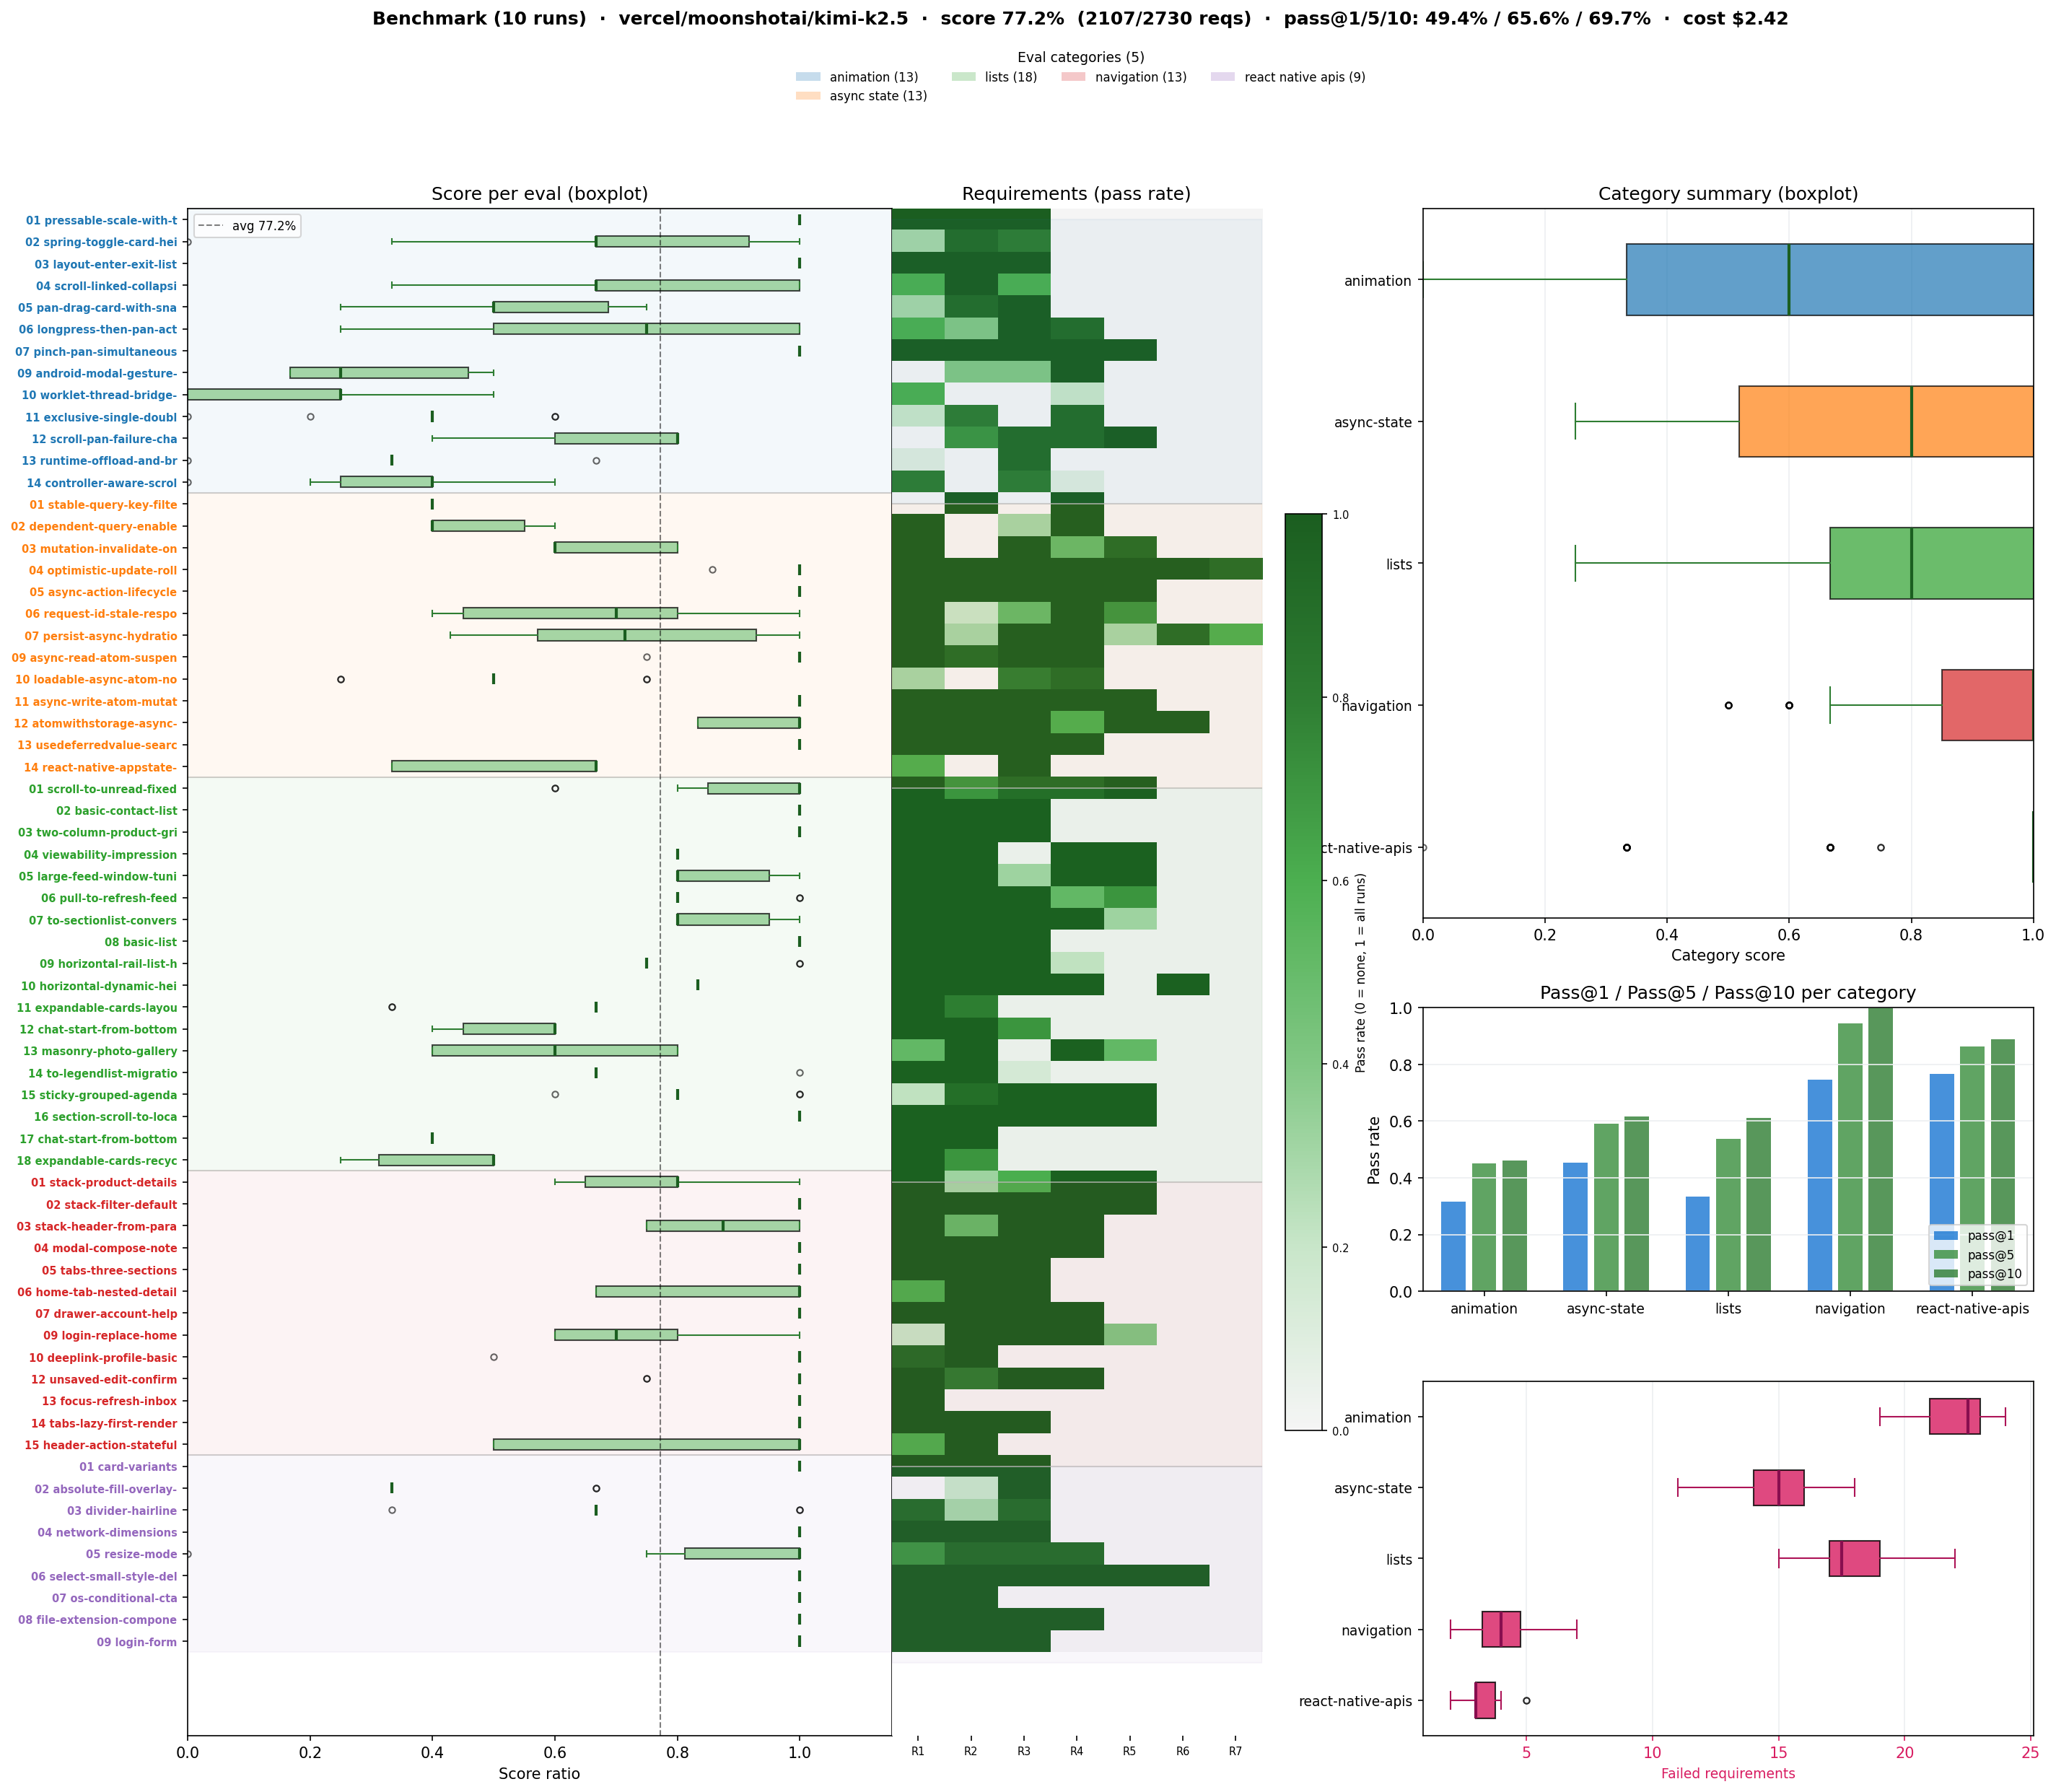
\includegraphics[width=\textwidth]{export/figures/kimi-k2.5_benchmark_plot.png}
\caption{Benchmark Plot for kimi-k2.5.}
\end{figure}

\begin{figure}[htbp]
\centering
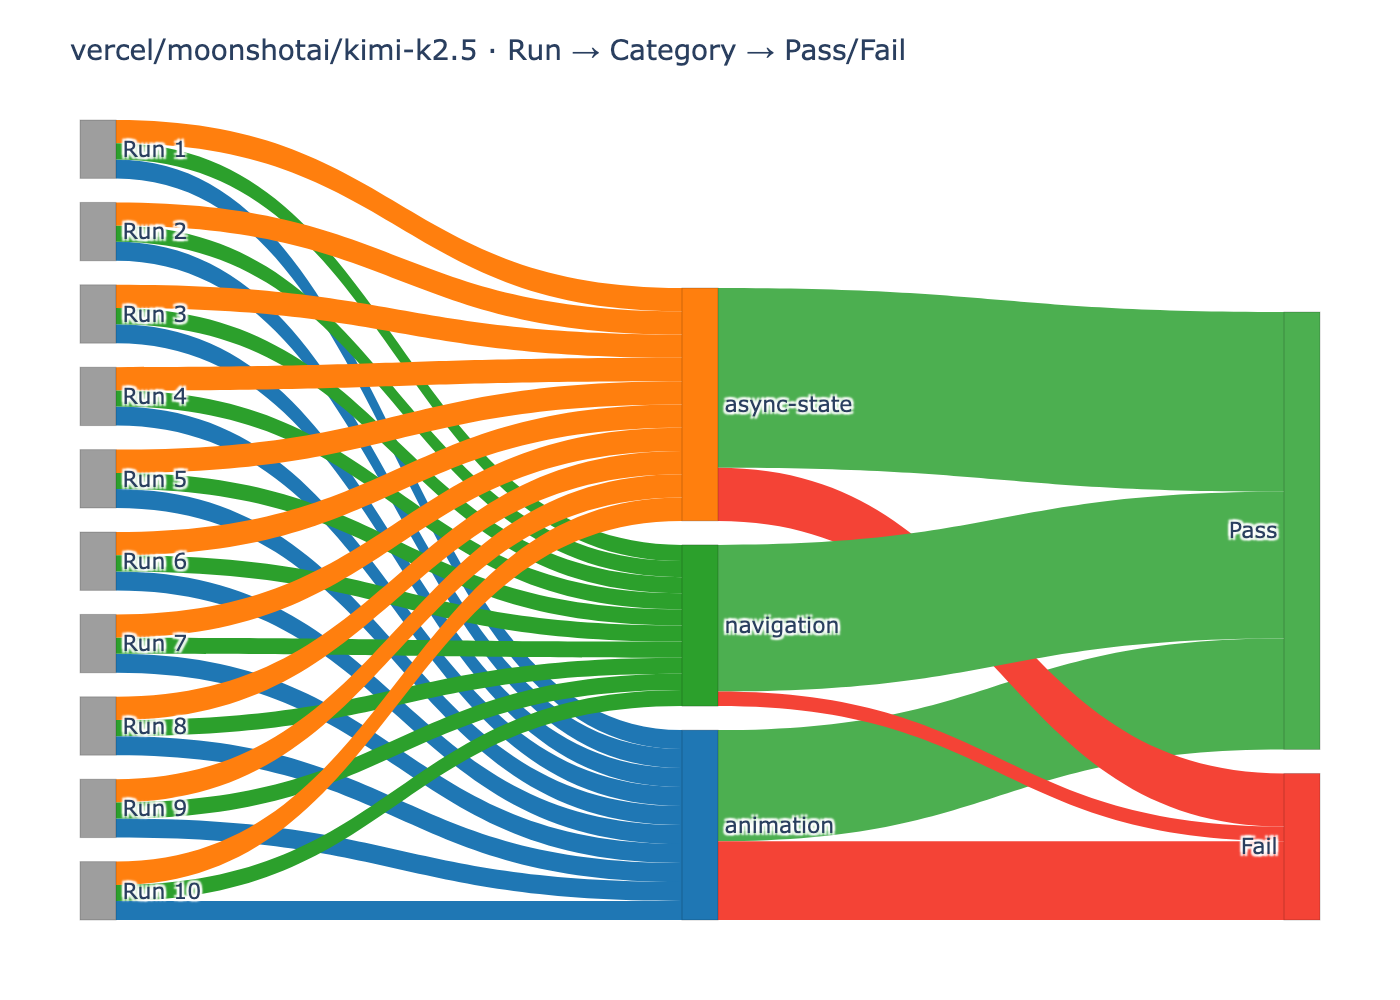
\includegraphics[width=\textwidth]{export/figures/kimi-k2.5_sankey_per_run.png}
\caption{Sankey per run for kimi-k2.5 showing the distribution of evals with respect to categories and results}
\end{figure}


\clearpage

\subsection{qwen2.5-coder-32b-instruct}

% Table: summary
\input{export/tables/qwen2.5-coder-32b-instruct_summary}

% Table: category_summary
\input{export/tables/qwen2.5-coder-32b-instruct_category_summary}

% Table: per_eval
\input{export/tables/qwen2.5-coder-32b-instruct_per_eval}

\begin{figure}[htbp]
\centering
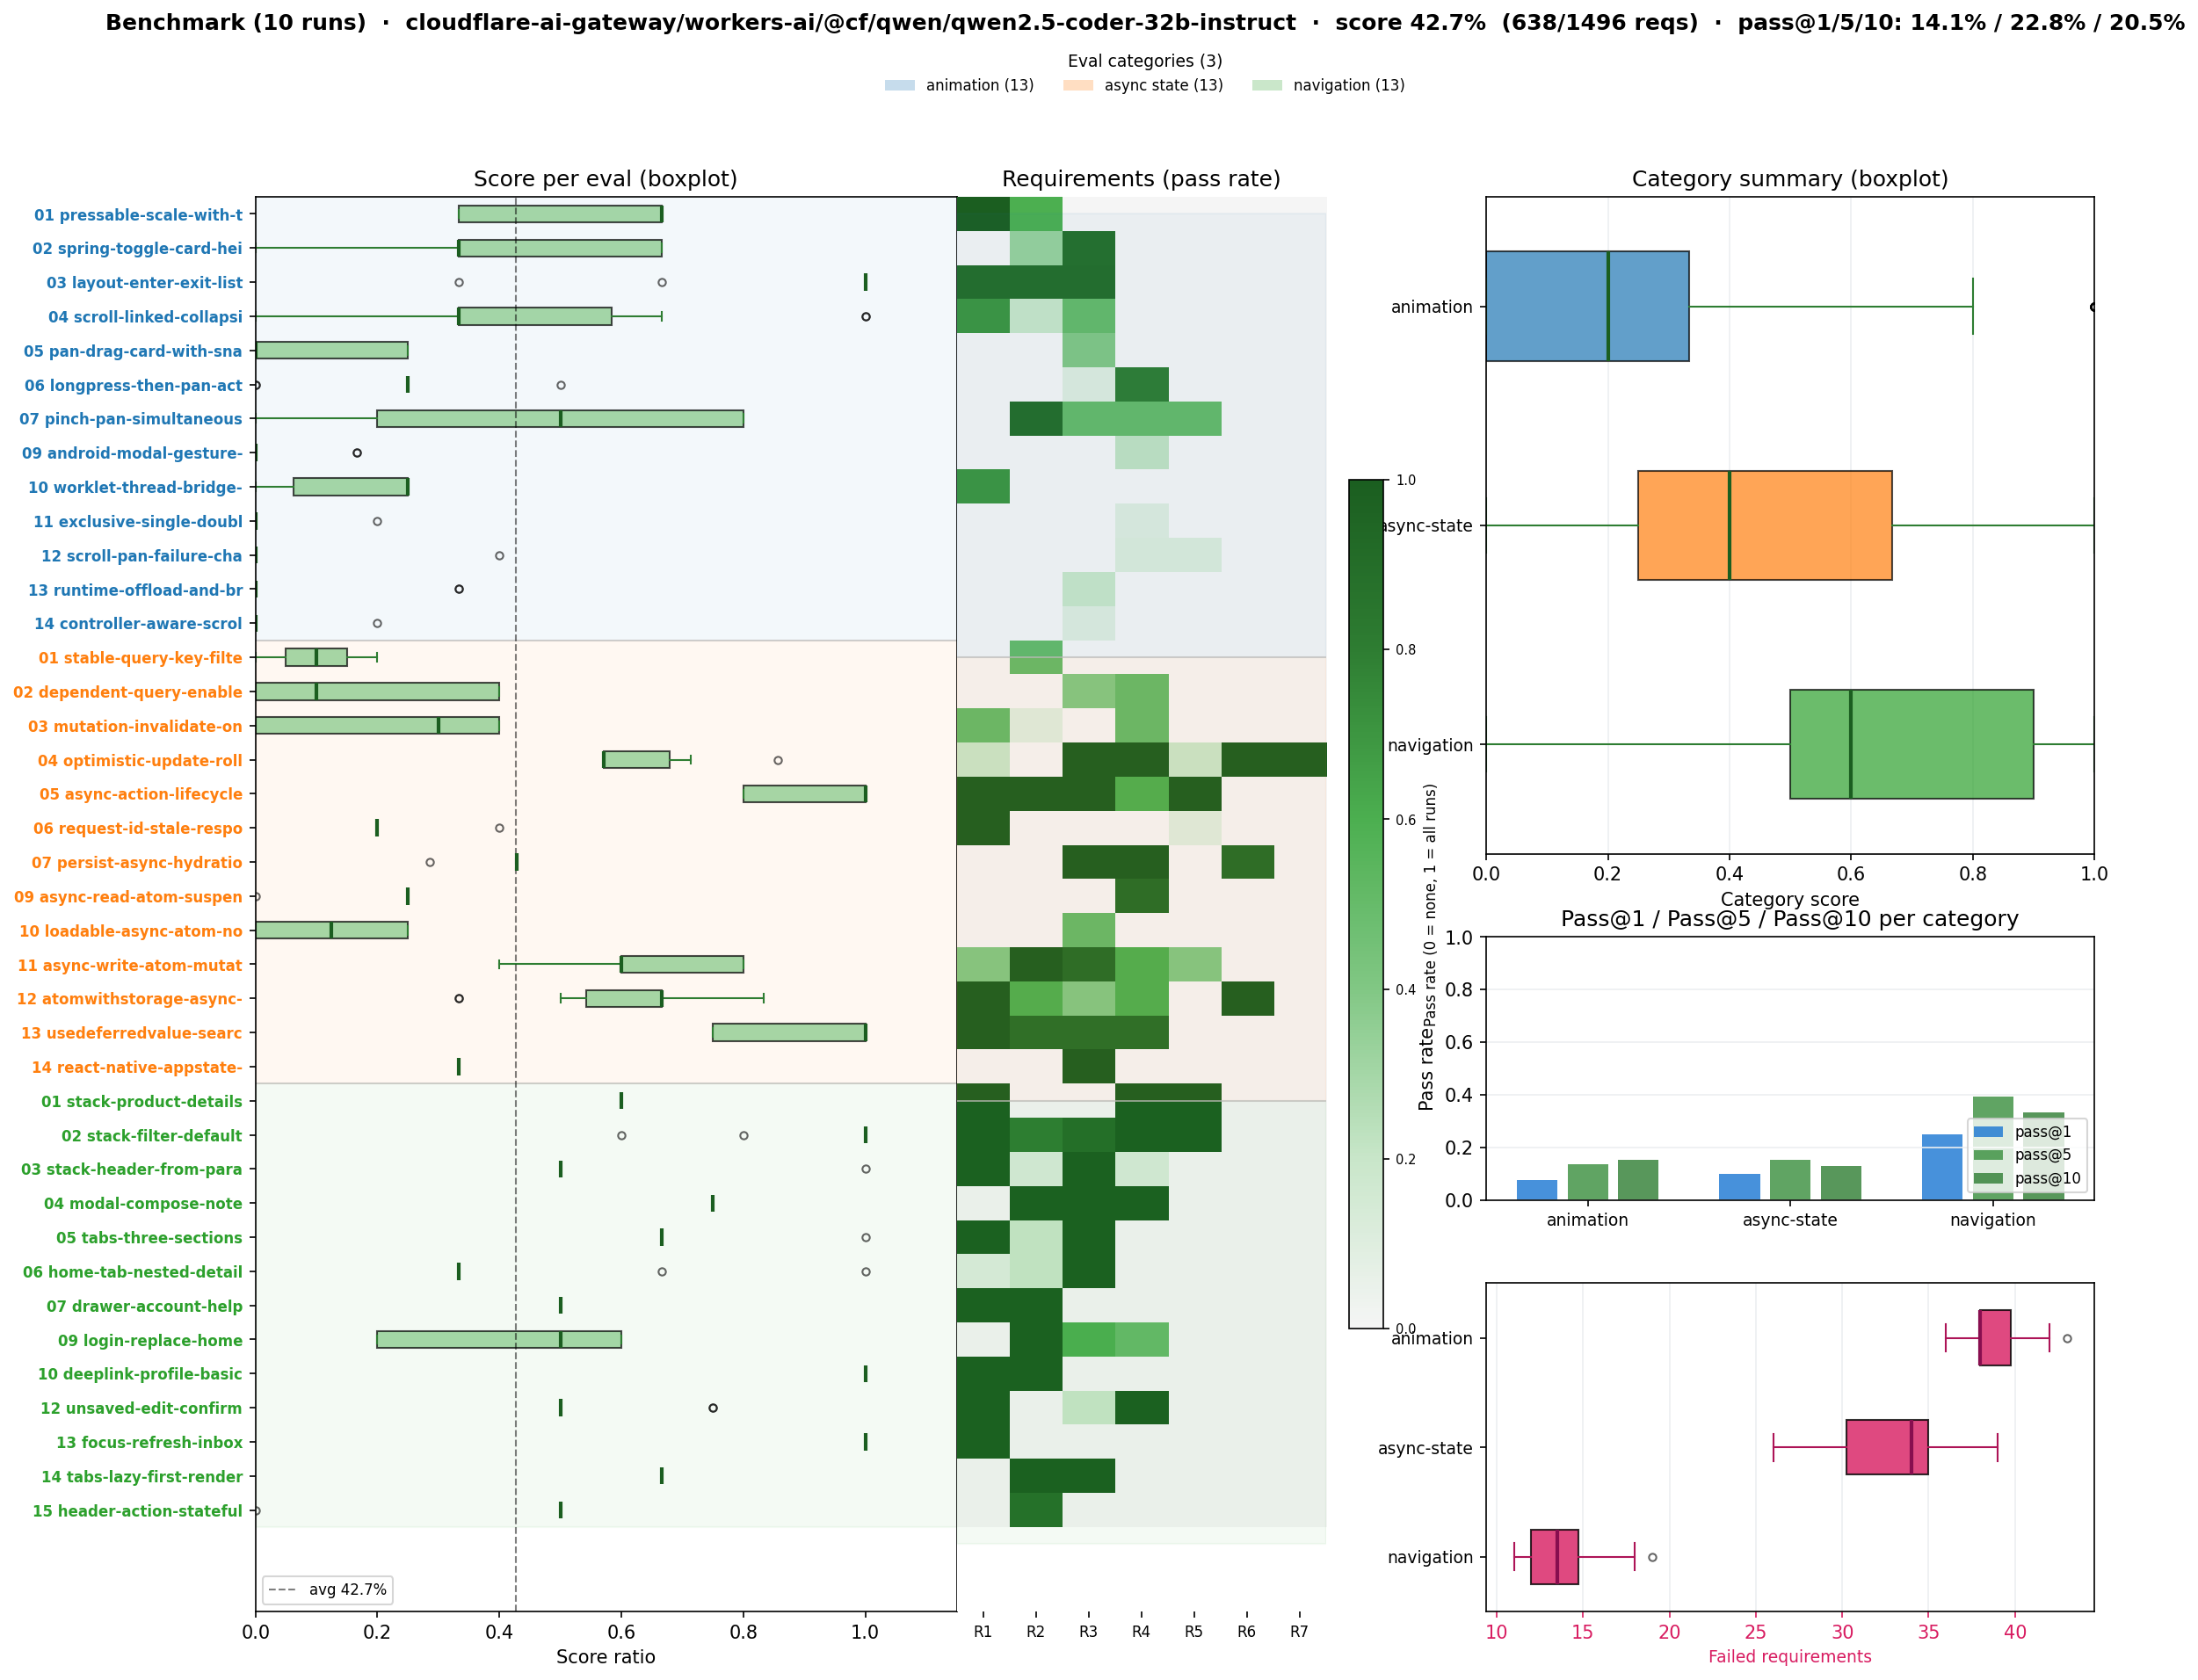
\includegraphics[width=\textwidth]{export/figures/qwen2.5-coder-32b-instruct_benchmark_plot.png}
\caption{Benchmark Plot for qwen2.5-coder-32b-instruct.}
\end{figure}

\begin{figure}[htbp]
\centering
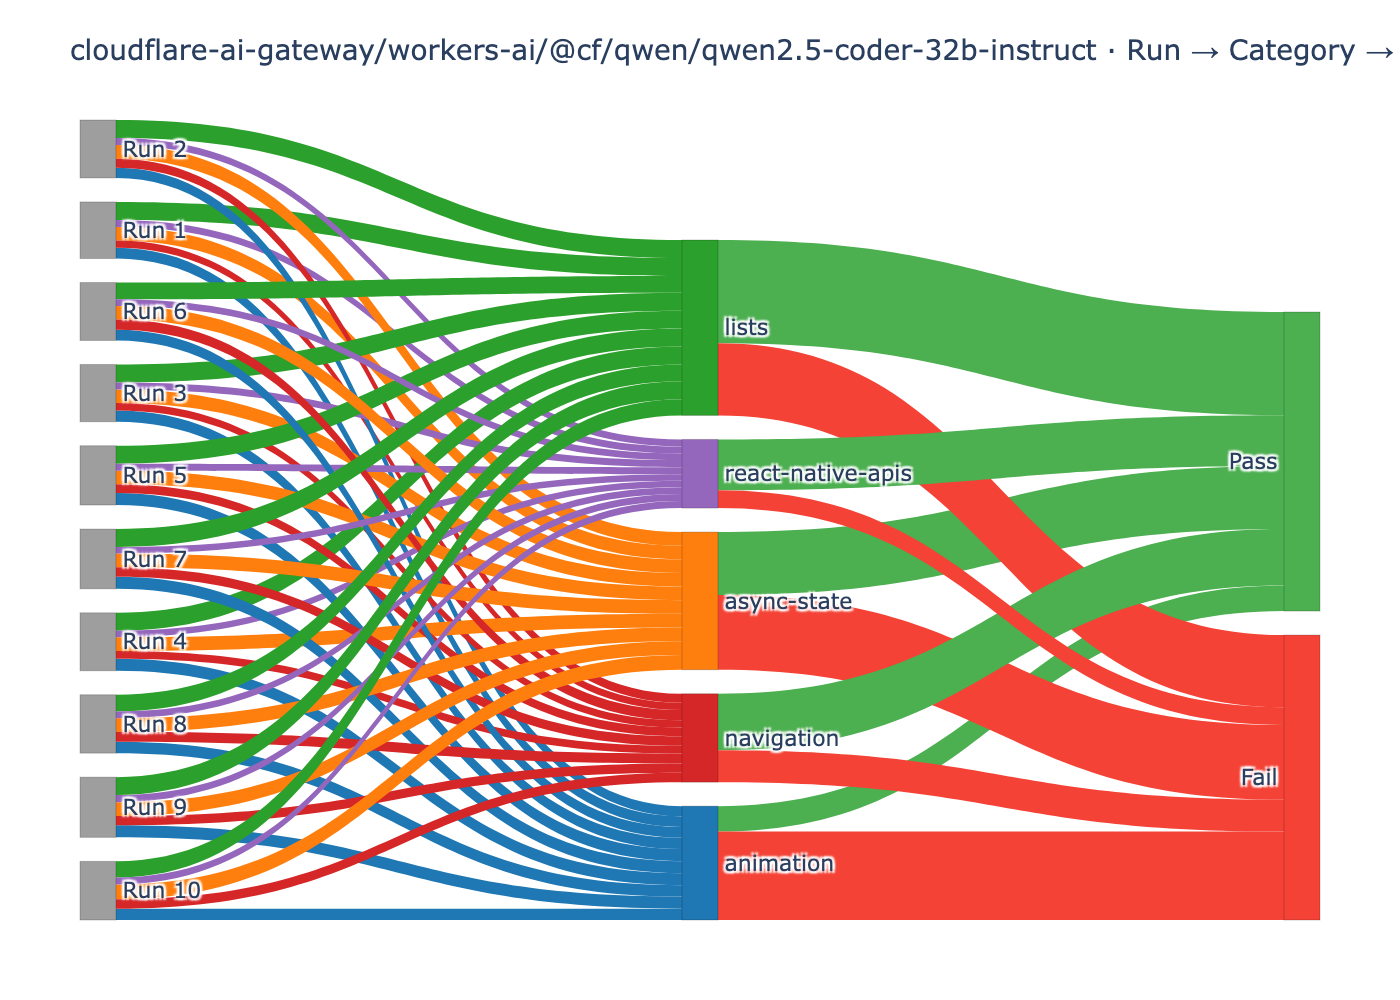
\includegraphics[width=\textwidth]{export/figures/qwen2.5-coder-32b-instruct_sankey_per_run.png}
\caption{Sankey per run for qwen2.5-coder-32b-instruct showing the distribution of evals with respect to categories and results}
\end{figure}
 (compile from repo root)

\appendix
\section{Detailed Results}

\subsection{claude-opus-4.6}

% Table: summary
% Requires: \usepackage{booktabs}
\begin{table}[htbp]
\centering
\begin{tabular}{lrrrrrr}
\toprule
Model & Runs & Score & Reqs & P@1 & P@5 & P@10 \\
\midrule
vercel/anthropic/claude-opus-4.6 & 10 & 84.1\% & 2296/2730 & 60.6\% & 66.8\% & 69.7\% \\
\bottomrule
\end{tabular}
\caption{Model summary for claude-opus-4.6}
\end{table}


% Table: category_summary
% Requires: \usepackage{booktabs}
\begin{table}[htbp]
\centering
\begin{tabular}{lrrrr}
\toprule
Category & Score & Evals & Requirements & Failed requirements \\
\midrule
animation & 77.8\% & 130 & 53 & 121 \\
async state & 83.6\% & 130 & 65 & 106 \\
navigation & 94.5\% & 130 & 45 & 28 \\
\bottomrule
\end{tabular}
\caption{Results by category for claude-opus-4.6. Score: mean(per-eval passed/total weight) across evals and runs. Evals: count of evaluation tasks. Requirements: sum of requirement count per eval. Failed requirements: sum of failed requirement instances across runs.}
\end{table}


% Table: per_eval
% Requires: \usepackage{booktabs}
\begin{table}[htbp]
\centering
\begin{tabular}{lrrrrr}
\toprule
Eval & Category & Score & P@1 & P@5 & P@10 \\
\midrule
01-rn-anim-pressable-scale-with-timing & animation & 100.0\% & 100.0\% & 100.0\% & 100.0\% \\
02-rn-anim-spring-toggle-card-height & animation & 83.3\% & 50.0\% & 99.6\% & 100.0\% \\
03-rn-anim-layout-enter-exit-list-items & animation & 100.0\% & 100.0\% & 100.0\% & 100.0\% \\
04-rn-anim-scroll-linked-collapsing-header & animation & 100.0\% & 100.0\% & 100.0\% & 100.0\% \\
05-rn-anim-pan-drag-card-with-snap-points & animation & 77.5\% & 10.0\% & 50.0\% & 100.0\% \\
06-rn-anim-longpress-then-pan-activation-gate & animation & 100.0\% & 100.0\% & 100.0\% & 100.0\% \\
07-rn-anim-pinch-pan-simultaneous-photo-canvas & animation & 100.0\% & 100.0\% & 100.0\% & 100.0\% \\
09-rn-anim-android-modal-gesture-root-safety & animation & 83.3\% & 0.0\% & 0.0\% & 0.0\% \\
10-rn-anim-worklet-thread-bridge-schedule-on-rn & animation & 37.5\% & 0.0\% & 0.0\% & 0.0\% \\
11-rn-rngh-exclusive-single-double-tap & animation & 62.0\% & 0.0\% & 0.0\% & 0.0\% \\
12-rn-rngh-scroll-pan-failure-chain & animation & 80.0\% & 0.0\% & 0.0\% & 0.0\% \\
13-rn-worklets-runtime-offload-and-bridge & animation & 33.3\% & 0.0\% & 0.0\% & 0.0\% \\
14-rn-keyboard-controller-aware-scroll-footer & animation & 54.0\% & 0.0\% & 0.0\% & 0.0\% \\
01-rn-rq-stable-query-key-filters & async state & 56.0\% & 0.0\% & 0.0\% & 0.0\% \\
02-rn-rq-dependent-query-enabled-gate & async state & 58.0\% & 0.0\% & 0.0\% & 0.0\% \\
03-rn-rq-mutation-invalidate-on-success & async state & 44.0\% & 0.0\% & 0.0\% & 0.0\% \\
04-rn-rq-optimistic-update-rollback & async state & 95.7\% & 70.0\% & 100.0\% & 100.0\% \\
05-rn-zustand-async-action-lifecycle & async state & 100.0\% & 100.0\% & 100.0\% & 100.0\% \\
06-rn-zustand-request-id-stale-response-guard & async state & 76.0\% & 0.0\% & 0.0\% & 0.0\% \\
07-rn-zustand-persist-async-hydration-gate & async state & 88.6\% & 30.0\% & 91.7\% & 100.0\% \\
09-rn-jotai-async-read-atom-suspense & async state & 100.0\% & 100.0\% & 100.0\% & 100.0\% \\
10-rn-jotai-loadable-async-atom-no-suspense & async state & 72.5\% & 20.0\% & 77.8\% & 100.0\% \\
11-rn-jotai-async-write-atom-mutation & async state & 100.0\% & 100.0\% & 100.0\% & 100.0\% \\
12-rn-jotai-atomwithstorage-async-rehydrate-guard & async state & 100.0\% & 100.0\% & 100.0\% & 100.0\% \\
13-rn-react-usedeferredvalue-search-stale-indicator & async state & 100.0\% & 100.0\% & 100.0\% & 100.0\% \\
14-rn-rq-react-native-appstate-focus-online-managers & async state & 96.7\% & 90.0\% & 100.0\% & 100.0\% \\
01-rn-nav-stack-product-details & navigation & 80.0\% & 0.0\% & 0.0\% & 0.0\% \\
02-rn-nav-stack-filter-default & navigation & 100.0\% & 100.0\% & 100.0\% & 100.0\% \\
03-rn-nav-stack-header-from-param & navigation & 75.0\% & 0.0\% & 0.0\% & 0.0\% \\
04-rn-nav-modal-compose-note & navigation & 100.0\% & 100.0\% & 100.0\% & 100.0\% \\
05-rn-nav-tabs-three-sections & navigation & 100.0\% & 100.0\% & 100.0\% & 100.0\% \\
06-rn-nav-home-tab-nested-details & navigation & 73.3\% & 30.0\% & 91.7\% & 100.0\% \\
07-rn-nav-drawer-account-help & navigation & 100.0\% & 100.0\% & 100.0\% & 100.0\% \\
09-rn-nav-login-replace-home & navigation & 100.0\% & 100.0\% & 100.0\% & 100.0\% \\
10-rn-nav-deeplink-profile-basic & navigation & 100.0\% & 100.0\% & 100.0\% & 100.0\% \\
12-rn-nav-unsaved-edit-confirm & navigation & 100.0\% & 100.0\% & 100.0\% & 100.0\% \\
13-rn-nav-focus-refresh-inbox & navigation & 100.0\% & 100.0\% & 100.0\% & 100.0\% \\
14-rn-nav-tabs-lazy-first-render & navigation & 100.0\% & 100.0\% & 100.0\% & 100.0\% \\
15-rn-nav-header-action-stateful & navigation & 100.0\% & 100.0\% & 100.0\% & 100.0\% \\
\bottomrule
\end{tabular}
\caption{Per-eval results (score and pass@k) for claude-opus-4.6}
\end{table}


\begin{figure}[htbp]
\centering
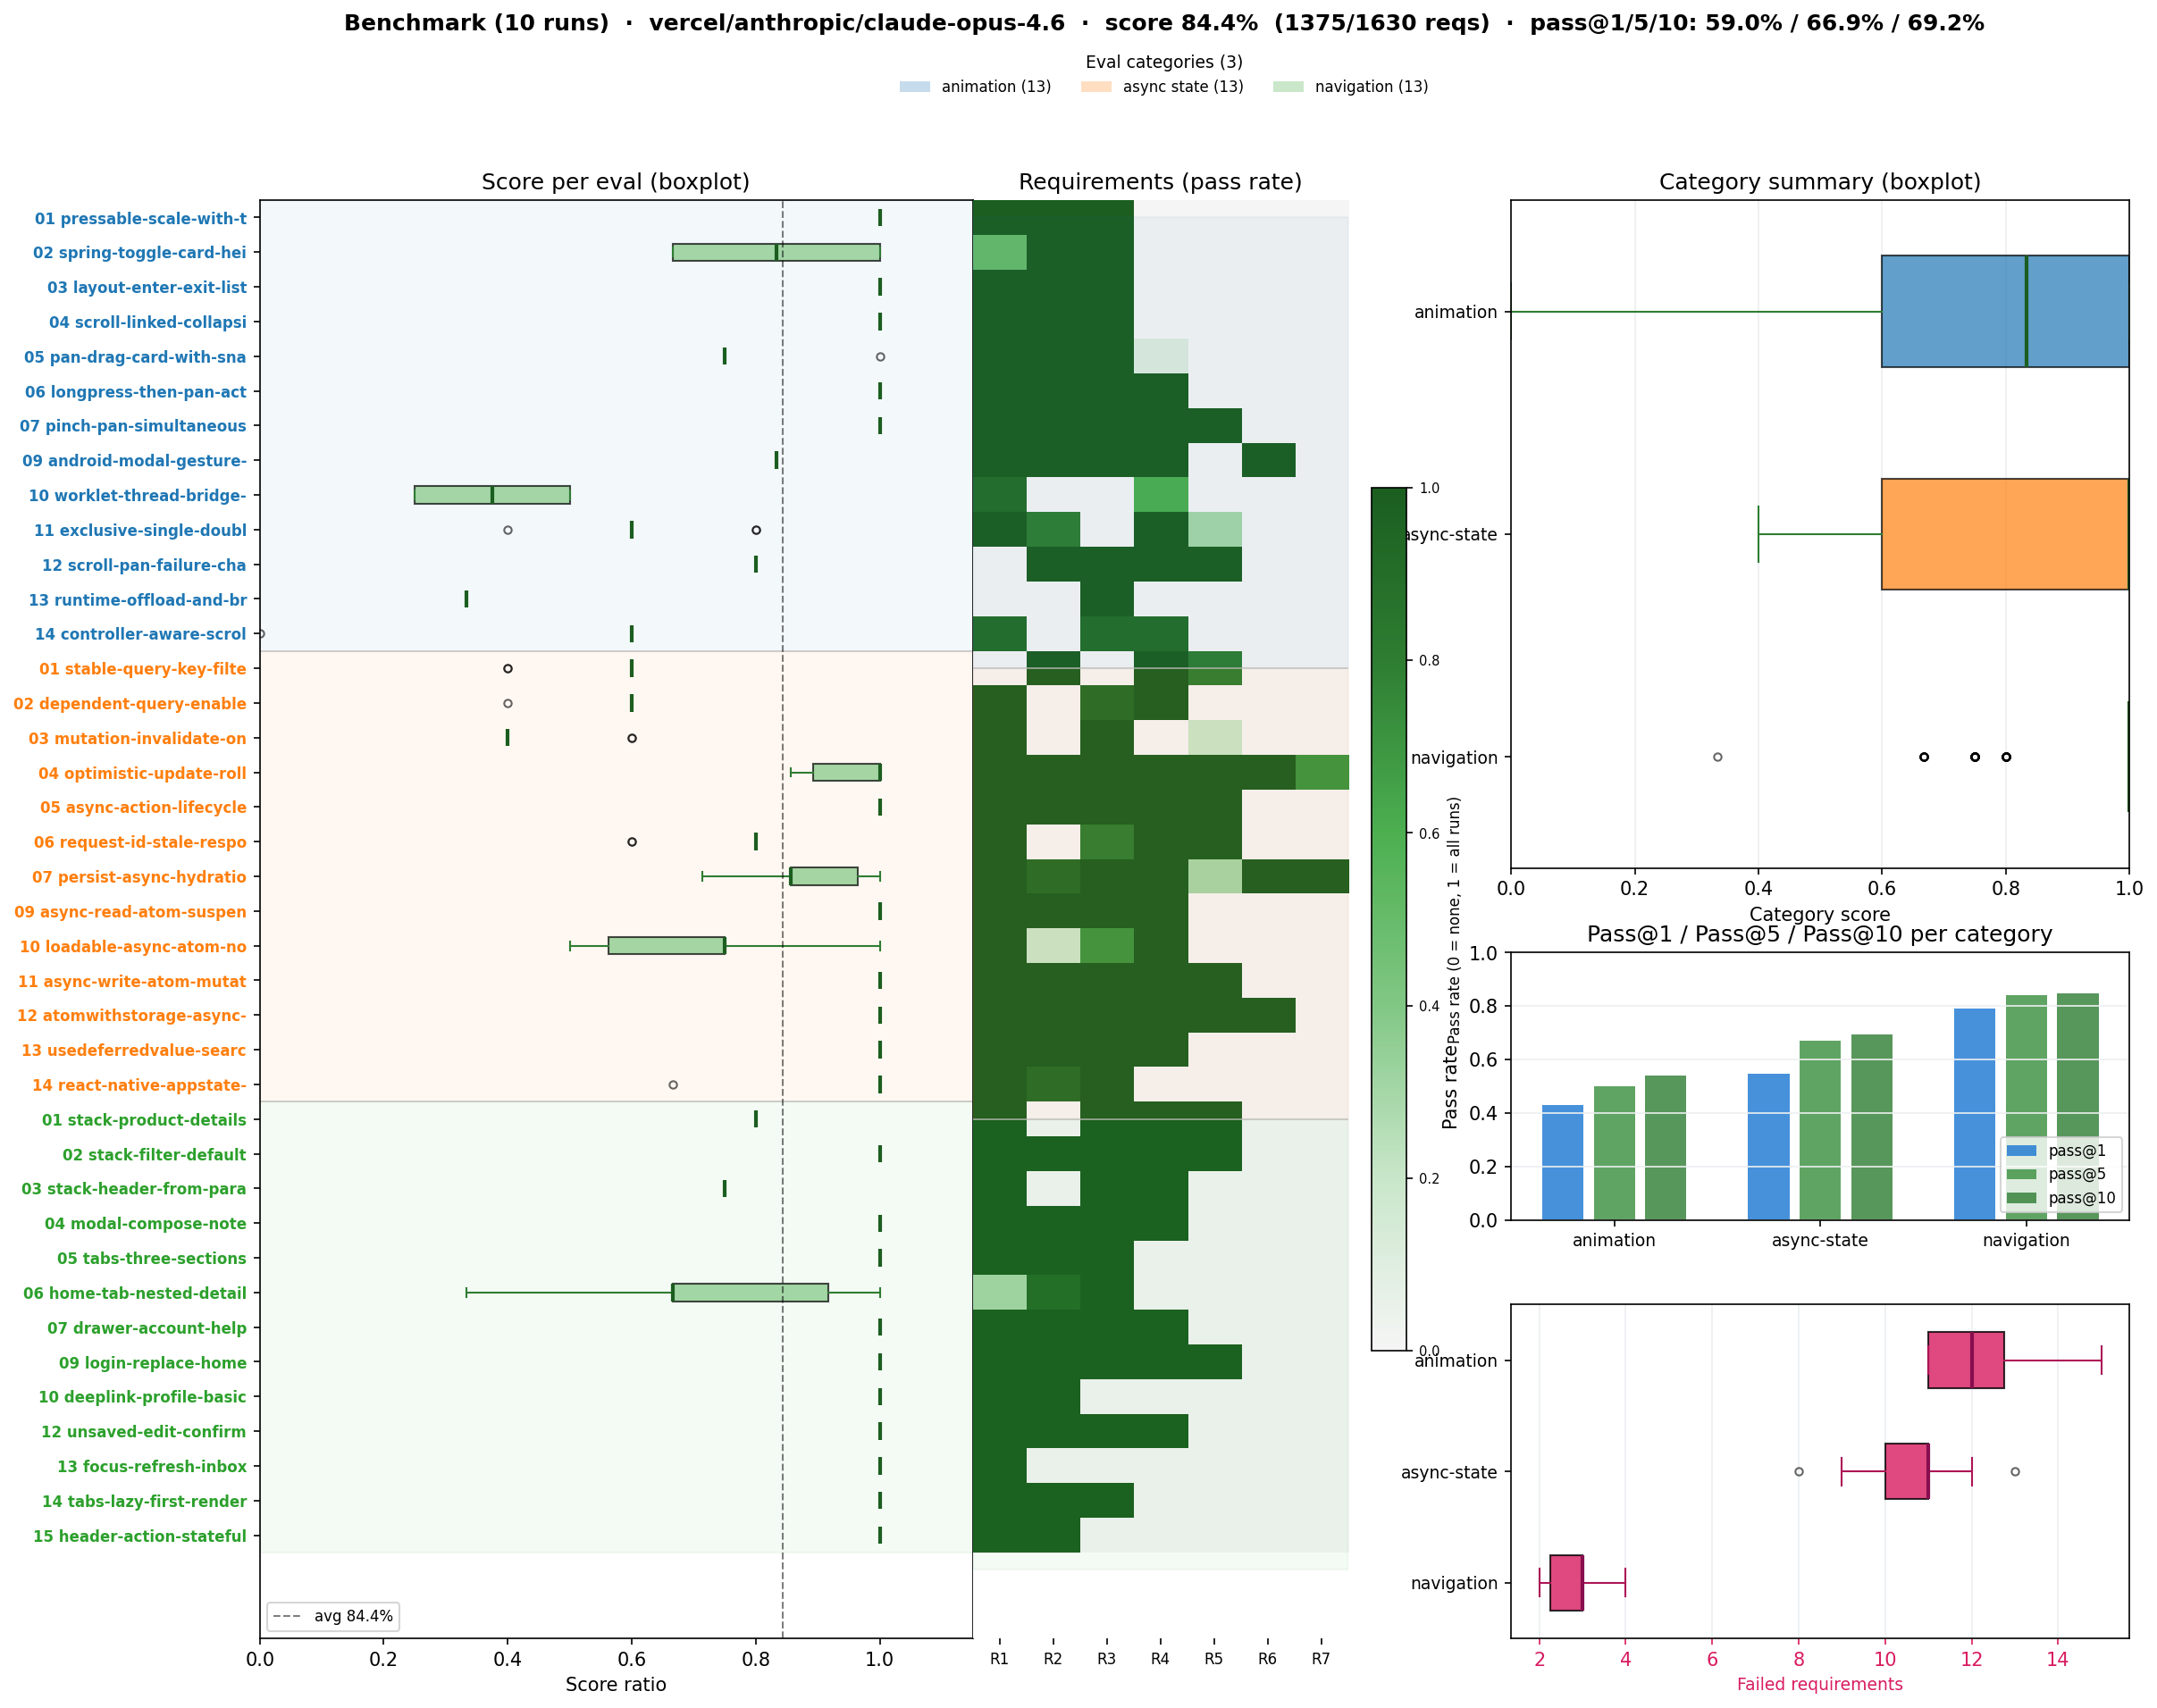
\includegraphics[width=\textwidth]{export/figures/claude-opus-4.6_benchmark_plot.png}
\caption{Benchmark Plot for claude-opus-4.6.}
\end{figure}

\begin{figure}[htbp]
\centering
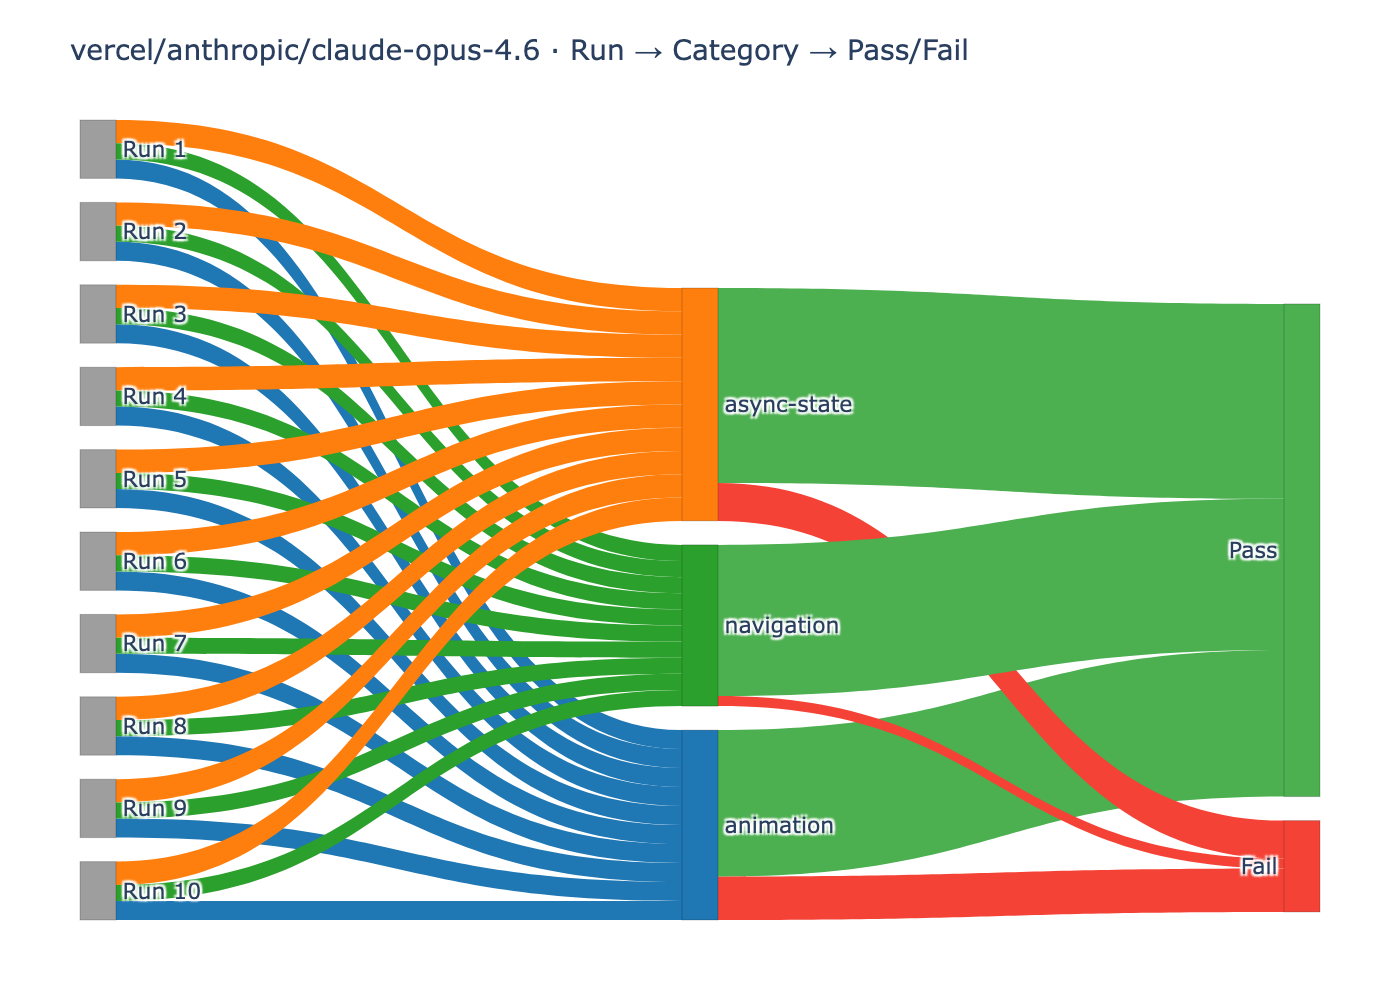
\includegraphics[width=\textwidth]{export/figures/claude-opus-4.6_sankey_per_run.png}
\caption{Sankey per run for claude-opus-4.6 showing the distribution of evals with respect to categories and results}
\end{figure}


\clearpage

\subsection{claude-sonnet-4.6}

% Table: summary
% Requires: \usepackage{booktabs}
\begin{table}[htbp]
\centering
\begin{tabular}{lrrrrrr}
\toprule
Model & Runs & Score & Reqs & P@1 & P@5 & P@10 \\
\midrule
vercel/anthropic/claude-sonnet-4.6 & 10 & 80.6\% & 2201/2730 & 55.0\% & 63.4\% & 66.7\% \\
\bottomrule
\end{tabular}
\caption{Model summary for claude-sonnet-4.6}
\end{table}


% Table: category_summary
% Requires: \usepackage{booktabs}
\begin{table}[htbp]
\centering
\begin{tabular}{lrrrr}
\toprule
Category & Score & Evals & Requirements & Failed requirements \\
\midrule
animation & 66.9\% & 130 & 53 & 191 \\
async state & 76.9\% & 130 & 65 & 139 \\
lists & 80.4\% & 180 & 79 & 151 \\
navigation & 93.8\% & 130 & 45 & 30 \\
react native apis & 93.3\% & 90 & 31 & 18 \\
\bottomrule
\end{tabular}
\caption{Results by category for claude-sonnet-4.6. Score: mean(per-eval passed/total weight) across evals and runs. Evals: count of evaluation tasks. Requirements: sum of requirement count per eval. Failed requirements: sum of failed requirement instances across runs.}
\end{table}


% Table: per_eval
% Requires: \usepackage{booktabs}
\begin{table}[htbp]
\centering
\begin{adjustbox}{width=0.8\textwidth}
\begin{tabular}{lrrrrr}
\toprule
Eval & Category & Score & P@1 & P@5 & P@10 \\
\midrule
01-rn-anim-pressable-scale-with-timing & animation & 100.0\% & 100.0\% & 100.0\% & 100.0\% \\
02-rn-anim-spring-toggle-card-height & animation & 80.0\% & 50.0\% & 99.6\% & 100.0\% \\
03-rn-anim-layout-enter-exit-list-items & animation & 100.0\% & 100.0\% & 100.0\% & 100.0\% \\
04-rn-anim-scroll-linked-collapsing-header & animation & 86.7\% & 60.0\% & 100.0\% & 100.0\% \\
05-rn-anim-pan-drag-card-with-snap-points & animation & 70.0\% & 0.0\% & 0.0\% & 0.0\% \\
06-rn-anim-longpress-then-pan-activation-gate & animation & 87.5\% & 50.0\% & 99.6\% & 100.0\% \\
07-rn-anim-pinch-pan-simultaneous-photo-canvas & animation & 100.0\% & 100.0\% & 100.0\% & 100.0\% \\
09-rn-anim-android-modal-gesture-root-safety & animation & 40.0\% & 0.0\% & 0.0\% & 0.0\% \\
10-rn-anim-worklet-thread-bridge-schedule-on-rn & animation & 40.0\% & 0.0\% & 0.0\% & 0.0\% \\
11-rn-rngh-exclusive-single-double-tap & animation & 54.0\% & 0.0\% & 0.0\% & 0.0\% \\
12-rn-rngh-scroll-pan-failure-chain & animation & 52.0\% & 0.0\% & 0.0\% & 0.0\% \\
13-rn-worklets-runtime-offload-and-bridge & animation & 33.3\% & 0.0\% & 0.0\% & 0.0\% \\
14-rn-keyboard-controller-aware-scroll-footer & animation & 26.0\% & 0.0\% & 0.0\% & 0.0\% \\
01-rn-rq-stable-query-key-filters & async state & 46.0\% & 0.0\% & 0.0\% & 0.0\% \\
02-rn-rq-dependent-query-enabled-gate & async state & 36.0\% & 0.0\% & 0.0\% & 0.0\% \\
03-rn-rq-mutation-invalidate-on-success & async state & 72.0\% & 0.0\% & 0.0\% & 0.0\% \\
04-rn-rq-optimistic-update-rollback & async state & 95.7\% & 90.0\% & 100.0\% & 100.0\% \\
05-rn-zustand-async-action-lifecycle & async state & 100.0\% & 100.0\% & 100.0\% & 100.0\% \\
06-rn-zustand-request-id-stale-response-guard & async state & 80.0\% & 0.0\% & 0.0\% & 0.0\% \\
07-rn-zustand-persist-async-hydration-gate & async state & 80.0\% & 10.0\% & 50.0\% & 100.0\% \\
09-rn-jotai-async-read-atom-suspense & async state & 90.0\% & 80.0\% & 100.0\% & 100.0\% \\
10-rn-jotai-loadable-async-atom-no-suspense & async state & 65.0\% & 0.0\% & 0.0\% & 0.0\% \\
11-rn-jotai-async-write-atom-mutation & async state & 100.0\% & 100.0\% & 100.0\% & 100.0\% \\
12-rn-jotai-atomwithstorage-async-rehydrate-guard & async state & 95.0\% & 70.0\% & 100.0\% & 100.0\% \\
13-rn-react-usedeferredvalue-search-stale-indicator & async state & 100.0\% & 100.0\% & 100.0\% & 100.0\% \\
14-rn-rq-react-native-appstate-focus-online-managers & async state & 40.0\% & 0.0\% & 0.0\% & 0.0\% \\
01-rn-flatlist-scroll-to-unread-fixed-rows & lists & 92.0\% & 80.0\% & 100.0\% & 100.0\% \\
02-rn-flatlist-basic-contact-list & lists & 100.0\% & 100.0\% & 100.0\% & 100.0\% \\
03-rn-flatlist-two-column-product-grid & lists & 100.0\% & 100.0\% & 100.0\% & 100.0\% \\
04-rn-flatlist-viewability-impression-tracking & lists & 80.0\% & 0.0\% & 0.0\% & 0.0\% \\
05-rn-flatlist-large-feed-window-tuning & lists & 100.0\% & 100.0\% & 100.0\% & 100.0\% \\
06-rn-flatlist-pull-to-refresh-feed & lists & 100.0\% & 100.0\% & 100.0\% & 100.0\% \\
07-rn-flatlist-to-sectionlist-conversion & lists & 100.0\% & 100.0\% & 100.0\% & 100.0\% \\
08-rn-flashlist-basic-list & lists & 100.0\% & 100.0\% & 100.0\% & 100.0\% \\
09-rn-flashlist-horizontal-rail-list-header & lists & 82.5\% & 30.0\% & 91.7\% & 100.0\% \\
10-rn-flashlist-horizontal-dynamic-height-header-first-item & lists & 88.3\% & 30.0\% & 91.7\% & 100.0\% \\
11-rn-flashlist-expandable-cards-layout-state & lists & 53.3\% & 0.0\% & 0.0\% & 0.0\% \\
12-rn-flashlist-chat-start-from-bottom & lists & 40.0\% & 0.0\% & 0.0\% & 0.0\% \\
13-rn-flashlist-masonry-photo-gallery & lists & 54.0\% & 0.0\% & 0.0\% & 0.0\% \\
14-rn-flatlist-to-legendlist-migration & lists & 46.7\% & 0.0\% & 0.0\% & 0.0\% \\
15-rn-legendlist-sticky-grouped-agenda & lists & 80.0\% & 0.0\% & 0.0\% & 0.0\% \\
16-rn-legendlist-section-scroll-to-location & lists & 100.0\% & 100.0\% & 100.0\% & 100.0\% \\
17-rn-legendlist-chat-start-from-bottom & lists & 80.0\% & 0.0\% & 0.0\% & 0.0\% \\
18-rn-legendlist-expandable-cards-recycling-state & lists & 50.0\% & 0.0\% & 0.0\% & 0.0\% \\
01-rn-nav-stack-product-details & navigation & 82.0\% & 10.0\% & 50.0\% & 100.0\% \\
02-rn-nav-stack-filter-default & navigation & 100.0\% & 100.0\% & 100.0\% & 100.0\% \\
03-rn-nav-stack-header-from-param & navigation & 77.5\% & 10.0\% & 50.0\% & 100.0\% \\
04-rn-nav-modal-compose-note & navigation & 100.0\% & 100.0\% & 100.0\% & 100.0\% \\
05-rn-nav-tabs-three-sections & navigation & 100.0\% & 100.0\% & 100.0\% & 100.0\% \\
06-rn-nav-home-tab-nested-details & navigation & 70.0\% & 10.0\% & 50.0\% & 100.0\% \\
07-rn-nav-drawer-account-help & navigation & 100.0\% & 100.0\% & 100.0\% & 100.0\% \\
09-rn-nav-login-replace-home & navigation & 100.0\% & 100.0\% & 100.0\% & 100.0\% \\
10-rn-nav-deeplink-profile-basic & navigation & 100.0\% & 100.0\% & 100.0\% & 100.0\% \\
12-rn-nav-unsaved-edit-confirm & navigation & 95.0\% & 80.0\% & 100.0\% & 100.0\% \\
13-rn-nav-focus-refresh-inbox & navigation & 100.0\% & 100.0\% & 100.0\% & 100.0\% \\
14-rn-nav-tabs-lazy-first-render & navigation & 100.0\% & 100.0\% & 100.0\% & 100.0\% \\
15-rn-nav-header-action-stateful & navigation & 95.0\% & 90.0\% & 100.0\% & 100.0\% \\
01-rn-stylesheet-card-variants & react native apis & 100.0\% & 100.0\% & 100.0\% & 100.0\% \\
02-rn-stylesheet-absolute-fill-overlay-badge & react native apis & 50.0\% & 0.0\% & 0.0\% & 0.0\% \\
03-rn-stylesheet-divider-hairline & react native apis & 90.0\% & 80.0\% & 100.0\% & 100.0\% \\
04-rn-image-network-dimensions & react native apis & 100.0\% & 100.0\% & 100.0\% & 100.0\% \\
05-rn-imagebackground-resize-mode & react native apis & 100.0\% & 100.0\% & 100.0\% & 100.0\% \\
06-rn-platform-select-small-style-delta & react native apis & 100.0\% & 100.0\% & 100.0\% & 100.0\% \\
07-rn-platform-os-conditional-cta & react native apis & 100.0\% & 100.0\% & 100.0\% & 100.0\% \\
08-rn-platform-file-extension-component-split & react native apis & 100.0\% & 100.0\% & 100.0\% & 100.0\% \\
09-rn-keyboardavoidingview-login-form & react native apis & 100.0\% & 100.0\% & 100.0\% & 100.0\% \\
\bottomrule
\end{tabular}
\end{adjustbox}
\caption{Per-eval results (score and pass@k) for claude-sonnet-4.6}
\end{table}


\begin{figure}[htbp]
\centering
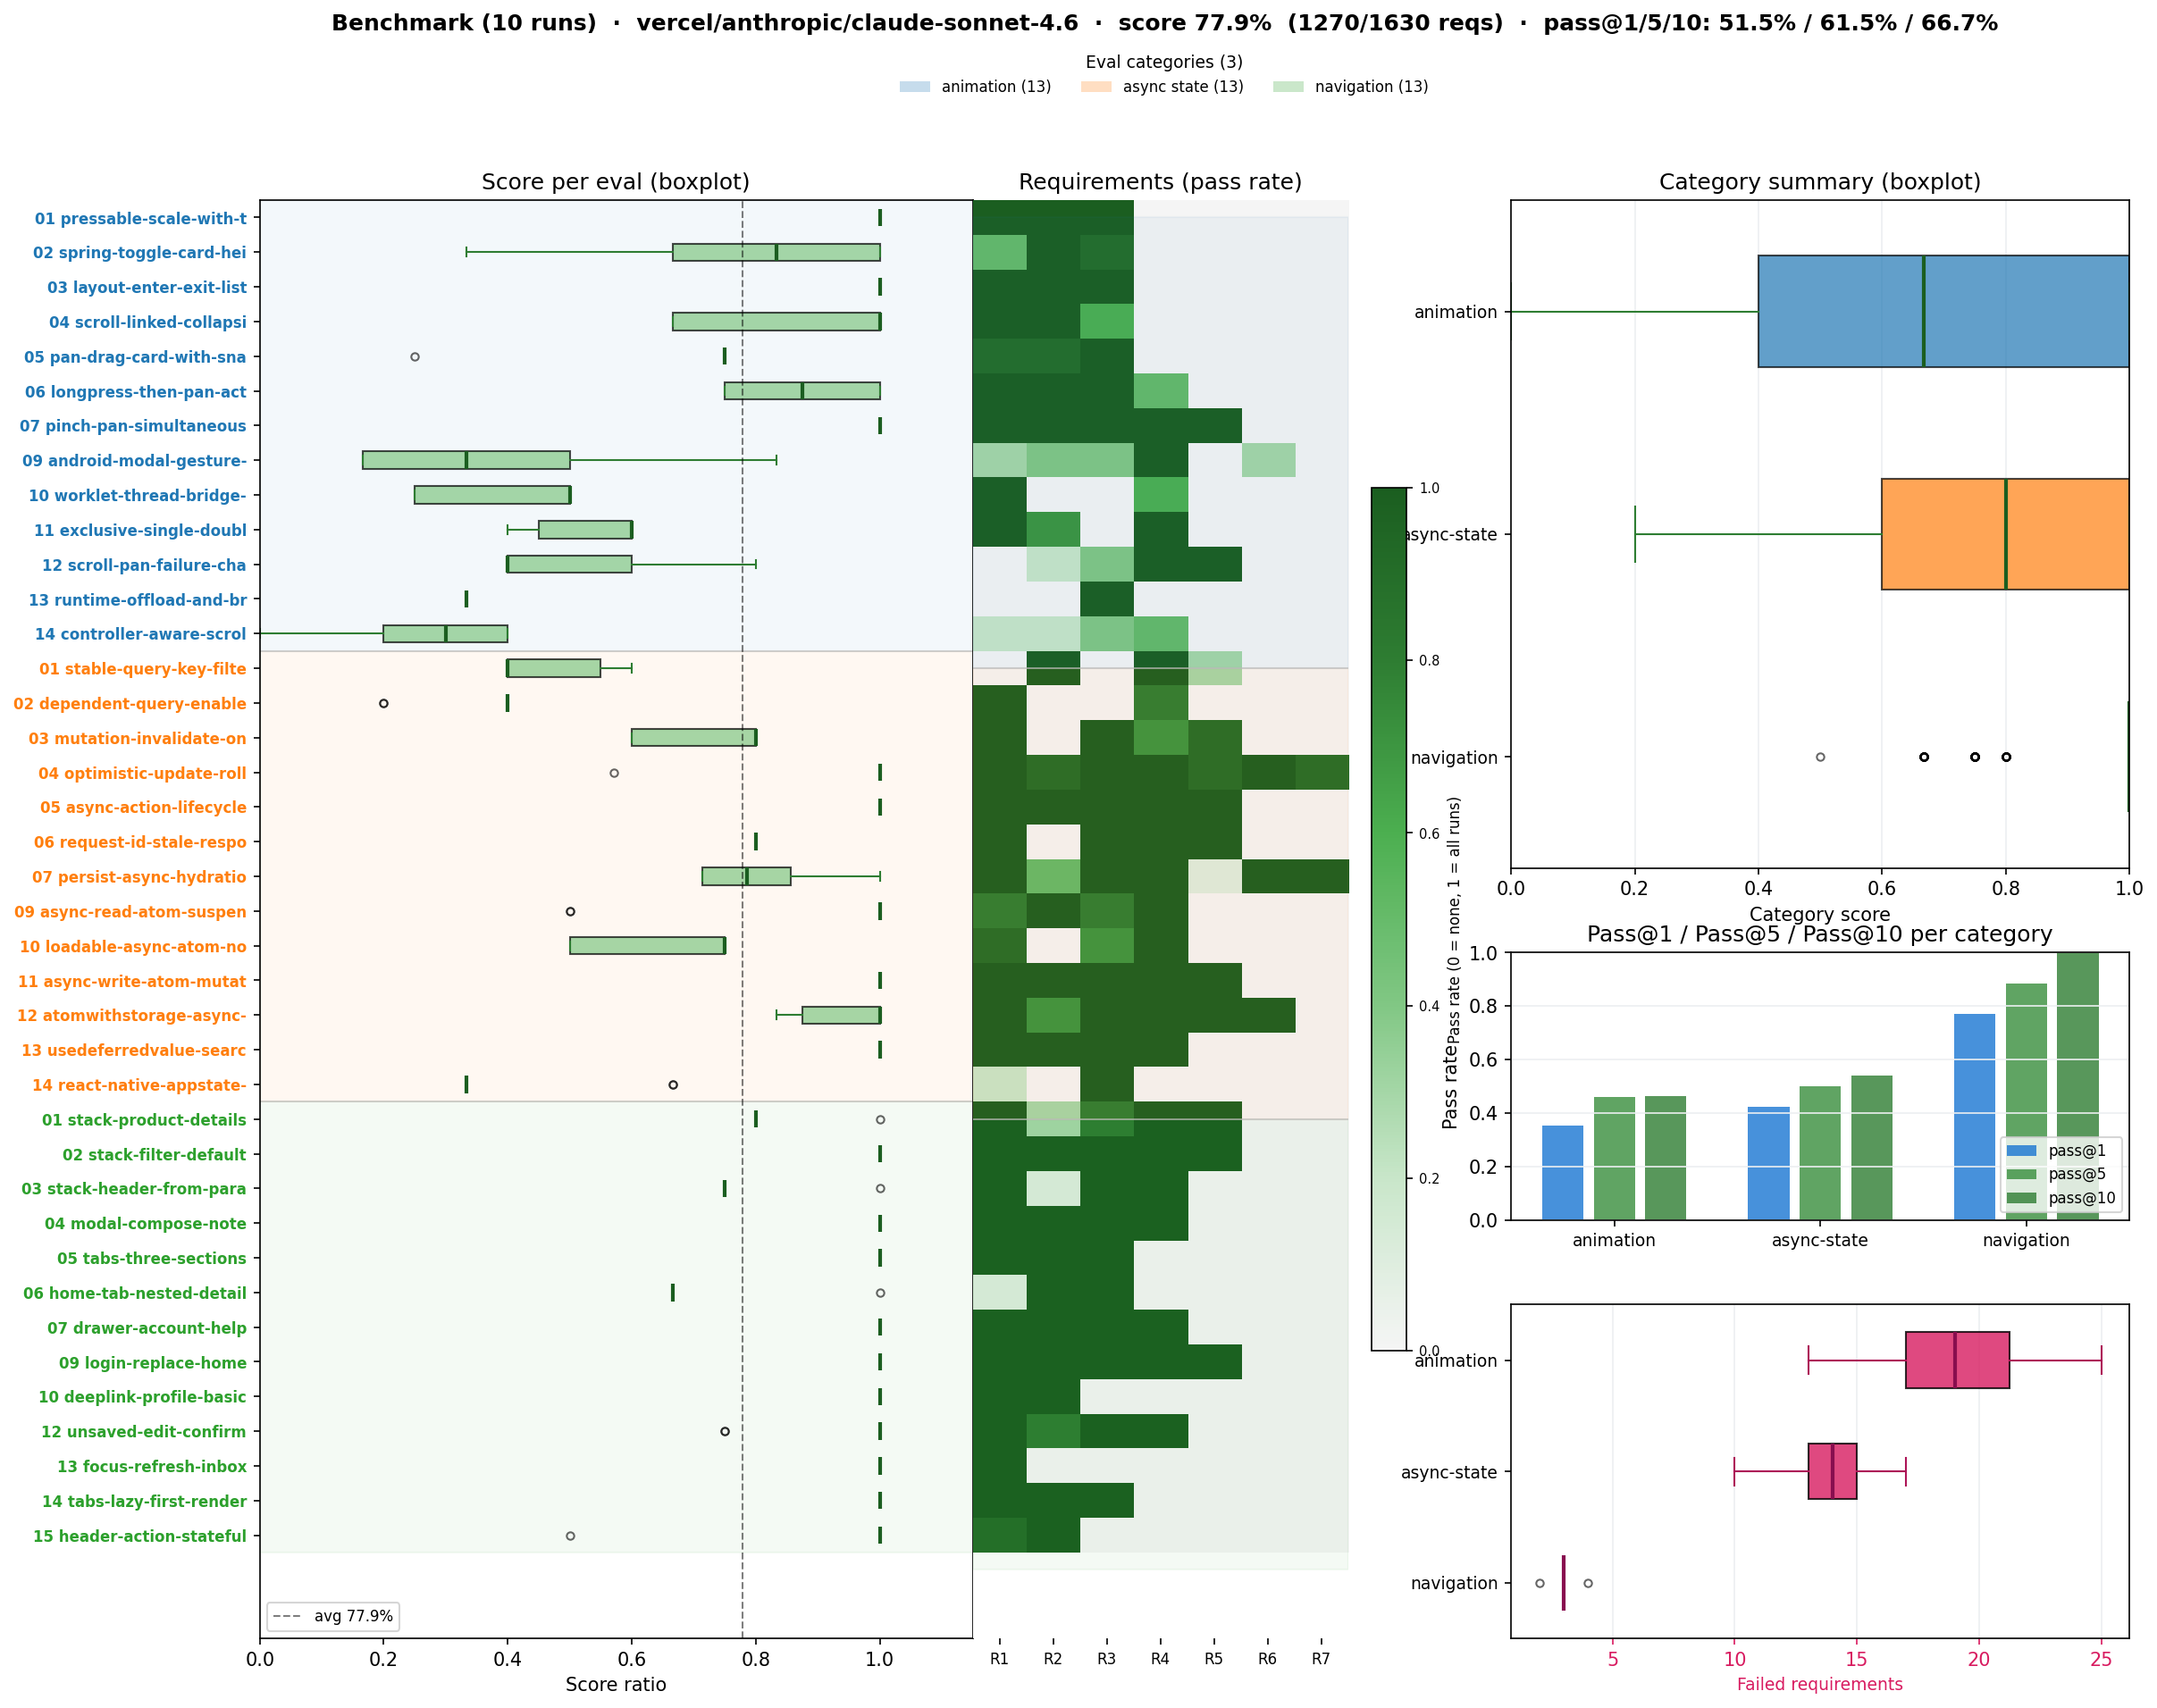
\includegraphics[width=\textwidth]{export/figures/claude-sonnet-4.6_benchmark_plot.png}
\caption{Benchmark Plot for claude-sonnet-4.6.}
\end{figure}

\begin{figure}[htbp]
\centering
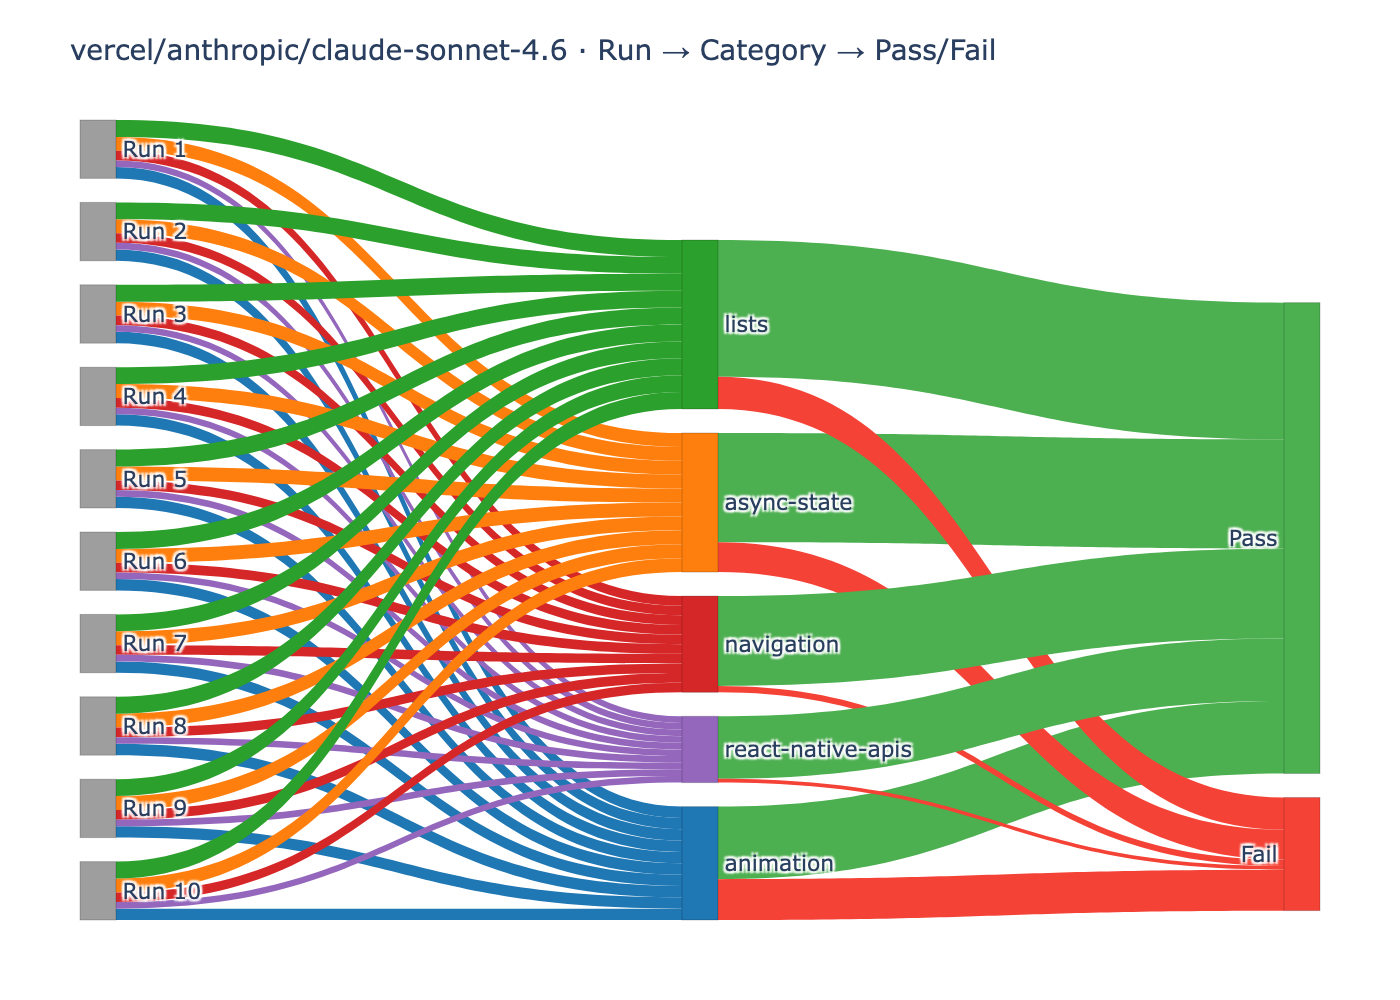
\includegraphics[width=\textwidth]{export/figures/claude-sonnet-4.6_sankey_per_run.png}
\caption{Sankey per run for claude-sonnet-4.6 showing the distribution of evals with respect to categories and results}
\end{figure}


\clearpage

\subsection{deepseek-r1-distill-qwen-32b}

% Table: summary
% Requires: \usepackage{booktabs}
\begin{table}[htbp]
\centering
\begin{tabular}{lrrrrrr}
\toprule
Model & Runs & Score & Reqs & P@1 & P@5 & P@10 \\
\midrule
cloudflare-ai-gateway/workers-ai/@cf/deepseek-ai/d & 10 & 44.4\% & 1211/2730 & 19.2\% & 31.1\% & 36.4\% \\
\bottomrule
\end{tabular}
\caption{Model summary for deepseek-r1-distill-qwen-32b}
\end{table}


% Table: category_summary
% Requires: \usepackage{booktabs}
\begin{table}[htbp]
\centering
\begin{tabular}{lrrrr}
\toprule
Category & Score & Evals & Requirements & Failed requirements \\
\midrule
animation & 11.1\% & 130 & 53 & 483 \\
async state & 32.7\% & 130 & 65 & 438 \\
lists & 55.7\% & 180 & 79 & 356 \\
navigation & 57.3\% & 130 & 45 & 190 \\
react native apis & 82.1\% & 90 & 31 & 52 \\
\bottomrule
\end{tabular}
\caption{Results by category for deepseek-r1-distill-qwen-32b. Score: mean(per-eval passed/total weight) across evals and runs. Evals: count of evaluation tasks. Requirements: sum of requirement count per eval. Failed requirements: sum of failed requirement instances across runs.}
\end{table}


% Table: per_eval
% Requires: \usepackage{booktabs}
\begin{table}[htbp]
\centering
\begin{adjustbox}{width=0.8\textwidth}
\begin{tabular}{lrrrrr}
\toprule
Eval & Category & Score & P@1 & P@5 & P@10 \\
\midrule
01-rn-anim-pressable-scale-with-timing & animation & 53.3\% & 10.0\% & 50.0\% & 100.0\% \\
02-rn-anim-spring-toggle-card-height & animation & 6.7\% & 0.0\% & 0.0\% & 0.0\% \\
03-rn-anim-layout-enter-exit-list-items & animation & 40.0\% & 10.0\% & 50.0\% & 100.0\% \\
04-rn-anim-scroll-linked-collapsing-header & animation & 6.7\% & 0.0\% & 0.0\% & 0.0\% \\
05-rn-anim-pan-drag-card-with-snap-points & animation & 2.5\% & 0.0\% & 0.0\% & 0.0\% \\
06-rn-anim-longpress-then-pan-activation-gate & animation & 7.5\% & 0.0\% & 0.0\% & 0.0\% \\
07-rn-anim-pinch-pan-simultaneous-photo-canvas & animation & 4.0\% & 0.0\% & 0.0\% & 0.0\% \\
09-rn-anim-android-modal-gesture-root-safety & animation & 5.0\% & 0.0\% & 0.0\% & 0.0\% \\
10-rn-anim-worklet-thread-bridge-schedule-on-rn & animation & 0.0\% & 0.0\% & 0.0\% & 0.0\% \\
11-rn-rngh-exclusive-single-double-tap & animation & 0.0\% & 0.0\% & 0.0\% & 0.0\% \\
12-rn-rngh-scroll-pan-failure-chain & animation & 0.0\% & 0.0\% & 0.0\% & 0.0\% \\
13-rn-worklets-runtime-offload-and-bridge & animation & 16.7\% & 0.0\% & 0.0\% & 0.0\% \\
14-rn-keyboard-controller-aware-scroll-footer & animation & 2.0\% & 0.0\% & 0.0\% & 0.0\% \\
01-rn-rq-stable-query-key-filters & async state & 6.0\% & 0.0\% & 0.0\% & 0.0\% \\
02-rn-rq-dependent-query-enabled-gate & async state & 18.0\% & 0.0\% & 0.0\% & 0.0\% \\
03-rn-rq-mutation-invalidate-on-success & async state & 2.0\% & 0.0\% & 0.0\% & 0.0\% \\
04-rn-rq-optimistic-update-rollback & async state & 11.4\% & 0.0\% & 0.0\% & 0.0\% \\
05-rn-zustand-async-action-lifecycle & async state & 86.0\% & 50.0\% & 99.6\% & 100.0\% \\
06-rn-zustand-request-id-stale-response-guard & async state & 40.0\% & 0.0\% & 0.0\% & 0.0\% \\
07-rn-zustand-persist-async-hydration-gate & async state & 28.6\% & 0.0\% & 0.0\% & 0.0\% \\
09-rn-jotai-async-read-atom-suspense & async state & 57.5\% & 20.0\% & 77.8\% & 100.0\% \\
10-rn-jotai-loadable-async-atom-no-suspense & async state & 0.0\% & 0.0\% & 0.0\% & 0.0\% \\
11-rn-jotai-async-write-atom-mutation & async state & 38.0\% & 0.0\% & 0.0\% & 0.0\% \\
12-rn-jotai-atomwithstorage-async-rehydrate-guard & async state & 68.3\% & 0.0\% & 0.0\% & 0.0\% \\
13-rn-react-usedeferredvalue-search-stale-indicator & async state & 42.5\% & 10.0\% & 50.0\% & 100.0\% \\
14-rn-rq-react-native-appstate-focus-online-managers & async state & 26.7\% & 0.0\% & 0.0\% & 0.0\% \\
01-rn-flatlist-scroll-to-unread-fixed-rows & lists & 44.0\% & 0.0\% & 0.0\% & 0.0\% \\
02-rn-flatlist-basic-contact-list & lists & 100.0\% & 100.0\% & 100.0\% & 100.0\% \\
03-rn-flatlist-two-column-product-grid & lists & 93.3\% & 80.0\% & 100.0\% & 100.0\% \\
04-rn-flatlist-viewability-impression-tracking & lists & 66.0\% & 0.0\% & 0.0\% & 0.0\% \\
05-rn-flatlist-large-feed-window-tuning & lists & 60.0\% & 0.0\% & 0.0\% & 0.0\% \\
06-rn-flatlist-pull-to-refresh-feed & lists & 80.0\% & 0.0\% & 0.0\% & 0.0\% \\
07-rn-flatlist-to-sectionlist-conversion & lists & 88.0\% & 40.0\% & 97.6\% & 100.0\% \\
08-rn-flashlist-basic-list & lists & 76.7\% & 50.0\% & 99.6\% & 100.0\% \\
09-rn-flashlist-horizontal-rail-list-header & lists & 42.5\% & 0.0\% & 0.0\% & 0.0\% \\
10-rn-flashlist-horizontal-dynamic-height-header-first-item & lists & 53.3\% & 0.0\% & 0.0\% & 0.0\% \\
11-rn-flashlist-expandable-cards-layout-state & lists & 36.7\% & 0.0\% & 0.0\% & 0.0\% \\
12-rn-flashlist-chat-start-from-bottom & lists & 34.0\% & 0.0\% & 0.0\% & 0.0\% \\
13-rn-flashlist-masonry-photo-gallery & lists & 52.0\% & 0.0\% & 0.0\% & 0.0\% \\
14-rn-flatlist-to-legendlist-migration & lists & 20.0\% & 0.0\% & 0.0\% & 0.0\% \\
15-rn-legendlist-sticky-grouped-agenda & lists & 48.0\% & 0.0\% & 0.0\% & 0.0\% \\
16-rn-legendlist-section-scroll-to-location & lists & 52.0\% & 10.0\% & 50.0\% & 100.0\% \\
17-rn-legendlist-chat-start-from-bottom & lists & 28.0\% & 0.0\% & 0.0\% & 0.0\% \\
18-rn-legendlist-expandable-cards-recycling-state & lists & 27.5\% & 0.0\% & 0.0\% & 0.0\% \\
01-rn-nav-stack-product-details & navigation & 60.0\% & 0.0\% & 0.0\% & 0.0\% \\
02-rn-nav-stack-filter-default & navigation & 98.0\% & 90.0\% & 100.0\% & 100.0\% \\
03-rn-nav-stack-header-from-param & navigation & 50.0\% & 0.0\% & 0.0\% & 0.0\% \\
04-rn-nav-modal-compose-note & navigation & 82.5\% & 40.0\% & 97.6\% & 100.0\% \\
05-rn-nav-tabs-three-sections & navigation & 60.0\% & 30.0\% & 91.7\% & 100.0\% \\
06-rn-nav-home-tab-nested-details & navigation & 70.0\% & 30.0\% & 91.7\% & 100.0\% \\
07-rn-nav-drawer-account-help & navigation & 45.0\% & 10.0\% & 50.0\% & 100.0\% \\
09-rn-nav-login-replace-home & navigation & 22.0\% & 0.0\% & 0.0\% & 0.0\% \\
10-rn-nav-deeplink-profile-basic & navigation & 25.0\% & 10.0\% & 50.0\% & 100.0\% \\
12-rn-nav-unsaved-edit-confirm & navigation & 52.5\% & 0.0\% & 0.0\% & 0.0\% \\
13-rn-nav-focus-refresh-inbox & navigation & 100.0\% & 100.0\% & 100.0\% & 100.0\% \\
14-rn-nav-tabs-lazy-first-render & navigation & 80.0\% & 40.0\% & 97.6\% & 100.0\% \\
15-rn-nav-header-action-stateful & navigation & 0.0\% & 0.0\% & 0.0\% & 0.0\% \\
01-rn-stylesheet-card-variants & react native apis & 76.7\% & 50.0\% & 99.6\% & 100.0\% \\
02-rn-stylesheet-absolute-fill-overlay-badge & react native apis & 66.7\% & 0.0\% & 0.0\% & 0.0\% \\
03-rn-stylesheet-divider-hairline & react native apis & 43.3\% & 0.0\% & 0.0\% & 0.0\% \\
04-rn-image-network-dimensions & react native apis & 100.0\% & 100.0\% & 100.0\% & 100.0\% \\
05-rn-imagebackground-resize-mode & react native apis & 62.5\% & 0.0\% & 0.0\% & 0.0\% \\
06-rn-platform-select-small-style-delta & react native apis & 100.0\% & 100.0\% & 100.0\% & 100.0\% \\
07-rn-platform-os-conditional-cta & react native apis & 100.0\% & 100.0\% & 100.0\% & 100.0\% \\
08-rn-platform-file-extension-component-split & react native apis & 100.0\% & 100.0\% & 100.0\% & 100.0\% \\
09-rn-keyboardavoidingview-login-form & react native apis & 90.0\% & 90.0\% & 100.0\% & 100.0\% \\
\bottomrule
\end{tabular}
\end{adjustbox}
\caption{Per-eval results (score and pass@k) for deepseek-r1-distill-qwen-32b}
\end{table}


\begin{figure}[htbp]
\centering
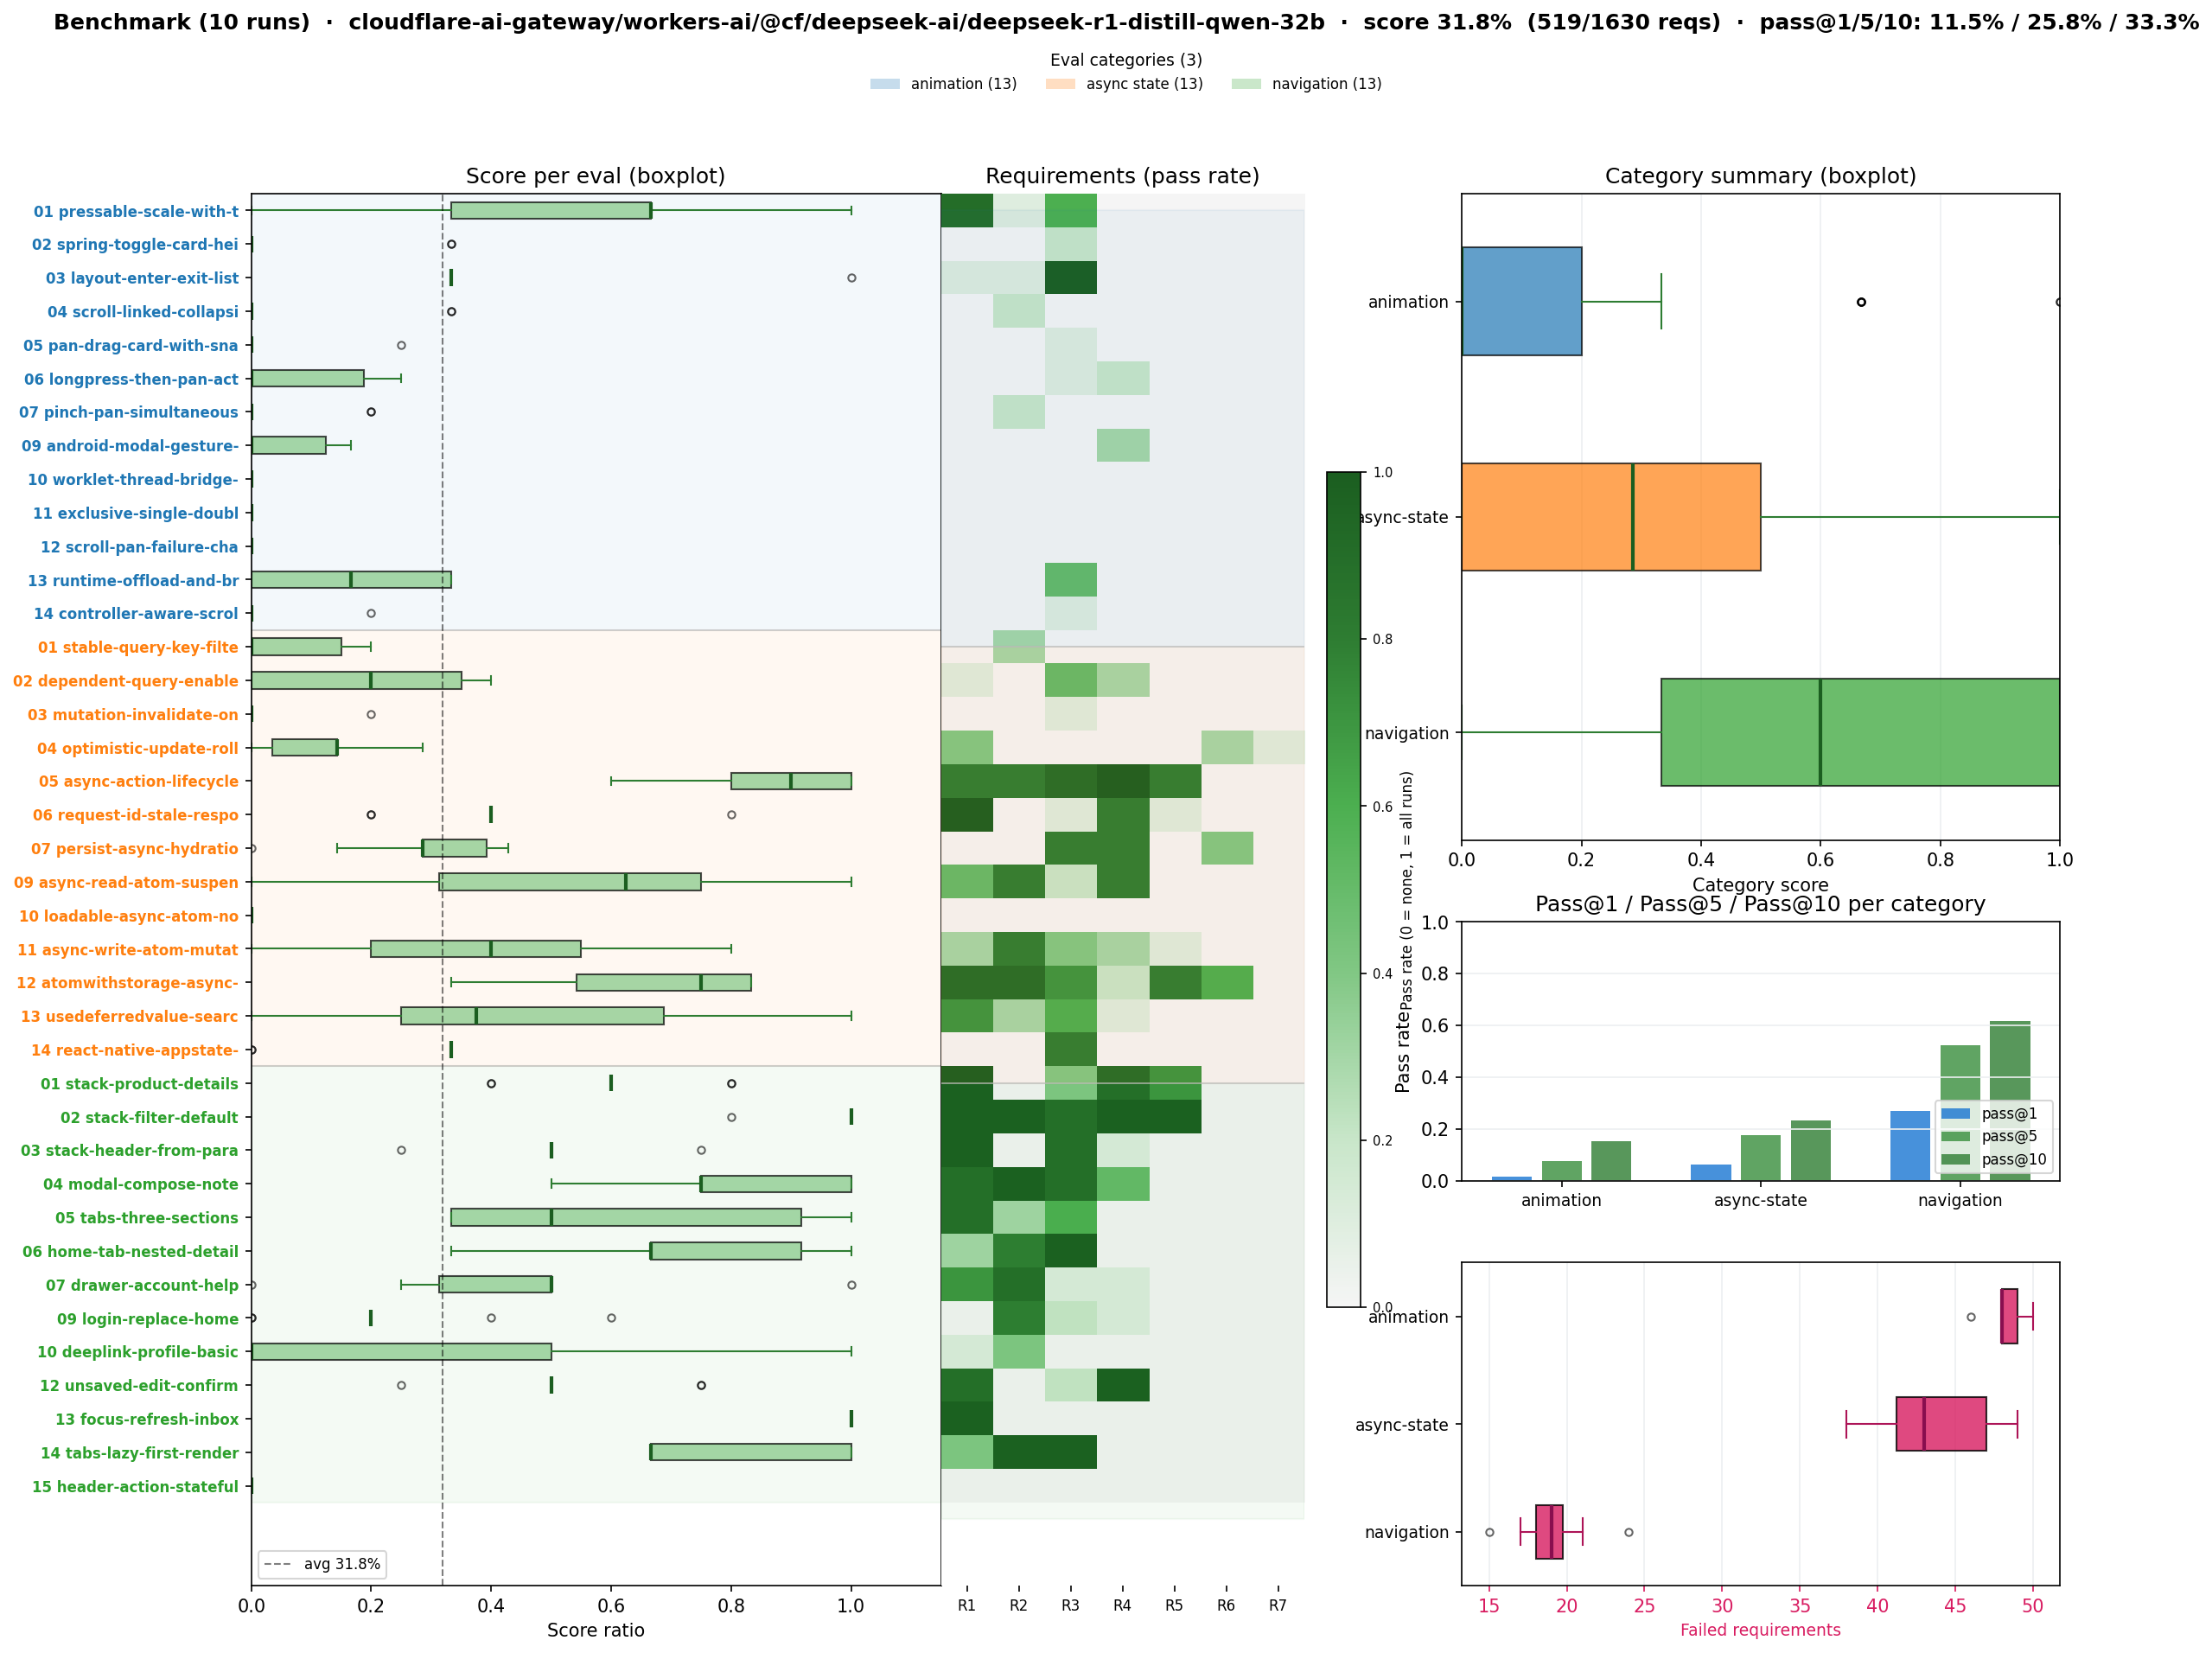
\includegraphics[width=\textwidth]{export/figures/deepseek-r1-distill-qwen-32b_benchmark_plot.png}
\caption{Benchmark Plot for deepseek-r1-distill-qwen-32b.}
\end{figure}

\begin{figure}[htbp]
\centering
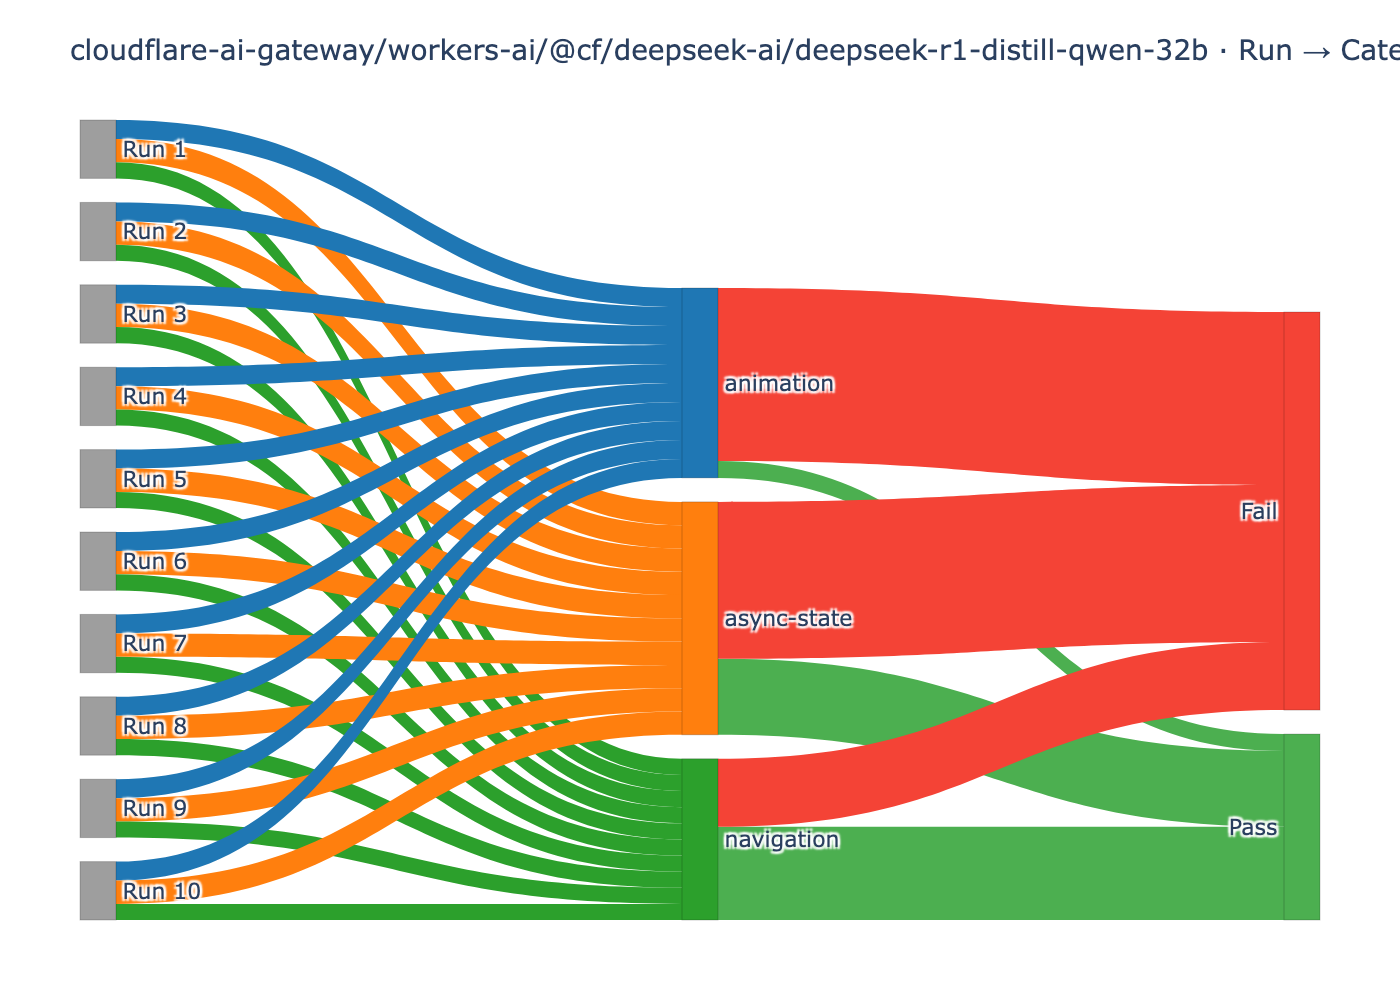
\includegraphics[width=\textwidth]{export/figures/deepseek-r1-distill-qwen-32b_sankey_per_run.png}
\caption{Sankey per run for deepseek-r1-distill-qwen-32b showing the distribution of evals with respect to categories and results}
\end{figure}


\clearpage

\subsection{deepseek-v3.2}

% Table: summary
% Requires: \usepackage{booktabs}
\begin{table}[htbp]
\centering
\begin{tabular}{lrrrrrr}
\toprule
Model & Runs & Score & Reqs & P@1 & P@5 & P@10 \\
\midrule
vercel/deepseek/deepseek-v3.2 & 10 & 69.0\% & 1118/1621 & 41.0\% & 56.8\% & 59.0\% \\
\bottomrule
\end{tabular}
\caption{Model summary for deepseek-v3.2}
\end{table}


% Table: category_summary
% Requires: \usepackage{booktabs}
\begin{table}[htbp]
\centering
\begin{tabular}{lrrrr}
\toprule
Category & Score & Evals & Requirements & Failed requirements \\
\midrule
animation & 57.5\% & 129 & 53 & 233 \\
async state & 71.0\% & 130 & 65 & 182 \\
lists & 68.5\% & 180 & 79 & 245 \\
navigation & 80.4\% & 129 & 45 & 88 \\
react native apis & 89.9\% & 90 & 31 & 28 \\
\bottomrule
\end{tabular}
\caption{Results by category for deepseek-v3.2. Score: mean(per-eval passed/total weight) across evals and runs. Evals: count of evaluation tasks. Requirements: sum of requirement count per eval. Failed requirements: sum of failed requirement instances across runs.}
\end{table}


% Table: per_eval
% Requires: \usepackage{booktabs}
\begin{table}[htbp]
\centering
\begin{tabular}{lrrrrr}
\toprule
Eval & Category & Score & P@1 & P@5 & P@10 \\
\midrule
01-rn-anim-pressable-scale-with-timing & animation & 70.0\% & 30.0\% & 91.7\% & 100.0\% \\
02-rn-anim-spring-toggle-card-height & animation & 66.7\% & 30.0\% & 91.7\% & 100.0\% \\
03-rn-anim-layout-enter-exit-list-items & animation & 86.7\% & 80.0\% & 100.0\% & 100.0\% \\
04-rn-anim-scroll-linked-collapsing-header & animation & 93.3\% & 90.0\% & 100.0\% & 100.0\% \\
05-rn-anim-pan-drag-card-with-snap-points & animation & 52.5\% & 0.0\% & 0.0\% & 0.0\% \\
06-rn-anim-longpress-then-pan-activation-gate & animation & 82.5\% & 50.0\% & 99.6\% & 100.0\% \\
07-rn-anim-pinch-pan-simultaneous-photo-canvas & animation & 98.0\% & 90.0\% & 100.0\% & 100.0\% \\
09-rn-anim-android-modal-gesture-root-safety & animation & 48.3\% & 0.0\% & 0.0\% & 0.0\% \\
10-rn-anim-worklet-thread-bridge-schedule-on-rn & animation & 22.2\% & 0.0\% & 0.0\% & 0.0\% \\
11-rn-rngh-exclusive-single-double-tap & animation & 30.0\% & 0.0\% & 0.0\% & 0.0\% \\
12-rn-rngh-scroll-pan-failure-chain & animation & 60.0\% & 0.0\% & 0.0\% & 0.0\% \\
13-rn-worklets-runtime-offload-and-bridge & animation & 20.0\% & 0.0\% & 0.0\% & 0.0\% \\
14-rn-keyboard-controller-aware-scroll-footer & animation & 14.0\% & 0.0\% & 0.0\% & 0.0\% \\
01-rn-rq-stable-query-key-filters & async state & 34.0\% & 0.0\% & 0.0\% & 0.0\% \\
02-rn-rq-dependent-query-enabled-gate & async state & 34.0\% & 0.0\% & 0.0\% & 0.0\% \\
03-rn-rq-mutation-invalidate-on-success & async state & 72.0\% & 0.0\% & 0.0\% & 0.0\% \\
04-rn-rq-optimistic-update-rollback & async state & 91.4\% & 60.0\% & 100.0\% & 100.0\% \\
05-rn-zustand-async-action-lifecycle & async state & 100.0\% & 100.0\% & 100.0\% & 100.0\% \\
06-rn-zustand-request-id-stale-response-guard & async state & 78.0\% & 30.0\% & 91.7\% & 100.0\% \\
07-rn-zustand-persist-async-hydration-gate & async state & 60.0\% & 0.0\% & 0.0\% & 0.0\% \\
09-rn-jotai-async-read-atom-suspense & async state & 92.5\% & 70.0\% & 100.0\% & 100.0\% \\
10-rn-jotai-loadable-async-atom-no-suspense & async state & 22.5\% & 0.0\% & 0.0\% & 0.0\% \\
11-rn-jotai-async-write-atom-mutation & async state & 94.0\% & 80.0\% & 100.0\% & 100.0\% \\
12-rn-jotai-atomwithstorage-async-rehydrate-guard & async state & 91.7\% & 50.0\% & 99.6\% & 100.0\% \\
13-rn-react-usedeferredvalue-search-stale-indicator & async state & 92.5\% & 70.0\% & 100.0\% & 100.0\% \\
14-rn-rq-react-native-appstate-focus-online-managers & async state & 60.0\% & 30.0\% & 91.7\% & 100.0\% \\
01-rn-nav-stack-product-details & navigation & 68.0\% & 0.0\% & 0.0\% & 0.0\% \\
02-rn-nav-stack-filter-default & navigation & 100.0\% & 100.0\% & 100.0\% & 100.0\% \\
03-rn-nav-stack-header-from-param & navigation & 55.0\% & 10.0\% & 50.0\% & 100.0\% \\
04-rn-nav-modal-compose-note & navigation & 100.0\% & 100.0\% & 100.0\% & 100.0\% \\
05-rn-nav-tabs-three-sections & navigation & 96.7\% & 90.0\% & 100.0\% & 100.0\% \\
06-rn-nav-home-tab-nested-details & navigation & 90.0\% & 70.0\% & 100.0\% & 100.0\% \\
07-rn-nav-drawer-account-help & navigation & 100.0\% & 100.0\% & 100.0\% & 100.0\% \\
09-rn-nav-login-replace-home & navigation & 57.8\% & 0.0\% & 0.0\% & 0.0\% \\
10-rn-nav-deeplink-profile-basic & navigation & 100.0\% & 100.0\% & 100.0\% & 100.0\% \\
12-rn-nav-unsaved-edit-confirm & navigation & 75.0\% & 0.0\% & 0.0\% & 0.0\% \\
13-rn-nav-focus-refresh-inbox & navigation & 100.0\% & 100.0\% & 100.0\% & 100.0\% \\
14-rn-nav-tabs-lazy-first-render & navigation & 90.0\% & 70.0\% & 100.0\% & 100.0\% \\
15-rn-nav-header-action-stateful & navigation & 10.0\% & 0.0\% & 0.0\% & 0.0\% \\
\bottomrule
\end{tabular}
\caption{Per-eval results (score and pass@k) for deepseek-v3.2}
\end{table}


\begin{figure}[htbp]
\centering
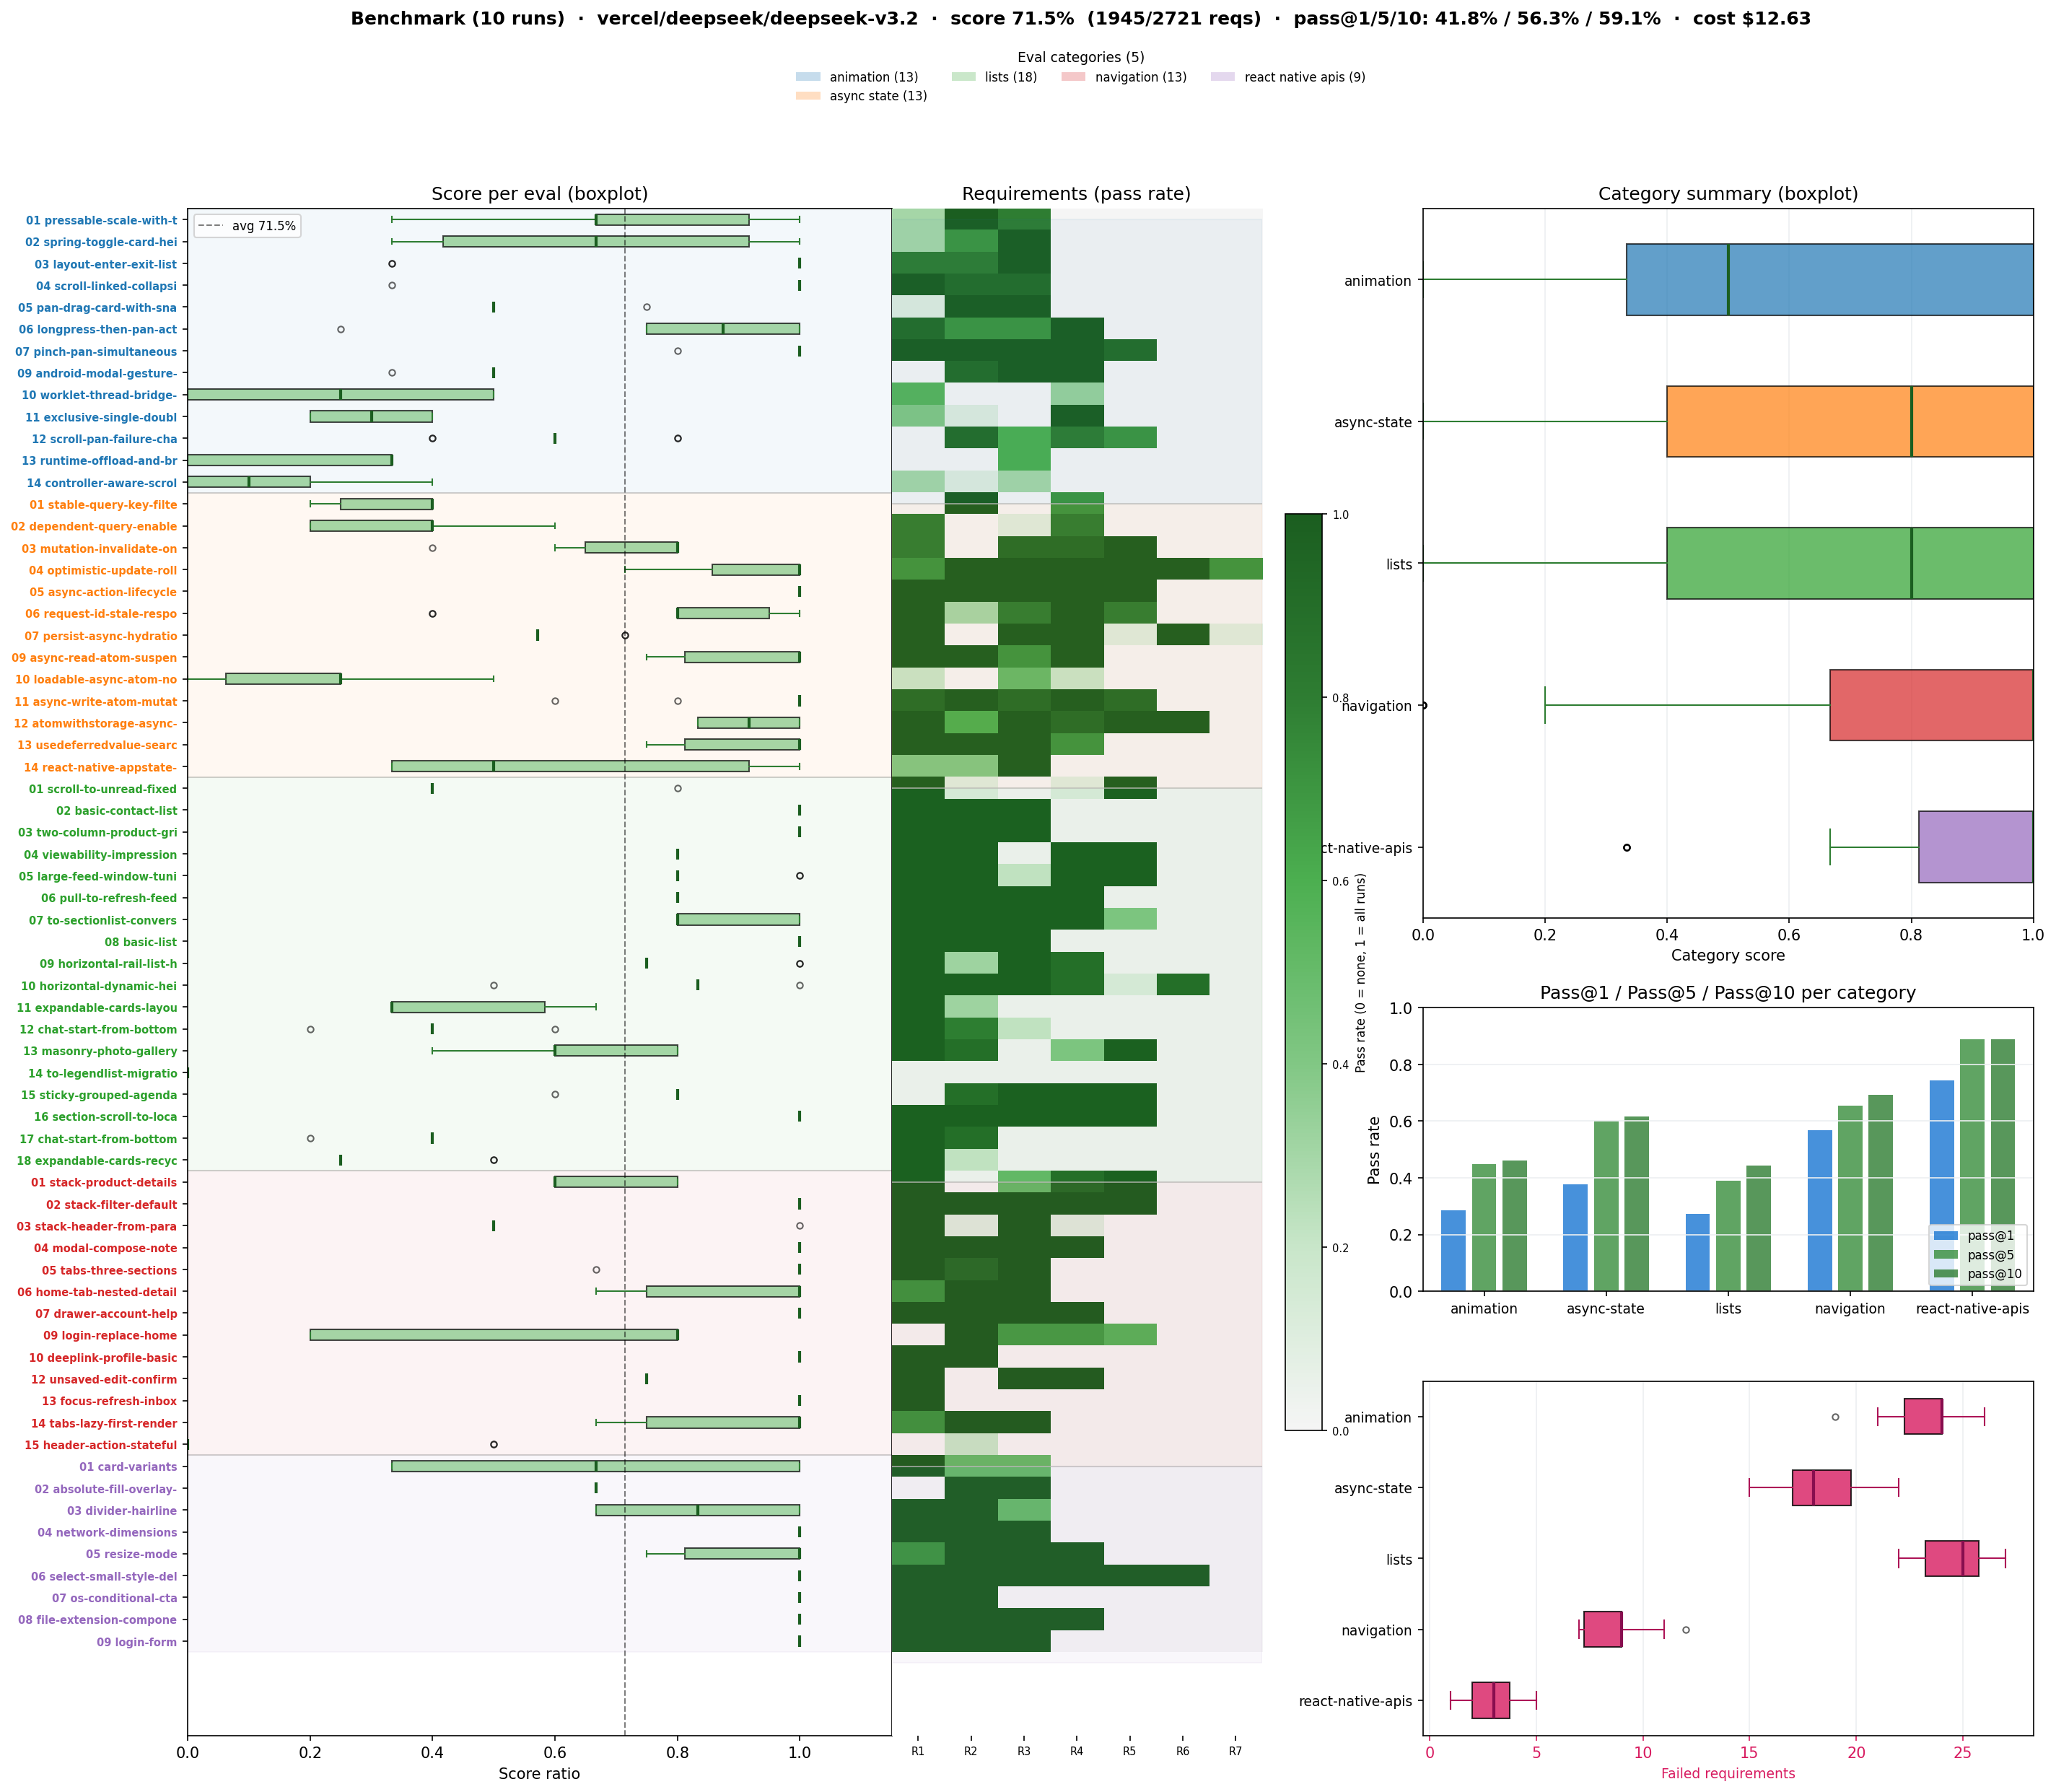
\includegraphics[width=\textwidth]{export/figures/deepseek-v3.2_benchmark_plot.png}
\caption{Benchmark Plot for deepseek-v3.2.}
\end{figure}

\begin{figure}[htbp]
\centering
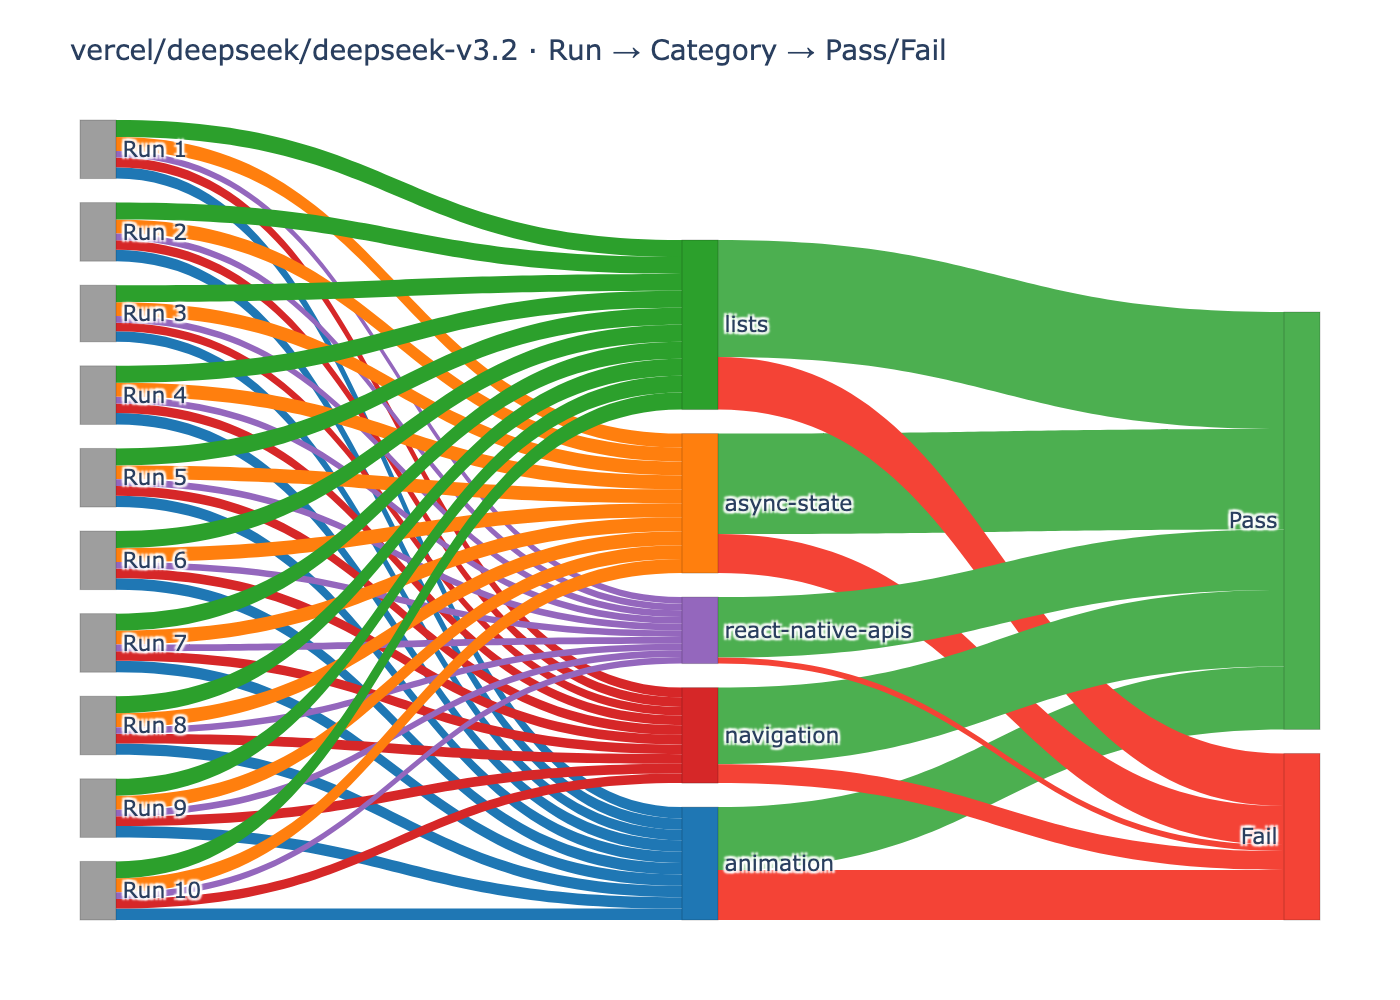
\includegraphics[width=\textwidth]{export/figures/deepseek-v3.2_sankey_per_run.png}
\caption{Sankey per run for deepseek-v3.2 showing the distribution of evals with respect to categories and results}
\end{figure}


\clearpage

\subsection{gemini-3.1-pro-preview}

% Table: summary
% Requires: \usepackage{booktabs}
\begin{table}[htbp]
\centering
\begin{tabular}{lrrrrrr}
\toprule
Model & Runs & Score & Reqs & P@1 & P@5 & P@10 \\
\midrule
vercel/google/gemini-3.1-pro-preview & 10 & 78.9\% & 1286/1630 & 52.3\% & 60.2\% & 64.1\% \\
\bottomrule
\end{tabular}
\caption{Model summary for gemini-3.1-pro-preview}
\end{table}


% Table: category_summary
% Requires: \usepackage{booktabs}
\begin{table}[htbp]
\centering
\begin{tabular}{lrrrr}
\toprule
Category & Score & Evals & Requirements & Failed requirements \\
\midrule
animation & 65.1\% & 130 & 53 & 189 \\
async state & 78.9\% & 130 & 65 & 130 \\
lists & 73.7\% & 180 & 79 & 215 \\
navigation & 95.0\% & 130 & 45 & 25 \\
react native apis & 93.7\% & 90 & 31 & 17 \\
\bottomrule
\end{tabular}
\caption{Results by category for gemini-3.1-pro-preview. Score: mean(per-eval passed/total weight) across evals and runs. Evals: count of evaluation tasks. Requirements: sum of requirement count per eval. Failed requirements: sum of failed requirement instances across runs.}
\end{table}


% Table: per_eval
\input{export/tables/gemini-3.1-pro-preview_per_eval}

\begin{figure}[htbp]
\centering
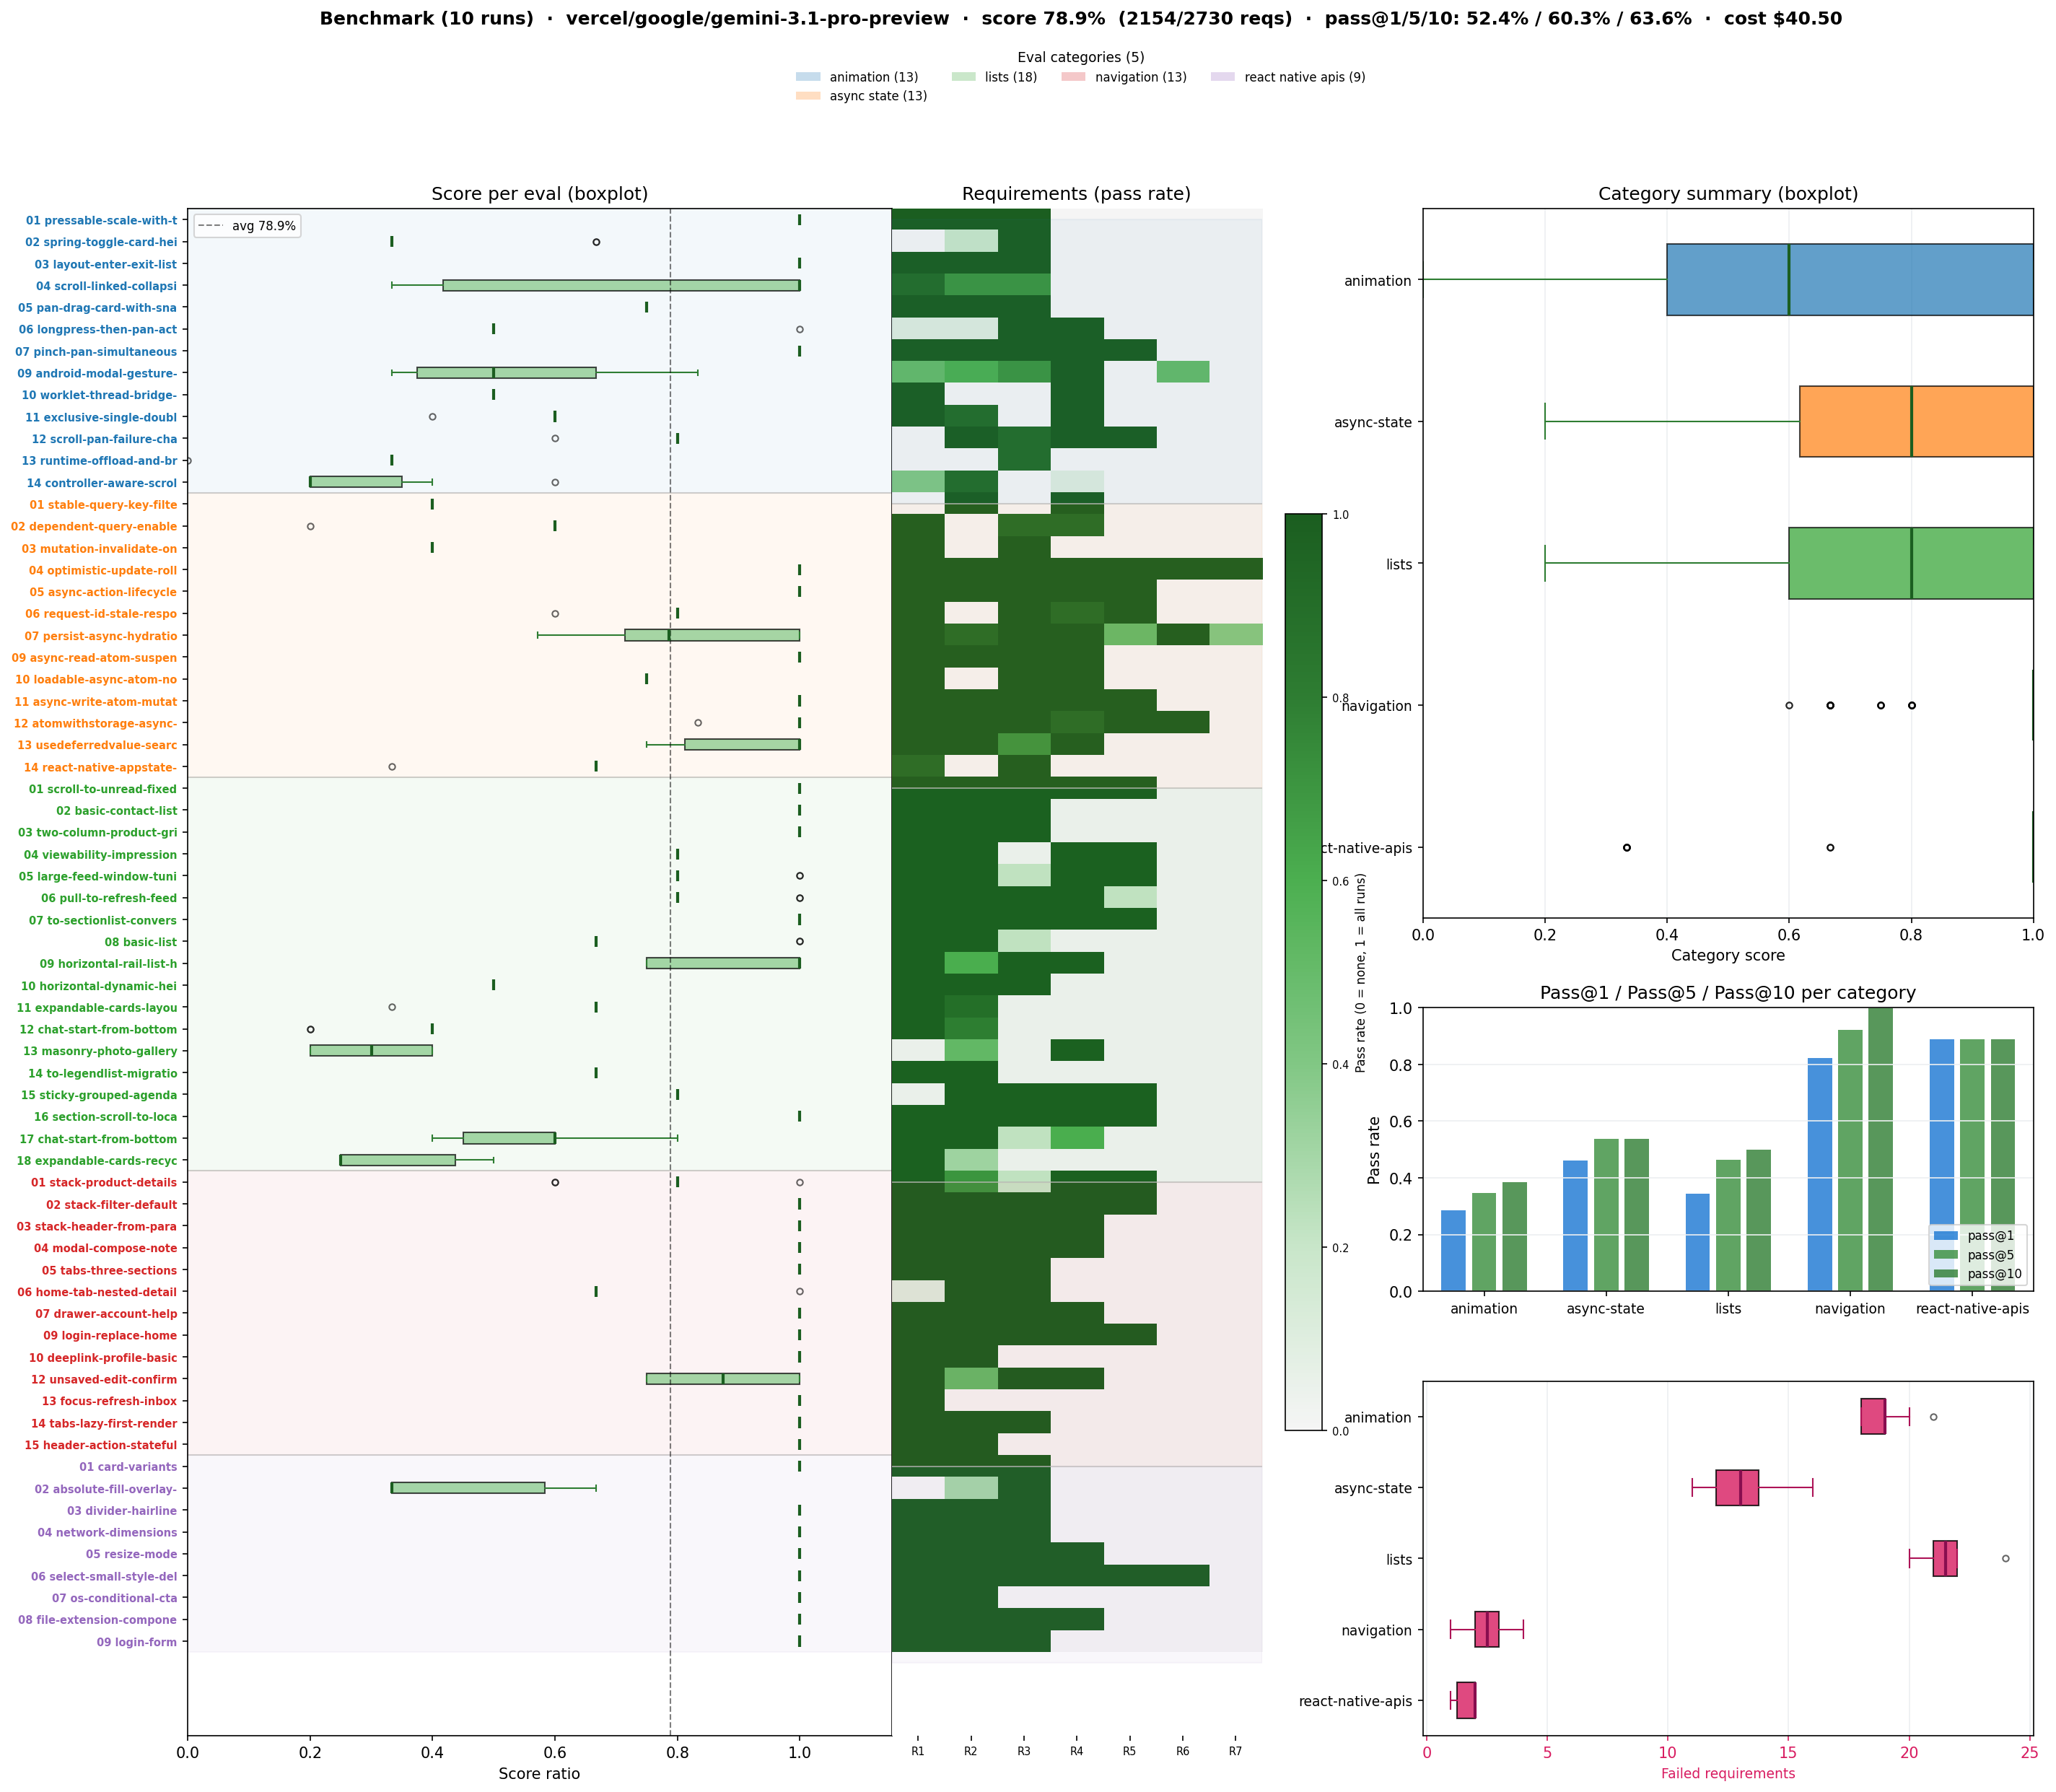
\includegraphics[width=\textwidth]{export/figures/gemini-3.1-pro-preview_benchmark_plot.png}
\caption{Benchmark Plot for gemini-3.1-pro-preview.}
\end{figure}

\begin{figure}[htbp]
\centering
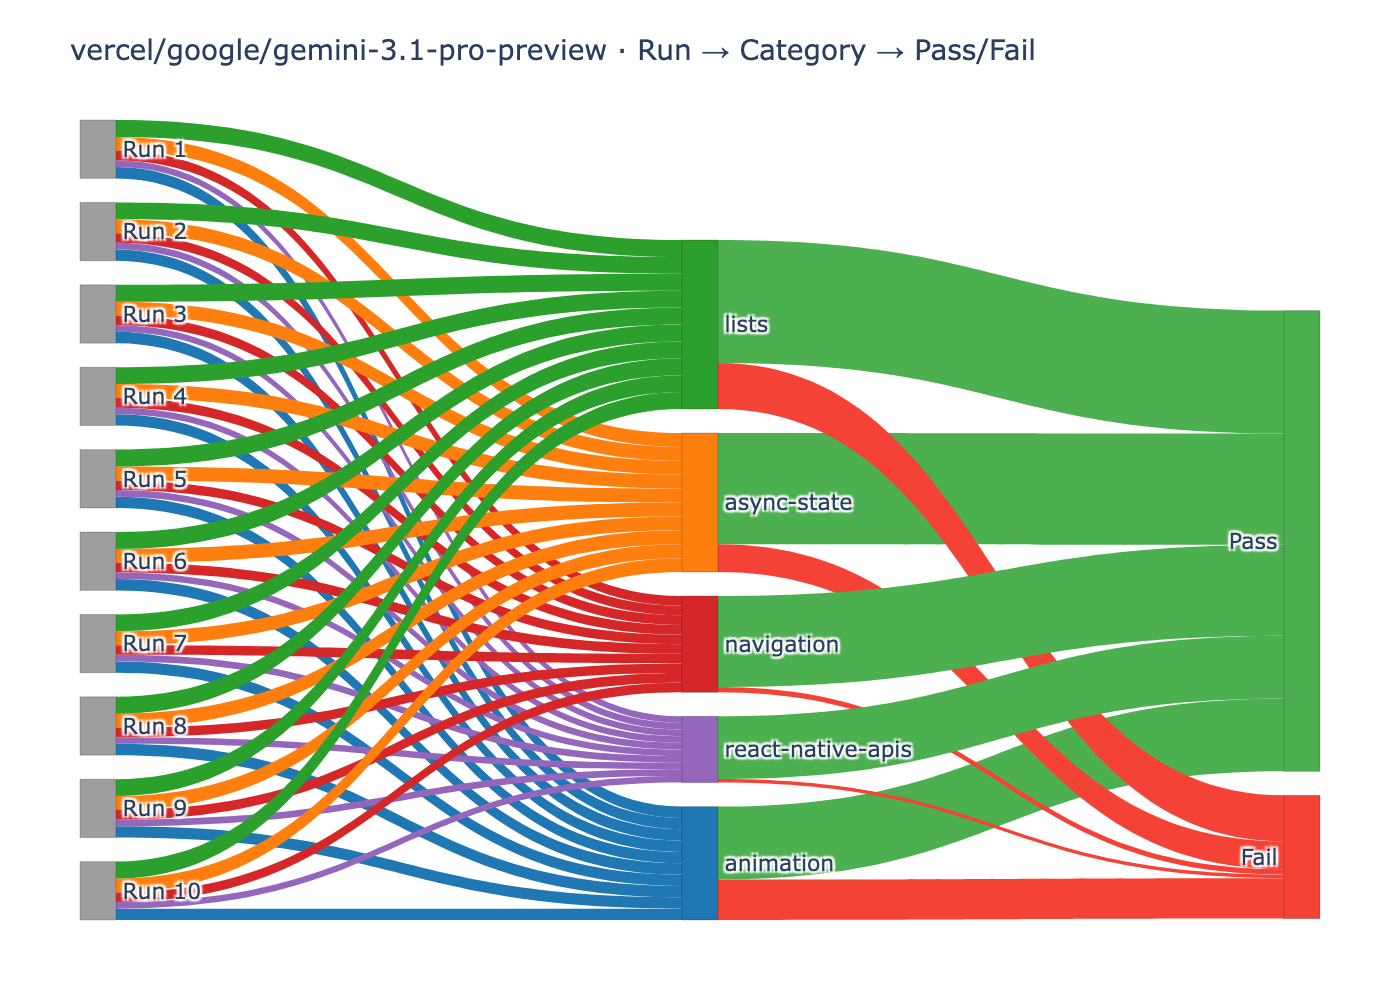
\includegraphics[width=\textwidth]{export/figures/gemini-3.1-pro-preview_sankey_per_run.png}
\caption{Sankey per run for gemini-3.1-pro-preview showing the distribution of evals with respect to categories and results}
\end{figure}


\clearpage

\subsection{glm-5}

% Table: summary
% Requires: \usepackage{booktabs}
\begin{table}[htbp]
\centering
\begin{tabular}{lrrrrrr}
\toprule
Model & Runs & Score & Reqs & P@1 & P@5 & P@10 \\
\midrule
vercel/zai/glm-5 & 10 & 74.2\% & 1210/1630 & 50.8\% & 61.2\% & 61.5\% \\
\bottomrule
\end{tabular}
\caption{Model summary for glm-5}
\end{table}


% Table: category_summary
% Requires: \usepackage{booktabs}
\begin{table}[htbp]
\centering
\begin{tabular}{lrrrr}
\toprule
Category & Score & Evals & Requirements & Failed requirements \\
\midrule
animation & 66.1\% & 130 & 53 & 194 \\
async state & 72.1\% & 130 & 65 & 169 \\
navigation & 89.2\% & 130 & 45 & 57 \\
\bottomrule
\end{tabular}
\caption{Results by category for glm-5. Score: mean(per-eval passed/total weight) across evals and runs. Evals: count of evaluation tasks. Requirements: sum of requirement count per eval. Failed requirements: sum of failed requirement instances across runs.}
\end{table}


% Table: per_eval
% Requires: \usepackage{booktabs}
\begin{table}[htbp]
\centering
\begin{tabular}{lrrrrr}
\toprule
Eval & Category & Score & P@1 & P@5 & P@10 \\
\midrule
01-rn-anim-pressable-scale-with-timing & animation & 100.0\% & 100.0\% & 100.0\% & 100.0\% \\
02-rn-anim-spring-toggle-card-height & animation & 83.3\% & 50.0\% & 99.6\% & 100.0\% \\
03-rn-anim-layout-enter-exit-list-items & animation & 100.0\% & 100.0\% & 100.0\% & 100.0\% \\
04-rn-anim-scroll-linked-collapsing-header & animation & 86.7\% & 70.0\% & 100.0\% & 100.0\% \\
05-rn-anim-pan-drag-card-with-snap-points & animation & 52.5\% & 0.0\% & 0.0\% & 0.0\% \\
06-rn-anim-longpress-then-pan-activation-gate & animation & 82.5\% & 50.0\% & 99.6\% & 100.0\% \\
07-rn-anim-pinch-pan-simultaneous-photo-canvas & animation & 98.0\% & 90.0\% & 100.0\% & 100.0\% \\
09-rn-anim-android-modal-gesture-root-safety & animation & 46.7\% & 0.0\% & 0.0\% & 0.0\% \\
10-rn-anim-worklet-thread-bridge-schedule-on-rn & animation & 50.0\% & 0.0\% & 0.0\% & 0.0\% \\
11-rn-rngh-exclusive-single-double-tap & animation & 40.0\% & 0.0\% & 0.0\% & 0.0\% \\
12-rn-rngh-scroll-pan-failure-chain & animation & 74.0\% & 0.0\% & 0.0\% & 0.0\% \\
13-rn-worklets-runtime-offload-and-bridge & animation & 30.0\% & 0.0\% & 0.0\% & 0.0\% \\
14-rn-keyboard-controller-aware-scroll-footer & animation & 16.0\% & 0.0\% & 0.0\% & 0.0\% \\
01-rn-rq-stable-query-key-filters & async state & 40.0\% & 0.0\% & 0.0\% & 0.0\% \\
02-rn-rq-dependent-query-enabled-gate & async state & 42.0\% & 0.0\% & 0.0\% & 0.0\% \\
03-rn-rq-mutation-invalidate-on-success & async state & 58.0\% & 0.0\% & 0.0\% & 0.0\% \\
04-rn-rq-optimistic-update-rollback & async state & 98.6\% & 90.0\% & 100.0\% & 100.0\% \\
05-rn-zustand-async-action-lifecycle & async state & 100.0\% & 100.0\% & 100.0\% & 100.0\% \\
06-rn-zustand-request-id-stale-response-guard & async state & 68.0\% & 30.0\% & 91.7\% & 100.0\% \\
07-rn-zustand-persist-async-hydration-gate & async state & 64.3\% & 0.0\% & 0.0\% & 0.0\% \\
09-rn-jotai-async-read-atom-suspense & async state & 100.0\% & 100.0\% & 100.0\% & 100.0\% \\
10-rn-jotai-loadable-async-atom-no-suspense & async state & 40.0\% & 0.0\% & 0.0\% & 0.0\% \\
11-rn-jotai-async-write-atom-mutation & async state & 100.0\% & 100.0\% & 100.0\% & 100.0\% \\
12-rn-jotai-atomwithstorage-async-rehydrate-guard & async state & 98.3\% & 90.0\% & 100.0\% & 100.0\% \\
13-rn-react-usedeferredvalue-search-stale-indicator & async state & 95.0\% & 80.0\% & 100.0\% & 100.0\% \\
14-rn-rq-react-native-appstate-focus-online-managers & async state & 33.3\% & 0.0\% & 0.0\% & 0.0\% \\
01-rn-nav-stack-product-details & navigation & 66.0\% & 0.0\% & 0.0\% & 0.0\% \\
02-rn-nav-stack-filter-default & navigation & 100.0\% & 100.0\% & 100.0\% & 100.0\% \\
03-rn-nav-stack-header-from-param & navigation & 100.0\% & 100.0\% & 100.0\% & 100.0\% \\
04-rn-nav-modal-compose-note & navigation & 100.0\% & 100.0\% & 100.0\% & 100.0\% \\
05-rn-nav-tabs-three-sections & navigation & 100.0\% & 100.0\% & 100.0\% & 100.0\% \\
06-rn-nav-home-tab-nested-details & navigation & 80.0\% & 40.0\% & 97.6\% & 100.0\% \\
07-rn-nav-drawer-account-help & navigation & 97.5\% & 90.0\% & 100.0\% & 100.0\% \\
09-rn-nav-login-replace-home & navigation & 58.0\% & 0.0\% & 0.0\% & 0.0\% \\
10-rn-nav-deeplink-profile-basic & navigation & 100.0\% & 100.0\% & 100.0\% & 100.0\% \\
12-rn-nav-unsaved-edit-confirm & navigation & 82.5\% & 40.0\% & 97.6\% & 100.0\% \\
13-rn-nav-focus-refresh-inbox & navigation & 100.0\% & 100.0\% & 100.0\% & 100.0\% \\
14-rn-nav-tabs-lazy-first-render & navigation & 100.0\% & 100.0\% & 100.0\% & 100.0\% \\
15-rn-nav-header-action-stateful & navigation & 75.0\% & 60.0\% & 100.0\% & 100.0\% \\
\bottomrule
\end{tabular}
\caption{Per-eval results (score and pass@k) for glm-5}
\end{table}


\begin{figure}[htbp]
\centering
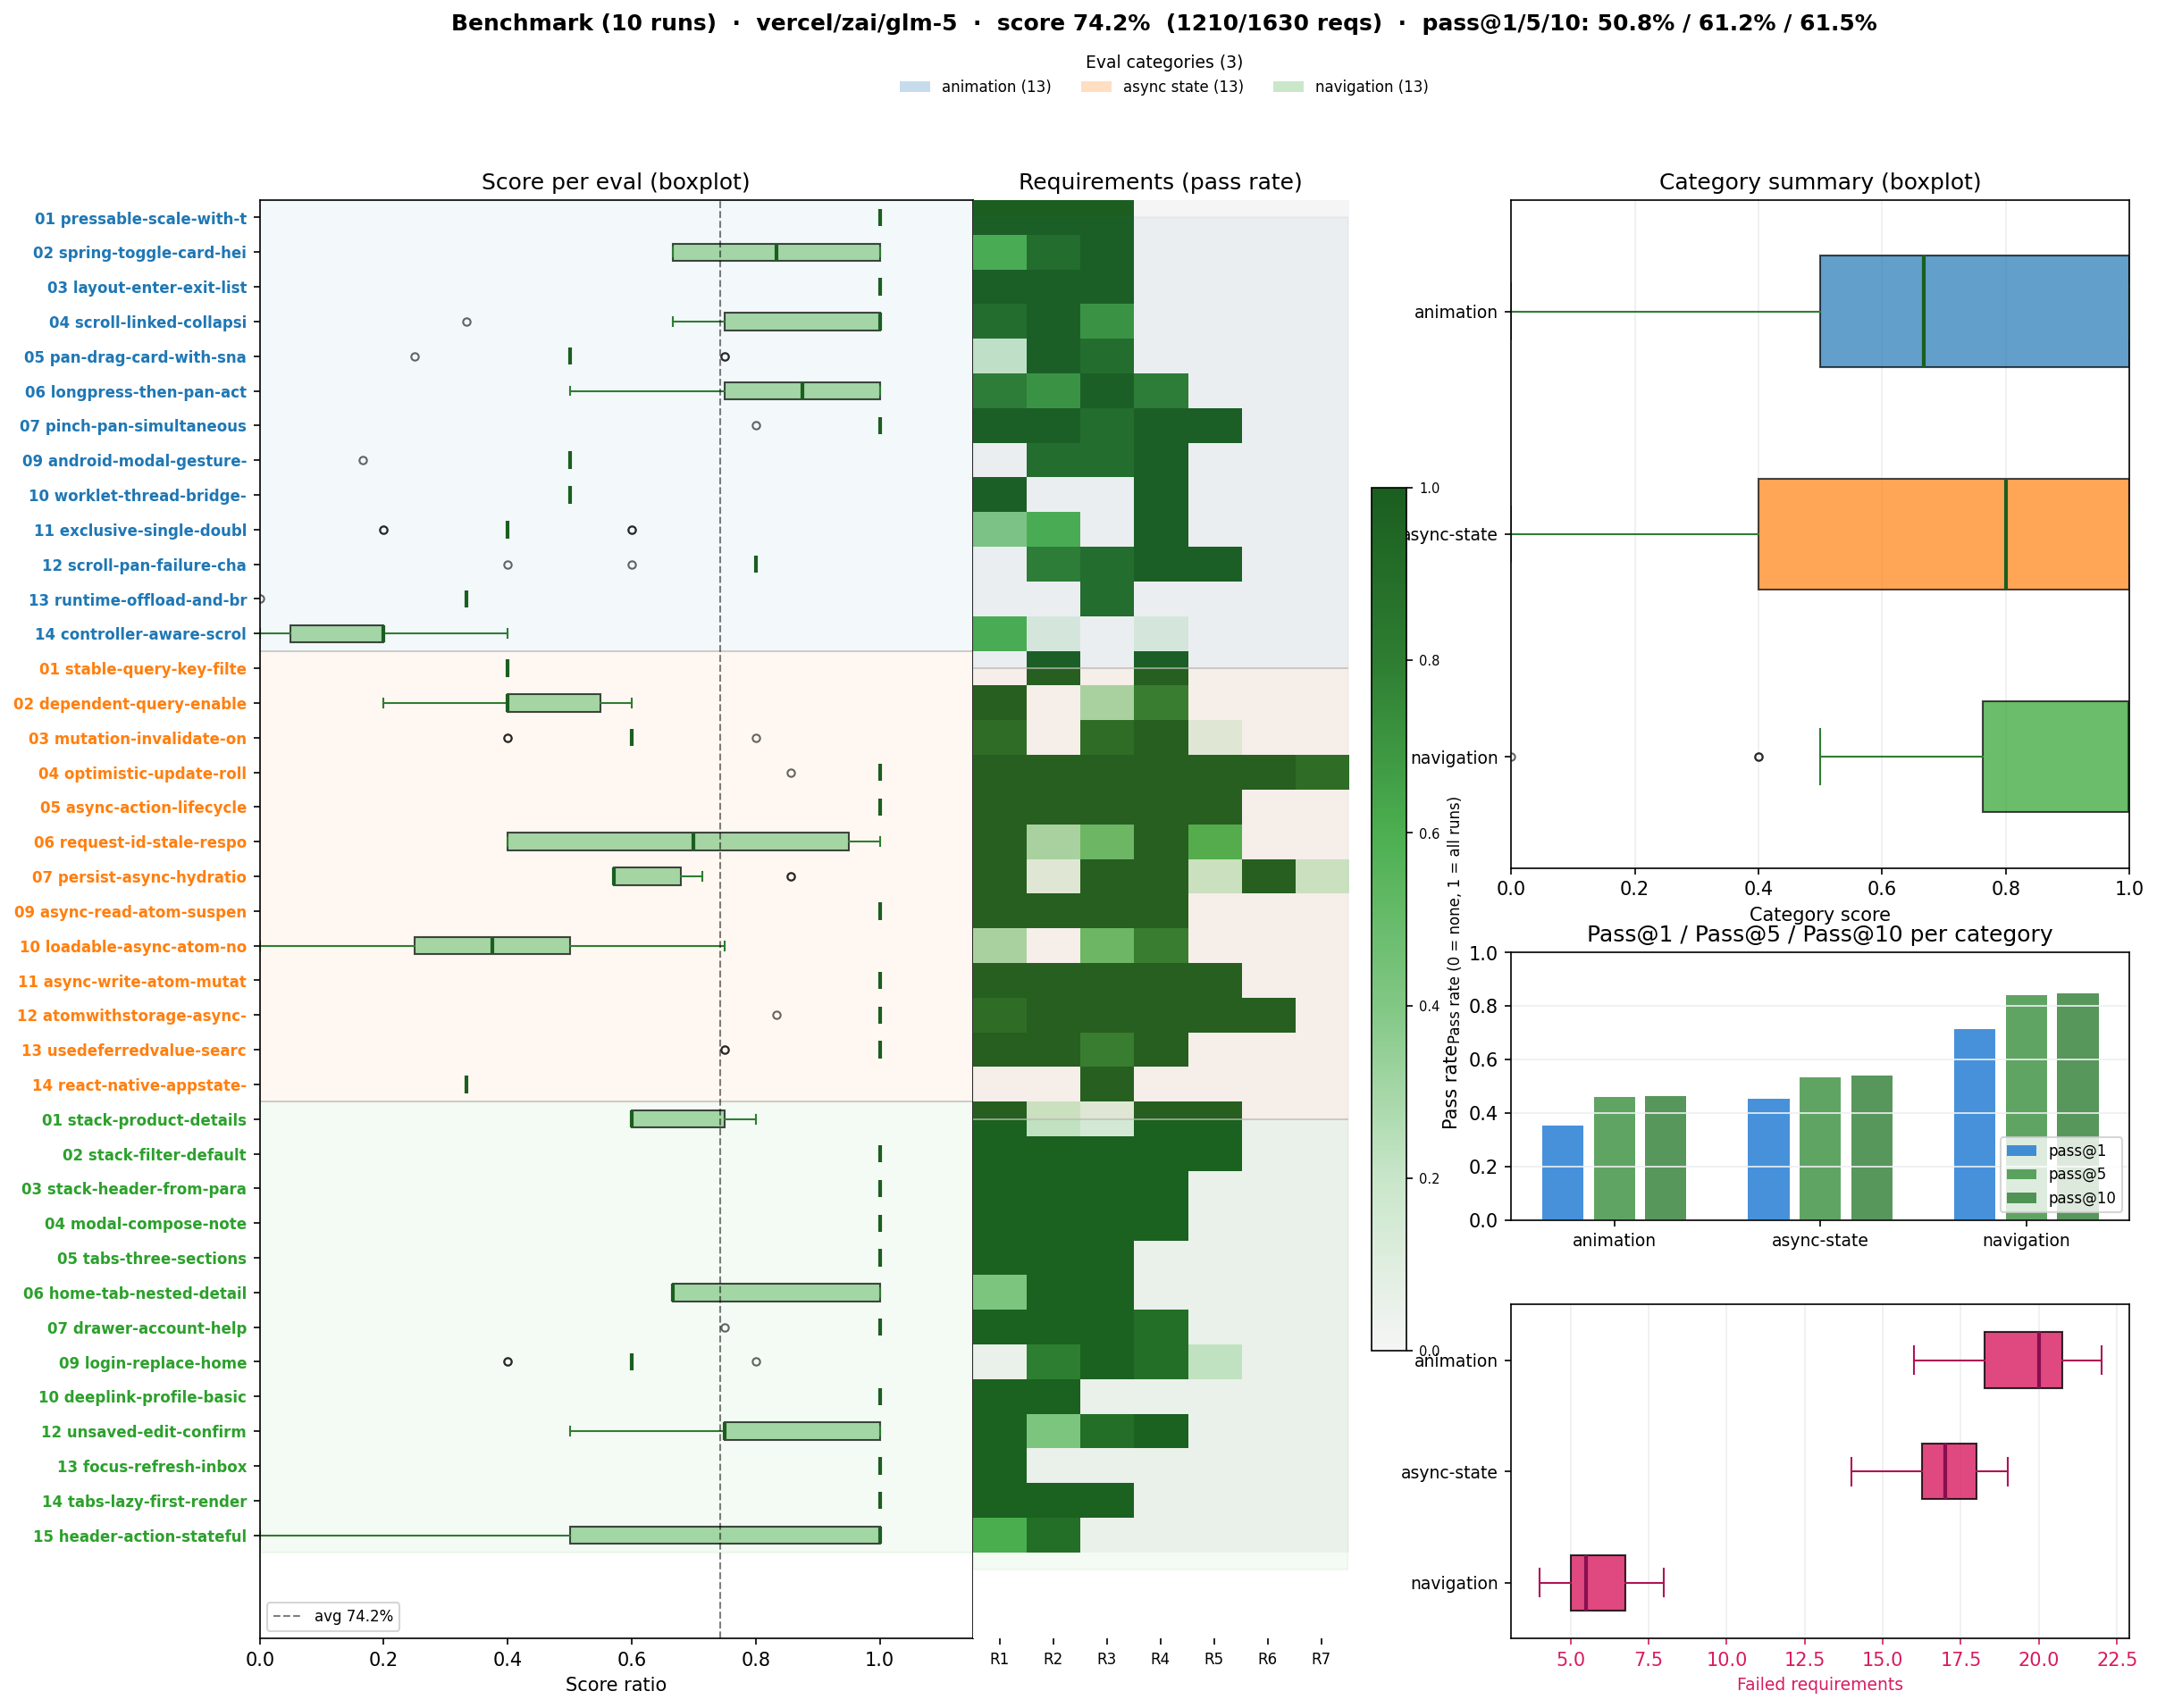
\includegraphics[width=\textwidth]{export/figures/glm-5_benchmark_plot.png}
\caption{Benchmark Plot for glm-5.}
\end{figure}

\begin{figure}[htbp]
\centering
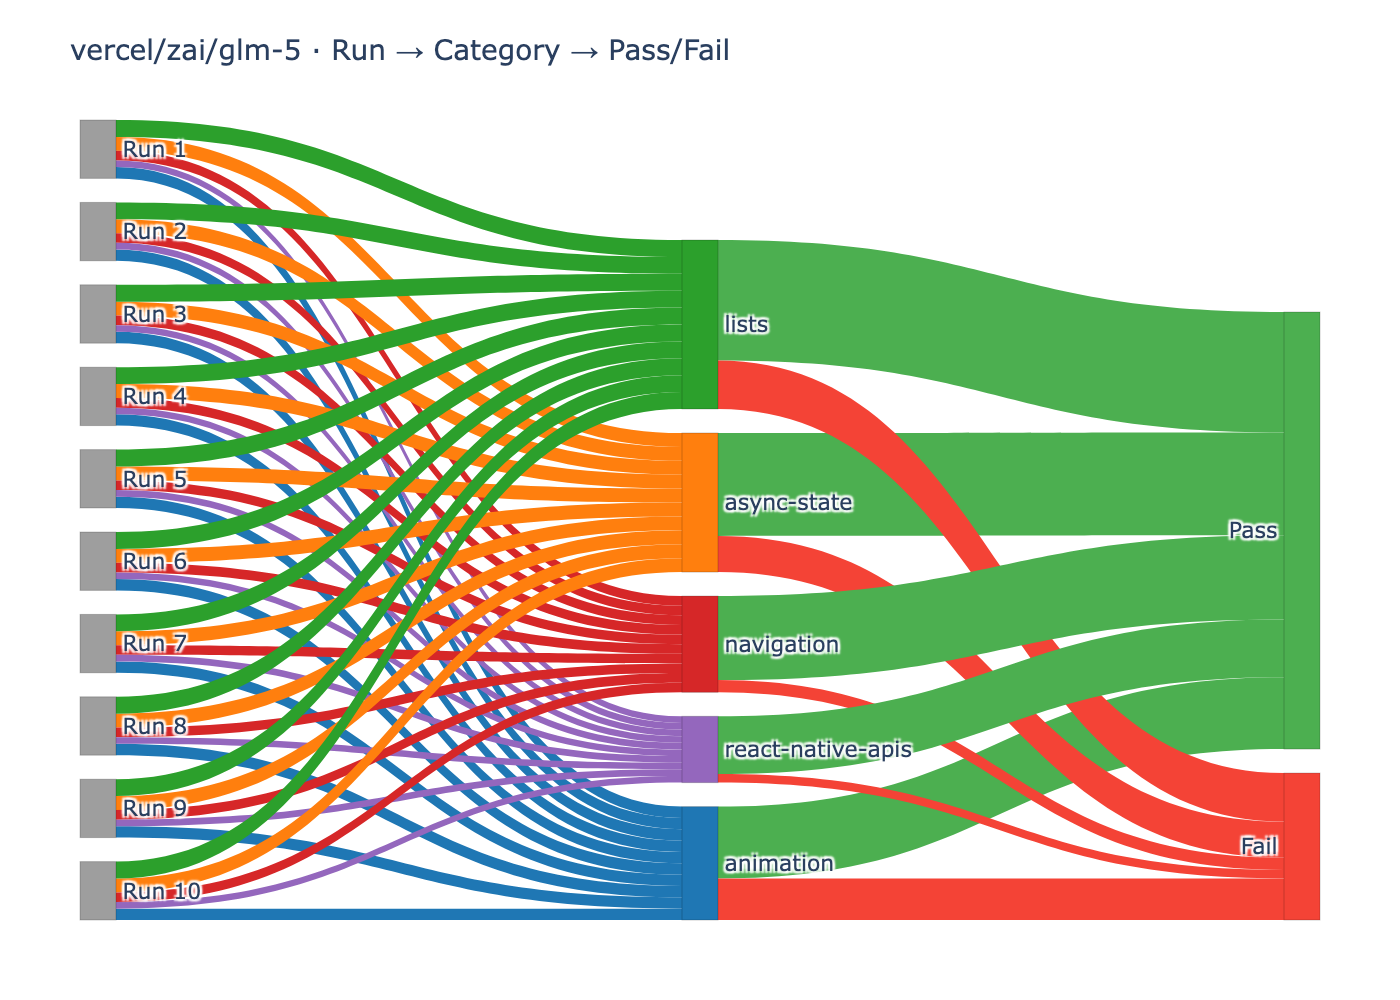
\includegraphics[width=\textwidth]{export/figures/glm-5_sankey_per_run.png}
\caption{Sankey per run for glm-5 showing the distribution of evals with respect to categories and results}
\end{figure}


\clearpage

\subsection{gpt-5.3-codex}

% Table: summary
% Requires: \usepackage{booktabs}
\begin{table}[htbp]
\centering
\begin{tabular}{lrrrrrr}
\toprule
Model & Runs & Score & Reqs & P@1 & P@5 & P@10 \\
\midrule
vercel/openai/gpt-5.3-codex & 10 & 83.1\% & 2267/2727 & 63.3\% & 74.5\% & 78.5\% \\
\bottomrule
\end{tabular}
\caption{Model summary for gpt-5.3-codex}
\end{table}


% Table: category_summary
% Requires: \usepackage{booktabs}
\begin{table}[htbp]
\centering
\begin{tabular}{lrrrr}
\toprule
Category & Score & Evals & Requirements & Failed requirements \\
\midrule
animation & 67.1\% & 130 & 53 & 186 \\
async state & 83.4\% & 129 & 65 & 105 \\
navigation & 96.2\% & 130 & 45 & 20 \\
\bottomrule
\end{tabular}
\caption{Results by category for gpt-5.3-codex. Score: mean(per-eval passed/total weight) across evals and runs. Evals: count of evaluation tasks. Requirements: sum of requirement count per eval. Failed requirements: sum of failed requirement instances across runs.}
\end{table}


% Table: per_eval
\input{export/tables/gpt-5.3-codex_per_eval}

\begin{figure}[htbp]
\centering
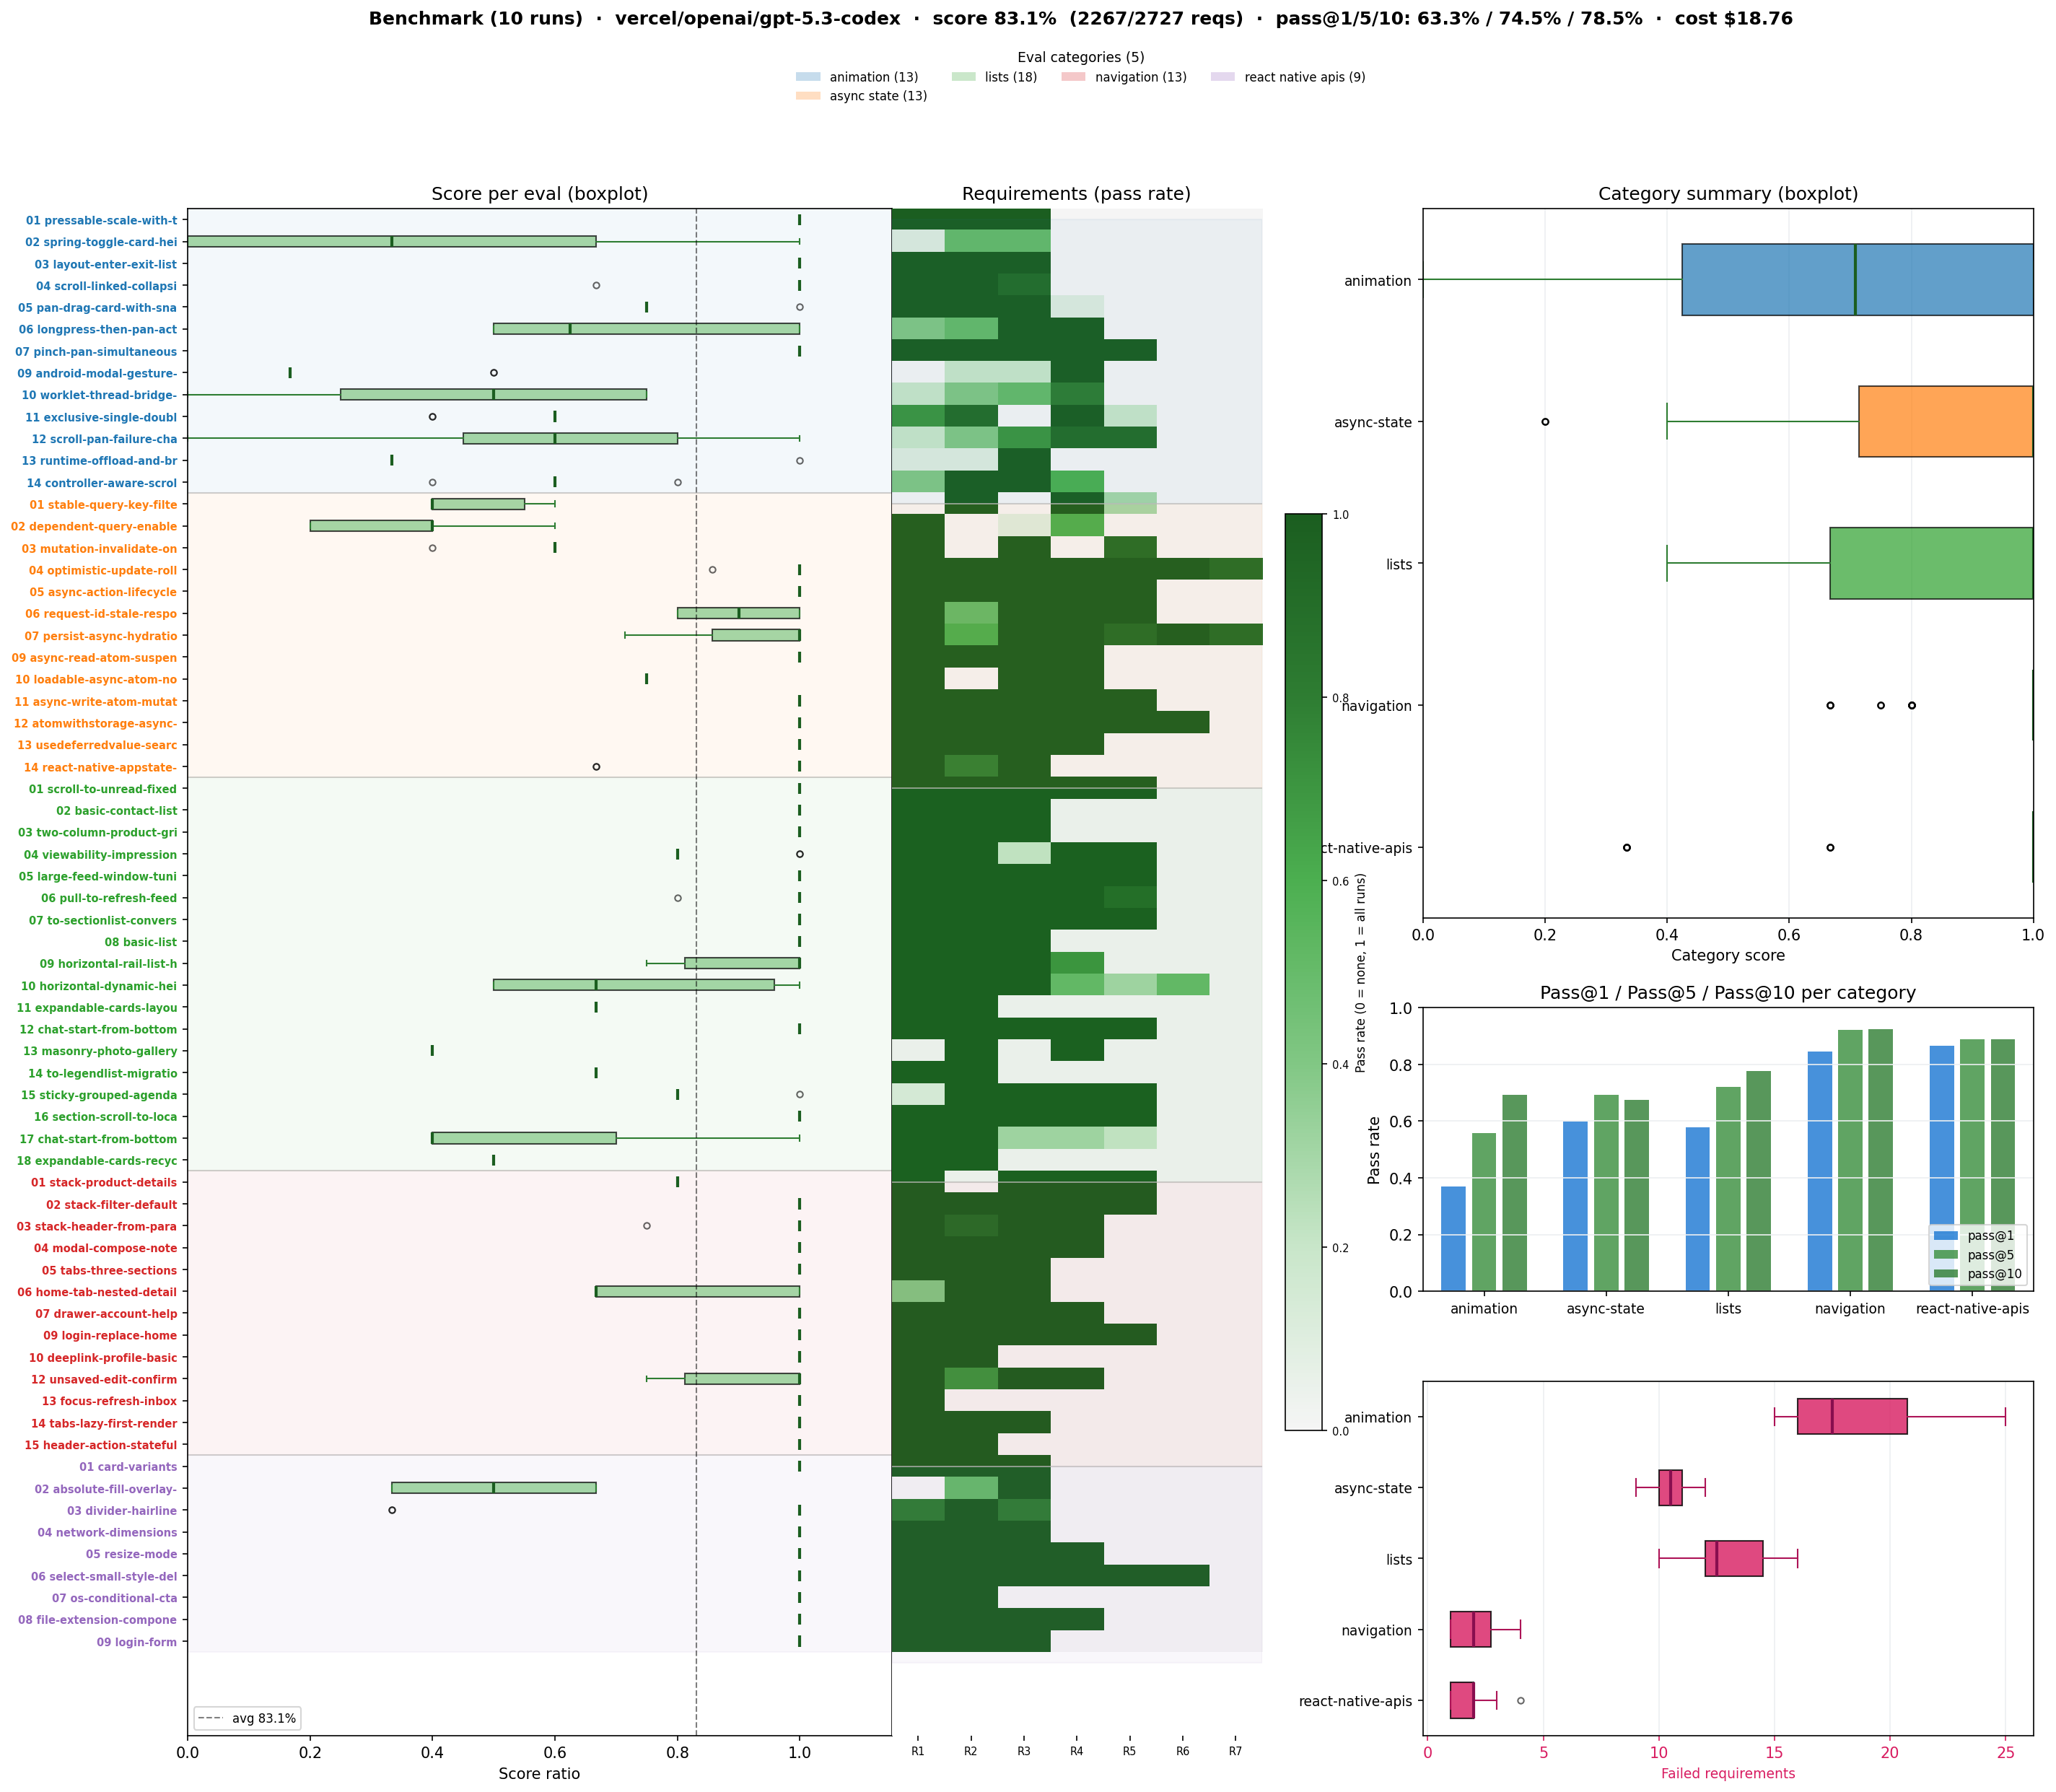
\includegraphics[width=\textwidth]{export/figures/gpt-5.3-codex_benchmark_plot.png}
\caption{Benchmark Plot for gpt-5.3-codex.}
\end{figure}

\begin{figure}[htbp]
\centering
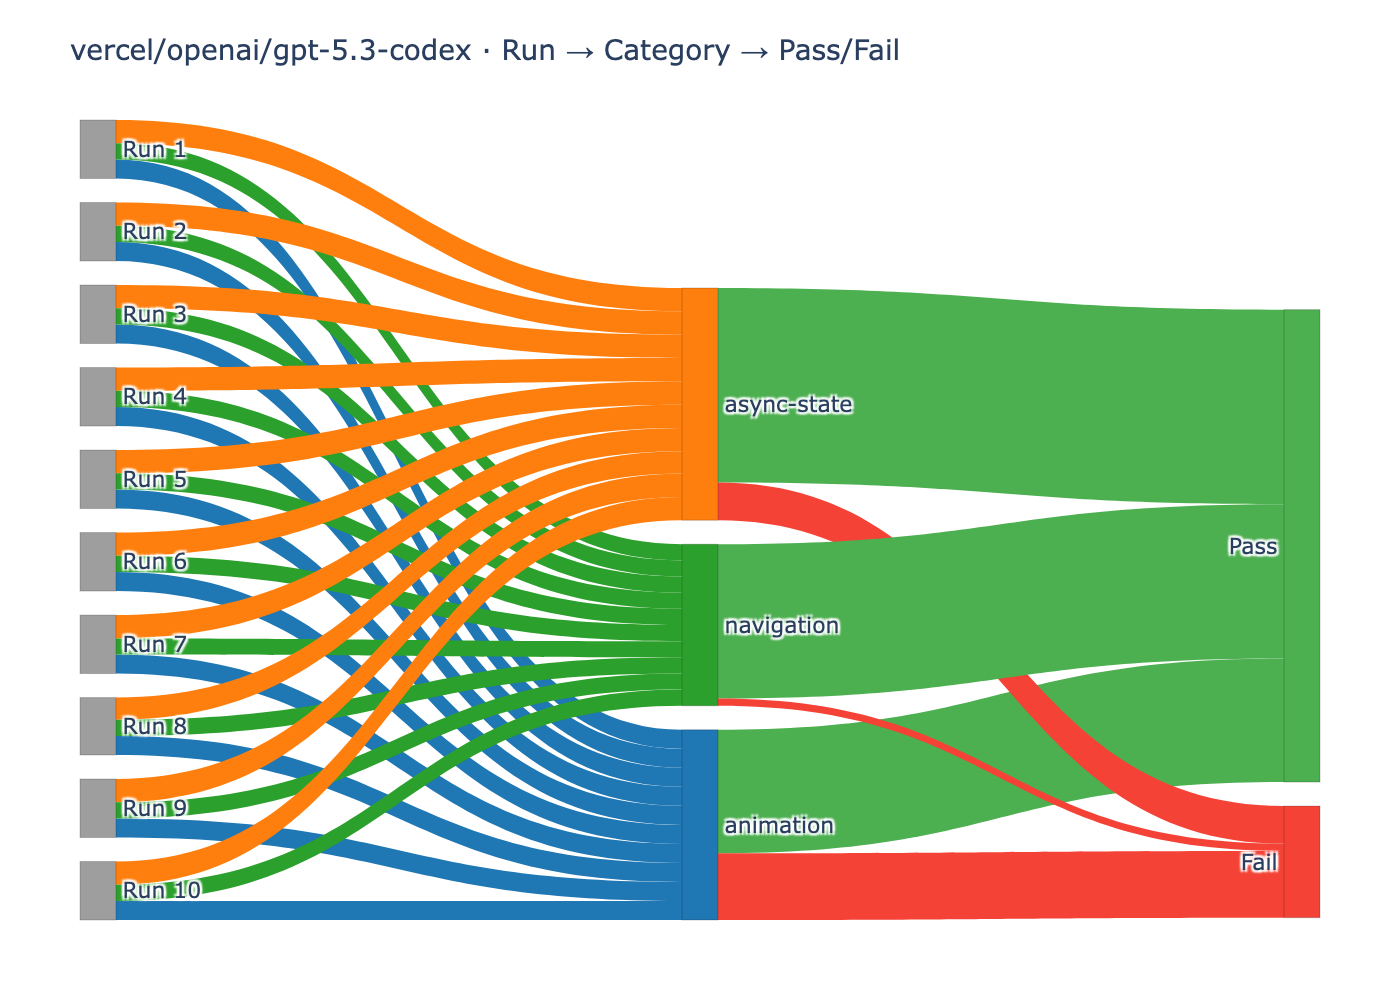
\includegraphics[width=\textwidth]{export/figures/gpt-5.3-codex_sankey_per_run.png}
\caption{Sankey per run for gpt-5.3-codex showing the distribution of evals with respect to categories and results}
\end{figure}


\clearpage

\subsection{gpt-5.4}

% Table: summary
% Requires: \usepackage{booktabs}
\begin{table}[htbp]
\centering
\begin{tabular}{lrrrrrr}
\toprule
Model & Runs & Score & Reqs & P@1 & P@5 & P@10 \\
\midrule
vercel/openai/gpt-5.4 & 10 & 85.3\% & 2330/2730 & 64.4\% & 74.7\% & 75.8\% \\
\bottomrule
\end{tabular}
\caption{Model summary for gpt-5.4}
\end{table}


% Table: category_summary
% Requires: \usepackage{booktabs}
\begin{table}[htbp]
\centering
\begin{tabular}{lrrrr}
\toprule
Category & Score & Evals & Requirements & Failed requirements \\
\midrule
animation & 71.3\% & 130 & 53 & 164 \\
async state & 85.6\% & 130 & 65 & 96 \\
navigation & 95.1\% & 130 & 45 & 23 \\
\bottomrule
\end{tabular}
\caption{Results by category for gpt-5.4. Score: mean(per-eval passed/total weight) across evals and runs. Evals: count of evaluation tasks. Requirements: sum of requirement count per eval. Failed requirements: sum of failed requirement instances across runs.}
\end{table}


% Table: per_eval
\input{export/tables/gpt-5.4_per_eval}

\begin{figure}[htbp]
\centering
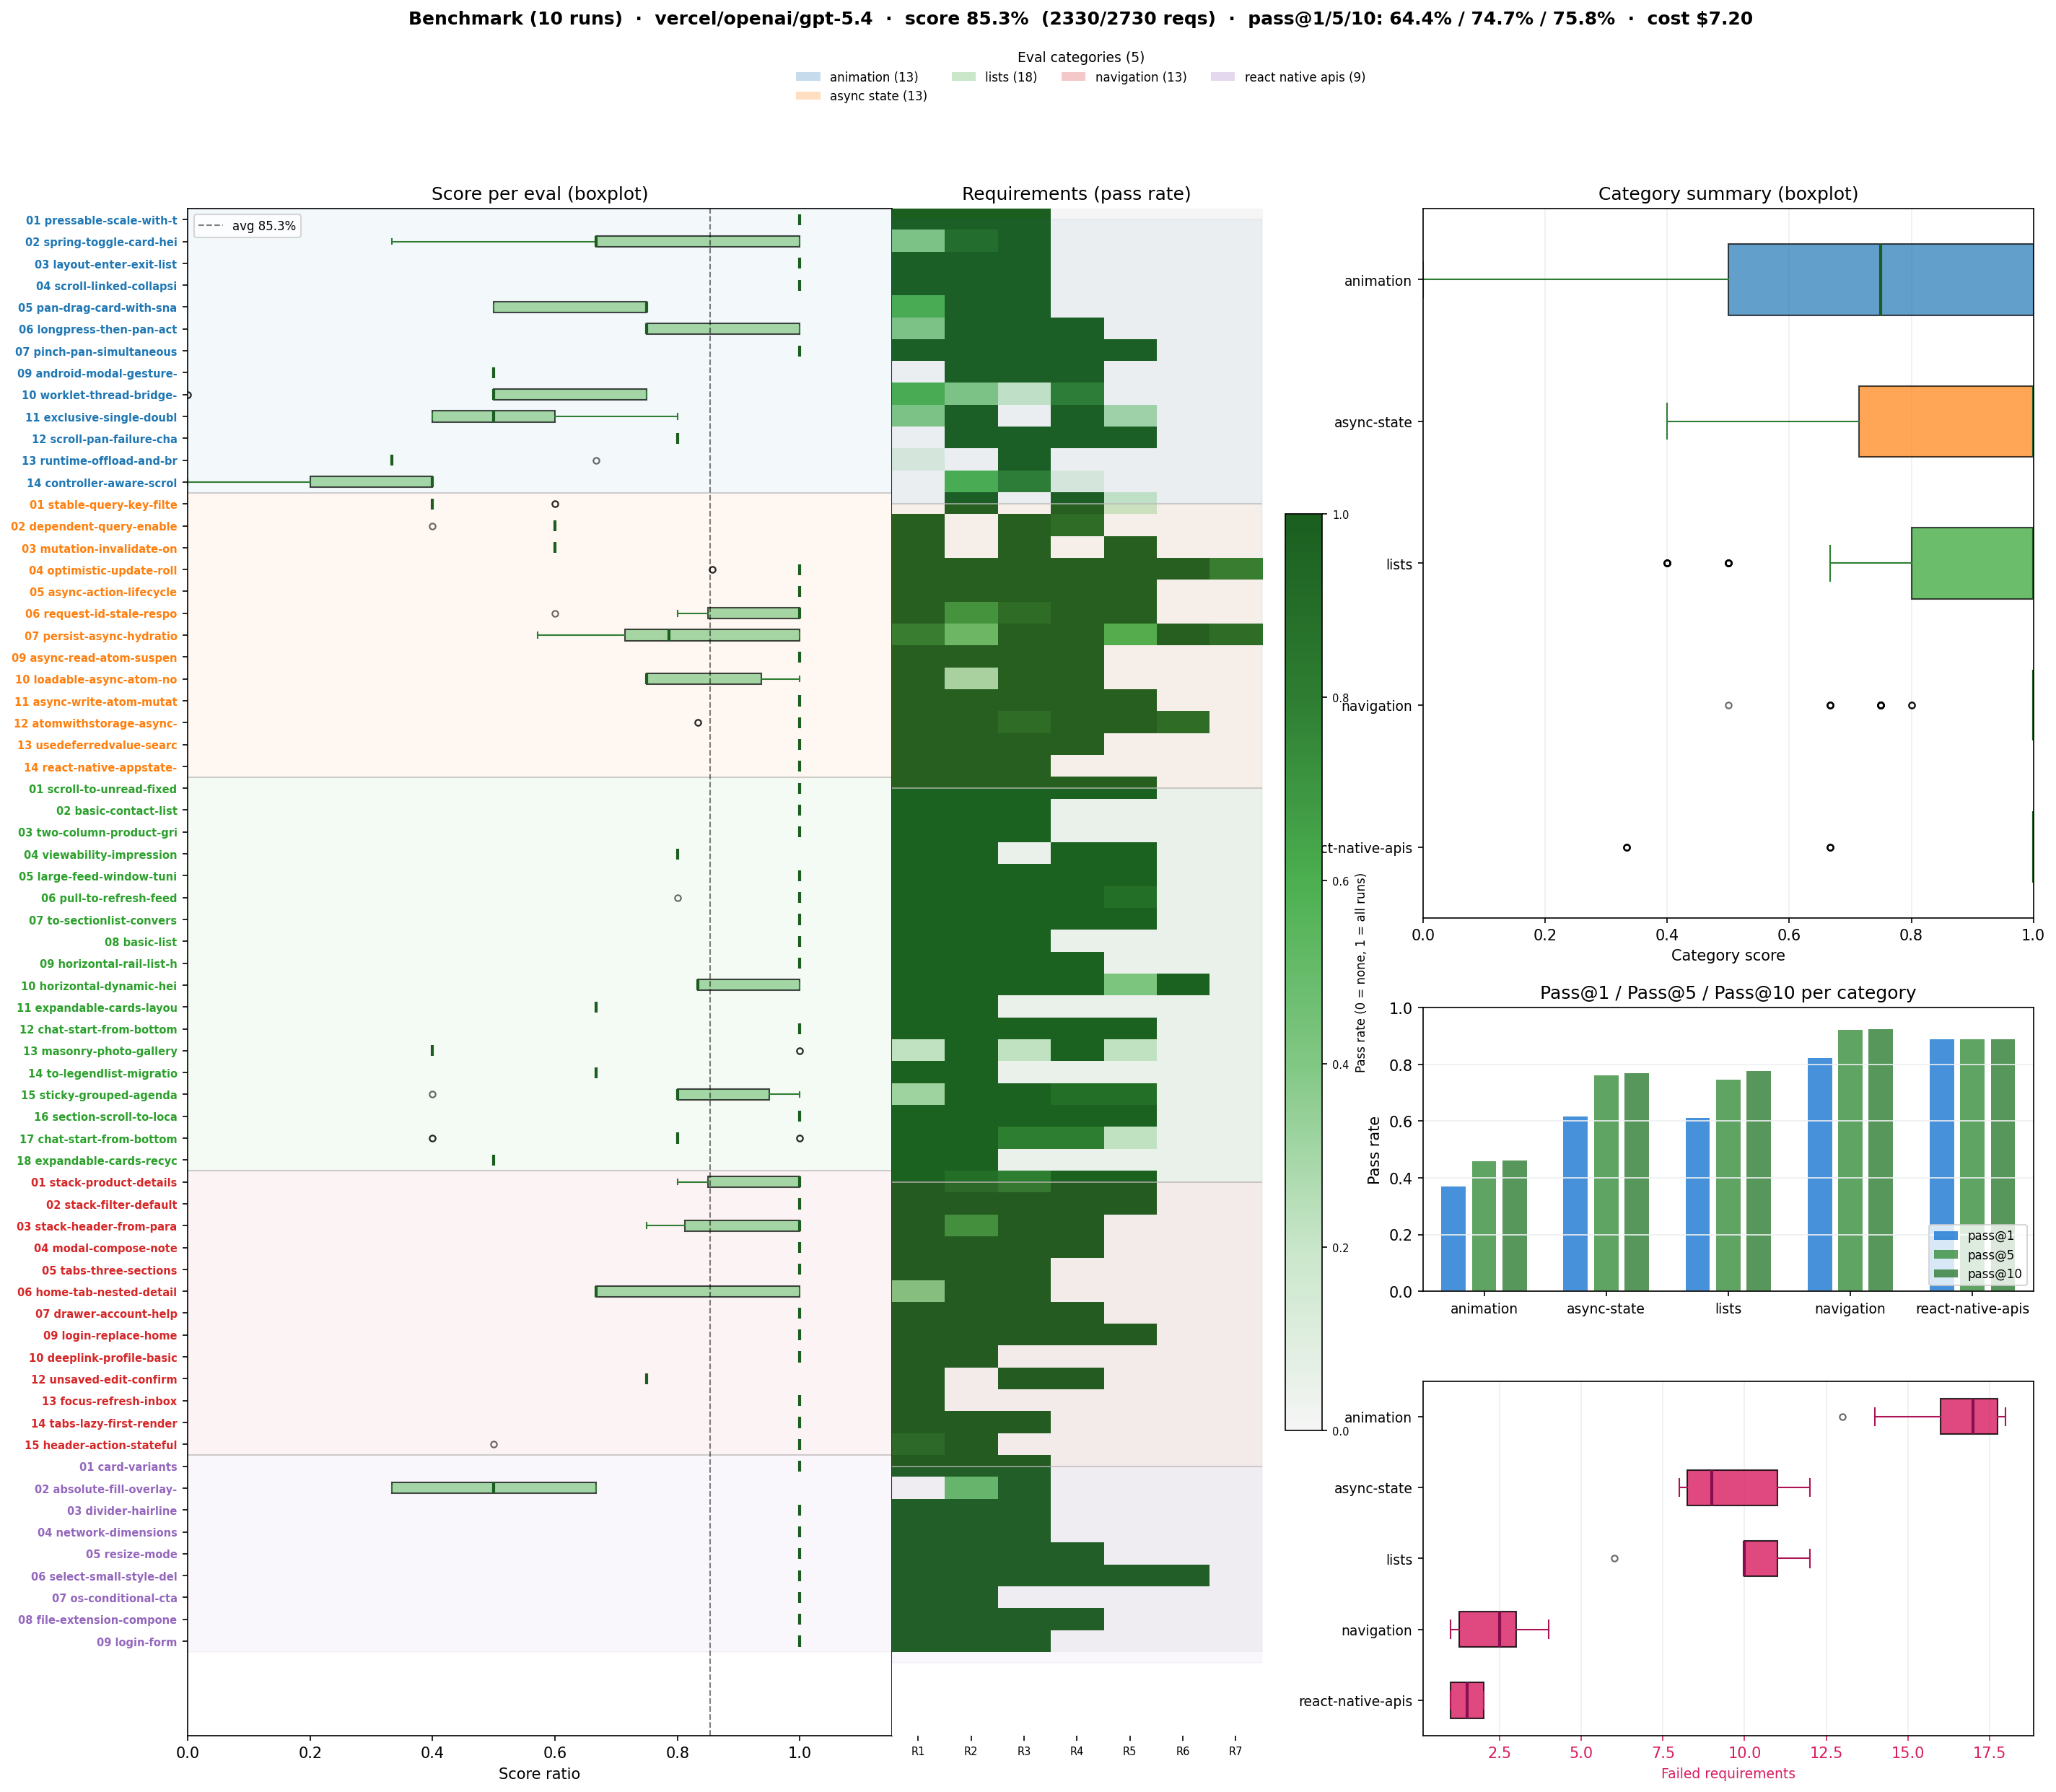
\includegraphics[width=\textwidth]{export/figures/gpt-5.4_benchmark_plot.png}
\caption{Benchmark Plot for gpt-5.4.}
\end{figure}

\begin{figure}[htbp]
\centering
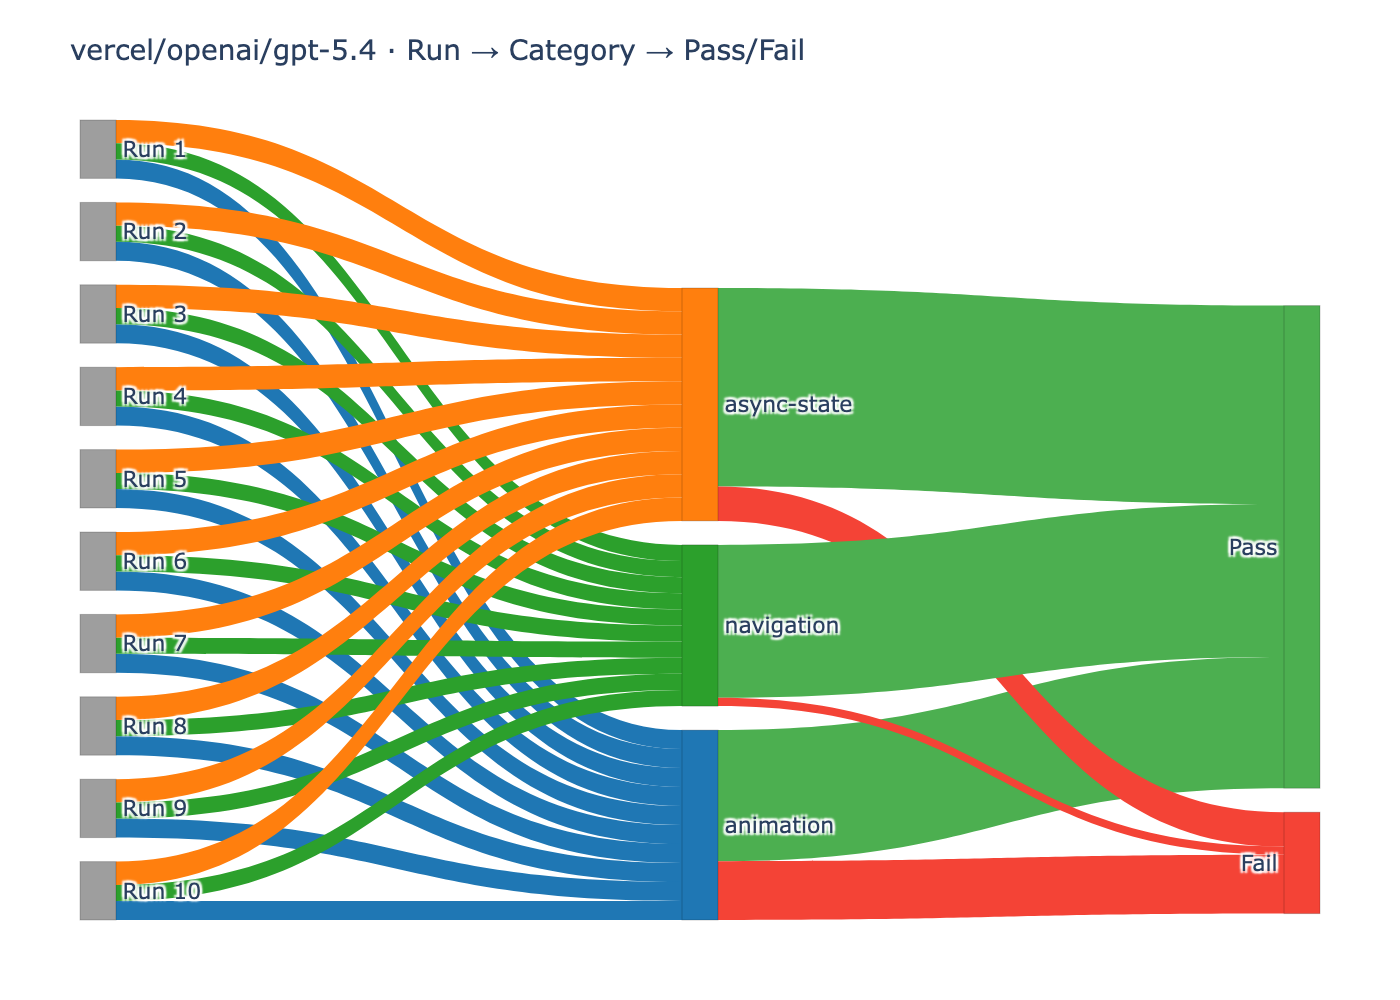
\includegraphics[width=\textwidth]{export/figures/gpt-5.4_sankey_per_run.png}
\caption{Sankey per run for gpt-5.4 showing the distribution of evals with respect to categories and results}
\end{figure}


\clearpage

\subsection{gpt-oss-120b}

% Table: summary
% Requires: \usepackage{booktabs}
\begin{table}[htbp]
\centering
\begin{tabular}{lrrrrrr}
\toprule
Model & Runs & Score & Reqs & P@1 & P@5 & P@10 \\
\midrule
cloudflare-ai-gateway/workers-ai/@cf/openai/gpt-os & 10 & 71.6\% & 1653/2308 & 46.0\% & 54.3\% & 50.4\% \\
\bottomrule
\end{tabular}
\caption{Model summary for gpt-oss-120b}
\end{table}


% Table: category_summary
% Requires: \usepackage{booktabs}
\begin{table}[htbp]
\centering
\begin{tabular}{lrrrr}
\toprule
Category & Score & Evals & Requirements & Failed requirements \\
\midrule
animation & 52.6\% & 110 & 53 & 239 \\
async state & 67.1\% & 129 & 65 & 204 \\
lists & 73.0\% & 122 & 79 & 144 \\
navigation & 88.5\% & 109 & 45 & 51 \\
react native apis & 93.7\% & 89 & 31 & 17 \\
\bottomrule
\end{tabular}
\caption{Results by category for gpt-oss-120b. Score: mean(per-eval passed/total weight) across evals and runs. Evals: count of evaluation tasks. Requirements: sum of requirement count per eval. Failed requirements: sum of failed requirement instances across runs.}
\end{table}


% Table: per_eval
% Requires: \usepackage{booktabs}
\begin{table}[htbp]
\centering
\begin{tabular}{lrrrrr}
\toprule
Eval & Category & Score & P@1 & P@5 & P@10 \\
\midrule
01-rn-anim-pressable-scale-with-timing & animation & 100.0\% & 100.0\% & 100.0\% & 100.0\% \\
02-rn-anim-spring-toggle-card-height & animation & 60.0\% & 0.0\% & 0.0\% & 0.0\% \\
03-rn-anim-layout-enter-exit-list-items & animation & 100.0\% & 100.0\% & 100.0\% & 100.0\% \\
04-rn-anim-scroll-linked-collapsing-header & animation & 100.0\% & 100.0\% & 100.0\% & 100.0\% \\
05-rn-anim-pan-drag-card-with-snap-points & animation & 25.0\% & 0.0\% & 0.0\% & 0.0\% \\
06-rn-anim-longpress-then-pan-activation-gate & animation & 45.0\% & 0.0\% & 0.0\% & 0.0\% \\
07-rn-anim-pinch-pan-simultaneous-photo-canvas & animation & 96.0\% & 80.0\% & 100.0\% & 80.0\% \\
09-rn-anim-android-modal-gesture-root-safety & animation & 16.7\% & 0.0\% & 0.0\% & 0.0\% \\
10-rn-anim-worklet-thread-bridge-schedule-on-rn & animation & 47.5\% & 0.0\% & 0.0\% & 0.0\% \\
11-rn-rngh-exclusive-single-double-tap & animation & 40.0\% & 0.0\% & 0.0\% & 0.0\% \\
12-rn-rngh-scroll-pan-failure-chain & animation & 12.0\% & 0.0\% & 0.0\% & 0.0\% \\
13-rn-worklets-runtime-offload-and-bridge & animation & 0.0\% & 0.0\% & 0.0\% & 0.0\% \\
14-rn-keyboard-controller-aware-scroll-footer & animation & 3.3\% & 0.0\% & 0.0\% & 0.0\% \\
01-rn-rq-stable-query-key-filters & async state & 20.0\% & 0.0\% & 0.0\% & 0.0\% \\
02-rn-rq-dependent-query-enabled-gate & async state & 40.0\% & 0.0\% & 0.0\% & 0.0\% \\
03-rn-rq-mutation-invalidate-on-success & async state & 36.0\% & 0.0\% & 0.0\% & 0.0\% \\
04-rn-rq-optimistic-update-rollback & async state & 84.3\% & 40.0\% & 97.6\% & 100.0\% \\
05-rn-zustand-async-action-lifecycle & async state & 100.0\% & 100.0\% & 100.0\% & 100.0\% \\
06-rn-zustand-request-id-stale-response-guard & async state & 88.0\% & 40.0\% & 97.6\% & 100.0\% \\
07-rn-zustand-persist-async-hydration-gate & async state & 54.3\% & 0.0\% & 0.0\% & 0.0\% \\
09-rn-jotai-async-read-atom-suspense & async state & 100.0\% & 100.0\% & 100.0\% & 100.0\% \\
10-rn-jotai-loadable-async-atom-no-suspense & async state & 27.5\% & 0.0\% & 0.0\% & 0.0\% \\
11-rn-jotai-async-write-atom-mutation & async state & 100.0\% & 100.0\% & 100.0\% & 100.0\% \\
12-rn-jotai-atomwithstorage-async-rehydrate-guard & async state & 96.7\% & 80.0\% & 100.0\% & 100.0\% \\
13-rn-react-usedeferredvalue-search-stale-indicator & async state & 94.4\% & 88.9\% & 100.0\% & 88.9\% \\
14-rn-rq-react-native-appstate-focus-online-managers & async state & 33.3\% & 0.0\% & 0.0\% & 0.0\% \\
01-rn-nav-stack-product-details & navigation & 73.3\% & 0.0\% & 0.0\% & 0.0\% \\
02-rn-nav-stack-filter-default & navigation & 100.0\% & 100.0\% & 100.0\% & 100.0\% \\
03-rn-nav-stack-header-from-param & navigation & 80.6\% & 22.2\% & 83.3\% & 22.2\% \\
04-rn-nav-modal-compose-note & navigation & 95.0\% & 80.0\% & 100.0\% & 100.0\% \\
05-rn-nav-tabs-three-sections & navigation & 72.2\% & 16.7\% & 83.3\% & 16.7\% \\
06-rn-nav-home-tab-nested-details & navigation & 96.3\% & 88.9\% & 100.0\% & 88.9\% \\
07-rn-nav-drawer-account-help & navigation & 87.5\% & 66.7\% & 100.0\% & 66.7\% \\
09-rn-nav-login-replace-home & navigation & 76.0\% & 0.0\% & 0.0\% & 0.0\% \\
10-rn-nav-deeplink-profile-basic & navigation & 100.0\% & 100.0\% & 100.0\% & 100.0\% \\
12-rn-nav-unsaved-edit-confirm & navigation & 62.5\% & 0.0\% & 0.0\% & 0.0\% \\
13-rn-nav-focus-refresh-inbox & navigation & 100.0\% & 100.0\% & 100.0\% & 100.0\% \\
14-rn-nav-tabs-lazy-first-render & navigation & 100.0\% & 100.0\% & 100.0\% & 100.0\% \\
15-rn-nav-header-action-stateful & navigation & 95.0\% & 90.0\% & 100.0\% & 100.0\% \\
\bottomrule
\end{tabular}
\caption{Per-eval results (score and pass@k) for gpt-oss-120b}
\end{table}


\begin{figure}[htbp]
\centering
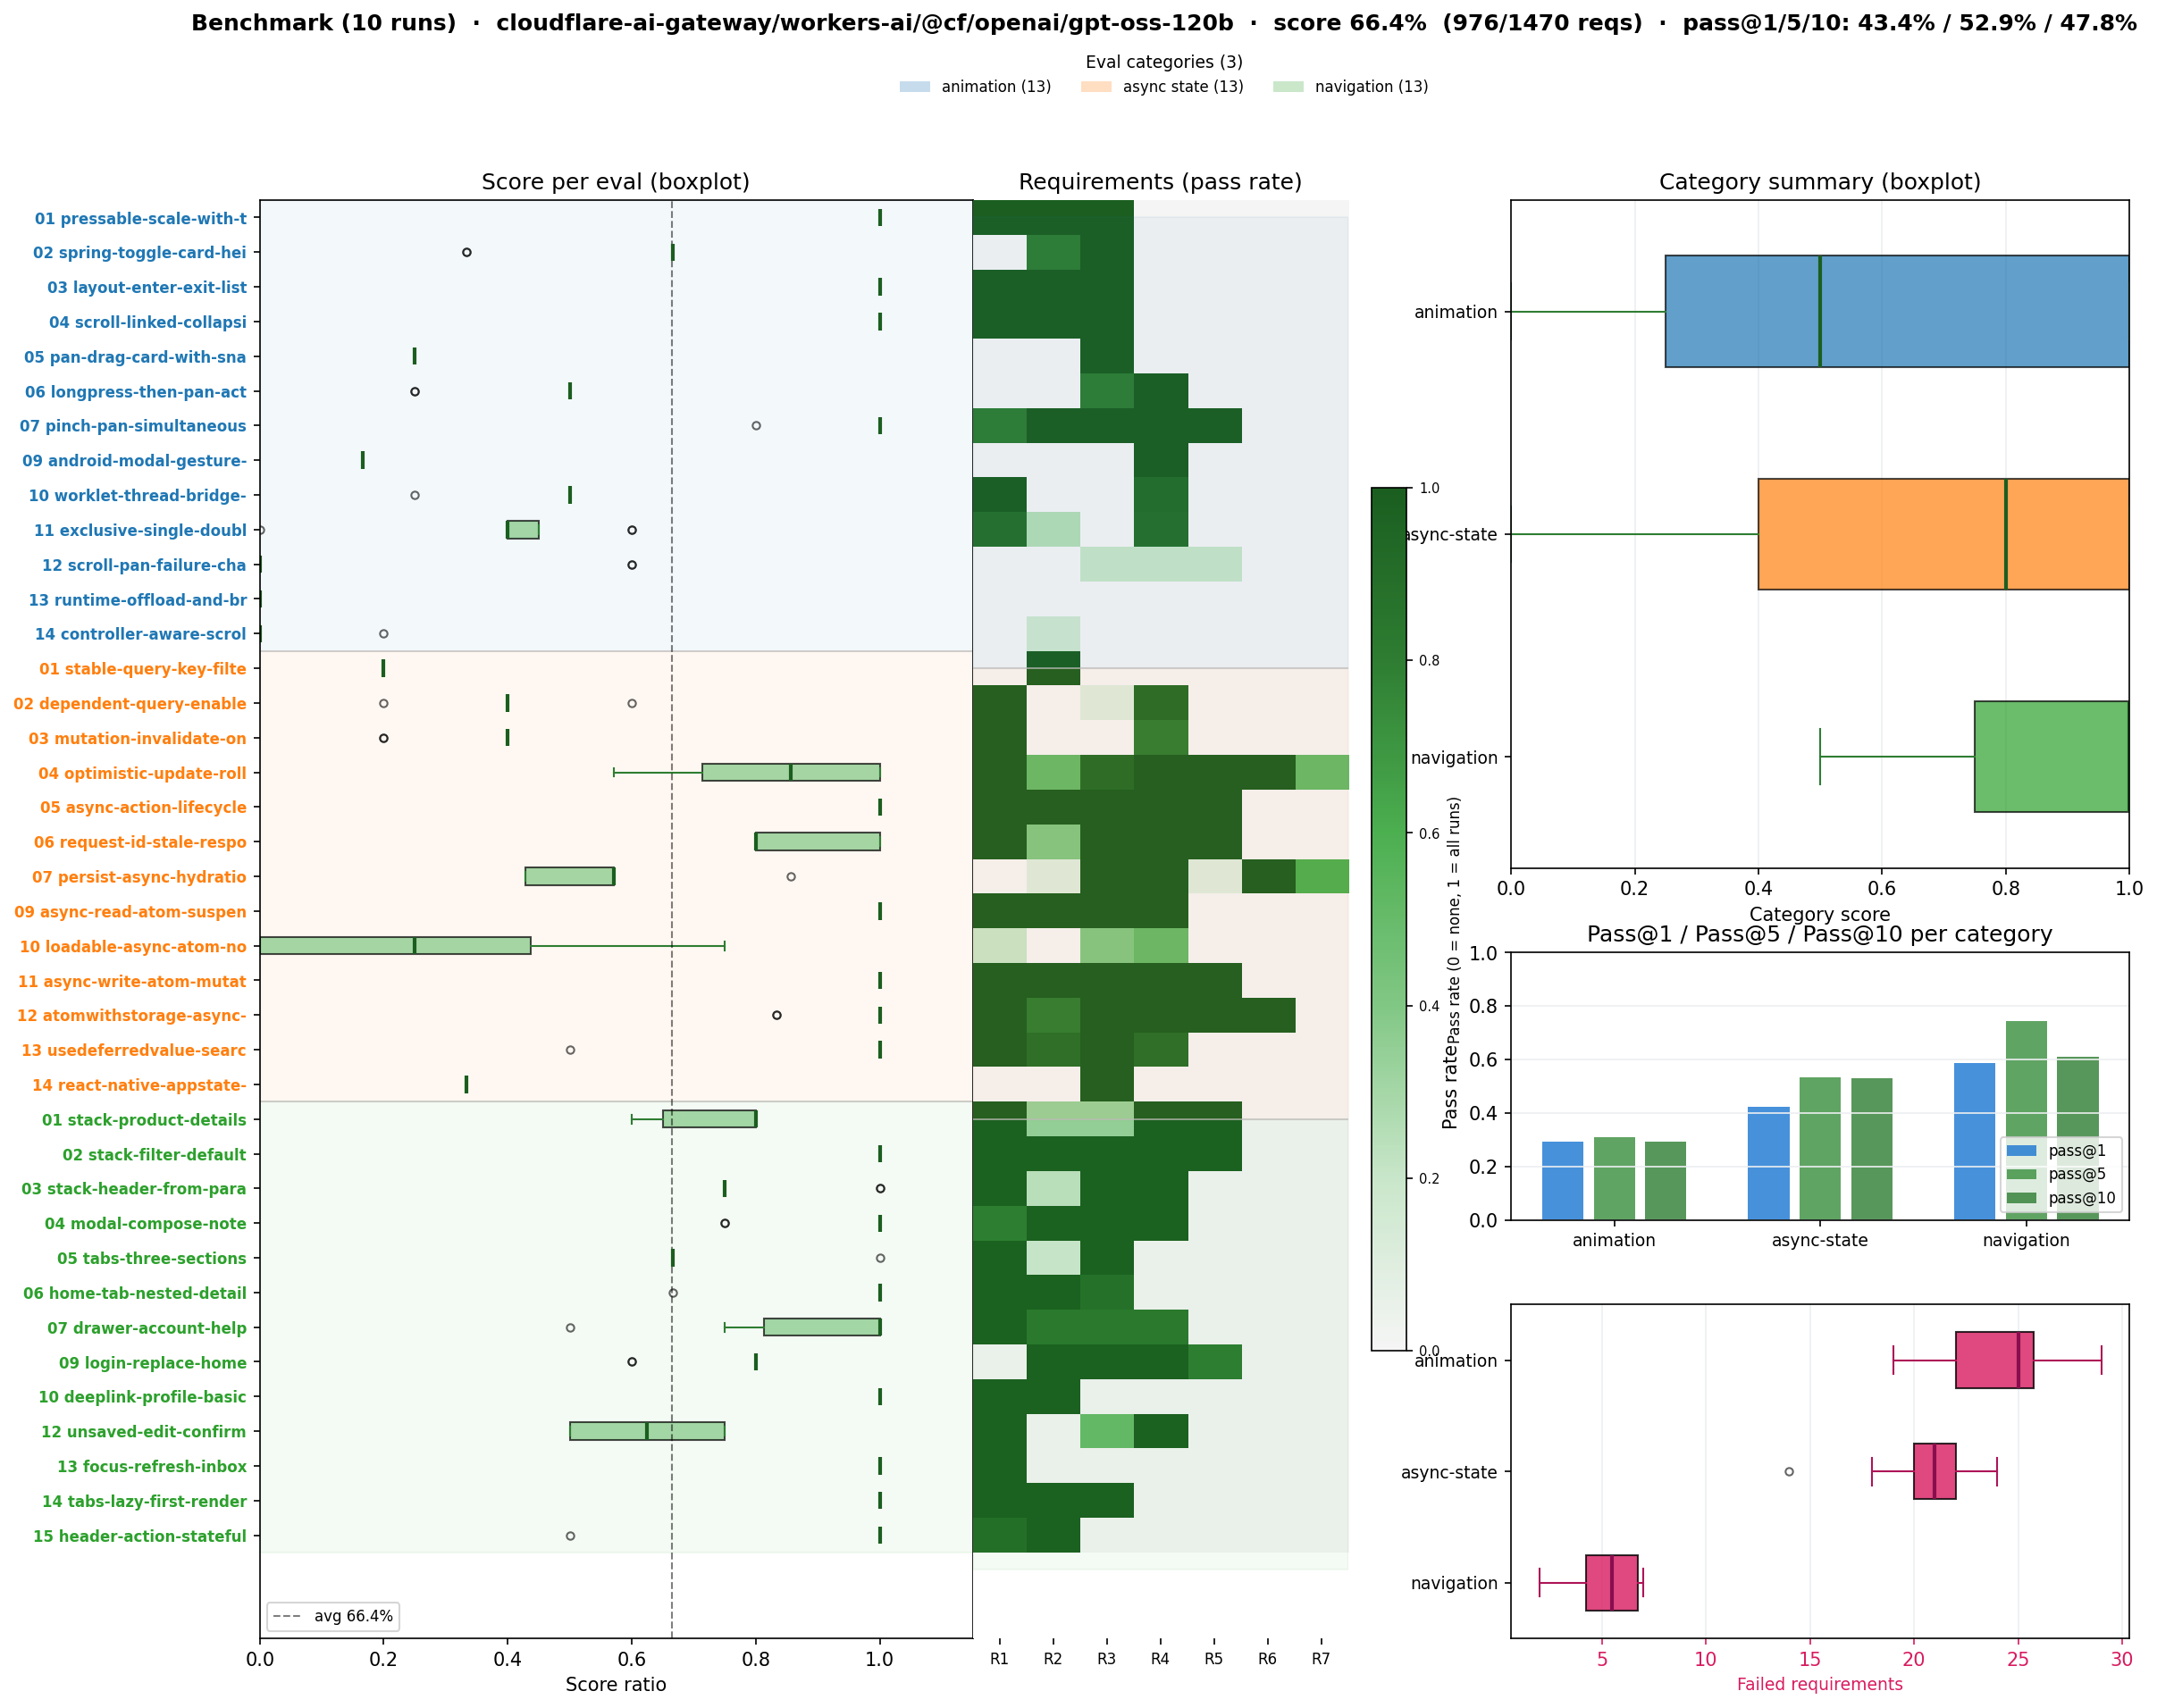
\includegraphics[width=\textwidth]{export/figures/gpt-oss-120b_benchmark_plot.png}
\caption{Benchmark Plot for gpt-oss-120b.}
\end{figure}

\begin{figure}[htbp]
\centering
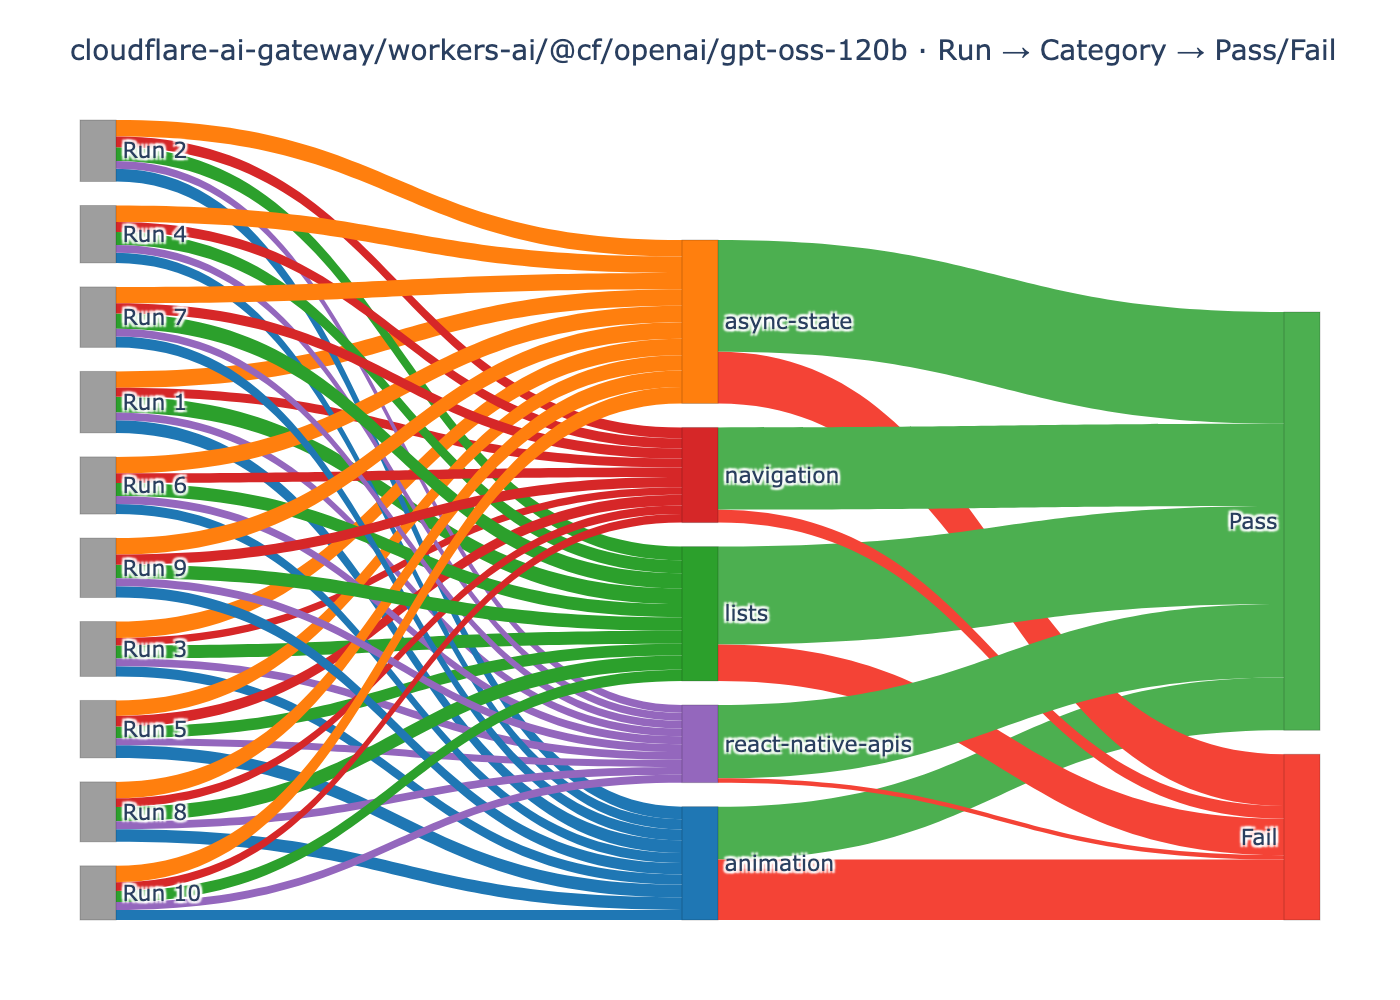
\includegraphics[width=\textwidth]{export/figures/gpt-oss-120b_sankey_per_run.png}
\caption{Sankey per run for gpt-oss-120b showing the distribution of evals with respect to categories and results}
\end{figure}


\clearpage

\subsection{gpt-oss-20b}

% Table: summary
% Requires: \usepackage{booktabs}
\begin{table}[htbp]
\centering
\begin{tabular}{lrrrrrr}
\toprule
Model & Runs & Score & Reqs & P@1 & P@5 & P@10 \\
\midrule
cloudflare-ai-gateway/workers-ai/@cf/openai/gpt-os & 10 & 71.0\% & 1761/2480 & 43.4\% & 56.2\% & 55.4\% \\
\bottomrule
\end{tabular}
\caption{Model summary for gpt-oss-20b}
\end{table}


% Table: category_summary
% Requires: \usepackage{booktabs}
\begin{table}[htbp]
\centering
\begin{tabular}{lrrrr}
\toprule
Category & Score & Evals & Requirements & Failed requirements \\
\midrule
animation & 51.7\% & 107 & 53 & 232 \\
async state & 65.8\% & 128 & 65 & 212 \\
navigation & 84.2\% & 94 & 45 & 61 \\
\bottomrule
\end{tabular}
\caption{Results by category for gpt-oss-20b. Score: mean(per-eval passed/total weight) across evals and runs. Evals: count of evaluation tasks. Requirements: sum of requirement count per eval. Failed requirements: sum of failed requirement instances across runs.}
\end{table}


% Table: per_eval
\input{export/tables/gpt-oss-20b_per_eval}

\begin{figure}[htbp]
\centering
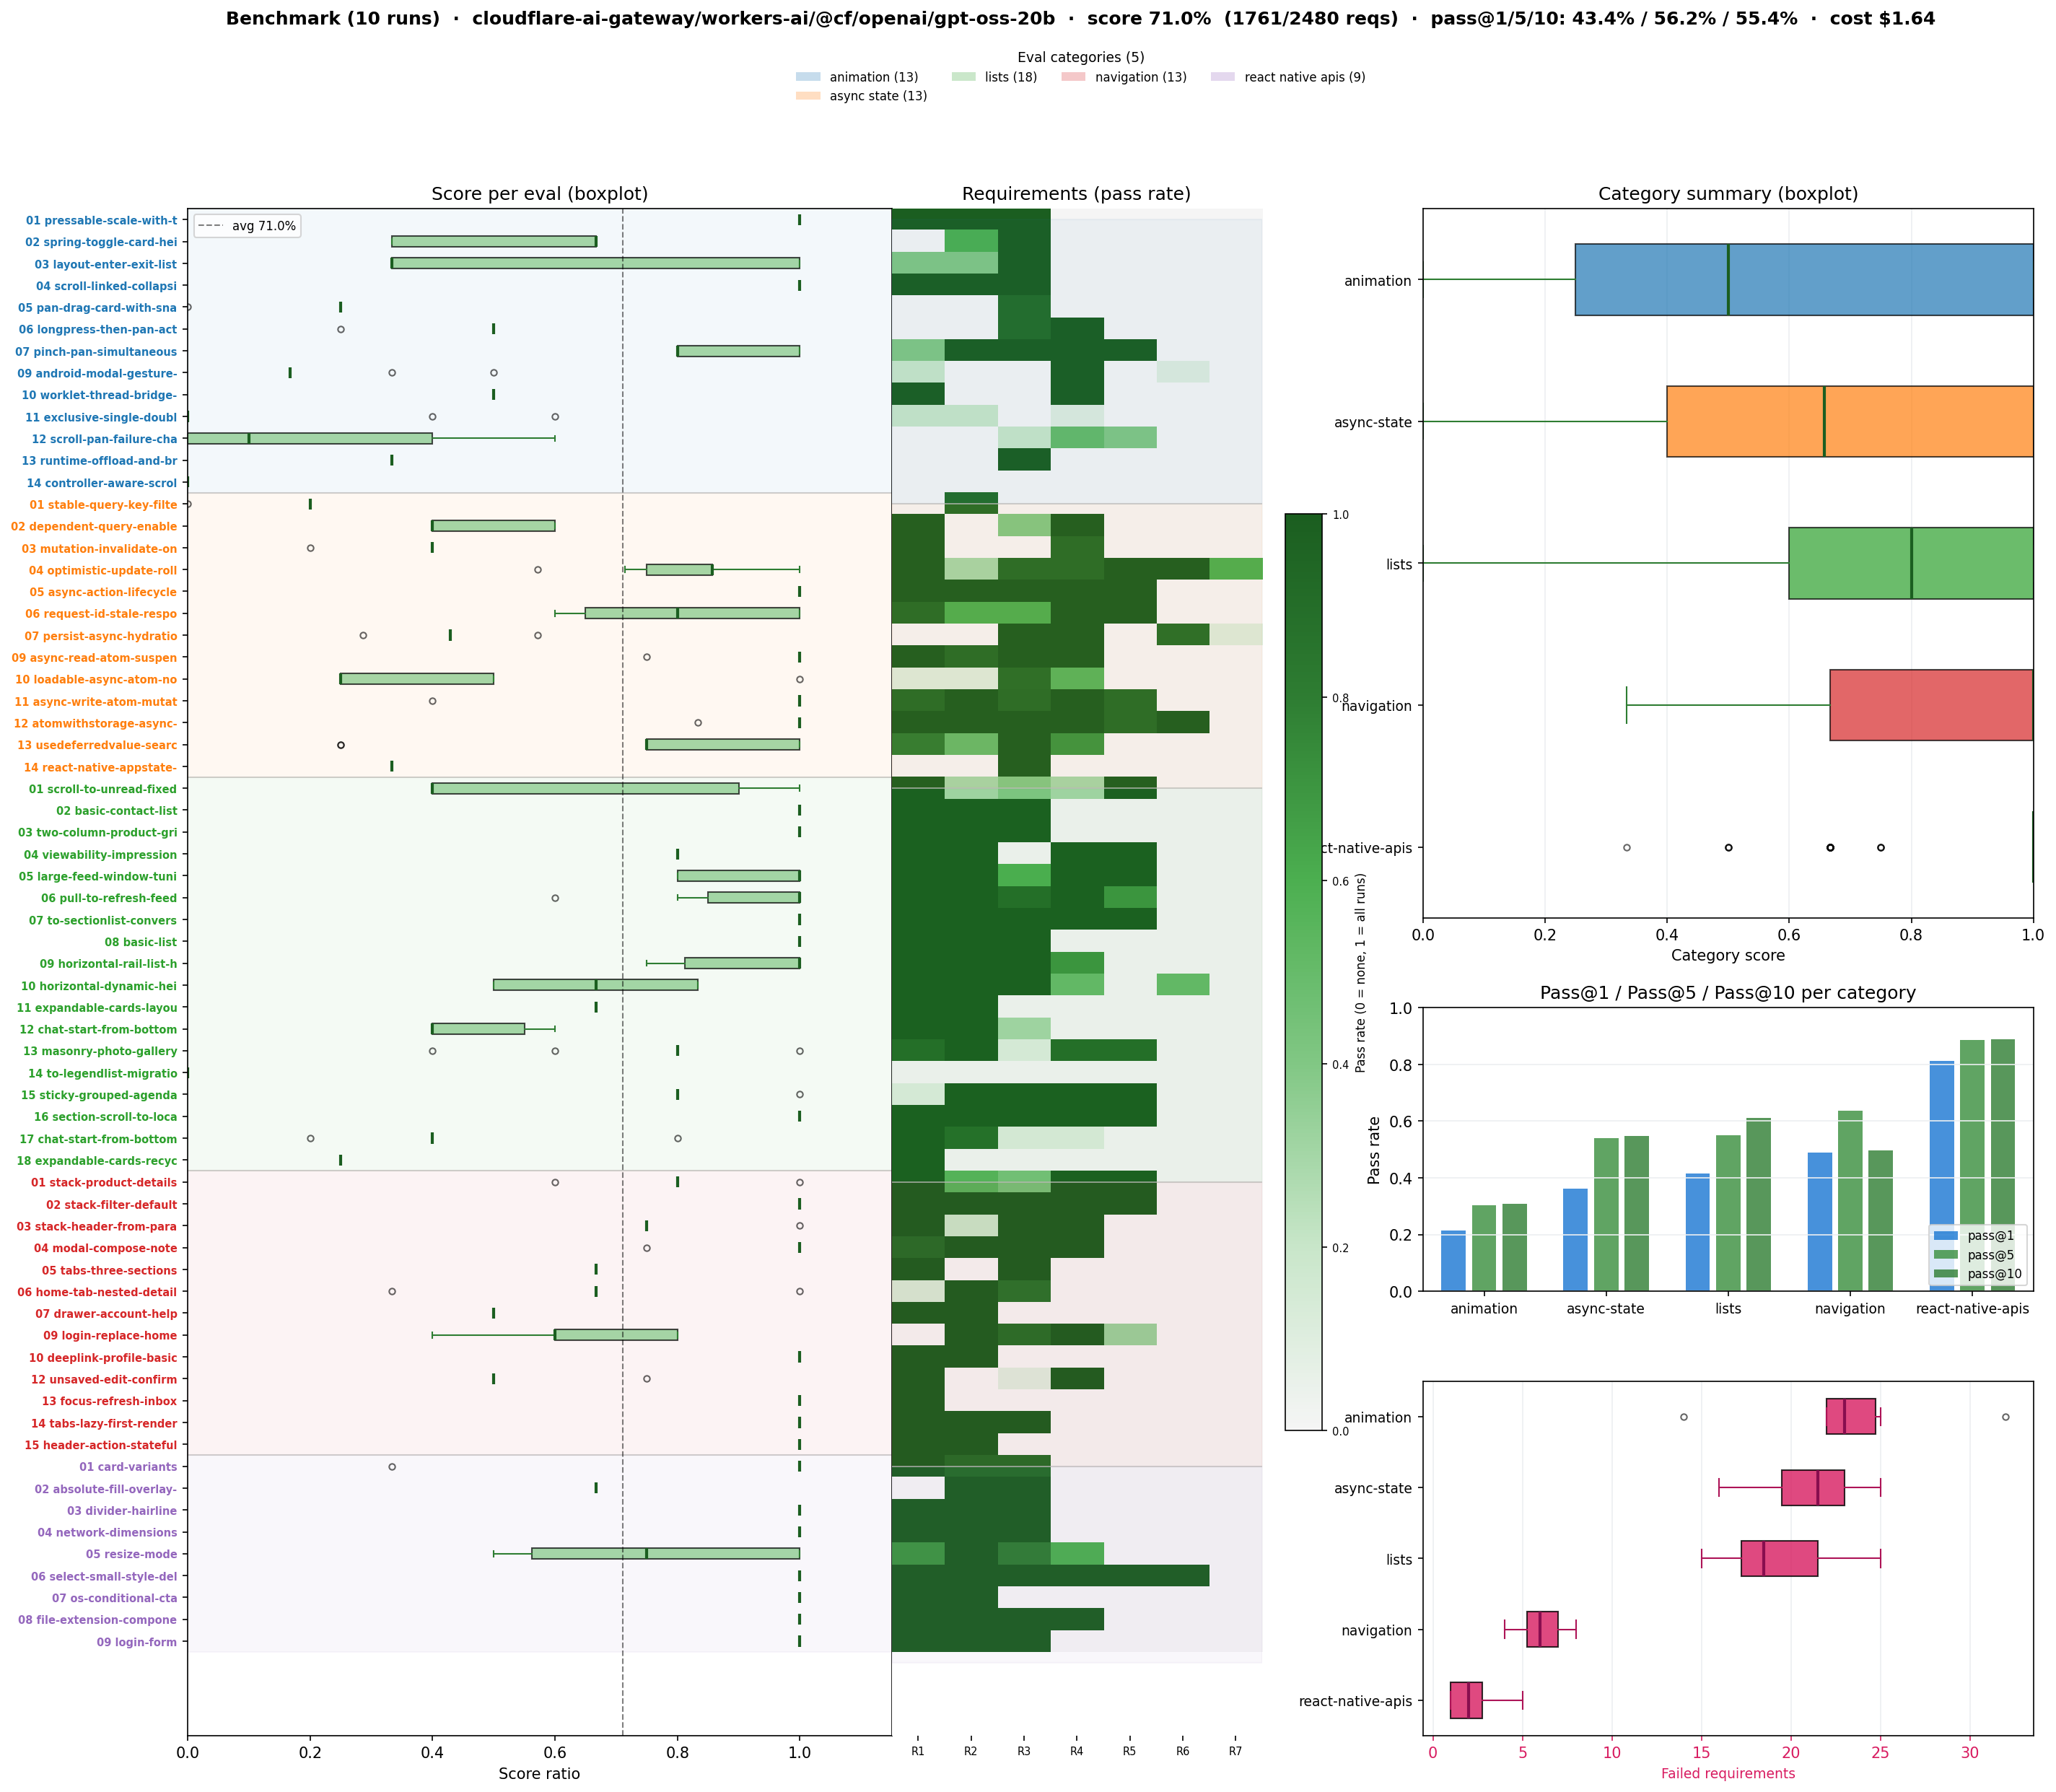
\includegraphics[width=\textwidth]{export/figures/gpt-oss-20b_benchmark_plot.png}
\caption{Benchmark Plot for gpt-oss-20b.}
\end{figure}

\begin{figure}[htbp]
\centering
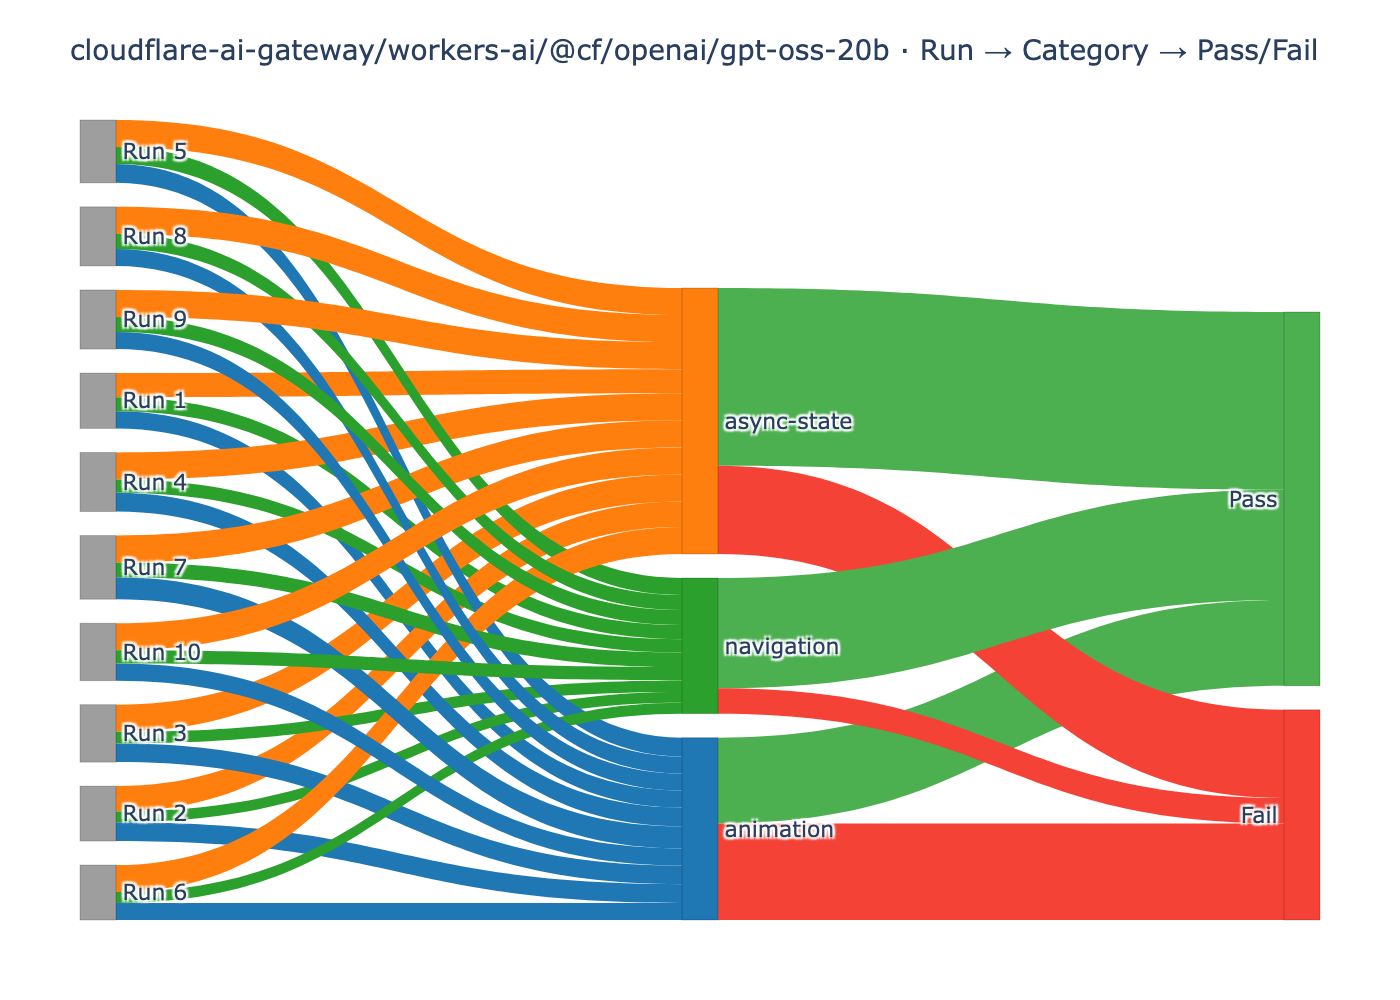
\includegraphics[width=\textwidth]{export/figures/gpt-oss-20b_sankey_per_run.png}
\caption{Sankey per run for gpt-oss-20b showing the distribution of evals with respect to categories and results}
\end{figure}


\clearpage

\subsection{grok-4}

% Table: summary
% Requires: \usepackage{booktabs}
\begin{table}[htbp]
\centering
\begin{tabular}{lrrrrrr}
\toprule
Model & Runs & Score & Reqs & P@1 & P@5 & P@10 \\
\midrule
vercel/xai/grok-4 & 10 & 70.1\% & 1142/1630 & 40.3\% & 50.3\% & 51.3\% \\
\bottomrule
\end{tabular}
\caption{Model summary for grok-4}
\end{table}


% Table: category_summary
% Requires: \usepackage{booktabs}
\begin{table}[htbp]
\centering
\begin{tabular}{lrrrr}
\toprule
Category & Score & Evals & Requirements & Failed requirements \\
\midrule
animation & 60.7\% & 130 & 53 & 226 \\
async state & 70.1\% & 130 & 65 & 187 \\
lists & 69.6\% & 180 & 79 & 237 \\
navigation & 84.9\% & 130 & 45 & 75 \\
react native apis & 92.1\% & 89 & 31 & 21 \\
\bottomrule
\end{tabular}
\caption{Results by category for grok-4. Score: mean(per-eval passed/total weight) across evals and runs. Evals: count of evaluation tasks. Requirements: sum of requirement count per eval. Failed requirements: sum of failed requirement instances across runs.}
\end{table}


% Table: per_eval
\input{export/tables/grok-4_per_eval}

\begin{figure}[htbp]
\centering
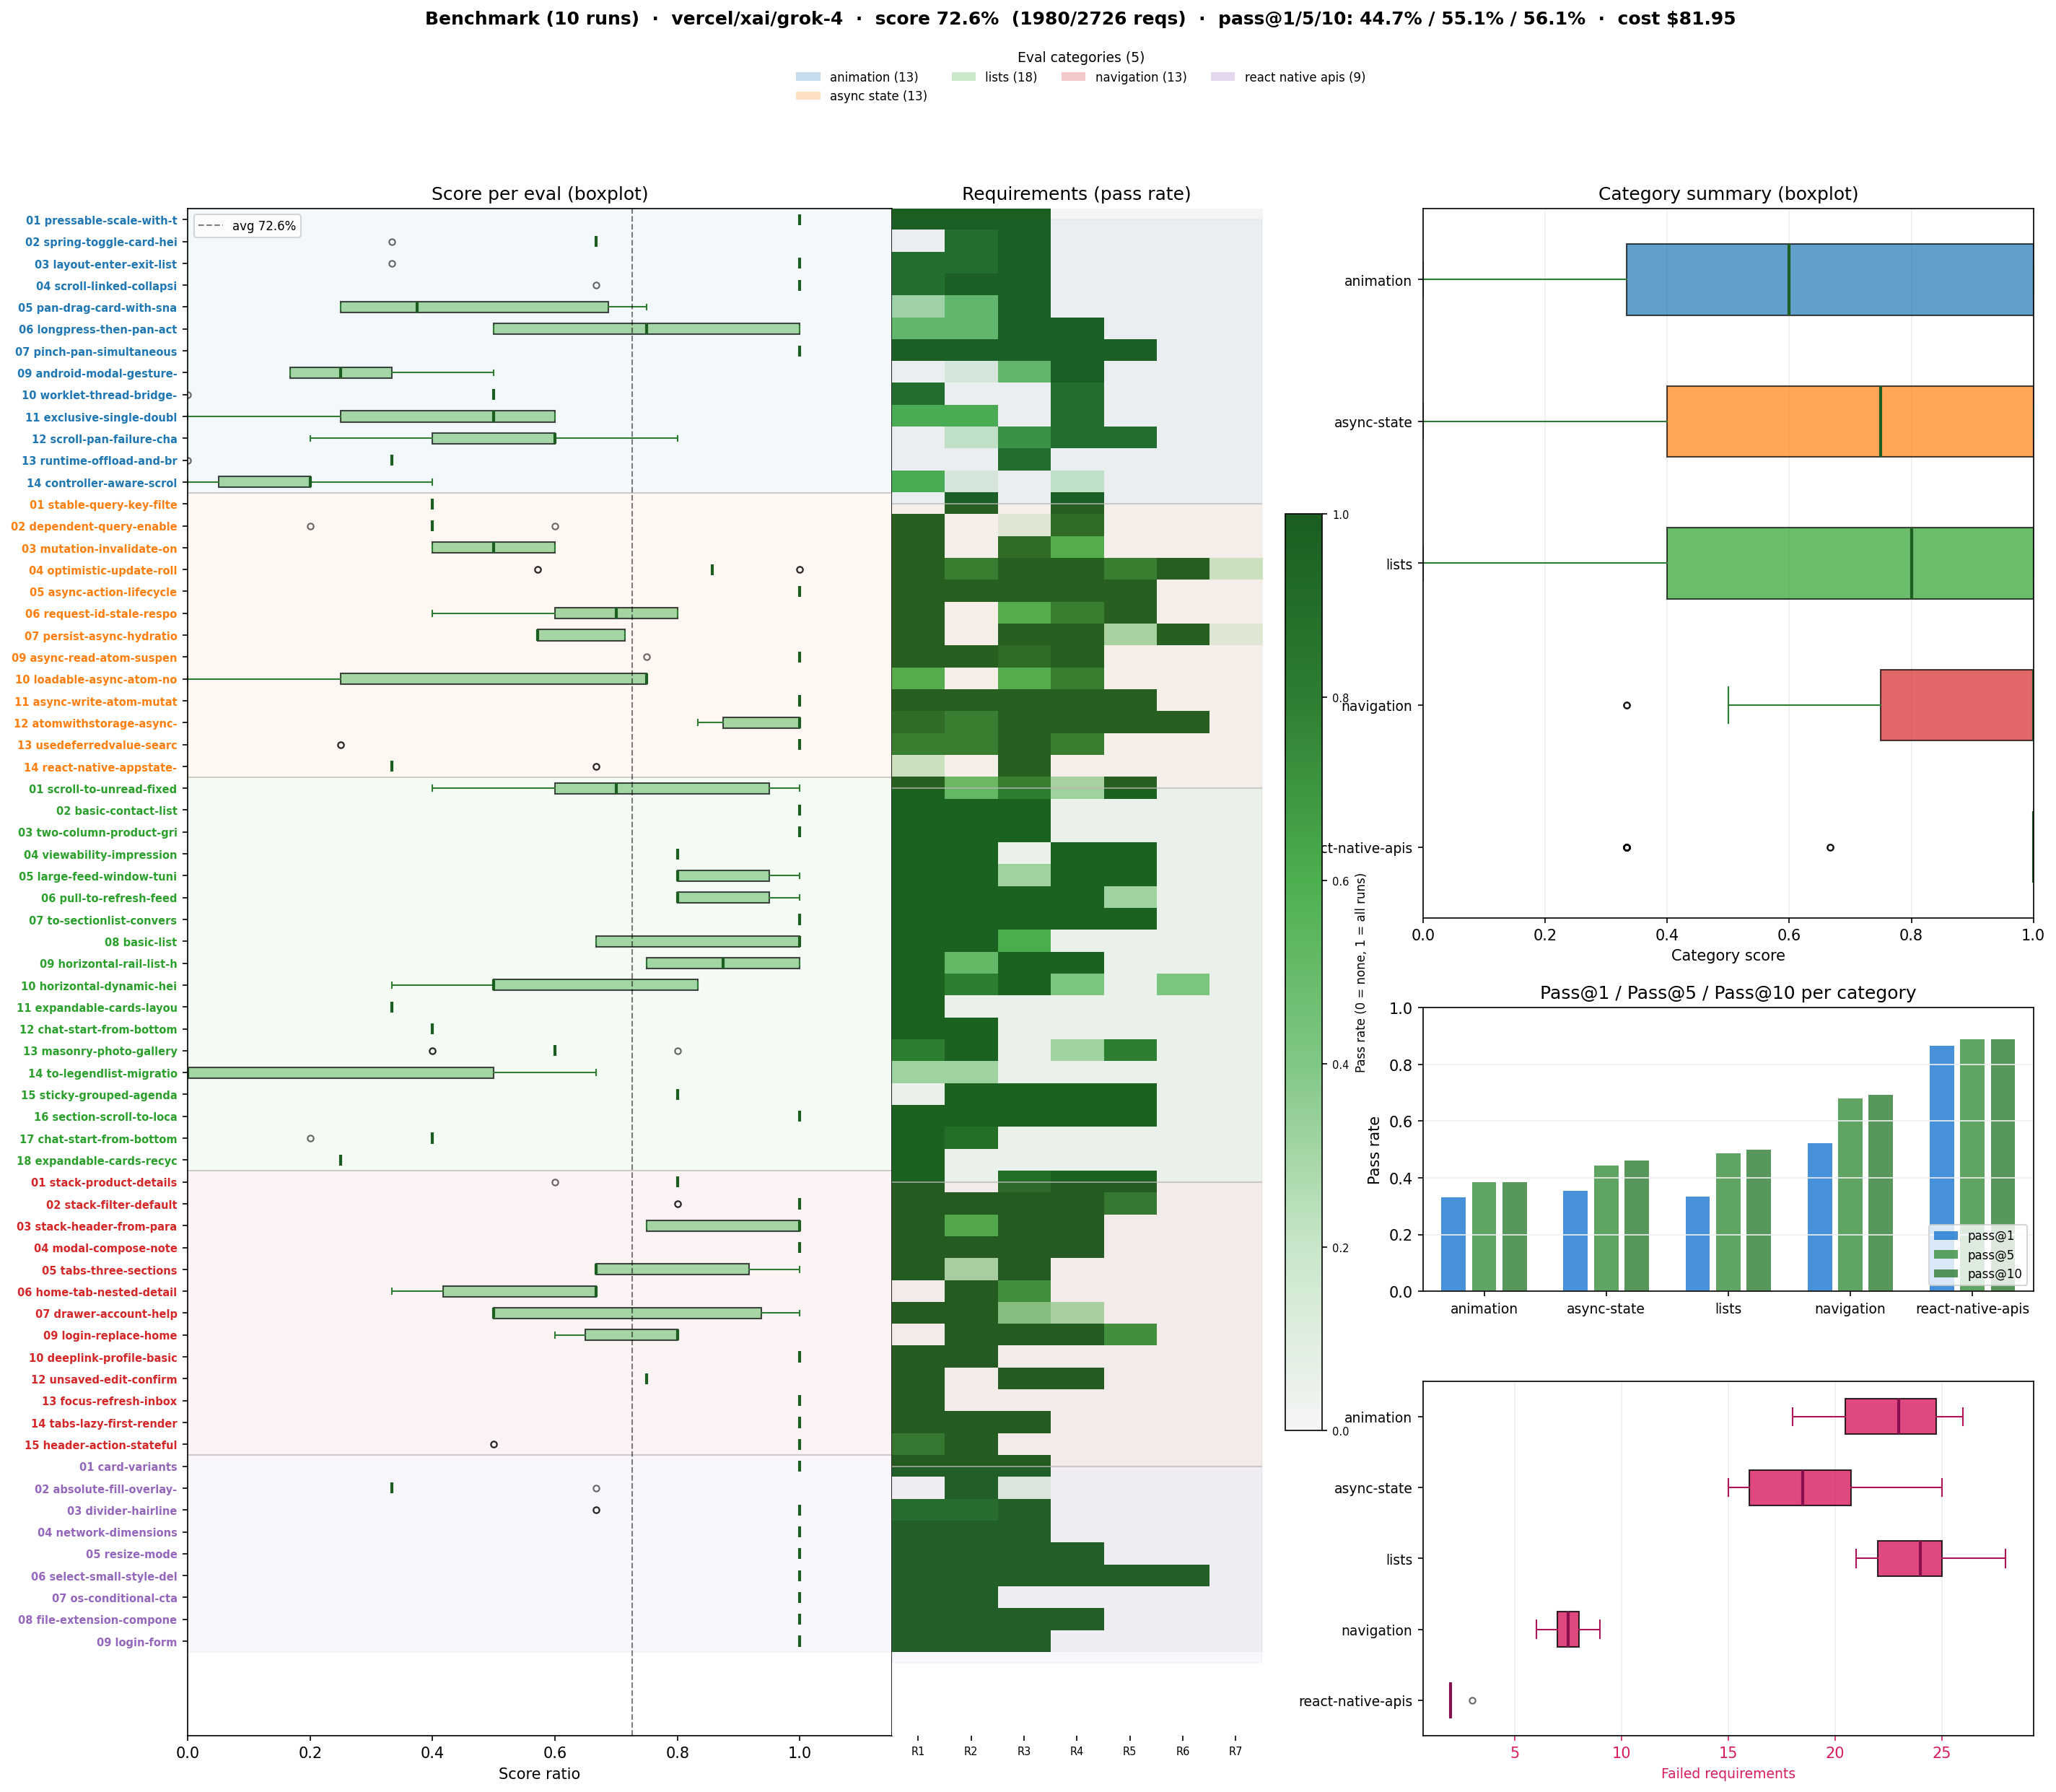
\includegraphics[width=\textwidth]{export/figures/grok-4_benchmark_plot.png}
\caption{Benchmark Plot for grok-4.}
\end{figure}

\begin{figure}[htbp]
\centering
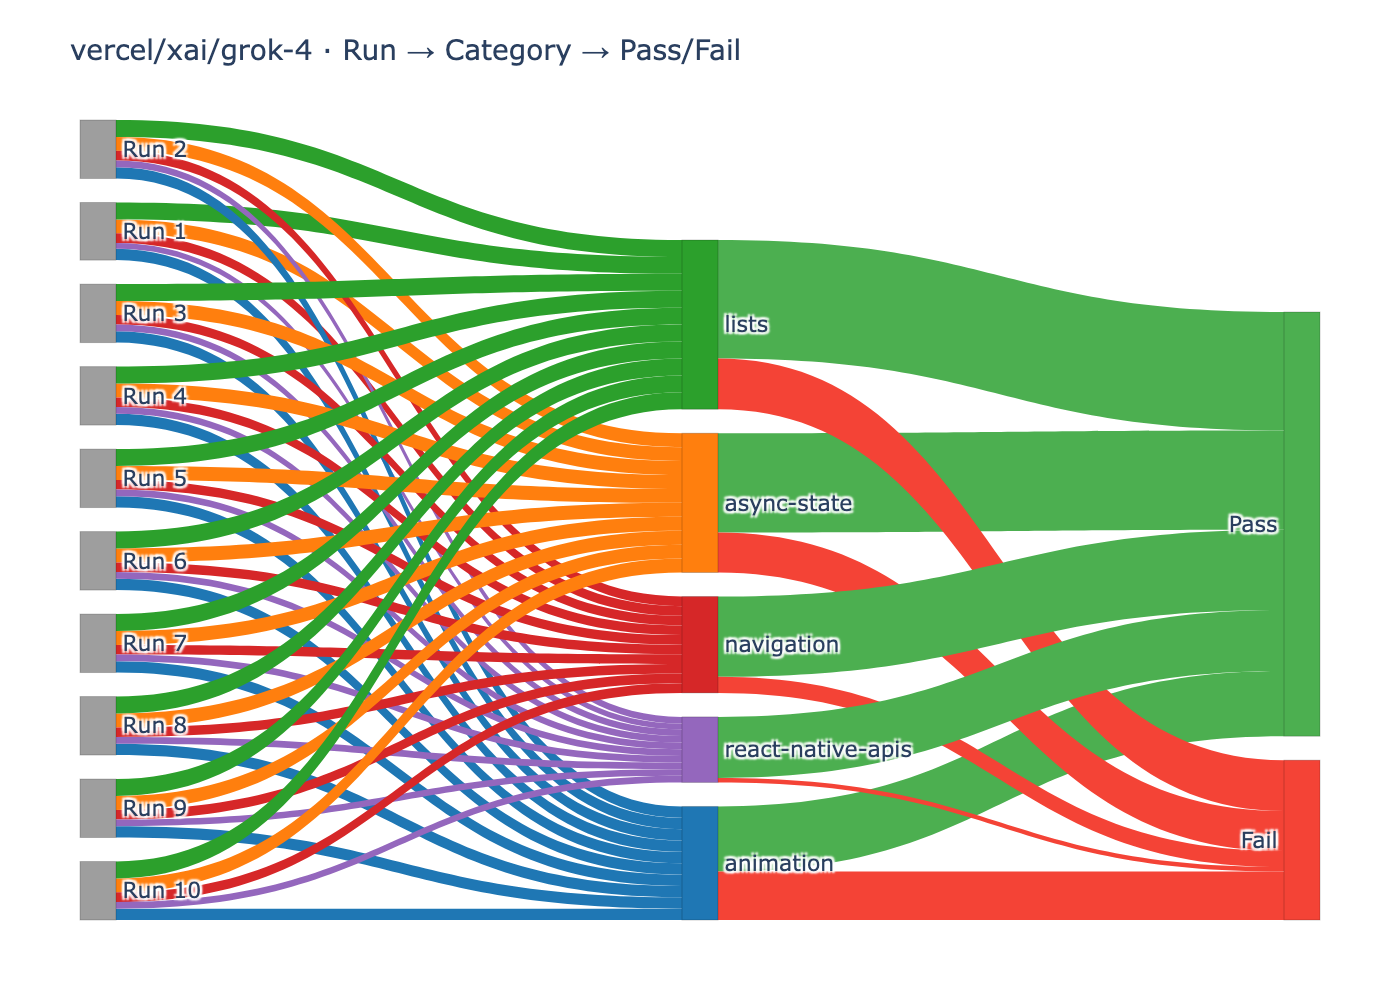
\includegraphics[width=\textwidth]{export/figures/grok-4_sankey_per_run.png}
\caption{Sankey per run for grok-4 showing the distribution of evals with respect to categories and results}
\end{figure}


\clearpage

\subsection{kimi-k2.5}

% Table: summary
% Requires: \usepackage{booktabs}
\begin{table}[htbp]
\centering
\begin{tabular}{lrrrrrr}
\toprule
Model & Runs & Score & Reqs & P@1 & P@5 & P@10 \\
\midrule
vercel/moonshotai/kimi-k2.5 & 10 & 74.9\% & 1221/1630 & 50.5\% & 66.2\% & 69.2\% \\
\bottomrule
\end{tabular}
\caption{Model summary for kimi-k2.5}
\end{table}


% Table: category_summary
% Requires: \usepackage{booktabs}
\begin{table}[htbp]
\centering
\begin{tabular}{lrrrr}
\toprule
Category & Score & Evals & Requirements & Failed requirements \\
\midrule
animation & 61.0\% & 130 & 53 & 220 \\
async state & 76.0\% & 130 & 65 & 148 \\
lists & 77.7\% & 180 & 79 & 181 \\
navigation & 91.9\% & 130 & 45 & 41 \\
react native apis & 88.3\% & 90 & 31 & 33 \\
\bottomrule
\end{tabular}
\caption{Results by category for kimi-k2.5. Score: mean(per-eval passed/total weight) across evals and runs. Evals: count of evaluation tasks. Requirements: sum of requirement count per eval. Failed requirements: sum of failed requirement instances across runs.}
\end{table}


% Table: per_eval
% Requires: \usepackage{booktabs}
\begin{table}[htbp]
\centering
\begin{adjustbox}{width=0.8\textwidth}
\begin{tabular}{lrrrrr}
\toprule
Eval & Category & Score & P@1 & P@5 & P@10 \\
\midrule
01-rn-anim-pressable-scale-with-timing & animation & 100.0\% & 100.0\% & 100.0\% & 100.0\% \\
02-rn-anim-spring-toggle-card-height & animation & 66.7\% & 30.0\% & 91.7\% & 100.0\% \\
03-rn-anim-layout-enter-exit-list-items & animation & 100.0\% & 100.0\% & 100.0\% & 100.0\% \\
04-rn-anim-scroll-linked-collapsing-header & animation & 73.3\% & 40.0\% & 97.6\% & 100.0\% \\
05-rn-anim-pan-drag-card-with-snap-points & animation & 55.0\% & 0.0\% & 0.0\% & 0.0\% \\
06-rn-anim-longpress-then-pan-activation-gate & animation & 72.5\% & 40.0\% & 97.6\% & 100.0\% \\
07-rn-anim-pinch-pan-simultaneous-photo-canvas & animation & 100.0\% & 100.0\% & 100.0\% & 100.0\% \\
09-rn-anim-android-modal-gesture-root-safety & animation & 30.0\% & 0.0\% & 0.0\% & 0.0\% \\
10-rn-anim-worklet-thread-bridge-schedule-on-rn & animation & 20.0\% & 0.0\% & 0.0\% & 0.0\% \\
11-rn-rngh-exclusive-single-double-tap & animation & 38.0\% & 0.0\% & 0.0\% & 0.0\% \\
12-rn-rngh-scroll-pan-failure-chain & animation & 70.0\% & 0.0\% & 0.0\% & 0.0\% \\
13-rn-worklets-runtime-offload-and-bridge & animation & 33.3\% & 0.0\% & 0.0\% & 0.0\% \\
14-rn-keyboard-controller-aware-scroll-footer & animation & 34.0\% & 0.0\% & 0.0\% & 0.0\% \\
01-rn-rq-stable-query-key-filters & async state & 40.0\% & 0.0\% & 0.0\% & 0.0\% \\
02-rn-rq-dependent-query-enabled-gate & async state & 46.0\% & 0.0\% & 0.0\% & 0.0\% \\
03-rn-rq-mutation-invalidate-on-success & async state & 68.0\% & 0.0\% & 0.0\% & 0.0\% \\
04-rn-rq-optimistic-update-rollback & async state & 98.6\% & 90.0\% & 100.0\% & 100.0\% \\
05-rn-zustand-async-action-lifecycle & async state & 100.0\% & 100.0\% & 100.0\% & 100.0\% \\
06-rn-zustand-request-id-stale-response-guard & async state & 68.0\% & 20.0\% & 77.8\% & 100.0\% \\
07-rn-zustand-persist-async-hydration-gate & async state & 72.9\% & 30.0\% & 91.7\% & 100.0\% \\
09-rn-jotai-async-read-atom-suspense & async state & 97.5\% & 90.0\% & 100.0\% & 100.0\% \\
10-rn-jotai-loadable-async-atom-no-suspense & async state & 50.0\% & 0.0\% & 0.0\% & 0.0\% \\
11-rn-jotai-async-write-atom-mutation & async state & 100.0\% & 100.0\% & 100.0\% & 100.0\% \\
12-rn-jotai-atomwithstorage-async-rehydrate-guard & async state & 93.3\% & 60.0\% & 100.0\% & 100.0\% \\
13-rn-react-usedeferredvalue-search-stale-indicator & async state & 100.0\% & 100.0\% & 100.0\% & 100.0\% \\
14-rn-rq-react-native-appstate-focus-online-managers & async state & 53.3\% & 0.0\% & 0.0\% & 0.0\% \\
01-rn-flatlist-scroll-to-unread-fixed-rows & lists & 90.0\% & 70.0\% & 100.0\% & 100.0\% \\
02-rn-flatlist-basic-contact-list & lists & 100.0\% & 100.0\% & 100.0\% & 100.0\% \\
03-rn-flatlist-two-column-product-grid & lists & 100.0\% & 100.0\% & 100.0\% & 100.0\% \\
04-rn-flatlist-viewability-impression-tracking & lists & 80.0\% & 0.0\% & 0.0\% & 0.0\% \\
05-rn-flatlist-large-feed-window-tuning & lists & 86.0\% & 30.0\% & 91.7\% & 100.0\% \\
06-rn-flatlist-pull-to-refresh-feed & lists & 84.0\% & 20.0\% & 77.8\% & 100.0\% \\
07-rn-flatlist-to-sectionlist-conversion & lists & 86.0\% & 30.0\% & 91.7\% & 100.0\% \\
08-rn-flashlist-basic-list & lists & 100.0\% & 100.0\% & 100.0\% & 100.0\% \\
09-rn-flashlist-horizontal-rail-list-header & lists & 80.0\% & 20.0\% & 77.8\% & 100.0\% \\
10-rn-flashlist-horizontal-dynamic-height-header-first-item & lists & 83.3\% & 0.0\% & 0.0\% & 0.0\% \\
11-rn-flashlist-expandable-cards-layout-state & lists & 60.0\% & 0.0\% & 0.0\% & 0.0\% \\
12-rn-flashlist-chat-start-from-bottom & lists & 54.0\% & 0.0\% & 0.0\% & 0.0\% \\
13-rn-flashlist-masonry-photo-gallery & lists & 60.0\% & 0.0\% & 0.0\% & 0.0\% \\
14-rn-flatlist-to-legendlist-migration & lists & 70.0\% & 10.0\% & 50.0\% & 100.0\% \\
15-rn-legendlist-sticky-grouped-agenda & lists & 82.0\% & 20.0\% & 77.8\% & 100.0\% \\
16-rn-legendlist-section-scroll-to-location & lists & 100.0\% & 100.0\% & 100.0\% & 100.0\% \\
17-rn-legendlist-chat-start-from-bottom & lists & 40.0\% & 0.0\% & 0.0\% & 0.0\% \\
18-rn-legendlist-expandable-cards-recycling-state & lists & 42.5\% & 0.0\% & 0.0\% & 0.0\% \\
01-rn-nav-stack-product-details & navigation & 78.0\% & 20.0\% & 77.8\% & 100.0\% \\
02-rn-nav-stack-filter-default & navigation & 100.0\% & 100.0\% & 100.0\% & 100.0\% \\
03-rn-nav-stack-header-from-param & navigation & 87.5\% & 50.0\% & 99.6\% & 100.0\% \\
04-rn-nav-modal-compose-note & navigation & 100.0\% & 100.0\% & 100.0\% & 100.0\% \\
05-rn-nav-tabs-three-sections & navigation & 100.0\% & 100.0\% & 100.0\% & 100.0\% \\
06-rn-nav-home-tab-nested-details & navigation & 86.7\% & 60.0\% & 100.0\% & 100.0\% \\
07-rn-nav-drawer-account-help & navigation & 100.0\% & 100.0\% & 100.0\% & 100.0\% \\
09-rn-nav-login-replace-home & navigation & 72.0\% & 10.0\% & 50.0\% & 100.0\% \\
10-rn-nav-deeplink-profile-basic & navigation & 95.0\% & 90.0\% & 100.0\% & 100.0\% \\
12-rn-nav-unsaved-edit-confirm & navigation & 95.0\% & 80.0\% & 100.0\% & 100.0\% \\
13-rn-nav-focus-refresh-inbox & navigation & 100.0\% & 100.0\% & 100.0\% & 100.0\% \\
14-rn-nav-tabs-lazy-first-render & navigation & 100.0\% & 100.0\% & 100.0\% & 100.0\% \\
15-rn-nav-header-action-stateful & navigation & 80.0\% & 60.0\% & 100.0\% & 100.0\% \\
01-rn-stylesheet-card-variants & react native apis & 100.0\% & 100.0\% & 100.0\% & 100.0\% \\
02-rn-stylesheet-absolute-fill-overlay-badge & react native apis & 40.0\% & 0.0\% & 0.0\% & 0.0\% \\
03-rn-stylesheet-divider-hairline & react native apis & 70.0\% & 20.0\% & 77.8\% & 100.0\% \\
04-rn-image-network-dimensions & react native apis & 100.0\% & 100.0\% & 100.0\% & 100.0\% \\
05-rn-imagebackground-resize-mode & react native apis & 85.0\% & 70.0\% & 100.0\% & 100.0\% \\
06-rn-platform-select-small-style-delta & react native apis & 100.0\% & 100.0\% & 100.0\% & 100.0\% \\
07-rn-platform-os-conditional-cta & react native apis & 100.0\% & 100.0\% & 100.0\% & 100.0\% \\
08-rn-platform-file-extension-component-split & react native apis & 100.0\% & 100.0\% & 100.0\% & 100.0\% \\
09-rn-keyboardavoidingview-login-form & react native apis & 100.0\% & 100.0\% & 100.0\% & 100.0\% \\
\bottomrule
\end{tabular}
\end{adjustbox}
\caption{Per-eval results (score and pass@k) for kimi-k2.5}
\end{table}


\begin{figure}[htbp]
\centering
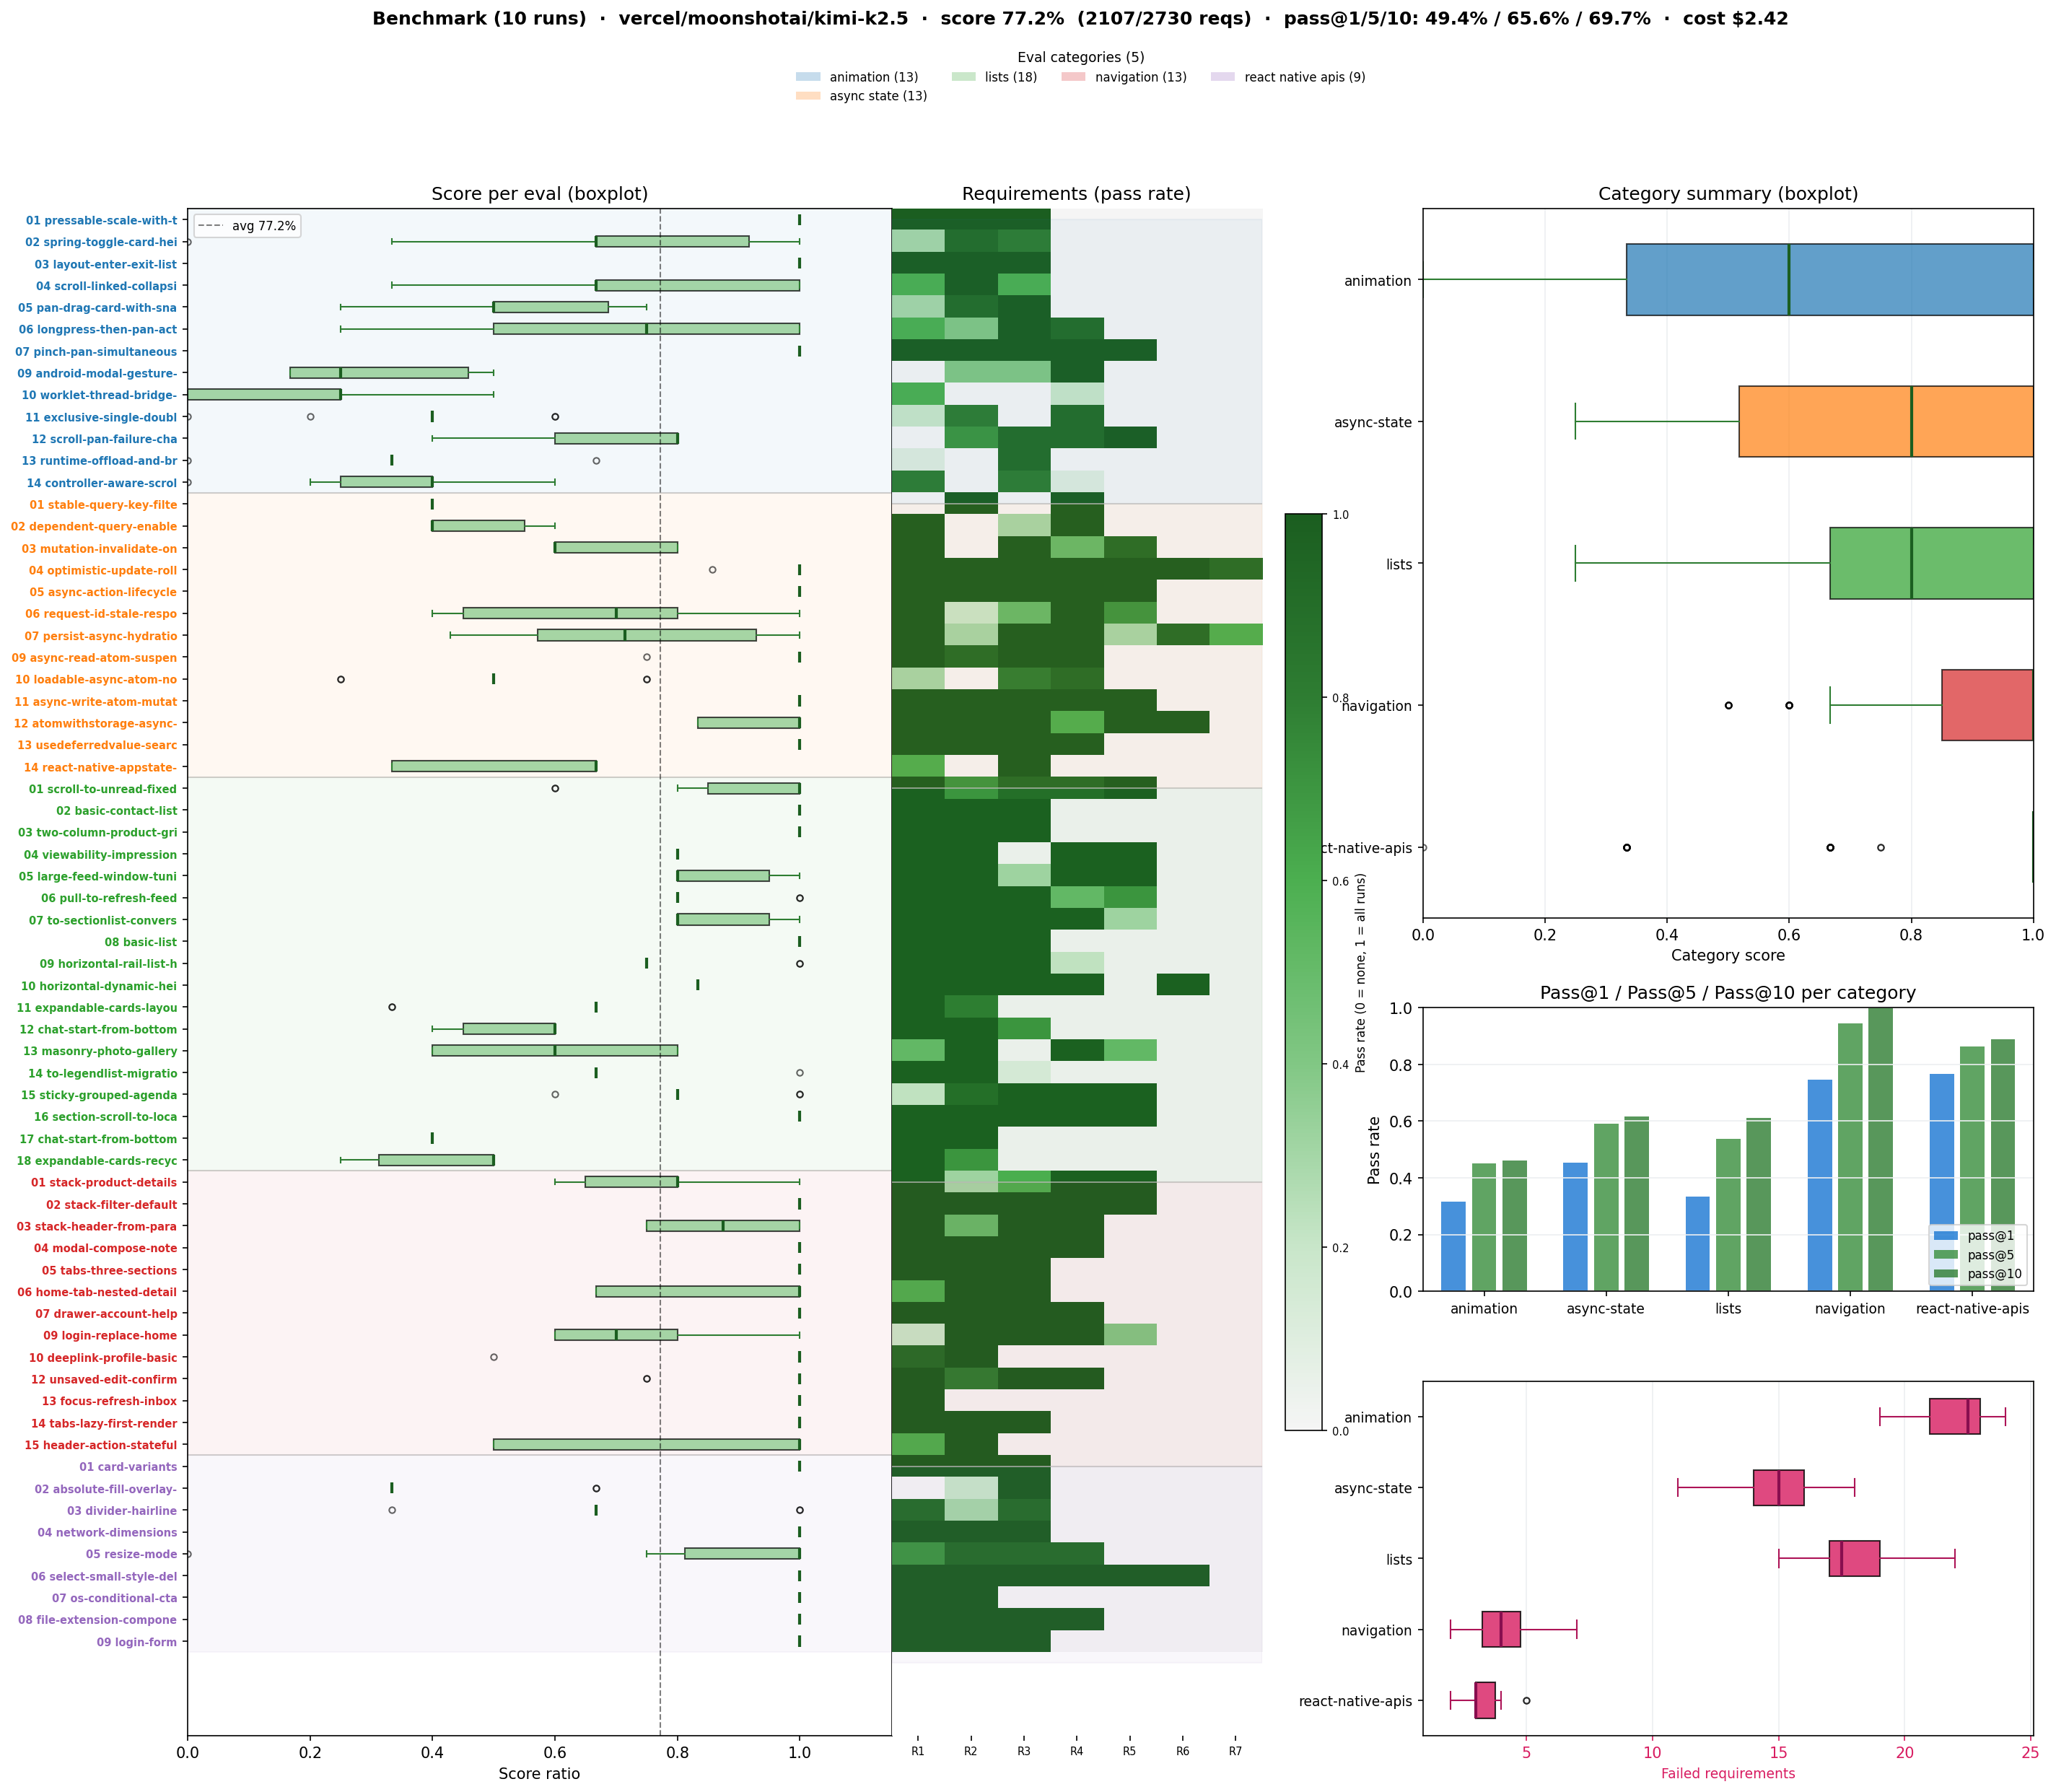
\includegraphics[width=\textwidth]{export/figures/kimi-k2.5_benchmark_plot.png}
\caption{Benchmark Plot for kimi-k2.5.}
\end{figure}

\begin{figure}[htbp]
\centering
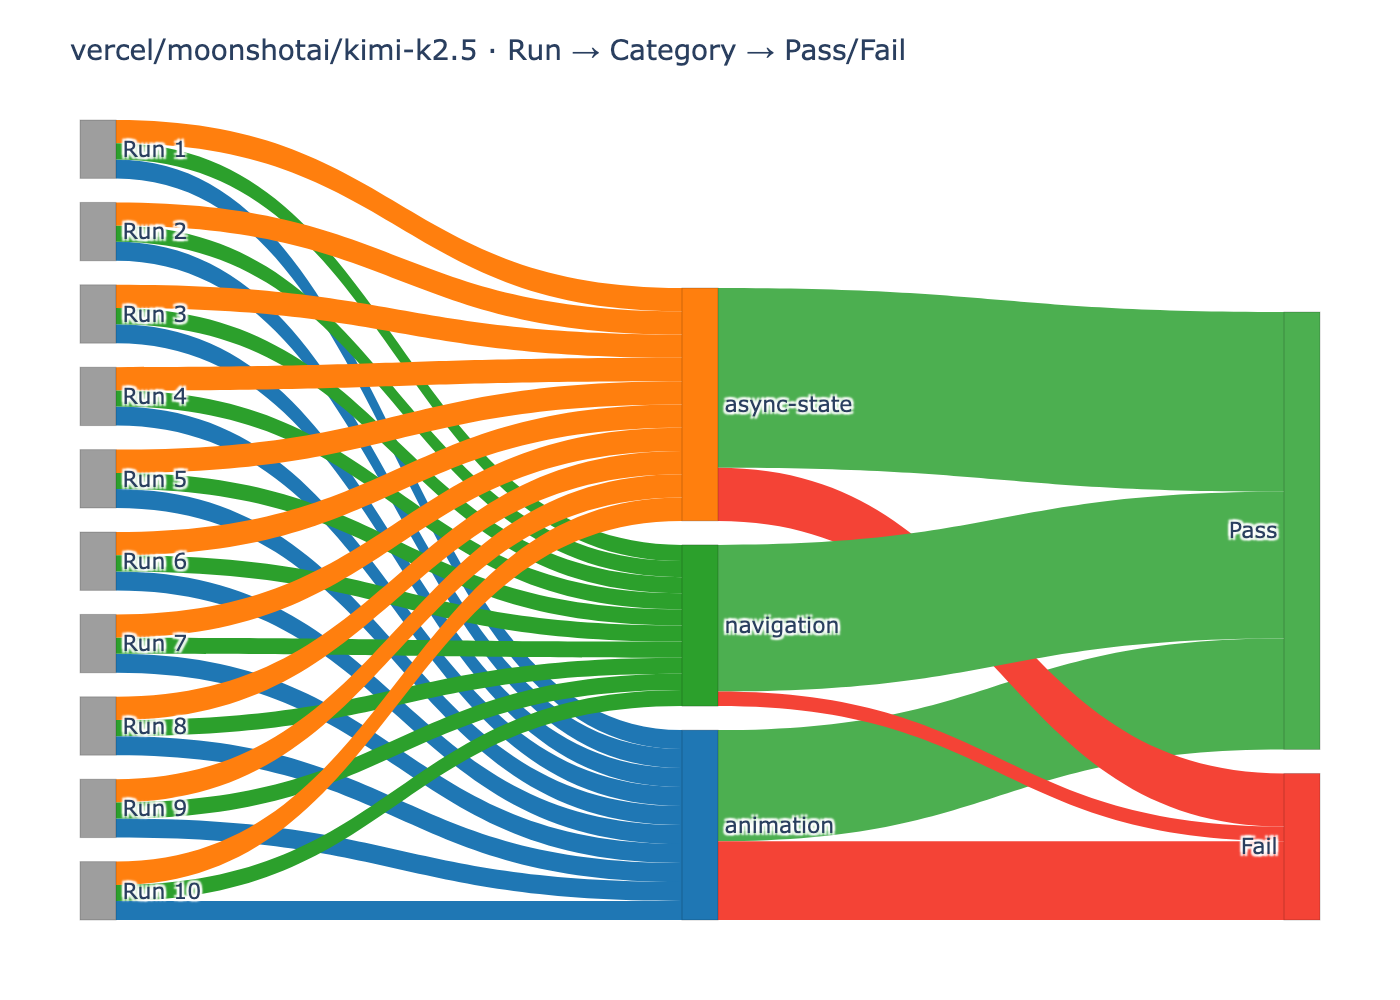
\includegraphics[width=\textwidth]{export/figures/kimi-k2.5_sankey_per_run.png}
\caption{Sankey per run for kimi-k2.5 showing the distribution of evals with respect to categories and results}
\end{figure}


\clearpage

\subsection{qwen2.5-coder-32b-instruct}

% Table: summary
% Requires: \usepackage{booktabs}
\begin{table}[htbp]
\centering
\begin{tabular}{lrrrrrr}
\toprule
Model & Runs & Score & Reqs & P@1 & P@5 & P@10 \\
\midrule
cloudflare-ai-gateway/workers-ai/@cf/qwen/qwen2.5- & 10 & 51.2\% & 1316/2570 & 18.8\% & 29.3\% & 28.8\% \\
\bottomrule
\end{tabular}
\caption{Model summary for qwen2.5-coder-32b-instruct}
\end{table}


% Table: category_summary
% Requires: \usepackage{booktabs}
\begin{table}[htbp]
\centering
\begin{tabular}{lrrrr}
\toprule
Category & Score & Evals & Requirements & Failed requirements \\
\midrule
animation & 25.9\% & 122 & 53 & 389 \\
async state & 44.4\% & 121 & 65 & 329 \\
lists & 57.3\% & 176 & 79 & 318 \\
navigation & 66.1\% & 111 & 45 & 140 \\
react native apis & 70.2\% & 86 & 31 & 78 \\
\bottomrule
\end{tabular}
\caption{Results by category for qwen2.5-coder-32b-instruct. Score: mean(per-eval passed/total weight) across evals and runs. Evals: count of evaluation tasks. Requirements: sum of requirement count per eval. Failed requirements: sum of failed requirement instances across runs.}
\end{table}


% Table: per_eval
% Requires: \usepackage{booktabs}
\begin{table}[htbp]
\centering
\begin{tabular}{lrrrrr}
\toprule
Eval & Category & Score & P@1 & P@5 & P@10 \\
\midrule
01-rn-anim-pressable-scale-with-timing & animation & 53.3\% & 0.0\% & 0.0\% & 0.0\% \\
02-rn-anim-spring-toggle-card-height & animation & 40.7\% & 0.0\% & 0.0\% & 0.0\% \\
03-rn-anim-layout-enter-exit-list-items & animation & 90.0\% & 80.0\% & 100.0\% & 100.0\% \\
04-rn-anim-scroll-linked-collapsing-header & animation & 46.7\% & 20.0\% & 77.8\% & 100.0\% \\
05-rn-anim-pan-drag-card-with-snap-points & animation & 10.0\% & 0.0\% & 0.0\% & 0.0\% \\
06-rn-anim-longpress-then-pan-activation-gate & animation & 22.5\% & 0.0\% & 0.0\% & 0.0\% \\
07-rn-anim-pinch-pan-simultaneous-photo-canvas & animation & 48.0\% & 0.0\% & 0.0\% & 0.0\% \\
09-rn-anim-android-modal-gesture-root-safety & animation & 3.7\% & 0.0\% & 0.0\% & 0.0\% \\
10-rn-anim-worklet-thread-bridge-schedule-on-rn & animation & 17.5\% & 0.0\% & 0.0\% & 0.0\% \\
11-rn-rngh-exclusive-single-double-tap & animation & 2.0\% & 0.0\% & 0.0\% & 0.0\% \\
12-rn-rngh-scroll-pan-failure-chain & animation & 4.4\% & 0.0\% & 0.0\% & 0.0\% \\
13-rn-worklets-runtime-offload-and-bridge & animation & 6.7\% & 0.0\% & 0.0\% & 0.0\% \\
14-rn-keyboard-controller-aware-scroll-footer & animation & 2.0\% & 0.0\% & 0.0\% & 0.0\% \\
01-rn-rq-stable-query-key-filters & async state & 10.0\% & 0.0\% & 0.0\% & 0.0\% \\
02-rn-rq-dependent-query-enabled-gate & async state & 18.0\% & 0.0\% & 0.0\% & 0.0\% \\
03-rn-rq-mutation-invalidate-on-success & async state & 22.0\% & 0.0\% & 0.0\% & 0.0\% \\
04-rn-rq-optimistic-update-rollback & async state & 62.9\% & 0.0\% & 0.0\% & 0.0\% \\
05-rn-zustand-async-action-lifecycle & async state & 92.0\% & 60.0\% & 100.0\% & 100.0\% \\
06-rn-zustand-request-id-stale-response-guard & async state & 22.0\% & 0.0\% & 0.0\% & 0.0\% \\
07-rn-zustand-persist-async-hydration-gate & async state & 41.4\% & 0.0\% & 0.0\% & 0.0\% \\
09-rn-jotai-async-read-atom-suspense & async state & 22.5\% & 0.0\% & 0.0\% & 0.0\% \\
10-rn-jotai-loadable-async-atom-no-suspense & async state & 12.5\% & 0.0\% & 0.0\% & 0.0\% \\
11-rn-jotai-async-write-atom-mutation & async state & 66.0\% & 0.0\% & 0.0\% & 0.0\% \\
12-rn-jotai-atomwithstorage-async-rehydrate-guard & async state & 60.0\% & 0.0\% & 0.0\% & 0.0\% \\
13-rn-react-usedeferredvalue-search-stale-indicator & async state & 91.7\% & 66.7\% & 100.0\% & 66.7\% \\
14-rn-rq-react-native-appstate-focus-online-managers & async state & 33.3\% & 0.0\% & 0.0\% & 0.0\% \\
01-rn-nav-stack-product-details & navigation & 60.0\% & 0.0\% & 0.0\% & 0.0\% \\
02-rn-nav-stack-filter-default & navigation & 94.0\% & 80.0\% & 100.0\% & 100.0\% \\
03-rn-nav-stack-header-from-param & navigation & 56.2\% & 12.5\% & 62.5\% & 12.5\% \\
04-rn-nav-modal-compose-note & navigation & 75.0\% & 0.0\% & 0.0\% & 0.0\% \\
05-rn-nav-tabs-three-sections & navigation & 73.3\% & 20.0\% & 100.0\% & 20.0\% \\
06-rn-nav-home-tab-nested-details & navigation & 43.3\% & 10.0\% & 50.0\% & 100.0\% \\
07-rn-nav-drawer-account-help & navigation & 50.0\% & 0.0\% & 0.0\% & 0.0\% \\
09-rn-nav-login-replace-home & navigation & 42.0\% & 0.0\% & 0.0\% & 0.0\% \\
10-rn-nav-deeplink-profile-basic & navigation & 100.0\% & 100.0\% & 100.0\% & 100.0\% \\
12-rn-nav-unsaved-edit-confirm & navigation & 55.0\% & 0.0\% & 0.0\% & 0.0\% \\
13-rn-nav-focus-refresh-inbox & navigation & 100.0\% & 100.0\% & 100.0\% & 100.0\% \\
14-rn-nav-tabs-lazy-first-render & navigation & 66.7\% & 0.0\% & 0.0\% & 0.0\% \\
15-rn-nav-header-action-stateful & navigation & 44.4\% & 0.0\% & 0.0\% & 0.0\% \\
\bottomrule
\end{tabular}
\caption{Per-eval results (score and pass@k) for qwen2.5-coder-32b-instruct}
\end{table}


\begin{figure}[htbp]
\centering
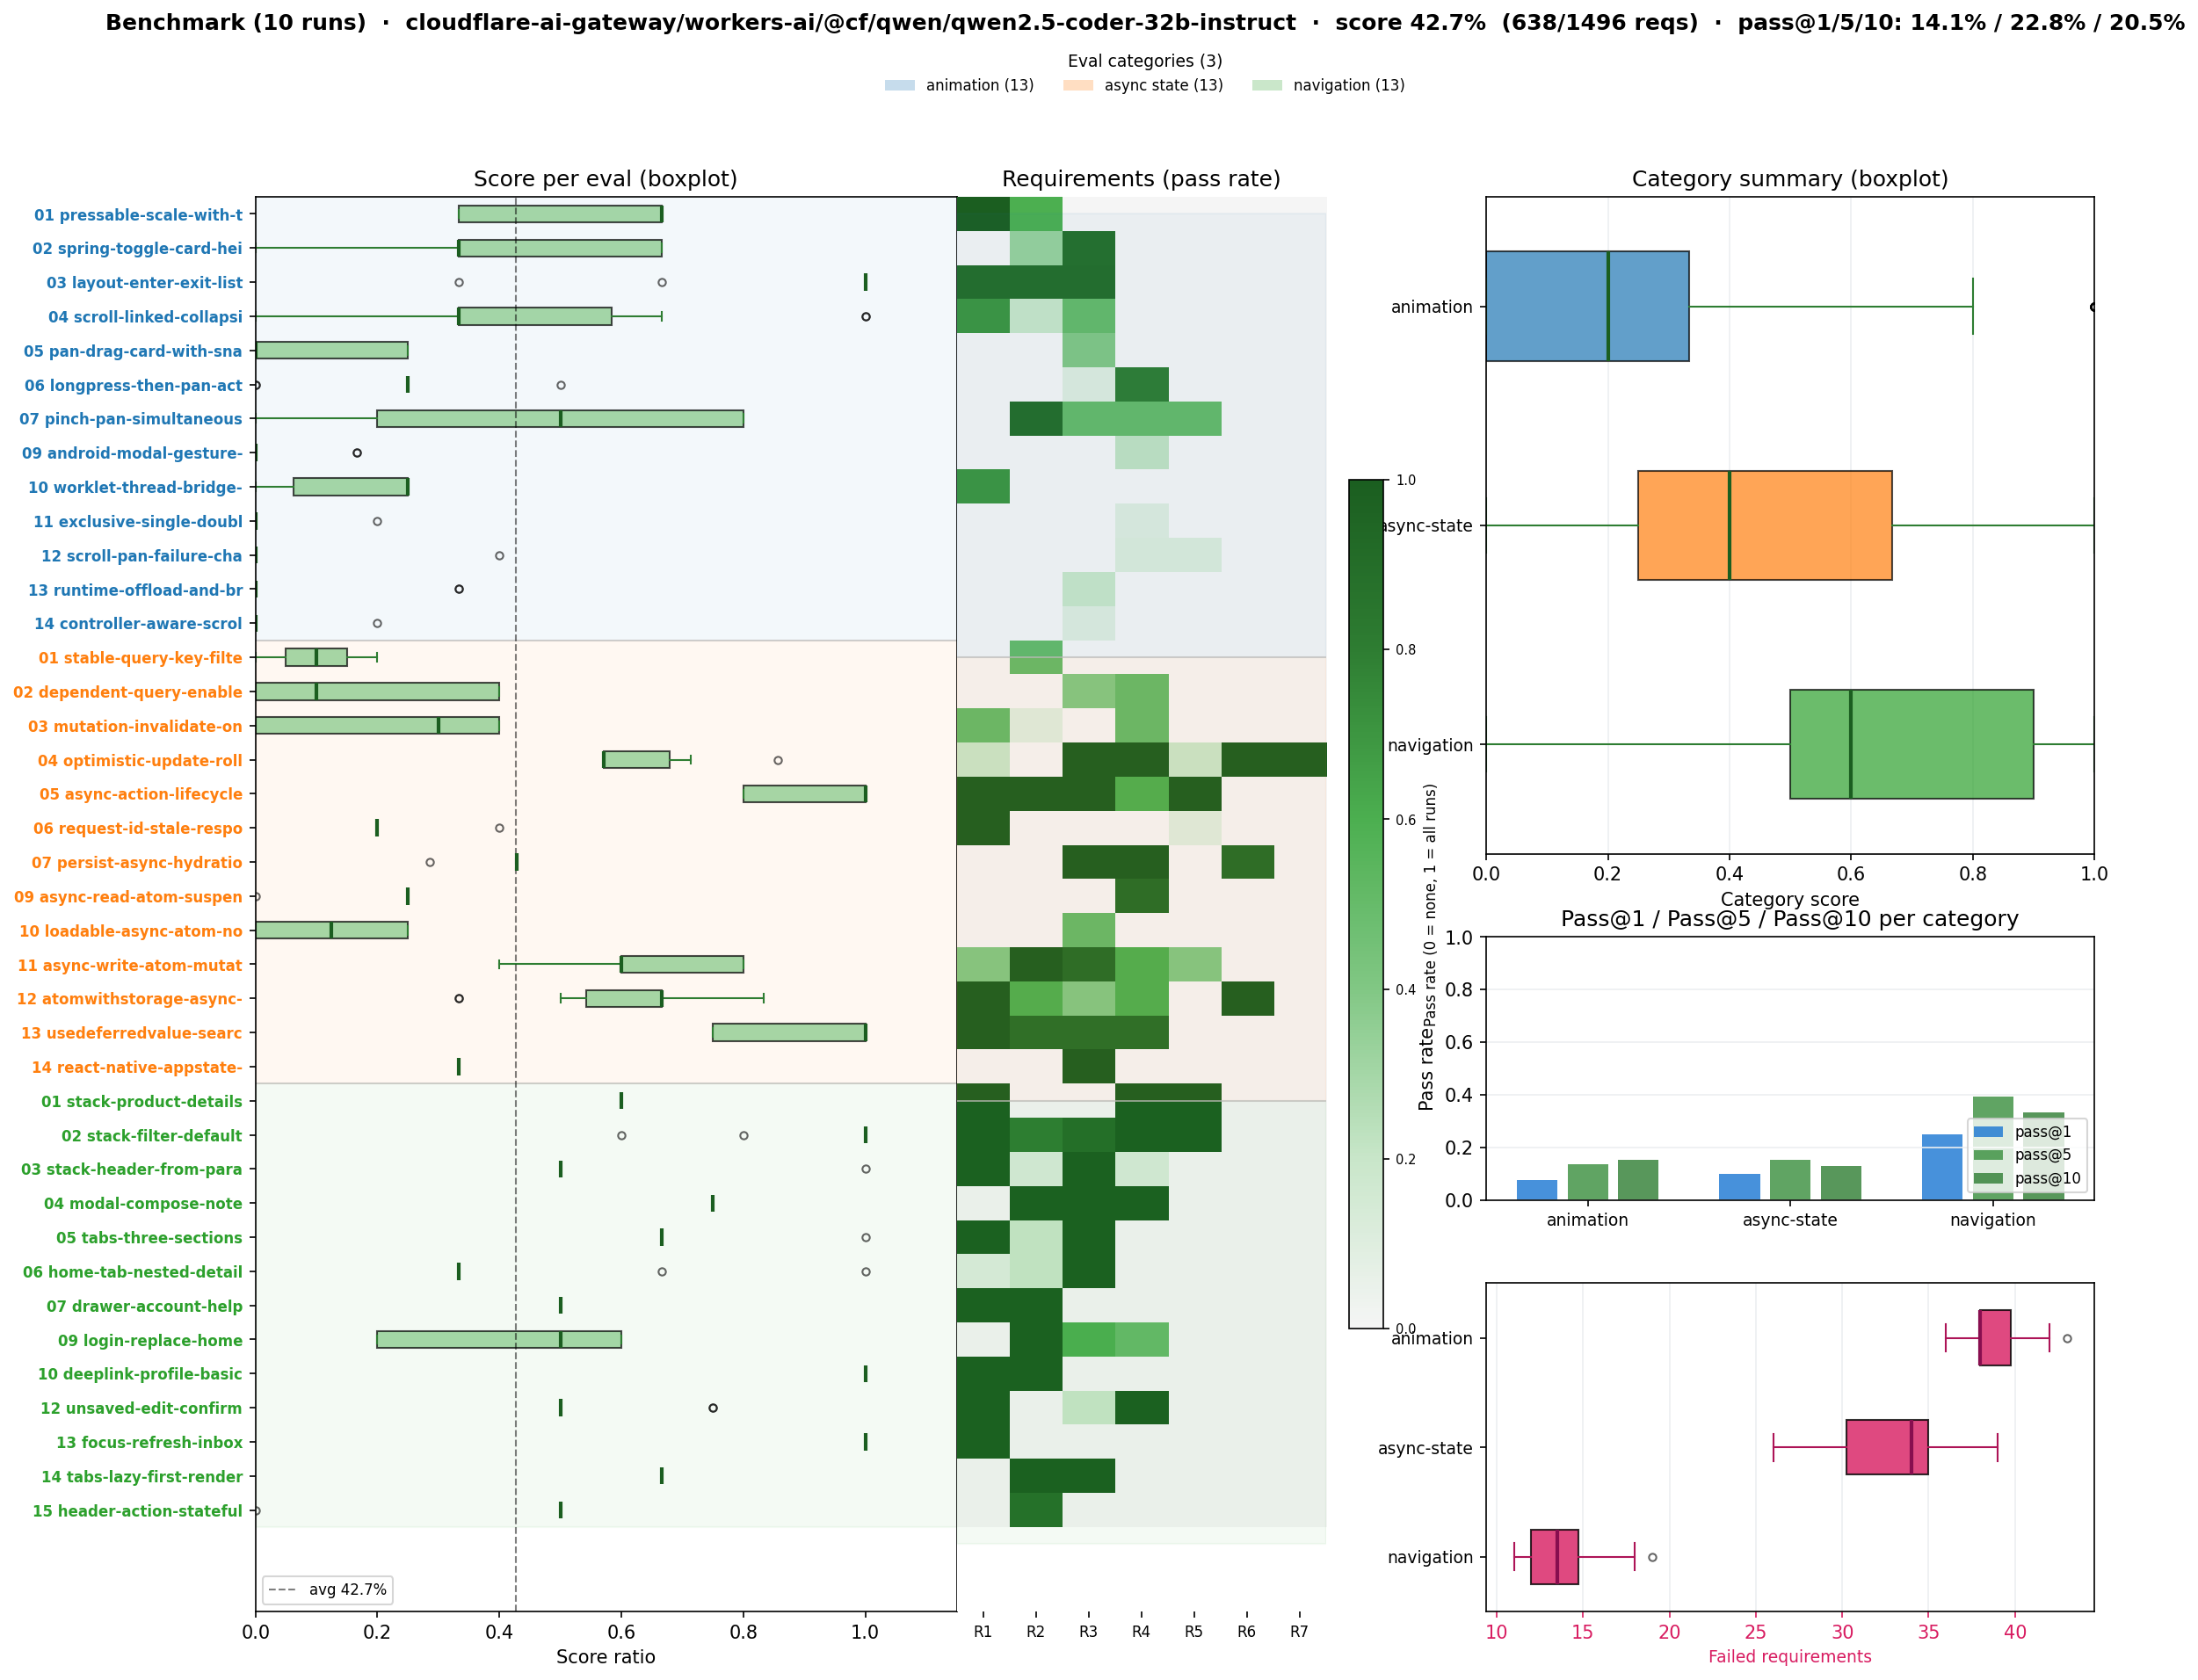
\includegraphics[width=\textwidth]{export/figures/qwen2.5-coder-32b-instruct_benchmark_plot.png}
\caption{Benchmark Plot for qwen2.5-coder-32b-instruct.}
\end{figure}

\begin{figure}[htbp]
\centering
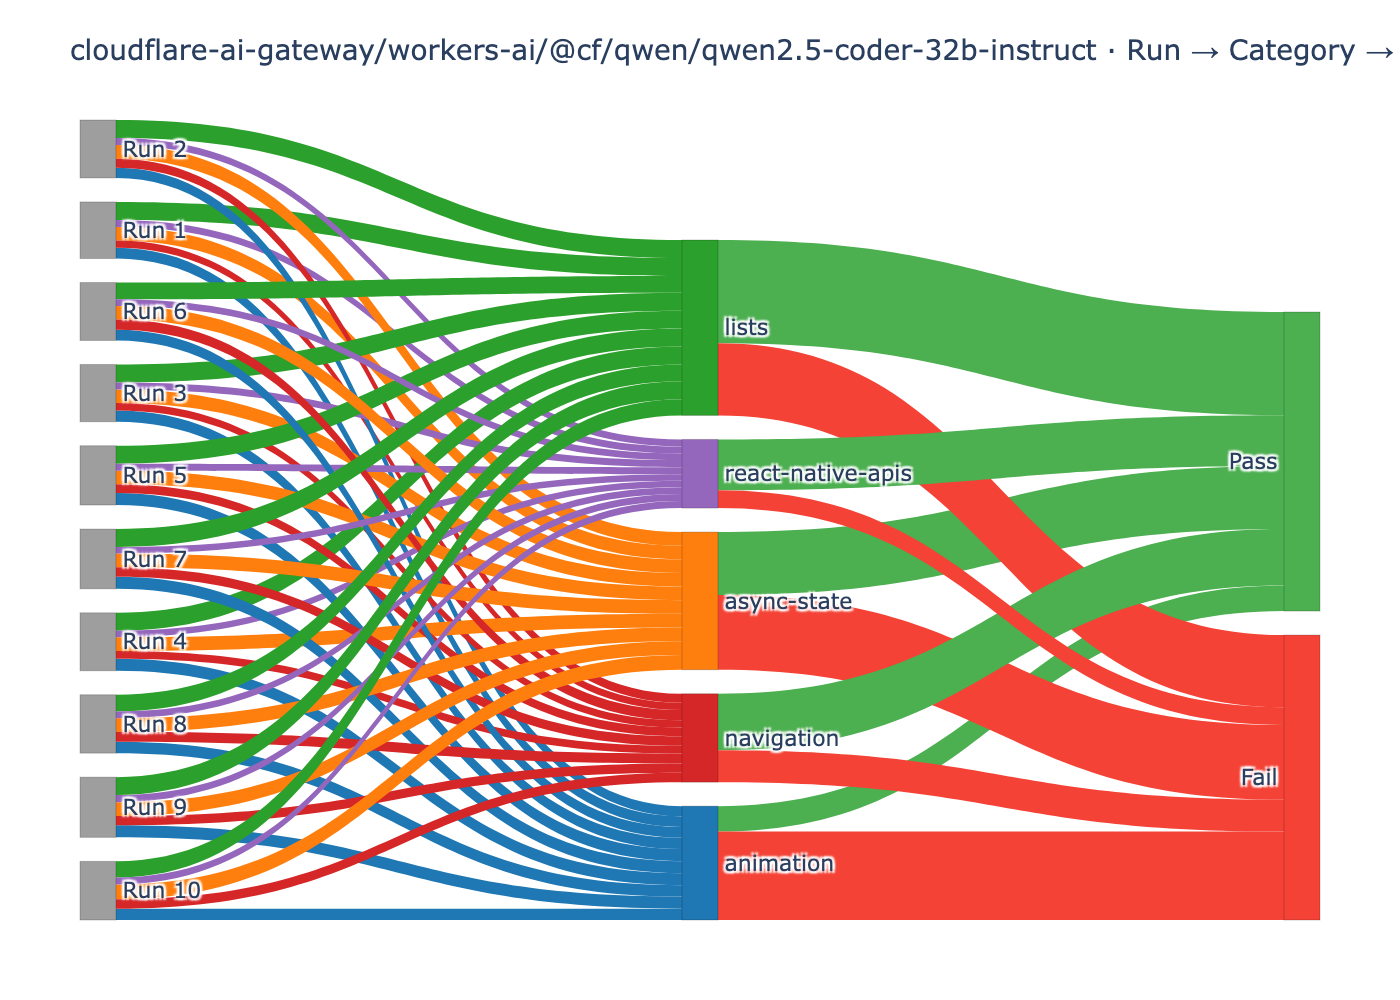
\includegraphics[width=\textwidth]{export/figures/qwen2.5-coder-32b-instruct_sankey_per_run.png}
\caption{Sankey per run for qwen2.5-coder-32b-instruct showing the distribution of evals with respect to categories and results}
\end{figure}
 (compile from repo root)

\appendix
\section{Detailed Results}

\subsection{claude-opus-4.6}

% Table: summary
% Requires: \usepackage{booktabs}
\begin{table}[htbp]
\centering
\begin{tabular}{lrrrrrr}
\toprule
Model & Runs & Score & Reqs & P@1 & P@5 & P@10 \\
\midrule
vercel/anthropic/claude-opus-4.6 & 10 & 84.1\% & 2296/2730 & 60.6\% & 66.8\% & 69.7\% \\
\bottomrule
\end{tabular}
\caption{Model summary for claude-opus-4.6}
\end{table}


% Table: category_summary
% Requires: \usepackage{booktabs}
\begin{table}[htbp]
\centering
\begin{tabular}{lrrrr}
\toprule
Category & Score & Evals & Requirements & Failed requirements \\
\midrule
animation & 77.8\% & 130 & 53 & 121 \\
async state & 83.6\% & 130 & 65 & 106 \\
navigation & 94.5\% & 130 & 45 & 28 \\
\bottomrule
\end{tabular}
\caption{Results by category for claude-opus-4.6. Score: mean(per-eval passed/total weight) across evals and runs. Evals: count of evaluation tasks. Requirements: sum of requirement count per eval. Failed requirements: sum of failed requirement instances across runs.}
\end{table}


% Table: per_eval
% Requires: \usepackage{booktabs}
\begin{table}[htbp]
\centering
\begin{tabular}{lrrrrr}
\toprule
Eval & Category & Score & P@1 & P@5 & P@10 \\
\midrule
01-rn-anim-pressable-scale-with-timing & animation & 100.0\% & 100.0\% & 100.0\% & 100.0\% \\
02-rn-anim-spring-toggle-card-height & animation & 83.3\% & 50.0\% & 99.6\% & 100.0\% \\
03-rn-anim-layout-enter-exit-list-items & animation & 100.0\% & 100.0\% & 100.0\% & 100.0\% \\
04-rn-anim-scroll-linked-collapsing-header & animation & 100.0\% & 100.0\% & 100.0\% & 100.0\% \\
05-rn-anim-pan-drag-card-with-snap-points & animation & 77.5\% & 10.0\% & 50.0\% & 100.0\% \\
06-rn-anim-longpress-then-pan-activation-gate & animation & 100.0\% & 100.0\% & 100.0\% & 100.0\% \\
07-rn-anim-pinch-pan-simultaneous-photo-canvas & animation & 100.0\% & 100.0\% & 100.0\% & 100.0\% \\
09-rn-anim-android-modal-gesture-root-safety & animation & 83.3\% & 0.0\% & 0.0\% & 0.0\% \\
10-rn-anim-worklet-thread-bridge-schedule-on-rn & animation & 37.5\% & 0.0\% & 0.0\% & 0.0\% \\
11-rn-rngh-exclusive-single-double-tap & animation & 62.0\% & 0.0\% & 0.0\% & 0.0\% \\
12-rn-rngh-scroll-pan-failure-chain & animation & 80.0\% & 0.0\% & 0.0\% & 0.0\% \\
13-rn-worklets-runtime-offload-and-bridge & animation & 33.3\% & 0.0\% & 0.0\% & 0.0\% \\
14-rn-keyboard-controller-aware-scroll-footer & animation & 54.0\% & 0.0\% & 0.0\% & 0.0\% \\
01-rn-rq-stable-query-key-filters & async state & 56.0\% & 0.0\% & 0.0\% & 0.0\% \\
02-rn-rq-dependent-query-enabled-gate & async state & 58.0\% & 0.0\% & 0.0\% & 0.0\% \\
03-rn-rq-mutation-invalidate-on-success & async state & 44.0\% & 0.0\% & 0.0\% & 0.0\% \\
04-rn-rq-optimistic-update-rollback & async state & 95.7\% & 70.0\% & 100.0\% & 100.0\% \\
05-rn-zustand-async-action-lifecycle & async state & 100.0\% & 100.0\% & 100.0\% & 100.0\% \\
06-rn-zustand-request-id-stale-response-guard & async state & 76.0\% & 0.0\% & 0.0\% & 0.0\% \\
07-rn-zustand-persist-async-hydration-gate & async state & 88.6\% & 30.0\% & 91.7\% & 100.0\% \\
09-rn-jotai-async-read-atom-suspense & async state & 100.0\% & 100.0\% & 100.0\% & 100.0\% \\
10-rn-jotai-loadable-async-atom-no-suspense & async state & 72.5\% & 20.0\% & 77.8\% & 100.0\% \\
11-rn-jotai-async-write-atom-mutation & async state & 100.0\% & 100.0\% & 100.0\% & 100.0\% \\
12-rn-jotai-atomwithstorage-async-rehydrate-guard & async state & 100.0\% & 100.0\% & 100.0\% & 100.0\% \\
13-rn-react-usedeferredvalue-search-stale-indicator & async state & 100.0\% & 100.0\% & 100.0\% & 100.0\% \\
14-rn-rq-react-native-appstate-focus-online-managers & async state & 96.7\% & 90.0\% & 100.0\% & 100.0\% \\
01-rn-nav-stack-product-details & navigation & 80.0\% & 0.0\% & 0.0\% & 0.0\% \\
02-rn-nav-stack-filter-default & navigation & 100.0\% & 100.0\% & 100.0\% & 100.0\% \\
03-rn-nav-stack-header-from-param & navigation & 75.0\% & 0.0\% & 0.0\% & 0.0\% \\
04-rn-nav-modal-compose-note & navigation & 100.0\% & 100.0\% & 100.0\% & 100.0\% \\
05-rn-nav-tabs-three-sections & navigation & 100.0\% & 100.0\% & 100.0\% & 100.0\% \\
06-rn-nav-home-tab-nested-details & navigation & 73.3\% & 30.0\% & 91.7\% & 100.0\% \\
07-rn-nav-drawer-account-help & navigation & 100.0\% & 100.0\% & 100.0\% & 100.0\% \\
09-rn-nav-login-replace-home & navigation & 100.0\% & 100.0\% & 100.0\% & 100.0\% \\
10-rn-nav-deeplink-profile-basic & navigation & 100.0\% & 100.0\% & 100.0\% & 100.0\% \\
12-rn-nav-unsaved-edit-confirm & navigation & 100.0\% & 100.0\% & 100.0\% & 100.0\% \\
13-rn-nav-focus-refresh-inbox & navigation & 100.0\% & 100.0\% & 100.0\% & 100.0\% \\
14-rn-nav-tabs-lazy-first-render & navigation & 100.0\% & 100.0\% & 100.0\% & 100.0\% \\
15-rn-nav-header-action-stateful & navigation & 100.0\% & 100.0\% & 100.0\% & 100.0\% \\
\bottomrule
\end{tabular}
\caption{Per-eval results (score and pass@k) for claude-opus-4.6}
\end{table}


\begin{figure}[htbp]
\centering
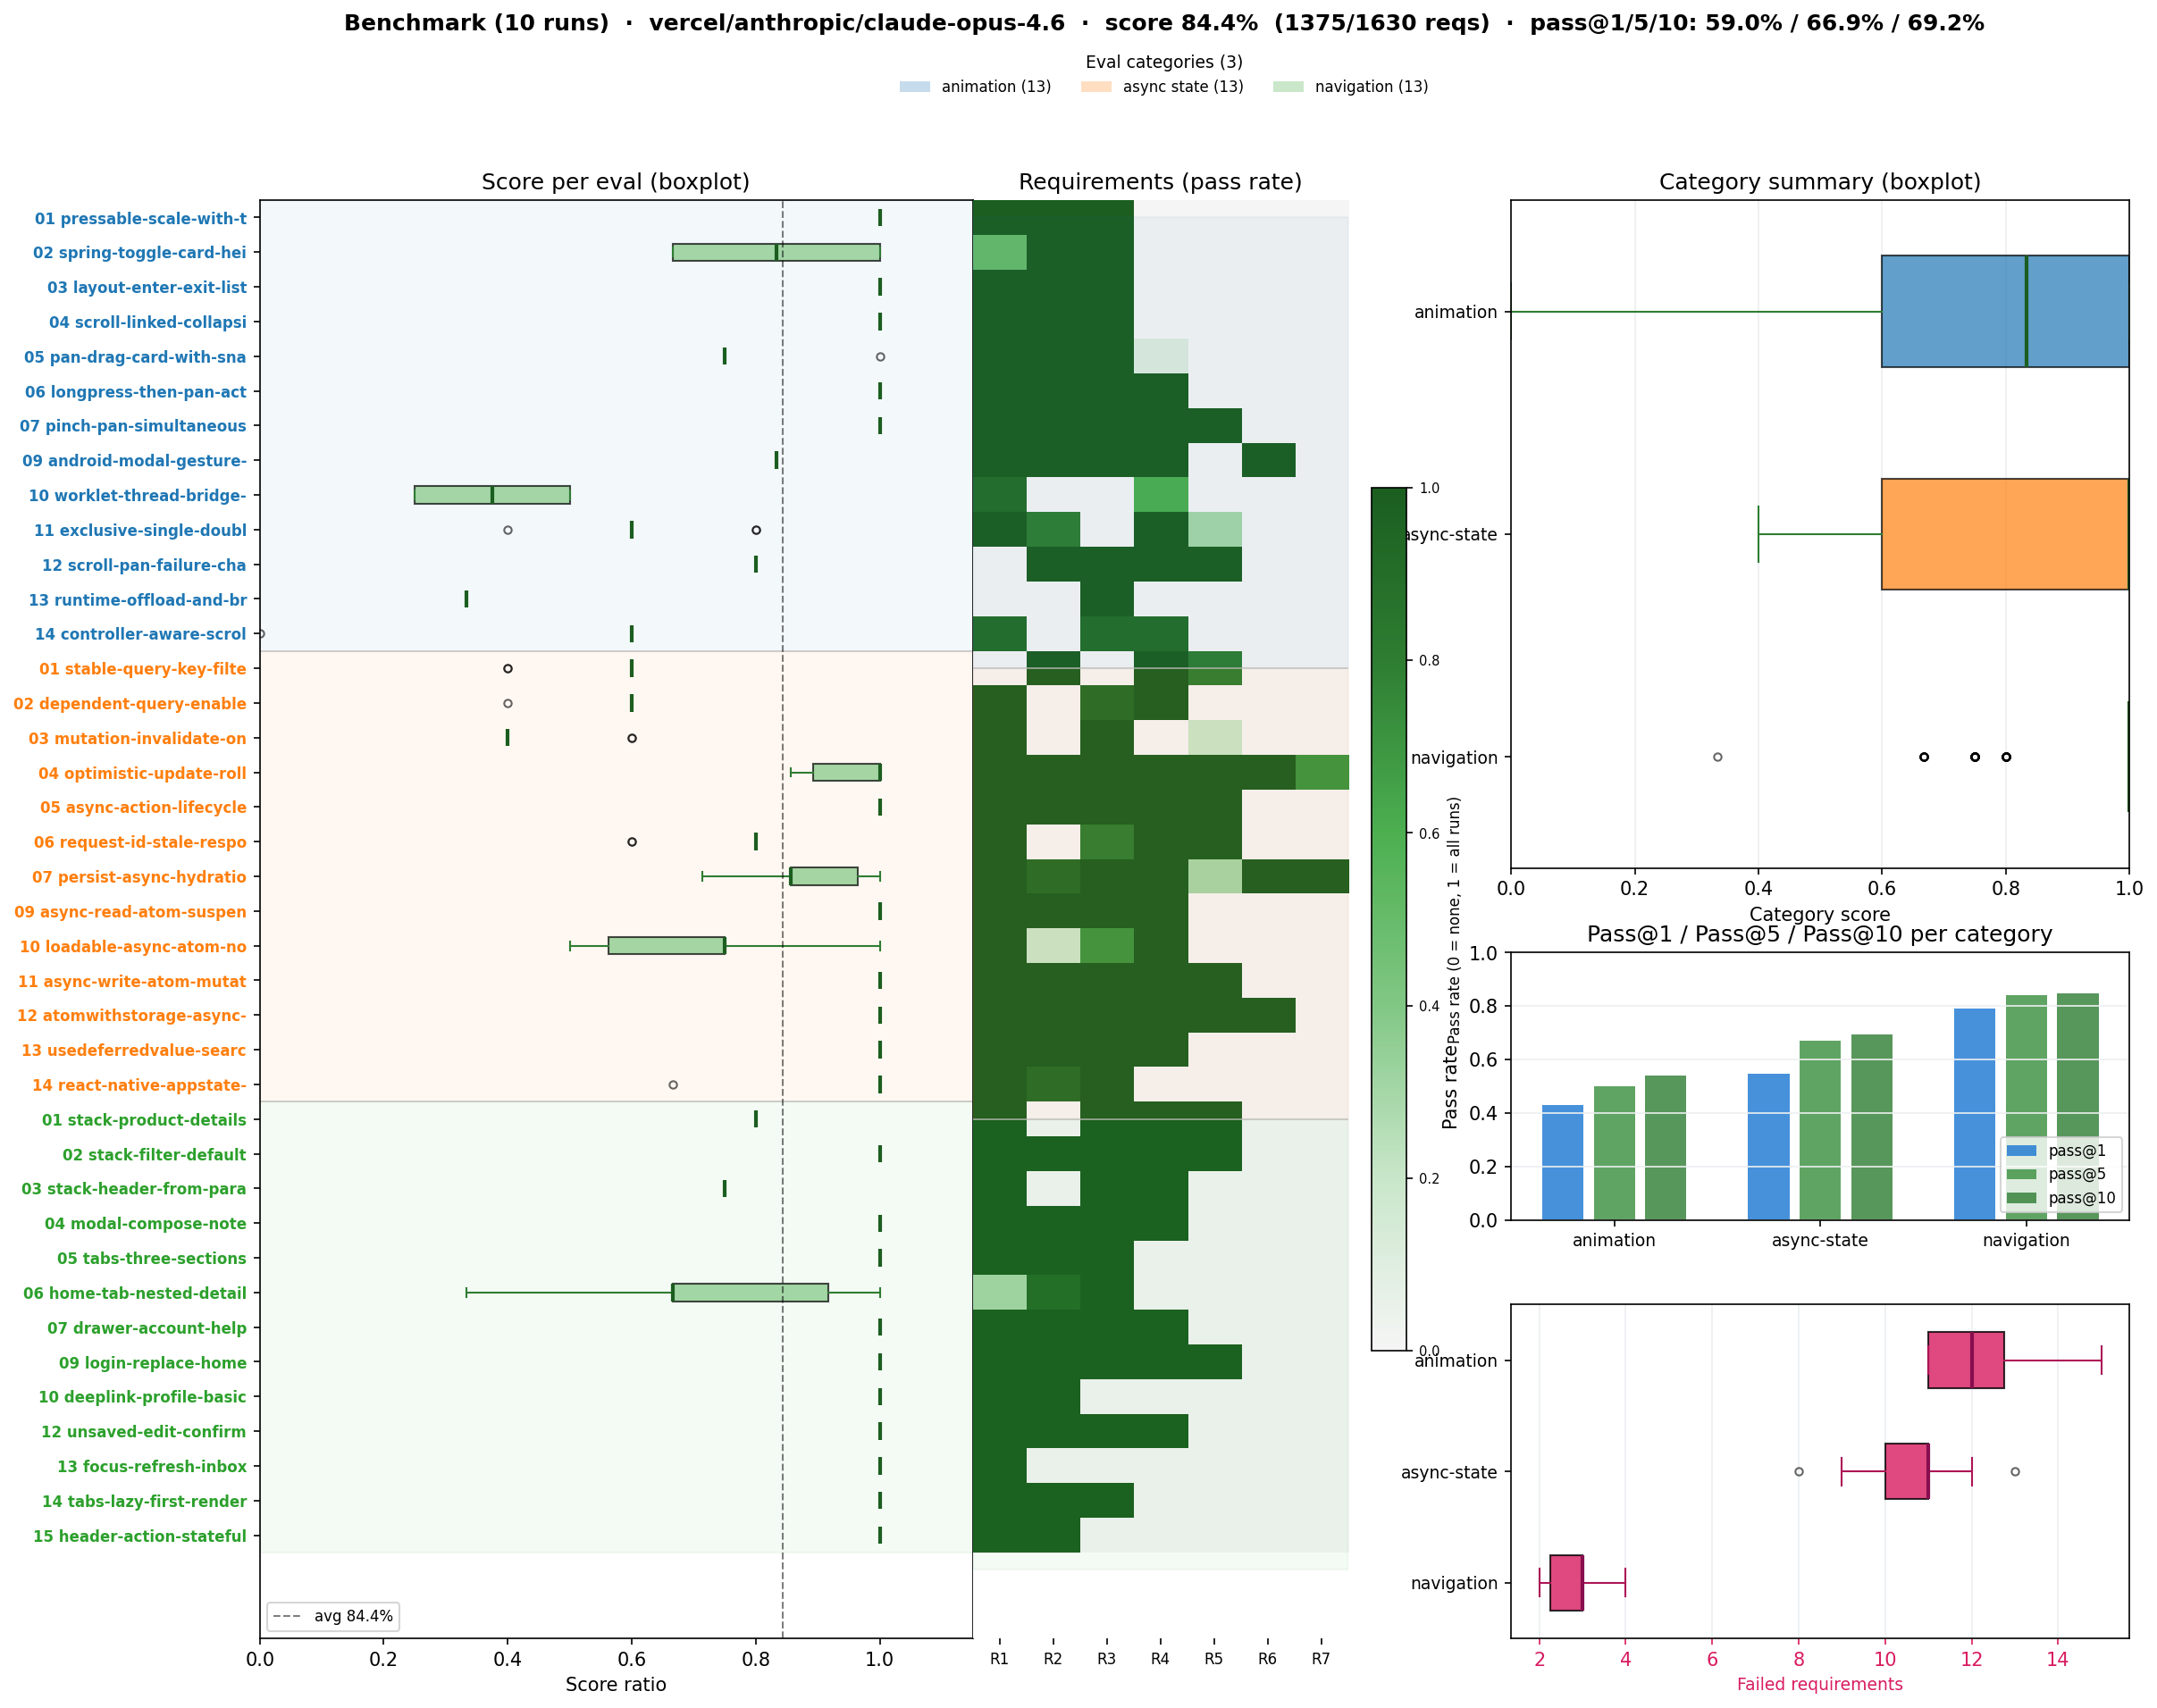
\includegraphics[width=\textwidth]{export/figures/claude-opus-4.6_benchmark_plot.png}
\caption{Benchmark Plot for claude-opus-4.6.}
\end{figure}

\begin{figure}[htbp]
\centering
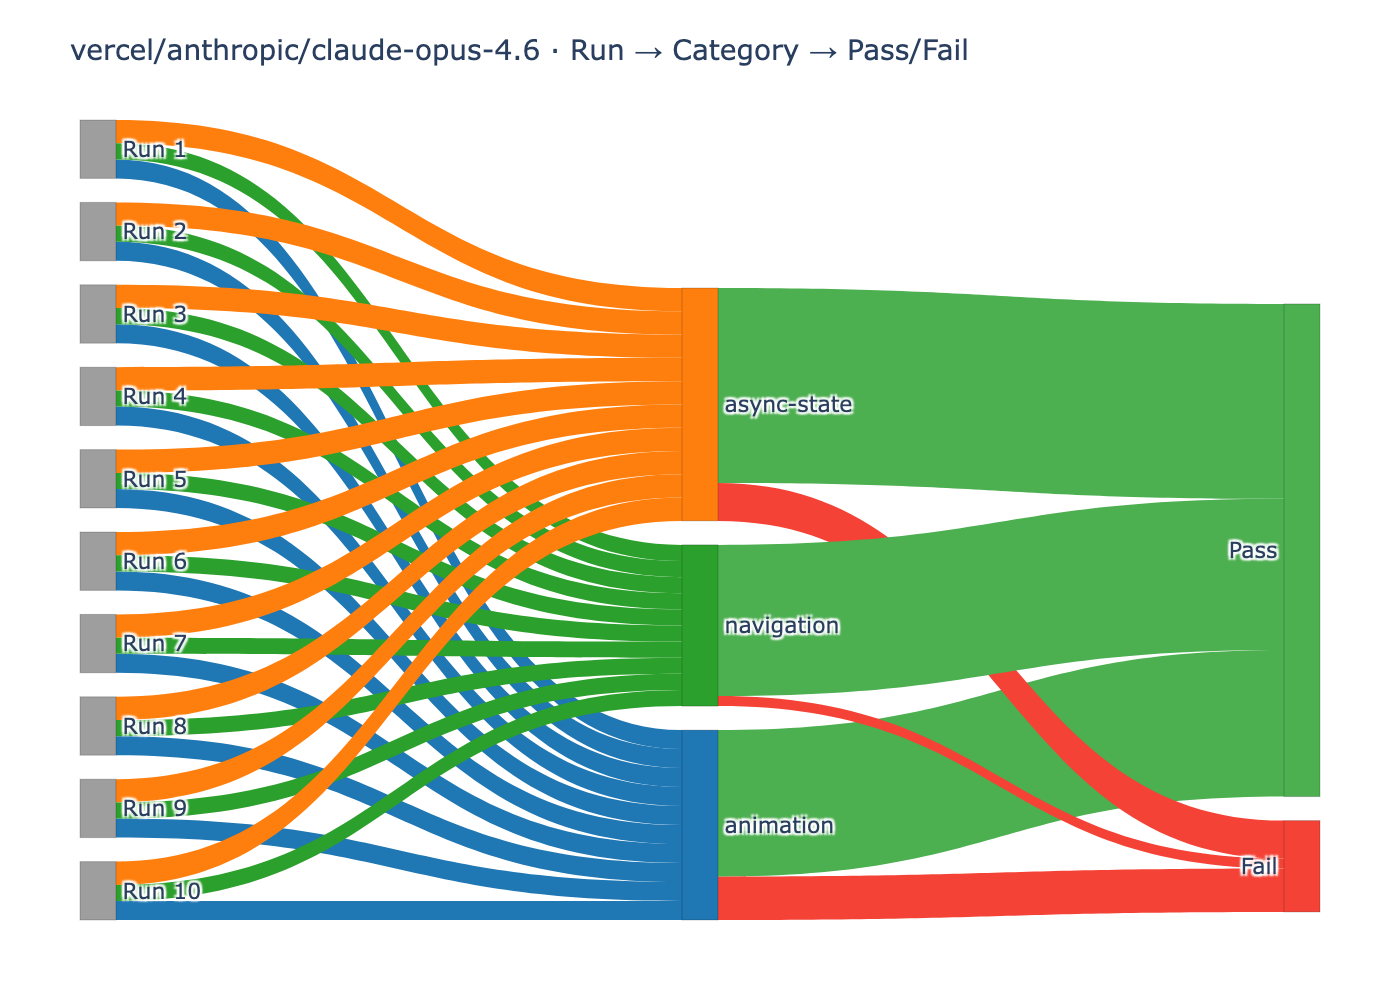
\includegraphics[width=\textwidth]{export/figures/claude-opus-4.6_sankey_per_run.png}
\caption{Sankey per run for claude-opus-4.6 showing the distribution of evals with respect to categories and results}
\end{figure}


\clearpage

\subsection{claude-sonnet-4.6}

% Table: summary
% Requires: \usepackage{booktabs}
\begin{table}[htbp]
\centering
\begin{tabular}{lrrrrrr}
\toprule
Model & Runs & Score & Reqs & P@1 & P@5 & P@10 \\
\midrule
vercel/anthropic/claude-sonnet-4.6 & 10 & 80.6\% & 2201/2730 & 55.0\% & 63.4\% & 66.7\% \\
\bottomrule
\end{tabular}
\caption{Model summary for claude-sonnet-4.6}
\end{table}


% Table: category_summary
% Requires: \usepackage{booktabs}
\begin{table}[htbp]
\centering
\begin{tabular}{lrrrr}
\toprule
Category & Score & Evals & Requirements & Failed requirements \\
\midrule
animation & 66.9\% & 130 & 53 & 191 \\
async state & 76.9\% & 130 & 65 & 139 \\
lists & 80.4\% & 180 & 79 & 151 \\
navigation & 93.8\% & 130 & 45 & 30 \\
react native apis & 93.3\% & 90 & 31 & 18 \\
\bottomrule
\end{tabular}
\caption{Results by category for claude-sonnet-4.6. Score: mean(per-eval passed/total weight) across evals and runs. Evals: count of evaluation tasks. Requirements: sum of requirement count per eval. Failed requirements: sum of failed requirement instances across runs.}
\end{table}


% Table: per_eval
% Requires: \usepackage{booktabs}
\begin{table}[htbp]
\centering
\begin{adjustbox}{width=0.8\textwidth}
\begin{tabular}{lrrrrr}
\toprule
Eval & Category & Score & P@1 & P@5 & P@10 \\
\midrule
01-rn-anim-pressable-scale-with-timing & animation & 100.0\% & 100.0\% & 100.0\% & 100.0\% \\
02-rn-anim-spring-toggle-card-height & animation & 80.0\% & 50.0\% & 99.6\% & 100.0\% \\
03-rn-anim-layout-enter-exit-list-items & animation & 100.0\% & 100.0\% & 100.0\% & 100.0\% \\
04-rn-anim-scroll-linked-collapsing-header & animation & 86.7\% & 60.0\% & 100.0\% & 100.0\% \\
05-rn-anim-pan-drag-card-with-snap-points & animation & 70.0\% & 0.0\% & 0.0\% & 0.0\% \\
06-rn-anim-longpress-then-pan-activation-gate & animation & 87.5\% & 50.0\% & 99.6\% & 100.0\% \\
07-rn-anim-pinch-pan-simultaneous-photo-canvas & animation & 100.0\% & 100.0\% & 100.0\% & 100.0\% \\
09-rn-anim-android-modal-gesture-root-safety & animation & 40.0\% & 0.0\% & 0.0\% & 0.0\% \\
10-rn-anim-worklet-thread-bridge-schedule-on-rn & animation & 40.0\% & 0.0\% & 0.0\% & 0.0\% \\
11-rn-rngh-exclusive-single-double-tap & animation & 54.0\% & 0.0\% & 0.0\% & 0.0\% \\
12-rn-rngh-scroll-pan-failure-chain & animation & 52.0\% & 0.0\% & 0.0\% & 0.0\% \\
13-rn-worklets-runtime-offload-and-bridge & animation & 33.3\% & 0.0\% & 0.0\% & 0.0\% \\
14-rn-keyboard-controller-aware-scroll-footer & animation & 26.0\% & 0.0\% & 0.0\% & 0.0\% \\
01-rn-rq-stable-query-key-filters & async state & 46.0\% & 0.0\% & 0.0\% & 0.0\% \\
02-rn-rq-dependent-query-enabled-gate & async state & 36.0\% & 0.0\% & 0.0\% & 0.0\% \\
03-rn-rq-mutation-invalidate-on-success & async state & 72.0\% & 0.0\% & 0.0\% & 0.0\% \\
04-rn-rq-optimistic-update-rollback & async state & 95.7\% & 90.0\% & 100.0\% & 100.0\% \\
05-rn-zustand-async-action-lifecycle & async state & 100.0\% & 100.0\% & 100.0\% & 100.0\% \\
06-rn-zustand-request-id-stale-response-guard & async state & 80.0\% & 0.0\% & 0.0\% & 0.0\% \\
07-rn-zustand-persist-async-hydration-gate & async state & 80.0\% & 10.0\% & 50.0\% & 100.0\% \\
09-rn-jotai-async-read-atom-suspense & async state & 90.0\% & 80.0\% & 100.0\% & 100.0\% \\
10-rn-jotai-loadable-async-atom-no-suspense & async state & 65.0\% & 0.0\% & 0.0\% & 0.0\% \\
11-rn-jotai-async-write-atom-mutation & async state & 100.0\% & 100.0\% & 100.0\% & 100.0\% \\
12-rn-jotai-atomwithstorage-async-rehydrate-guard & async state & 95.0\% & 70.0\% & 100.0\% & 100.0\% \\
13-rn-react-usedeferredvalue-search-stale-indicator & async state & 100.0\% & 100.0\% & 100.0\% & 100.0\% \\
14-rn-rq-react-native-appstate-focus-online-managers & async state & 40.0\% & 0.0\% & 0.0\% & 0.0\% \\
01-rn-flatlist-scroll-to-unread-fixed-rows & lists & 92.0\% & 80.0\% & 100.0\% & 100.0\% \\
02-rn-flatlist-basic-contact-list & lists & 100.0\% & 100.0\% & 100.0\% & 100.0\% \\
03-rn-flatlist-two-column-product-grid & lists & 100.0\% & 100.0\% & 100.0\% & 100.0\% \\
04-rn-flatlist-viewability-impression-tracking & lists & 80.0\% & 0.0\% & 0.0\% & 0.0\% \\
05-rn-flatlist-large-feed-window-tuning & lists & 100.0\% & 100.0\% & 100.0\% & 100.0\% \\
06-rn-flatlist-pull-to-refresh-feed & lists & 100.0\% & 100.0\% & 100.0\% & 100.0\% \\
07-rn-flatlist-to-sectionlist-conversion & lists & 100.0\% & 100.0\% & 100.0\% & 100.0\% \\
08-rn-flashlist-basic-list & lists & 100.0\% & 100.0\% & 100.0\% & 100.0\% \\
09-rn-flashlist-horizontal-rail-list-header & lists & 82.5\% & 30.0\% & 91.7\% & 100.0\% \\
10-rn-flashlist-horizontal-dynamic-height-header-first-item & lists & 88.3\% & 30.0\% & 91.7\% & 100.0\% \\
11-rn-flashlist-expandable-cards-layout-state & lists & 53.3\% & 0.0\% & 0.0\% & 0.0\% \\
12-rn-flashlist-chat-start-from-bottom & lists & 40.0\% & 0.0\% & 0.0\% & 0.0\% \\
13-rn-flashlist-masonry-photo-gallery & lists & 54.0\% & 0.0\% & 0.0\% & 0.0\% \\
14-rn-flatlist-to-legendlist-migration & lists & 46.7\% & 0.0\% & 0.0\% & 0.0\% \\
15-rn-legendlist-sticky-grouped-agenda & lists & 80.0\% & 0.0\% & 0.0\% & 0.0\% \\
16-rn-legendlist-section-scroll-to-location & lists & 100.0\% & 100.0\% & 100.0\% & 100.0\% \\
17-rn-legendlist-chat-start-from-bottom & lists & 80.0\% & 0.0\% & 0.0\% & 0.0\% \\
18-rn-legendlist-expandable-cards-recycling-state & lists & 50.0\% & 0.0\% & 0.0\% & 0.0\% \\
01-rn-nav-stack-product-details & navigation & 82.0\% & 10.0\% & 50.0\% & 100.0\% \\
02-rn-nav-stack-filter-default & navigation & 100.0\% & 100.0\% & 100.0\% & 100.0\% \\
03-rn-nav-stack-header-from-param & navigation & 77.5\% & 10.0\% & 50.0\% & 100.0\% \\
04-rn-nav-modal-compose-note & navigation & 100.0\% & 100.0\% & 100.0\% & 100.0\% \\
05-rn-nav-tabs-three-sections & navigation & 100.0\% & 100.0\% & 100.0\% & 100.0\% \\
06-rn-nav-home-tab-nested-details & navigation & 70.0\% & 10.0\% & 50.0\% & 100.0\% \\
07-rn-nav-drawer-account-help & navigation & 100.0\% & 100.0\% & 100.0\% & 100.0\% \\
09-rn-nav-login-replace-home & navigation & 100.0\% & 100.0\% & 100.0\% & 100.0\% \\
10-rn-nav-deeplink-profile-basic & navigation & 100.0\% & 100.0\% & 100.0\% & 100.0\% \\
12-rn-nav-unsaved-edit-confirm & navigation & 95.0\% & 80.0\% & 100.0\% & 100.0\% \\
13-rn-nav-focus-refresh-inbox & navigation & 100.0\% & 100.0\% & 100.0\% & 100.0\% \\
14-rn-nav-tabs-lazy-first-render & navigation & 100.0\% & 100.0\% & 100.0\% & 100.0\% \\
15-rn-nav-header-action-stateful & navigation & 95.0\% & 90.0\% & 100.0\% & 100.0\% \\
01-rn-stylesheet-card-variants & react native apis & 100.0\% & 100.0\% & 100.0\% & 100.0\% \\
02-rn-stylesheet-absolute-fill-overlay-badge & react native apis & 50.0\% & 0.0\% & 0.0\% & 0.0\% \\
03-rn-stylesheet-divider-hairline & react native apis & 90.0\% & 80.0\% & 100.0\% & 100.0\% \\
04-rn-image-network-dimensions & react native apis & 100.0\% & 100.0\% & 100.0\% & 100.0\% \\
05-rn-imagebackground-resize-mode & react native apis & 100.0\% & 100.0\% & 100.0\% & 100.0\% \\
06-rn-platform-select-small-style-delta & react native apis & 100.0\% & 100.0\% & 100.0\% & 100.0\% \\
07-rn-platform-os-conditional-cta & react native apis & 100.0\% & 100.0\% & 100.0\% & 100.0\% \\
08-rn-platform-file-extension-component-split & react native apis & 100.0\% & 100.0\% & 100.0\% & 100.0\% \\
09-rn-keyboardavoidingview-login-form & react native apis & 100.0\% & 100.0\% & 100.0\% & 100.0\% \\
\bottomrule
\end{tabular}
\end{adjustbox}
\caption{Per-eval results (score and pass@k) for claude-sonnet-4.6}
\end{table}


\begin{figure}[htbp]
\centering
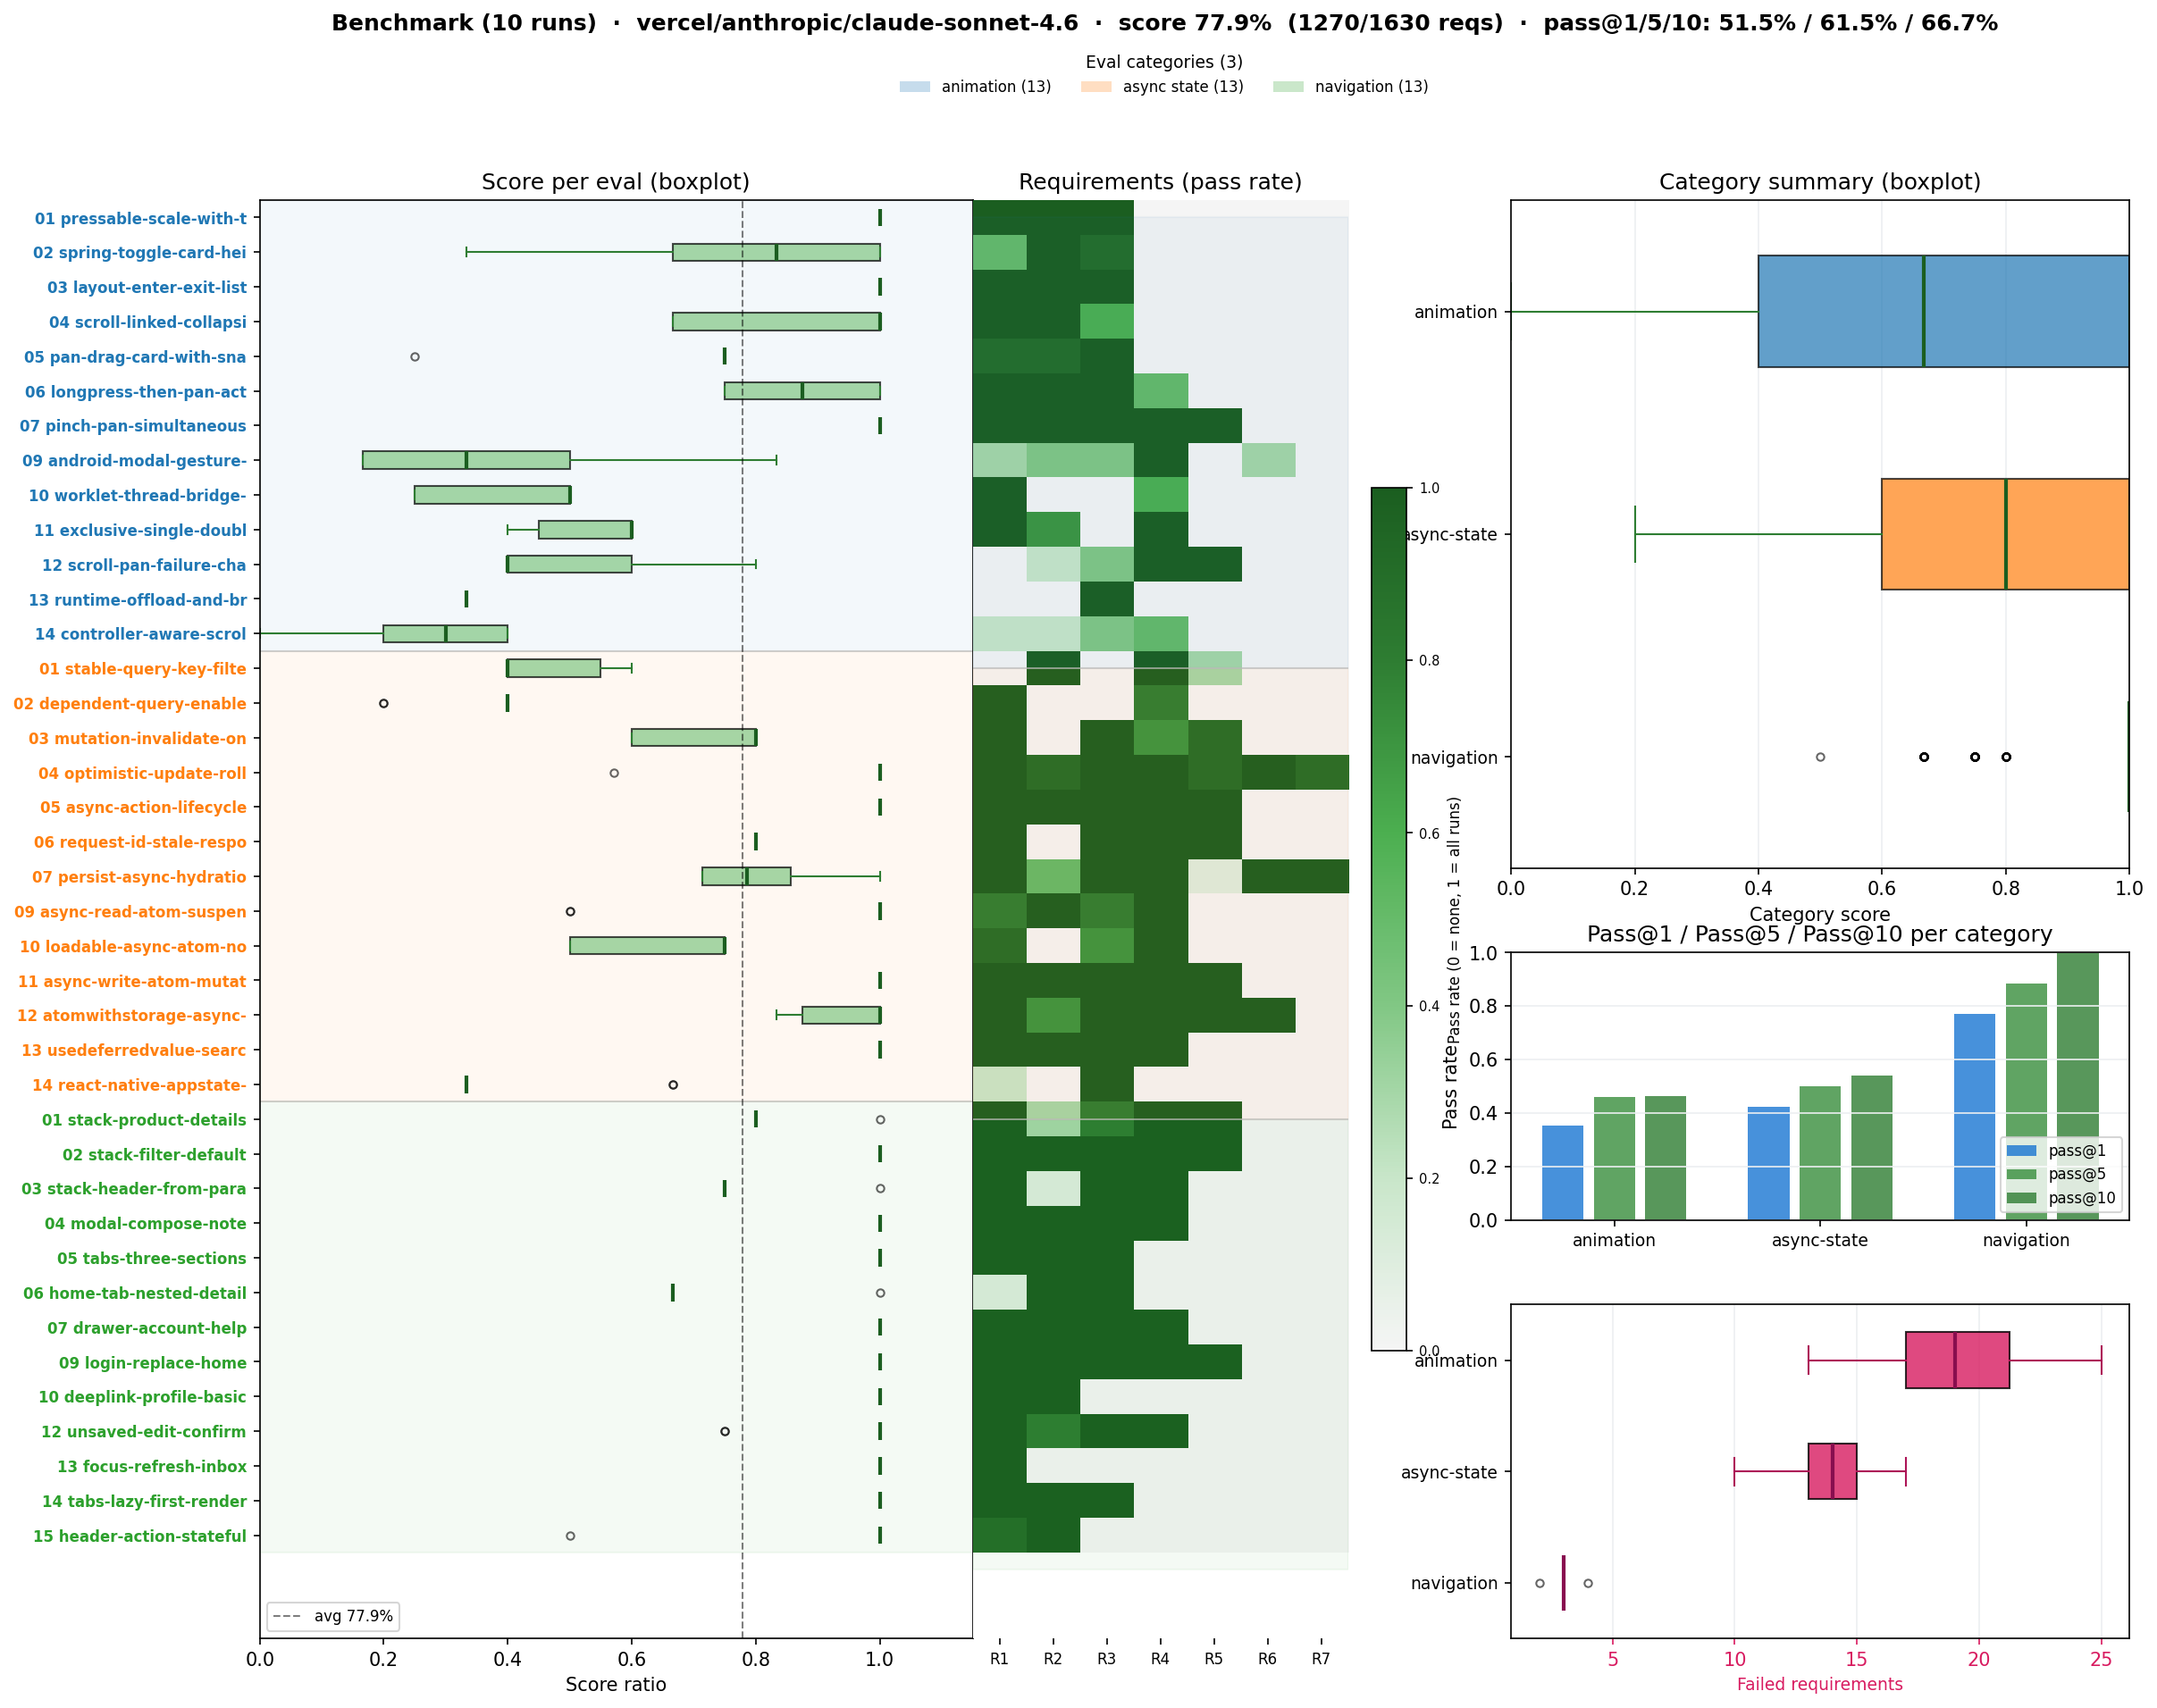
\includegraphics[width=\textwidth]{export/figures/claude-sonnet-4.6_benchmark_plot.png}
\caption{Benchmark Plot for claude-sonnet-4.6.}
\end{figure}

\begin{figure}[htbp]
\centering
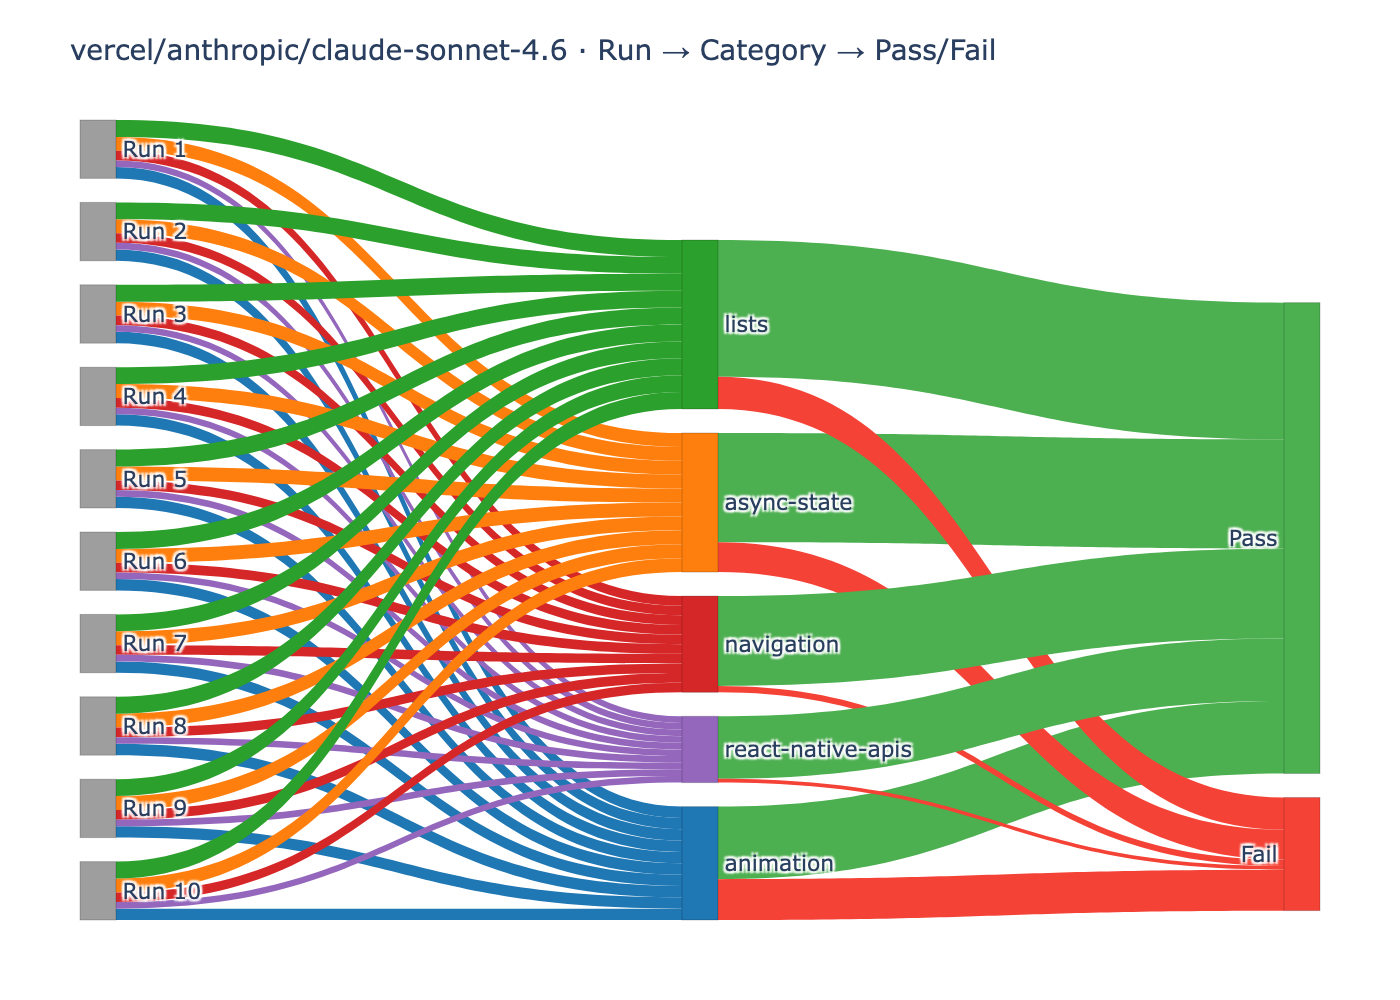
\includegraphics[width=\textwidth]{export/figures/claude-sonnet-4.6_sankey_per_run.png}
\caption{Sankey per run for claude-sonnet-4.6 showing the distribution of evals with respect to categories and results}
\end{figure}


\clearpage

\subsection{deepseek-r1-distill-qwen-32b}

% Table: summary
% Requires: \usepackage{booktabs}
\begin{table}[htbp]
\centering
\begin{tabular}{lrrrrrr}
\toprule
Model & Runs & Score & Reqs & P@1 & P@5 & P@10 \\
\midrule
cloudflare-ai-gateway/workers-ai/@cf/deepseek-ai/d & 10 & 44.4\% & 1211/2730 & 19.2\% & 31.1\% & 36.4\% \\
\bottomrule
\end{tabular}
\caption{Model summary for deepseek-r1-distill-qwen-32b}
\end{table}


% Table: category_summary
% Requires: \usepackage{booktabs}
\begin{table}[htbp]
\centering
\begin{tabular}{lrrrr}
\toprule
Category & Score & Evals & Requirements & Failed requirements \\
\midrule
animation & 11.1\% & 130 & 53 & 483 \\
async state & 32.7\% & 130 & 65 & 438 \\
lists & 55.7\% & 180 & 79 & 356 \\
navigation & 57.3\% & 130 & 45 & 190 \\
react native apis & 82.1\% & 90 & 31 & 52 \\
\bottomrule
\end{tabular}
\caption{Results by category for deepseek-r1-distill-qwen-32b. Score: mean(per-eval passed/total weight) across evals and runs. Evals: count of evaluation tasks. Requirements: sum of requirement count per eval. Failed requirements: sum of failed requirement instances across runs.}
\end{table}


% Table: per_eval
% Requires: \usepackage{booktabs}
\begin{table}[htbp]
\centering
\begin{adjustbox}{width=0.8\textwidth}
\begin{tabular}{lrrrrr}
\toprule
Eval & Category & Score & P@1 & P@5 & P@10 \\
\midrule
01-rn-anim-pressable-scale-with-timing & animation & 53.3\% & 10.0\% & 50.0\% & 100.0\% \\
02-rn-anim-spring-toggle-card-height & animation & 6.7\% & 0.0\% & 0.0\% & 0.0\% \\
03-rn-anim-layout-enter-exit-list-items & animation & 40.0\% & 10.0\% & 50.0\% & 100.0\% \\
04-rn-anim-scroll-linked-collapsing-header & animation & 6.7\% & 0.0\% & 0.0\% & 0.0\% \\
05-rn-anim-pan-drag-card-with-snap-points & animation & 2.5\% & 0.0\% & 0.0\% & 0.0\% \\
06-rn-anim-longpress-then-pan-activation-gate & animation & 7.5\% & 0.0\% & 0.0\% & 0.0\% \\
07-rn-anim-pinch-pan-simultaneous-photo-canvas & animation & 4.0\% & 0.0\% & 0.0\% & 0.0\% \\
09-rn-anim-android-modal-gesture-root-safety & animation & 5.0\% & 0.0\% & 0.0\% & 0.0\% \\
10-rn-anim-worklet-thread-bridge-schedule-on-rn & animation & 0.0\% & 0.0\% & 0.0\% & 0.0\% \\
11-rn-rngh-exclusive-single-double-tap & animation & 0.0\% & 0.0\% & 0.0\% & 0.0\% \\
12-rn-rngh-scroll-pan-failure-chain & animation & 0.0\% & 0.0\% & 0.0\% & 0.0\% \\
13-rn-worklets-runtime-offload-and-bridge & animation & 16.7\% & 0.0\% & 0.0\% & 0.0\% \\
14-rn-keyboard-controller-aware-scroll-footer & animation & 2.0\% & 0.0\% & 0.0\% & 0.0\% \\
01-rn-rq-stable-query-key-filters & async state & 6.0\% & 0.0\% & 0.0\% & 0.0\% \\
02-rn-rq-dependent-query-enabled-gate & async state & 18.0\% & 0.0\% & 0.0\% & 0.0\% \\
03-rn-rq-mutation-invalidate-on-success & async state & 2.0\% & 0.0\% & 0.0\% & 0.0\% \\
04-rn-rq-optimistic-update-rollback & async state & 11.4\% & 0.0\% & 0.0\% & 0.0\% \\
05-rn-zustand-async-action-lifecycle & async state & 86.0\% & 50.0\% & 99.6\% & 100.0\% \\
06-rn-zustand-request-id-stale-response-guard & async state & 40.0\% & 0.0\% & 0.0\% & 0.0\% \\
07-rn-zustand-persist-async-hydration-gate & async state & 28.6\% & 0.0\% & 0.0\% & 0.0\% \\
09-rn-jotai-async-read-atom-suspense & async state & 57.5\% & 20.0\% & 77.8\% & 100.0\% \\
10-rn-jotai-loadable-async-atom-no-suspense & async state & 0.0\% & 0.0\% & 0.0\% & 0.0\% \\
11-rn-jotai-async-write-atom-mutation & async state & 38.0\% & 0.0\% & 0.0\% & 0.0\% \\
12-rn-jotai-atomwithstorage-async-rehydrate-guard & async state & 68.3\% & 0.0\% & 0.0\% & 0.0\% \\
13-rn-react-usedeferredvalue-search-stale-indicator & async state & 42.5\% & 10.0\% & 50.0\% & 100.0\% \\
14-rn-rq-react-native-appstate-focus-online-managers & async state & 26.7\% & 0.0\% & 0.0\% & 0.0\% \\
01-rn-flatlist-scroll-to-unread-fixed-rows & lists & 44.0\% & 0.0\% & 0.0\% & 0.0\% \\
02-rn-flatlist-basic-contact-list & lists & 100.0\% & 100.0\% & 100.0\% & 100.0\% \\
03-rn-flatlist-two-column-product-grid & lists & 93.3\% & 80.0\% & 100.0\% & 100.0\% \\
04-rn-flatlist-viewability-impression-tracking & lists & 66.0\% & 0.0\% & 0.0\% & 0.0\% \\
05-rn-flatlist-large-feed-window-tuning & lists & 60.0\% & 0.0\% & 0.0\% & 0.0\% \\
06-rn-flatlist-pull-to-refresh-feed & lists & 80.0\% & 0.0\% & 0.0\% & 0.0\% \\
07-rn-flatlist-to-sectionlist-conversion & lists & 88.0\% & 40.0\% & 97.6\% & 100.0\% \\
08-rn-flashlist-basic-list & lists & 76.7\% & 50.0\% & 99.6\% & 100.0\% \\
09-rn-flashlist-horizontal-rail-list-header & lists & 42.5\% & 0.0\% & 0.0\% & 0.0\% \\
10-rn-flashlist-horizontal-dynamic-height-header-first-item & lists & 53.3\% & 0.0\% & 0.0\% & 0.0\% \\
11-rn-flashlist-expandable-cards-layout-state & lists & 36.7\% & 0.0\% & 0.0\% & 0.0\% \\
12-rn-flashlist-chat-start-from-bottom & lists & 34.0\% & 0.0\% & 0.0\% & 0.0\% \\
13-rn-flashlist-masonry-photo-gallery & lists & 52.0\% & 0.0\% & 0.0\% & 0.0\% \\
14-rn-flatlist-to-legendlist-migration & lists & 20.0\% & 0.0\% & 0.0\% & 0.0\% \\
15-rn-legendlist-sticky-grouped-agenda & lists & 48.0\% & 0.0\% & 0.0\% & 0.0\% \\
16-rn-legendlist-section-scroll-to-location & lists & 52.0\% & 10.0\% & 50.0\% & 100.0\% \\
17-rn-legendlist-chat-start-from-bottom & lists & 28.0\% & 0.0\% & 0.0\% & 0.0\% \\
18-rn-legendlist-expandable-cards-recycling-state & lists & 27.5\% & 0.0\% & 0.0\% & 0.0\% \\
01-rn-nav-stack-product-details & navigation & 60.0\% & 0.0\% & 0.0\% & 0.0\% \\
02-rn-nav-stack-filter-default & navigation & 98.0\% & 90.0\% & 100.0\% & 100.0\% \\
03-rn-nav-stack-header-from-param & navigation & 50.0\% & 0.0\% & 0.0\% & 0.0\% \\
04-rn-nav-modal-compose-note & navigation & 82.5\% & 40.0\% & 97.6\% & 100.0\% \\
05-rn-nav-tabs-three-sections & navigation & 60.0\% & 30.0\% & 91.7\% & 100.0\% \\
06-rn-nav-home-tab-nested-details & navigation & 70.0\% & 30.0\% & 91.7\% & 100.0\% \\
07-rn-nav-drawer-account-help & navigation & 45.0\% & 10.0\% & 50.0\% & 100.0\% \\
09-rn-nav-login-replace-home & navigation & 22.0\% & 0.0\% & 0.0\% & 0.0\% \\
10-rn-nav-deeplink-profile-basic & navigation & 25.0\% & 10.0\% & 50.0\% & 100.0\% \\
12-rn-nav-unsaved-edit-confirm & navigation & 52.5\% & 0.0\% & 0.0\% & 0.0\% \\
13-rn-nav-focus-refresh-inbox & navigation & 100.0\% & 100.0\% & 100.0\% & 100.0\% \\
14-rn-nav-tabs-lazy-first-render & navigation & 80.0\% & 40.0\% & 97.6\% & 100.0\% \\
15-rn-nav-header-action-stateful & navigation & 0.0\% & 0.0\% & 0.0\% & 0.0\% \\
01-rn-stylesheet-card-variants & react native apis & 76.7\% & 50.0\% & 99.6\% & 100.0\% \\
02-rn-stylesheet-absolute-fill-overlay-badge & react native apis & 66.7\% & 0.0\% & 0.0\% & 0.0\% \\
03-rn-stylesheet-divider-hairline & react native apis & 43.3\% & 0.0\% & 0.0\% & 0.0\% \\
04-rn-image-network-dimensions & react native apis & 100.0\% & 100.0\% & 100.0\% & 100.0\% \\
05-rn-imagebackground-resize-mode & react native apis & 62.5\% & 0.0\% & 0.0\% & 0.0\% \\
06-rn-platform-select-small-style-delta & react native apis & 100.0\% & 100.0\% & 100.0\% & 100.0\% \\
07-rn-platform-os-conditional-cta & react native apis & 100.0\% & 100.0\% & 100.0\% & 100.0\% \\
08-rn-platform-file-extension-component-split & react native apis & 100.0\% & 100.0\% & 100.0\% & 100.0\% \\
09-rn-keyboardavoidingview-login-form & react native apis & 90.0\% & 90.0\% & 100.0\% & 100.0\% \\
\bottomrule
\end{tabular}
\end{adjustbox}
\caption{Per-eval results (score and pass@k) for deepseek-r1-distill-qwen-32b}
\end{table}


\begin{figure}[htbp]
\centering
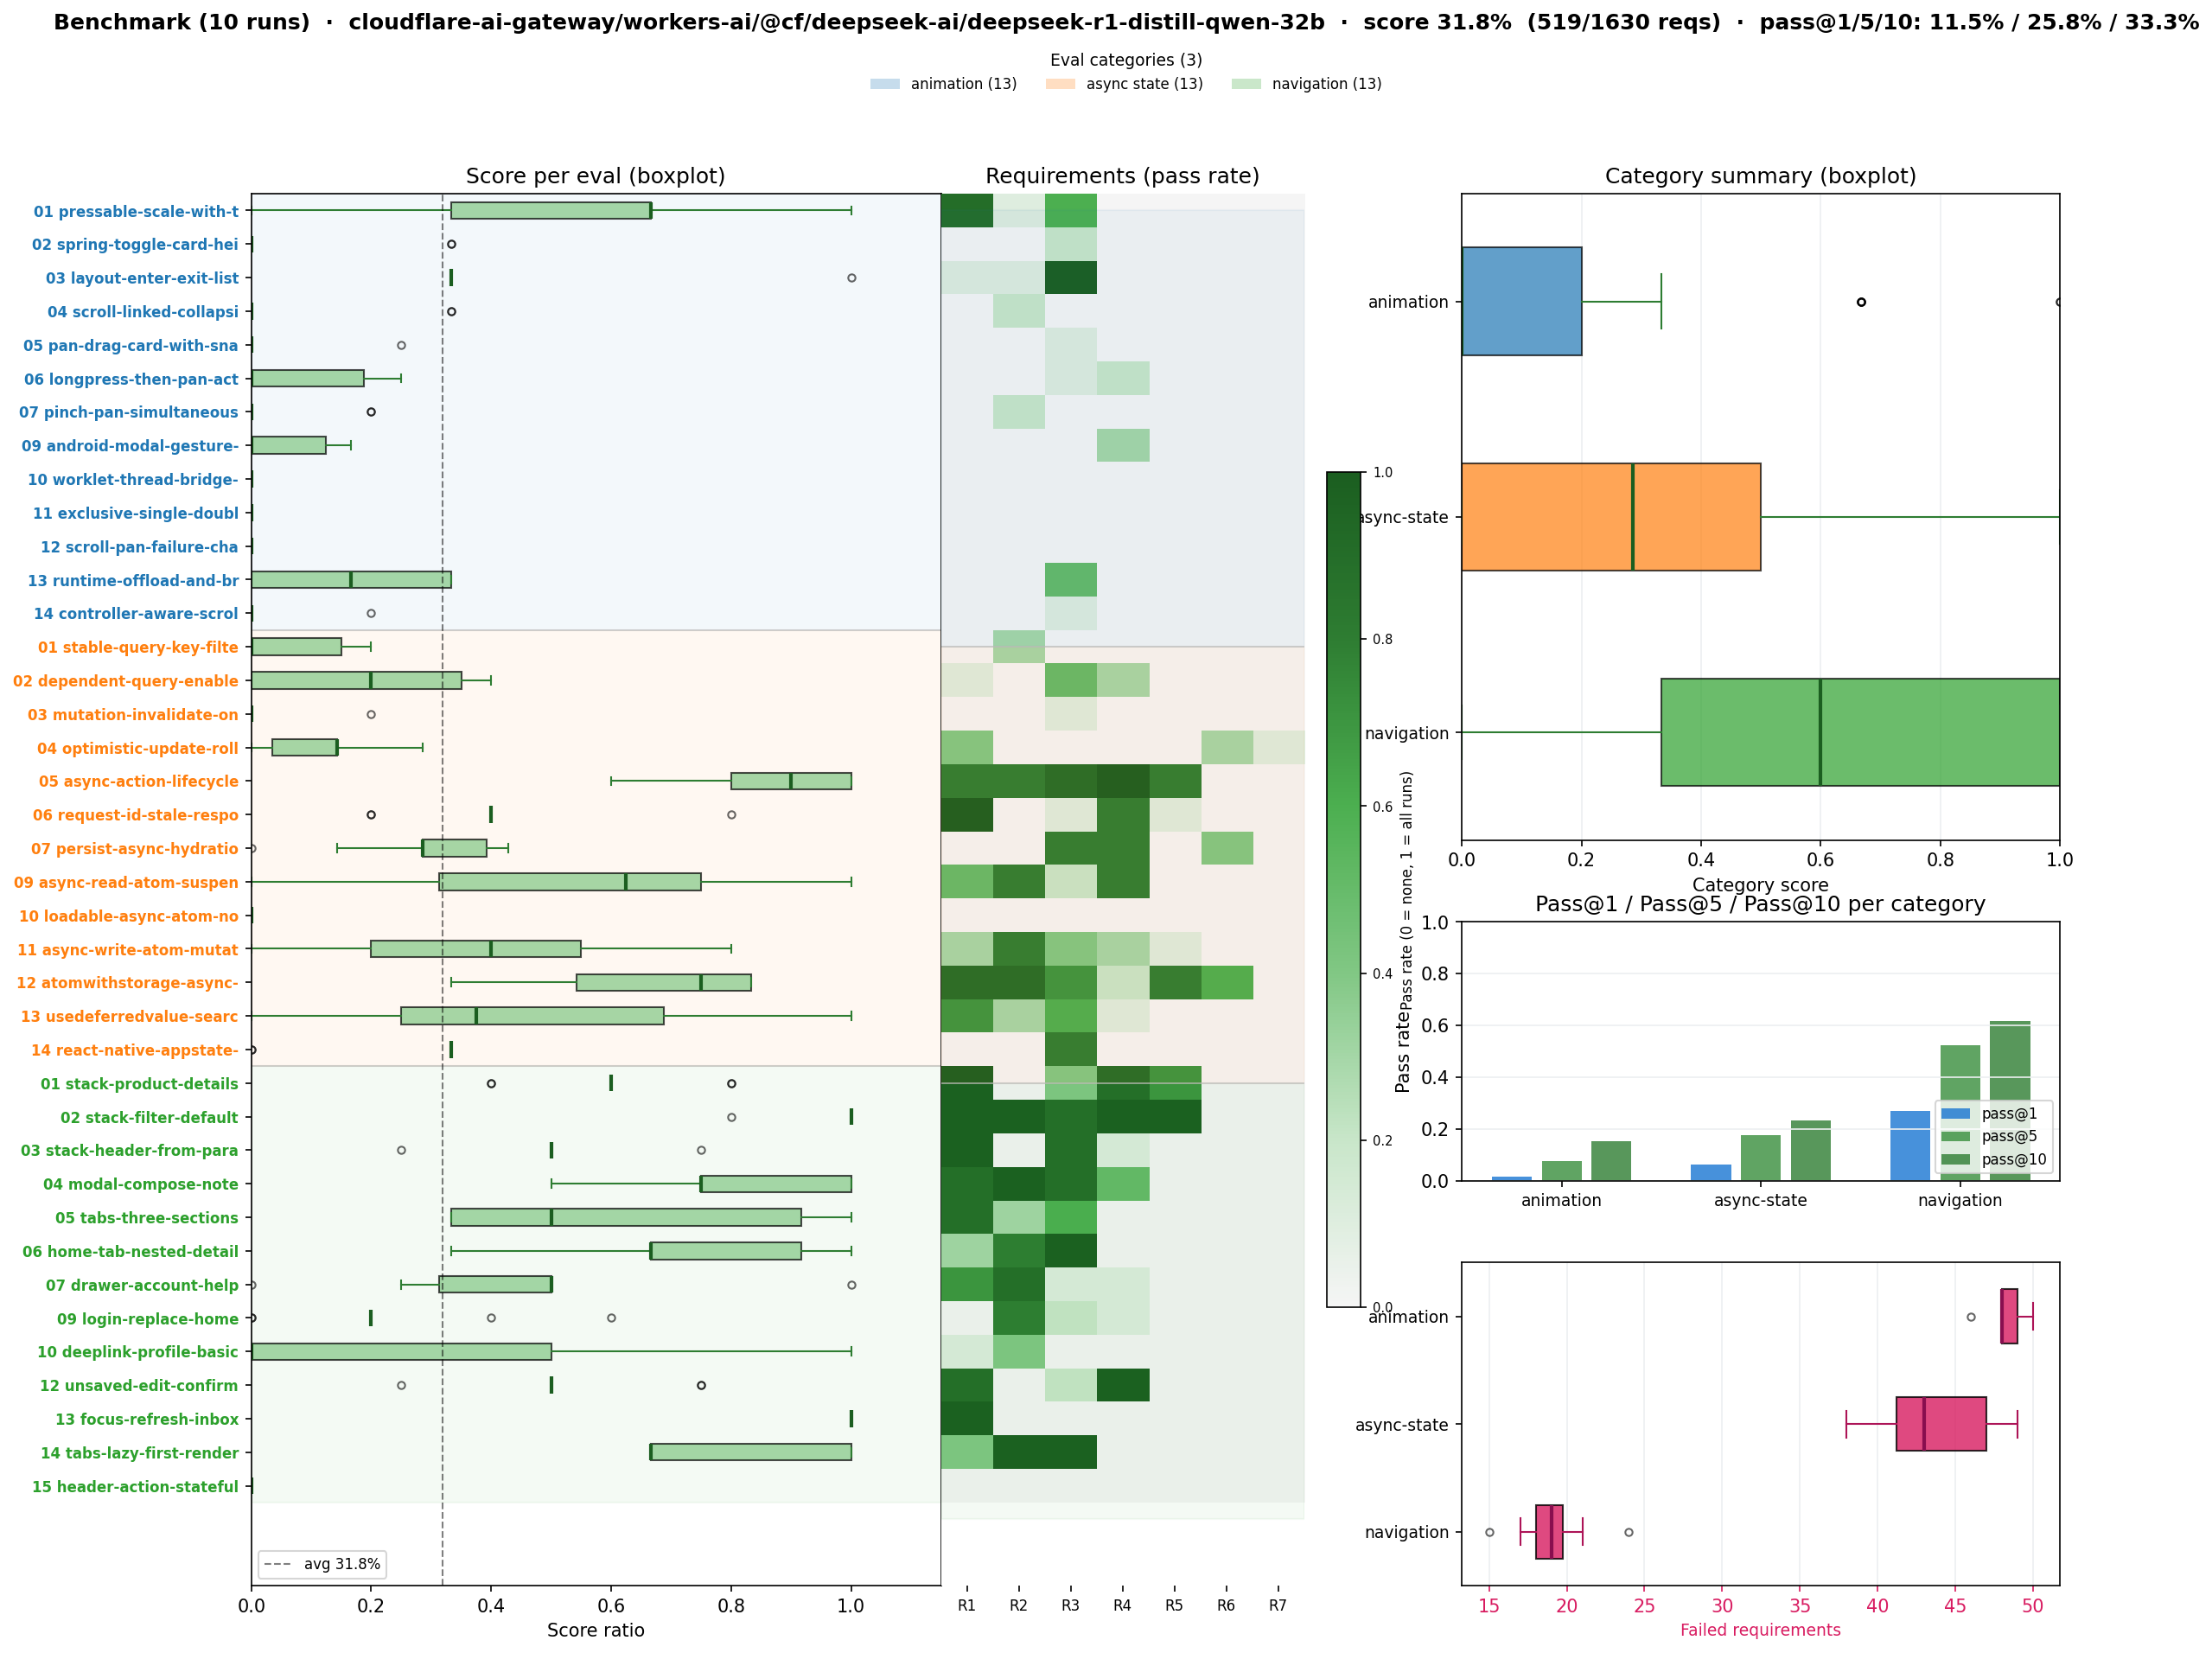
\includegraphics[width=\textwidth]{export/figures/deepseek-r1-distill-qwen-32b_benchmark_plot.png}
\caption{Benchmark Plot for deepseek-r1-distill-qwen-32b.}
\end{figure}

\begin{figure}[htbp]
\centering
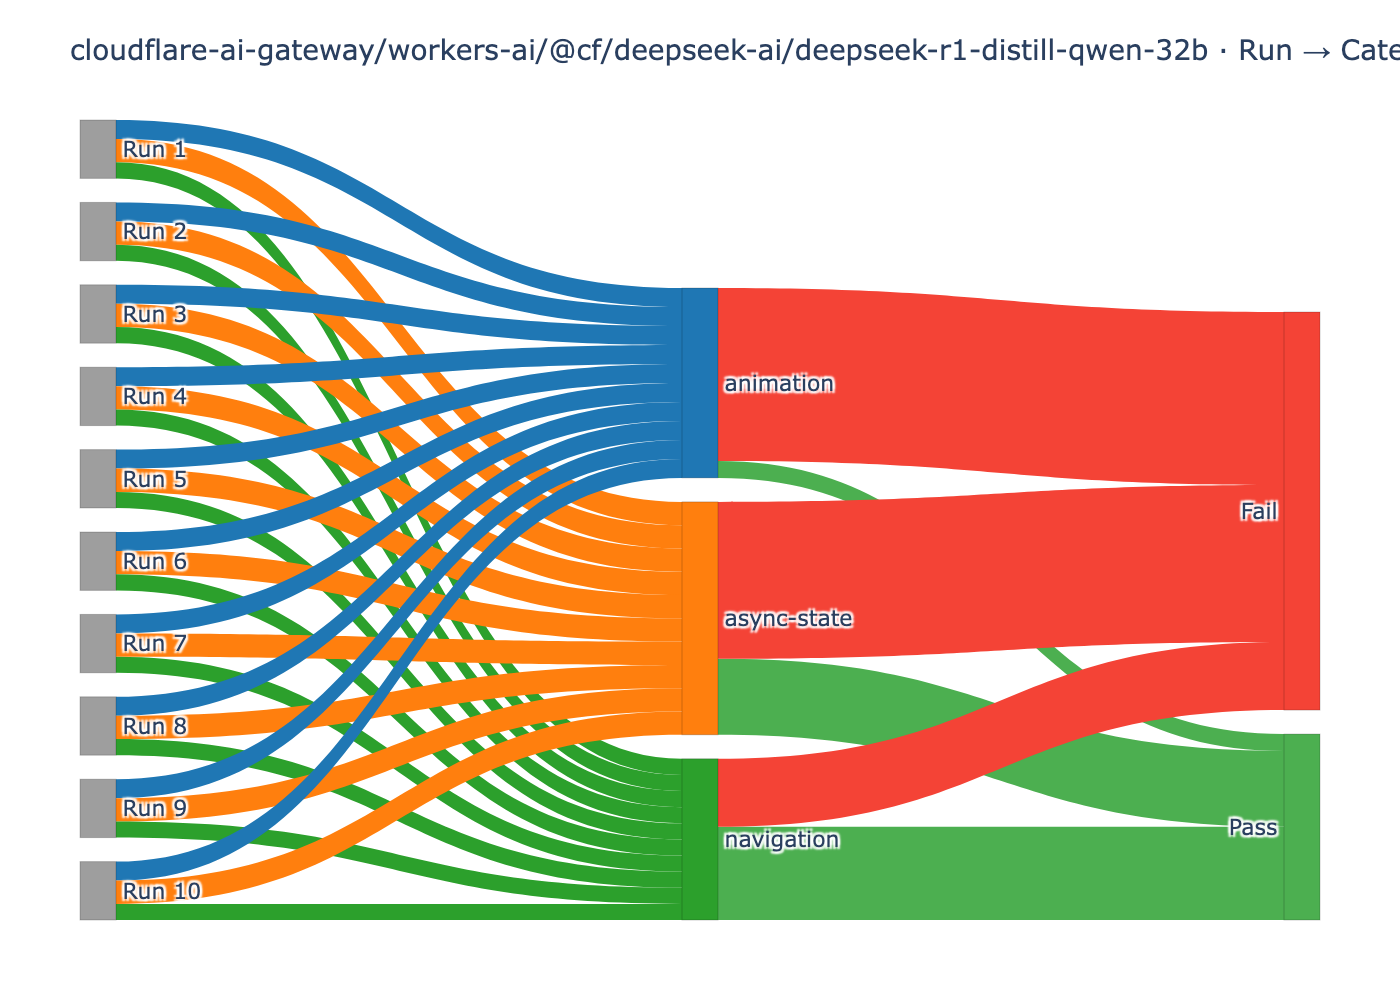
\includegraphics[width=\textwidth]{export/figures/deepseek-r1-distill-qwen-32b_sankey_per_run.png}
\caption{Sankey per run for deepseek-r1-distill-qwen-32b showing the distribution of evals with respect to categories and results}
\end{figure}


\clearpage

\subsection{deepseek-v3.2}

% Table: summary
% Requires: \usepackage{booktabs}
\begin{table}[htbp]
\centering
\begin{tabular}{lrrrrrr}
\toprule
Model & Runs & Score & Reqs & P@1 & P@5 & P@10 \\
\midrule
vercel/deepseek/deepseek-v3.2 & 10 & 69.0\% & 1118/1621 & 41.0\% & 56.8\% & 59.0\% \\
\bottomrule
\end{tabular}
\caption{Model summary for deepseek-v3.2}
\end{table}


% Table: category_summary
% Requires: \usepackage{booktabs}
\begin{table}[htbp]
\centering
\begin{tabular}{lrrrr}
\toprule
Category & Score & Evals & Requirements & Failed requirements \\
\midrule
animation & 57.5\% & 129 & 53 & 233 \\
async state & 71.0\% & 130 & 65 & 182 \\
lists & 68.5\% & 180 & 79 & 245 \\
navigation & 80.4\% & 129 & 45 & 88 \\
react native apis & 89.9\% & 90 & 31 & 28 \\
\bottomrule
\end{tabular}
\caption{Results by category for deepseek-v3.2. Score: mean(per-eval passed/total weight) across evals and runs. Evals: count of evaluation tasks. Requirements: sum of requirement count per eval. Failed requirements: sum of failed requirement instances across runs.}
\end{table}


% Table: per_eval
% Requires: \usepackage{booktabs}
\begin{table}[htbp]
\centering
\begin{tabular}{lrrrrr}
\toprule
Eval & Category & Score & P@1 & P@5 & P@10 \\
\midrule
01-rn-anim-pressable-scale-with-timing & animation & 70.0\% & 30.0\% & 91.7\% & 100.0\% \\
02-rn-anim-spring-toggle-card-height & animation & 66.7\% & 30.0\% & 91.7\% & 100.0\% \\
03-rn-anim-layout-enter-exit-list-items & animation & 86.7\% & 80.0\% & 100.0\% & 100.0\% \\
04-rn-anim-scroll-linked-collapsing-header & animation & 93.3\% & 90.0\% & 100.0\% & 100.0\% \\
05-rn-anim-pan-drag-card-with-snap-points & animation & 52.5\% & 0.0\% & 0.0\% & 0.0\% \\
06-rn-anim-longpress-then-pan-activation-gate & animation & 82.5\% & 50.0\% & 99.6\% & 100.0\% \\
07-rn-anim-pinch-pan-simultaneous-photo-canvas & animation & 98.0\% & 90.0\% & 100.0\% & 100.0\% \\
09-rn-anim-android-modal-gesture-root-safety & animation & 48.3\% & 0.0\% & 0.0\% & 0.0\% \\
10-rn-anim-worklet-thread-bridge-schedule-on-rn & animation & 22.2\% & 0.0\% & 0.0\% & 0.0\% \\
11-rn-rngh-exclusive-single-double-tap & animation & 30.0\% & 0.0\% & 0.0\% & 0.0\% \\
12-rn-rngh-scroll-pan-failure-chain & animation & 60.0\% & 0.0\% & 0.0\% & 0.0\% \\
13-rn-worklets-runtime-offload-and-bridge & animation & 20.0\% & 0.0\% & 0.0\% & 0.0\% \\
14-rn-keyboard-controller-aware-scroll-footer & animation & 14.0\% & 0.0\% & 0.0\% & 0.0\% \\
01-rn-rq-stable-query-key-filters & async state & 34.0\% & 0.0\% & 0.0\% & 0.0\% \\
02-rn-rq-dependent-query-enabled-gate & async state & 34.0\% & 0.0\% & 0.0\% & 0.0\% \\
03-rn-rq-mutation-invalidate-on-success & async state & 72.0\% & 0.0\% & 0.0\% & 0.0\% \\
04-rn-rq-optimistic-update-rollback & async state & 91.4\% & 60.0\% & 100.0\% & 100.0\% \\
05-rn-zustand-async-action-lifecycle & async state & 100.0\% & 100.0\% & 100.0\% & 100.0\% \\
06-rn-zustand-request-id-stale-response-guard & async state & 78.0\% & 30.0\% & 91.7\% & 100.0\% \\
07-rn-zustand-persist-async-hydration-gate & async state & 60.0\% & 0.0\% & 0.0\% & 0.0\% \\
09-rn-jotai-async-read-atom-suspense & async state & 92.5\% & 70.0\% & 100.0\% & 100.0\% \\
10-rn-jotai-loadable-async-atom-no-suspense & async state & 22.5\% & 0.0\% & 0.0\% & 0.0\% \\
11-rn-jotai-async-write-atom-mutation & async state & 94.0\% & 80.0\% & 100.0\% & 100.0\% \\
12-rn-jotai-atomwithstorage-async-rehydrate-guard & async state & 91.7\% & 50.0\% & 99.6\% & 100.0\% \\
13-rn-react-usedeferredvalue-search-stale-indicator & async state & 92.5\% & 70.0\% & 100.0\% & 100.0\% \\
14-rn-rq-react-native-appstate-focus-online-managers & async state & 60.0\% & 30.0\% & 91.7\% & 100.0\% \\
01-rn-nav-stack-product-details & navigation & 68.0\% & 0.0\% & 0.0\% & 0.0\% \\
02-rn-nav-stack-filter-default & navigation & 100.0\% & 100.0\% & 100.0\% & 100.0\% \\
03-rn-nav-stack-header-from-param & navigation & 55.0\% & 10.0\% & 50.0\% & 100.0\% \\
04-rn-nav-modal-compose-note & navigation & 100.0\% & 100.0\% & 100.0\% & 100.0\% \\
05-rn-nav-tabs-three-sections & navigation & 96.7\% & 90.0\% & 100.0\% & 100.0\% \\
06-rn-nav-home-tab-nested-details & navigation & 90.0\% & 70.0\% & 100.0\% & 100.0\% \\
07-rn-nav-drawer-account-help & navigation & 100.0\% & 100.0\% & 100.0\% & 100.0\% \\
09-rn-nav-login-replace-home & navigation & 57.8\% & 0.0\% & 0.0\% & 0.0\% \\
10-rn-nav-deeplink-profile-basic & navigation & 100.0\% & 100.0\% & 100.0\% & 100.0\% \\
12-rn-nav-unsaved-edit-confirm & navigation & 75.0\% & 0.0\% & 0.0\% & 0.0\% \\
13-rn-nav-focus-refresh-inbox & navigation & 100.0\% & 100.0\% & 100.0\% & 100.0\% \\
14-rn-nav-tabs-lazy-first-render & navigation & 90.0\% & 70.0\% & 100.0\% & 100.0\% \\
15-rn-nav-header-action-stateful & navigation & 10.0\% & 0.0\% & 0.0\% & 0.0\% \\
\bottomrule
\end{tabular}
\caption{Per-eval results (score and pass@k) for deepseek-v3.2}
\end{table}


\begin{figure}[htbp]
\centering
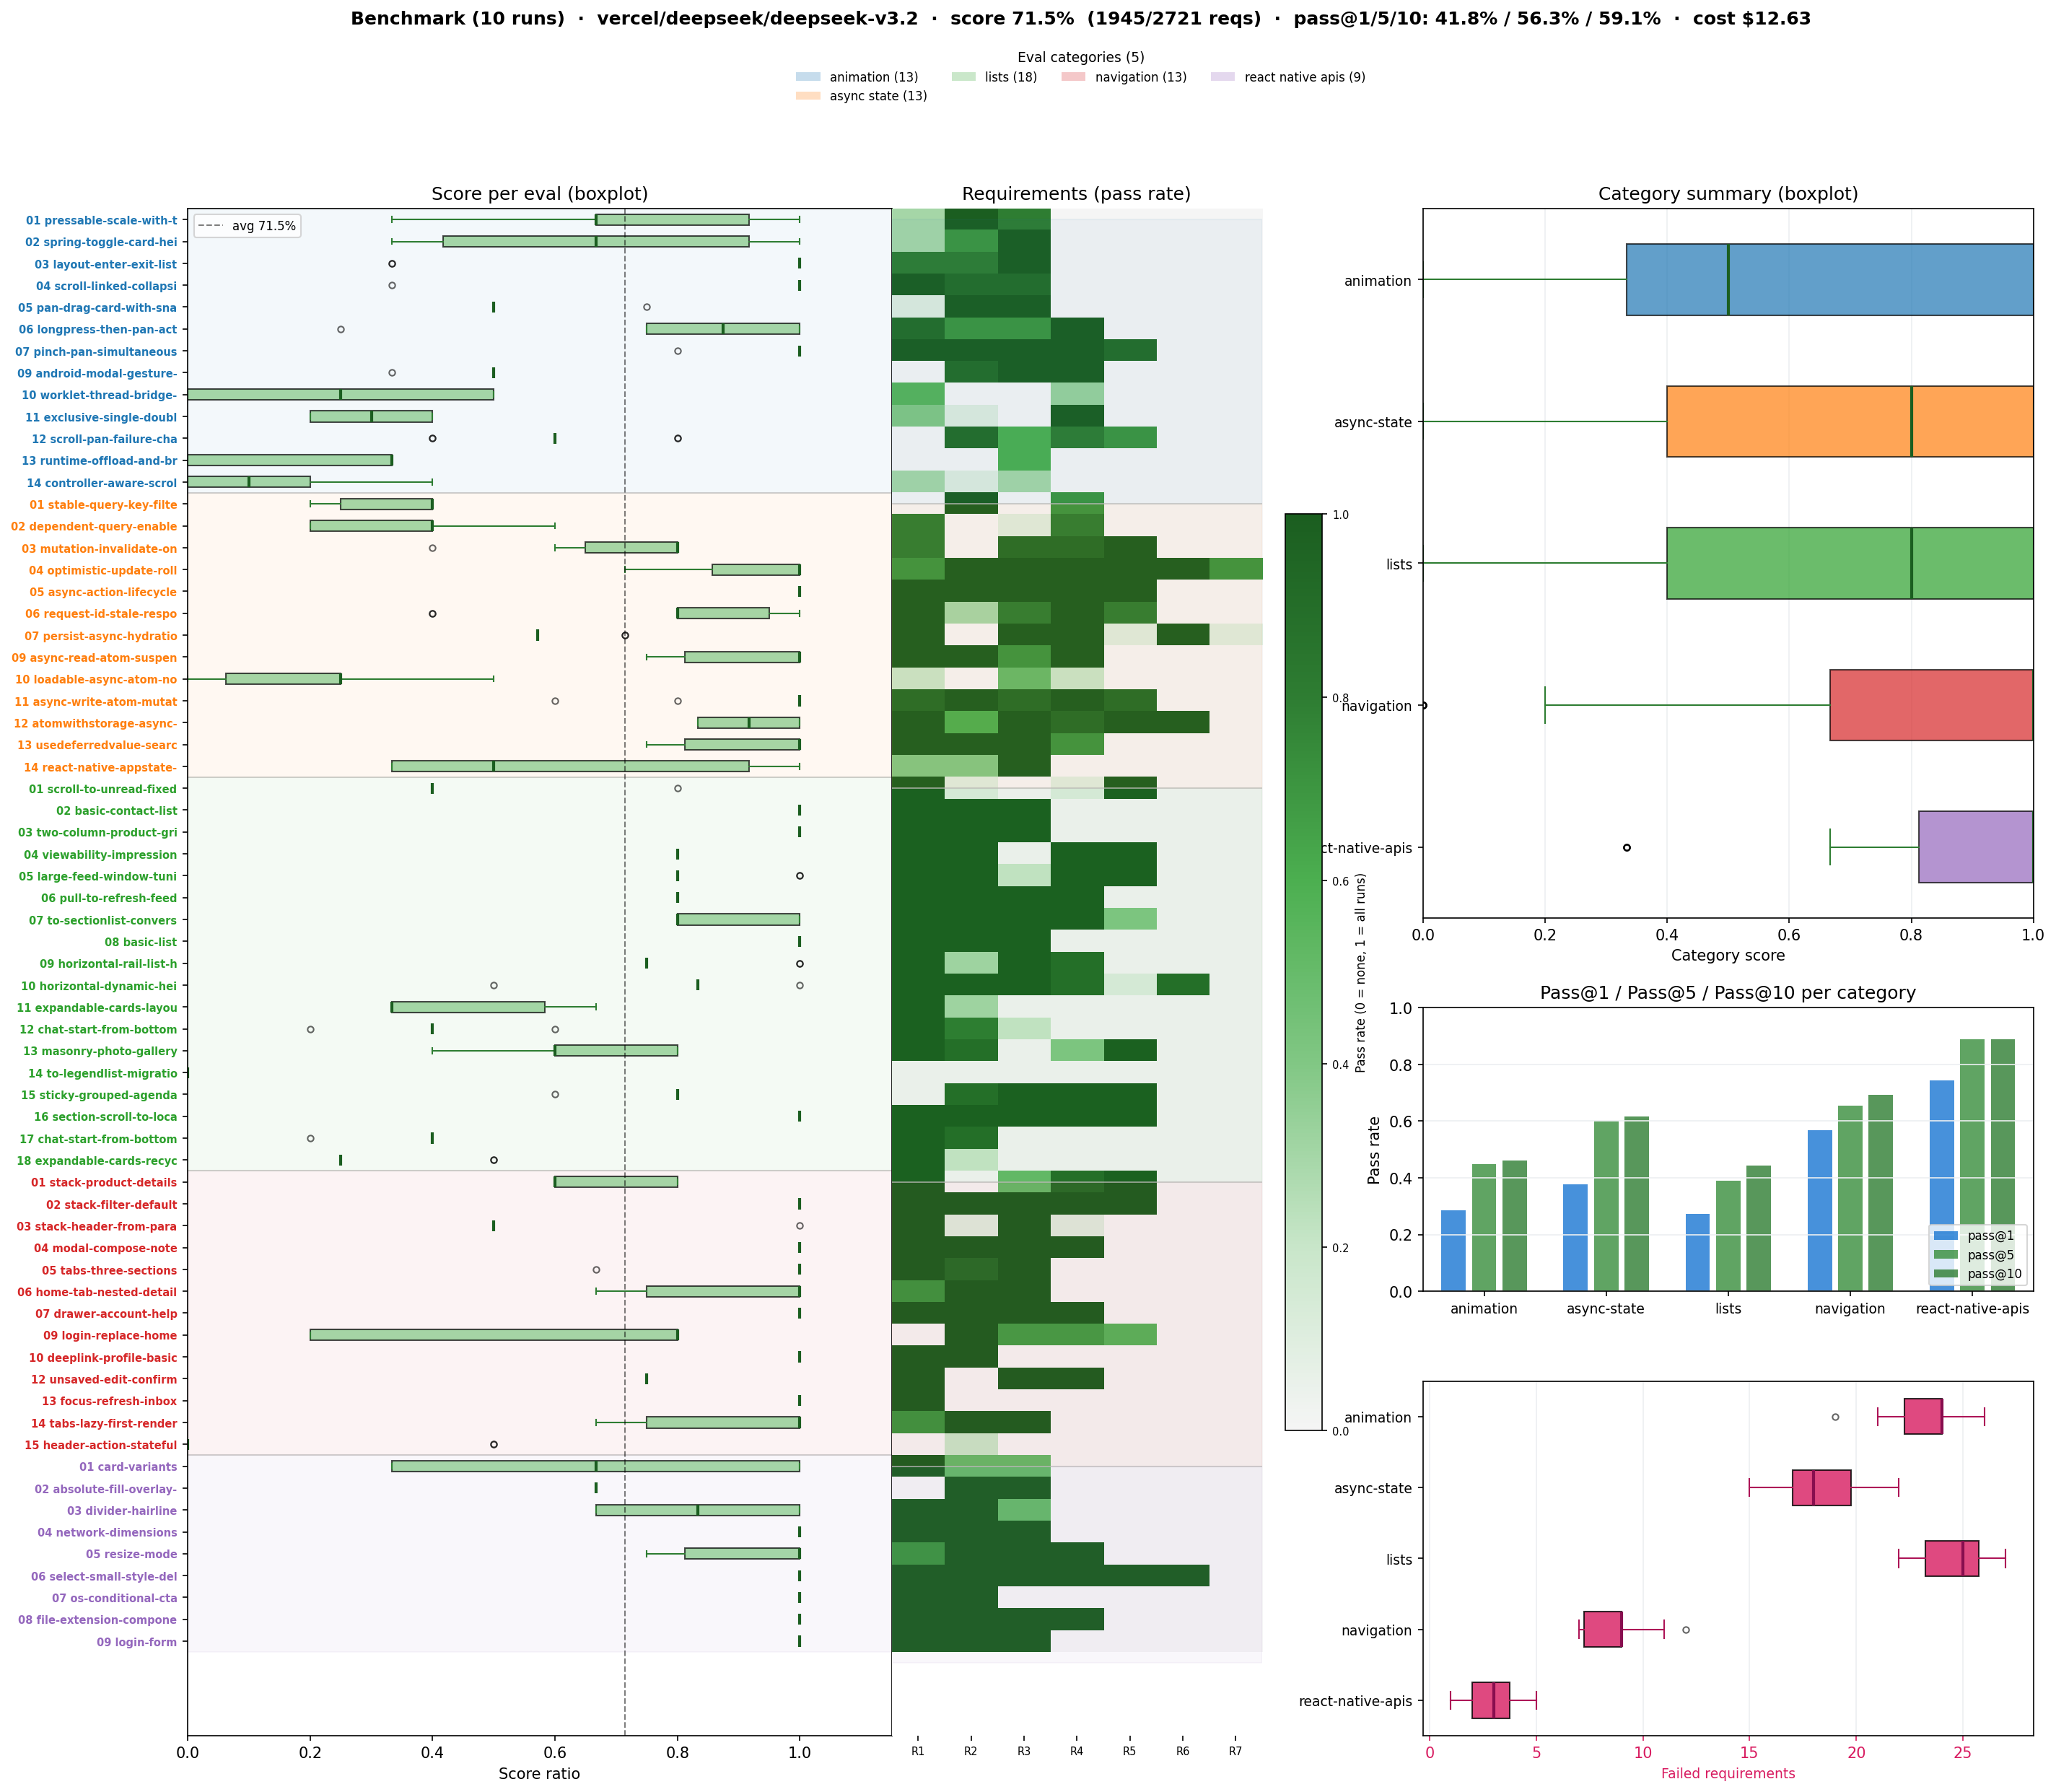
\includegraphics[width=\textwidth]{export/figures/deepseek-v3.2_benchmark_plot.png}
\caption{Benchmark Plot for deepseek-v3.2.}
\end{figure}

\begin{figure}[htbp]
\centering
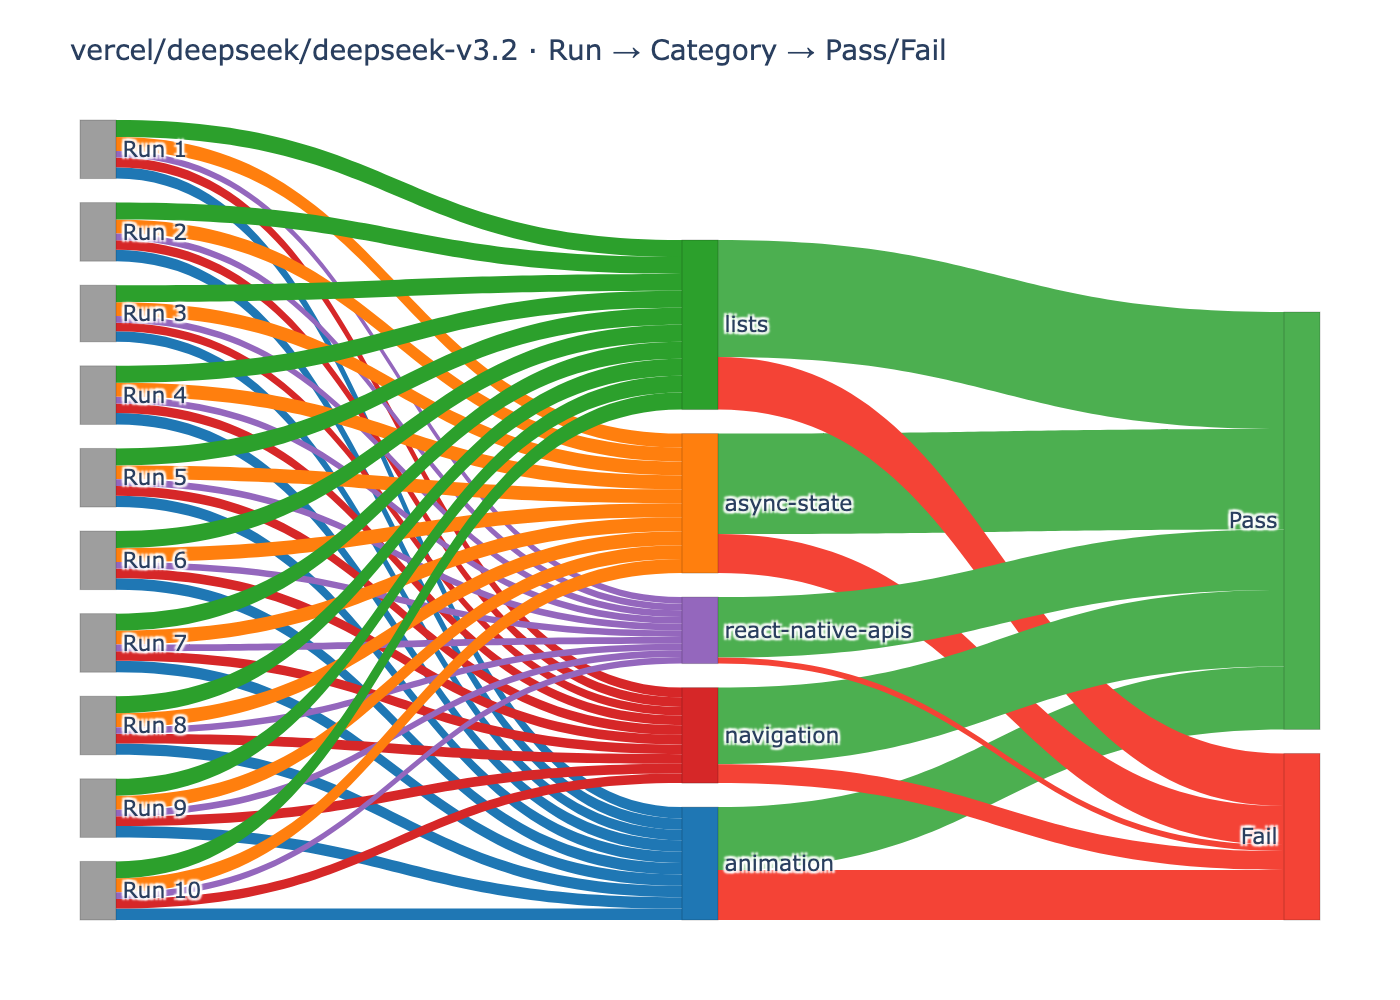
\includegraphics[width=\textwidth]{export/figures/deepseek-v3.2_sankey_per_run.png}
\caption{Sankey per run for deepseek-v3.2 showing the distribution of evals with respect to categories and results}
\end{figure}


\clearpage

\subsection{gemini-3.1-pro-preview}

% Table: summary
% Requires: \usepackage{booktabs}
\begin{table}[htbp]
\centering
\begin{tabular}{lrrrrrr}
\toprule
Model & Runs & Score & Reqs & P@1 & P@5 & P@10 \\
\midrule
vercel/google/gemini-3.1-pro-preview & 10 & 78.9\% & 1286/1630 & 52.3\% & 60.2\% & 64.1\% \\
\bottomrule
\end{tabular}
\caption{Model summary for gemini-3.1-pro-preview}
\end{table}


% Table: category_summary
% Requires: \usepackage{booktabs}
\begin{table}[htbp]
\centering
\begin{tabular}{lrrrr}
\toprule
Category & Score & Evals & Requirements & Failed requirements \\
\midrule
animation & 65.1\% & 130 & 53 & 189 \\
async state & 78.9\% & 130 & 65 & 130 \\
lists & 73.7\% & 180 & 79 & 215 \\
navigation & 95.0\% & 130 & 45 & 25 \\
react native apis & 93.7\% & 90 & 31 & 17 \\
\bottomrule
\end{tabular}
\caption{Results by category for gemini-3.1-pro-preview. Score: mean(per-eval passed/total weight) across evals and runs. Evals: count of evaluation tasks. Requirements: sum of requirement count per eval. Failed requirements: sum of failed requirement instances across runs.}
\end{table}


% Table: per_eval
\input{export/tables/gemini-3.1-pro-preview_per_eval}

\begin{figure}[htbp]
\centering
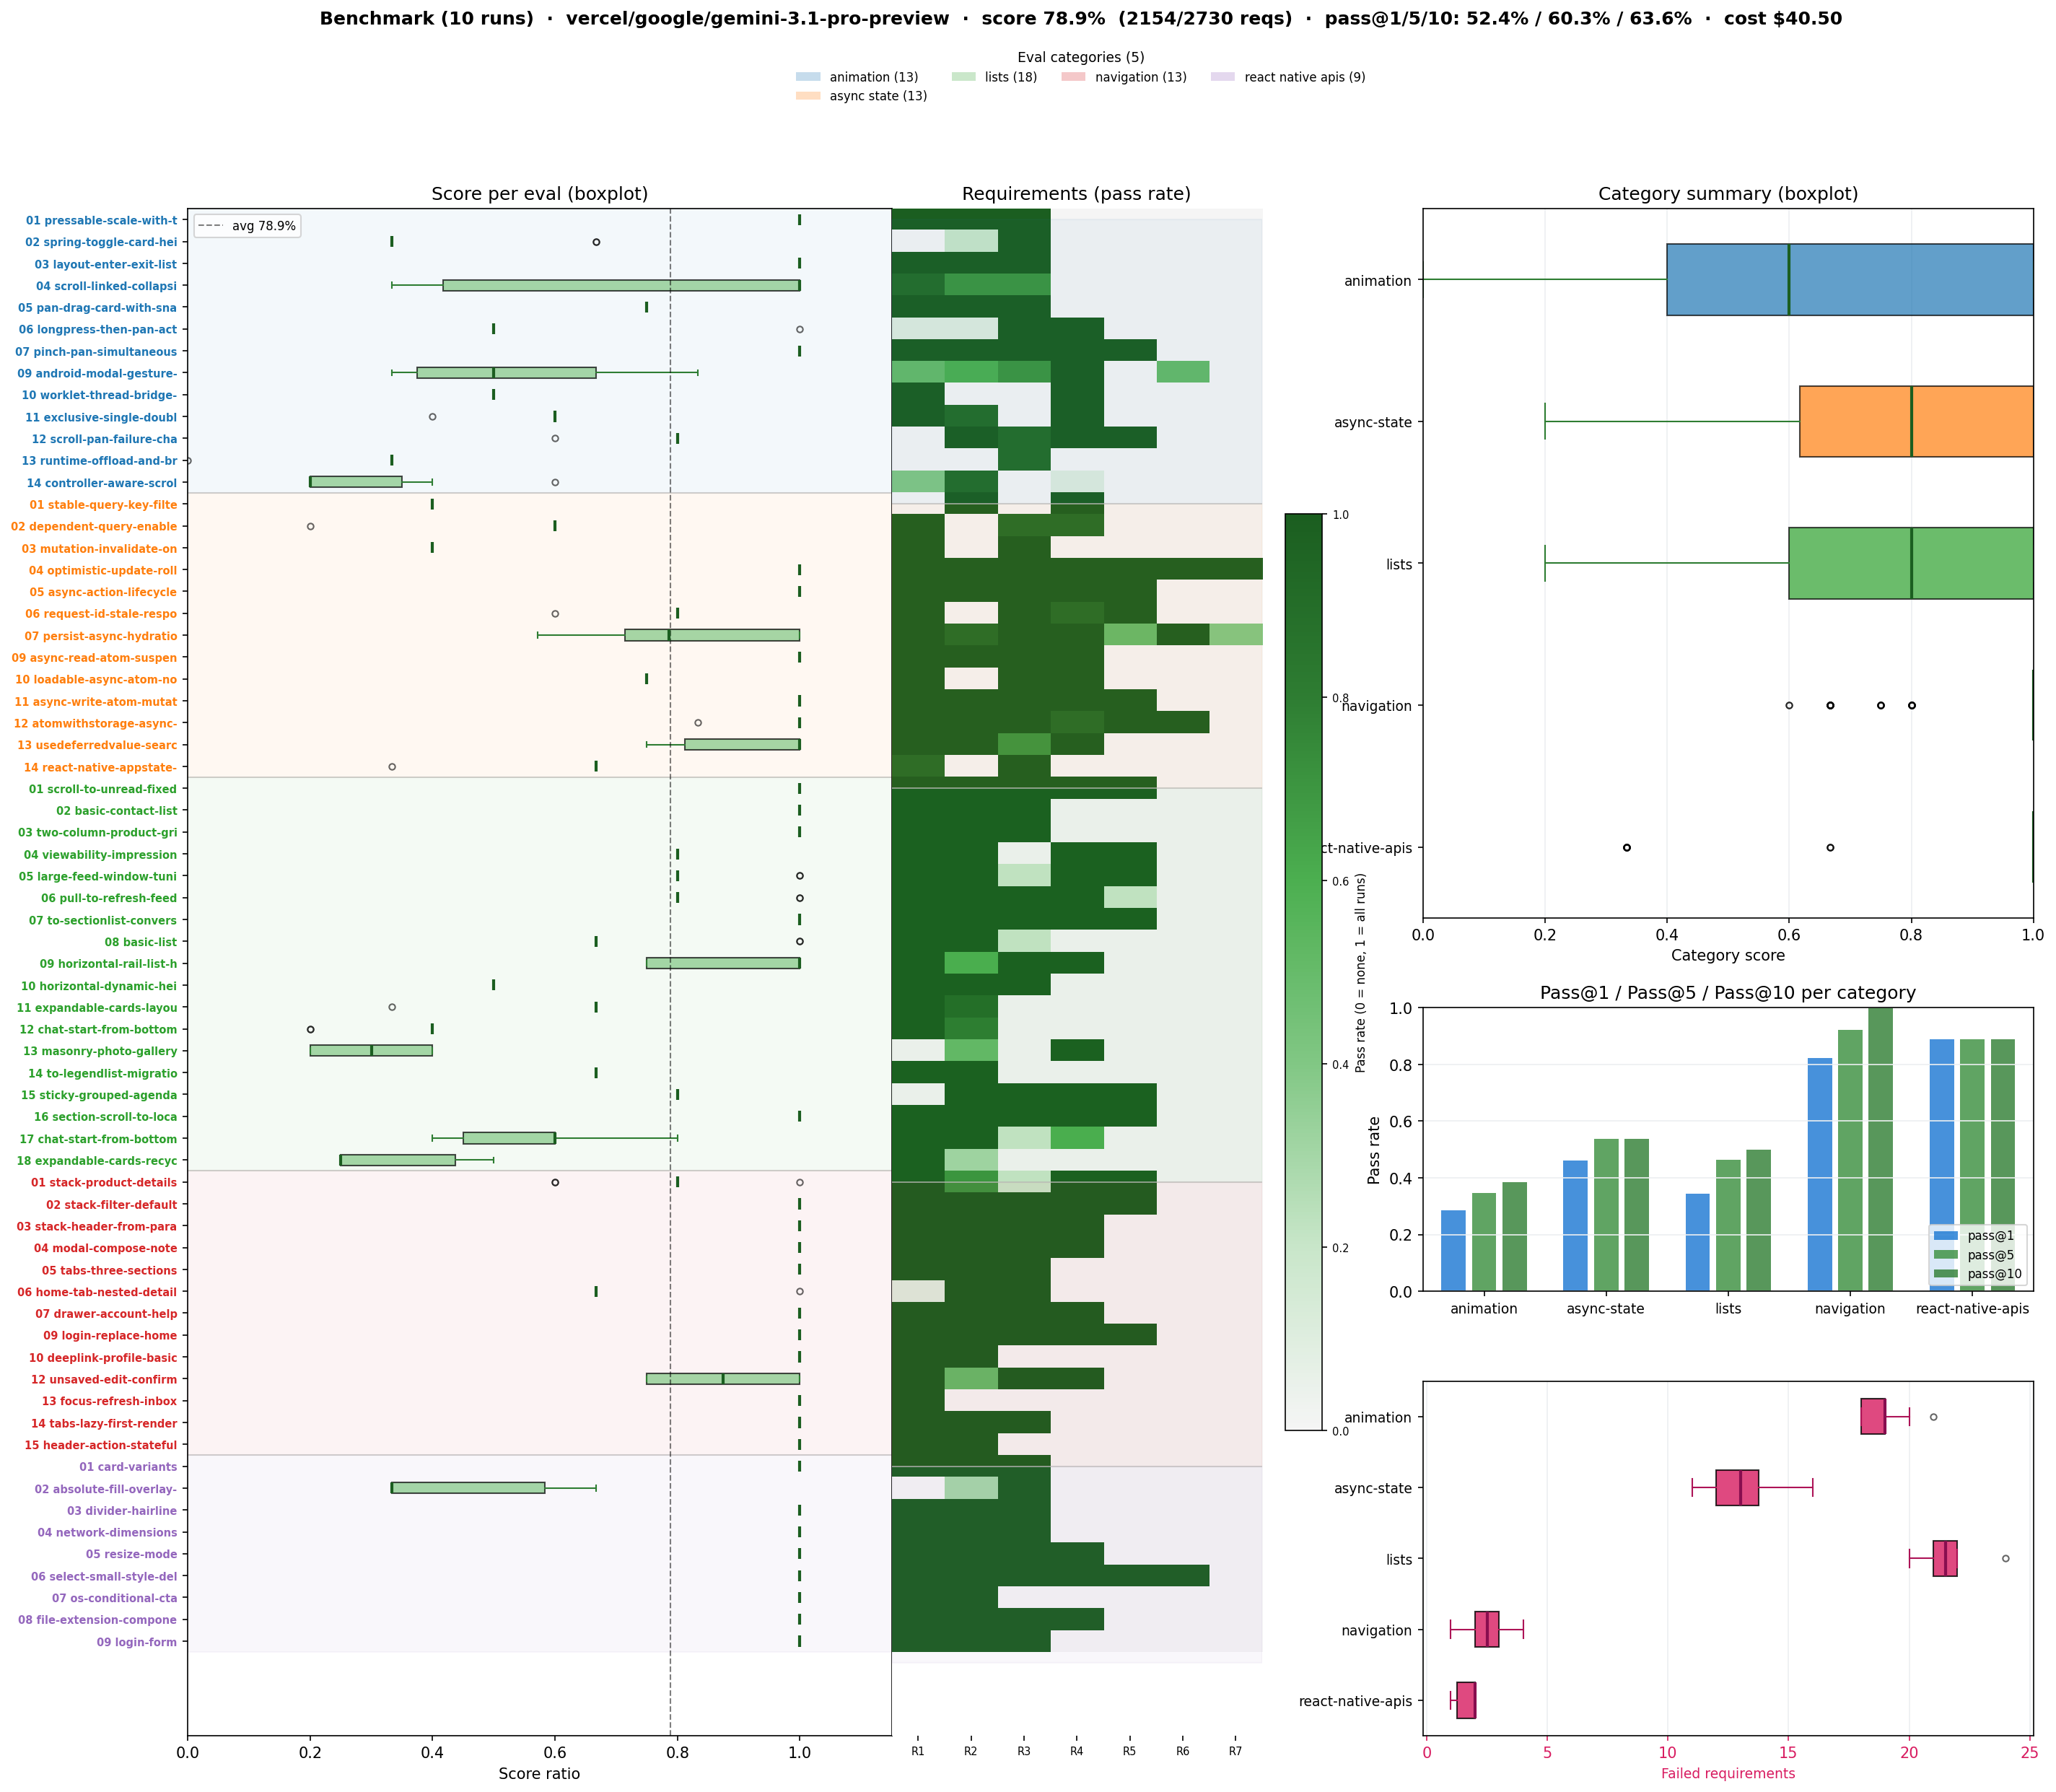
\includegraphics[width=\textwidth]{export/figures/gemini-3.1-pro-preview_benchmark_plot.png}
\caption{Benchmark Plot for gemini-3.1-pro-preview.}
\end{figure}

\begin{figure}[htbp]
\centering
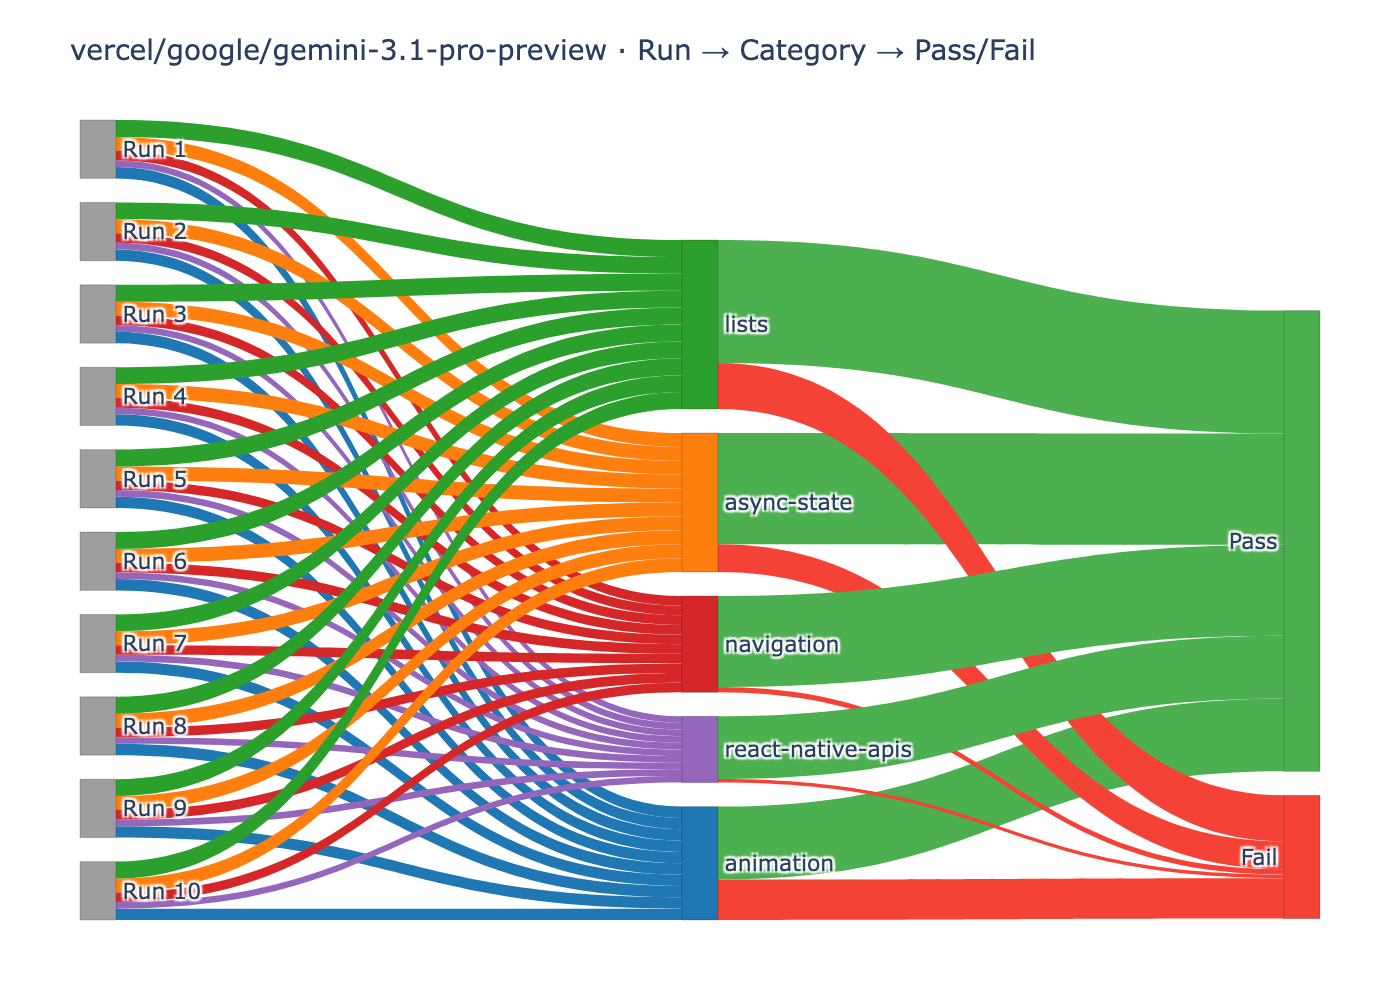
\includegraphics[width=\textwidth]{export/figures/gemini-3.1-pro-preview_sankey_per_run.png}
\caption{Sankey per run for gemini-3.1-pro-preview showing the distribution of evals with respect to categories and results}
\end{figure}


\clearpage

\subsection{glm-5}

% Table: summary
% Requires: \usepackage{booktabs}
\begin{table}[htbp]
\centering
\begin{tabular}{lrrrrrr}
\toprule
Model & Runs & Score & Reqs & P@1 & P@5 & P@10 \\
\midrule
vercel/zai/glm-5 & 10 & 74.2\% & 1210/1630 & 50.8\% & 61.2\% & 61.5\% \\
\bottomrule
\end{tabular}
\caption{Model summary for glm-5}
\end{table}


% Table: category_summary
% Requires: \usepackage{booktabs}
\begin{table}[htbp]
\centering
\begin{tabular}{lrrrr}
\toprule
Category & Score & Evals & Requirements & Failed requirements \\
\midrule
animation & 66.1\% & 130 & 53 & 194 \\
async state & 72.1\% & 130 & 65 & 169 \\
navigation & 89.2\% & 130 & 45 & 57 \\
\bottomrule
\end{tabular}
\caption{Results by category for glm-5. Score: mean(per-eval passed/total weight) across evals and runs. Evals: count of evaluation tasks. Requirements: sum of requirement count per eval. Failed requirements: sum of failed requirement instances across runs.}
\end{table}


% Table: per_eval
% Requires: \usepackage{booktabs}
\begin{table}[htbp]
\centering
\begin{tabular}{lrrrrr}
\toprule
Eval & Category & Score & P@1 & P@5 & P@10 \\
\midrule
01-rn-anim-pressable-scale-with-timing & animation & 100.0\% & 100.0\% & 100.0\% & 100.0\% \\
02-rn-anim-spring-toggle-card-height & animation & 83.3\% & 50.0\% & 99.6\% & 100.0\% \\
03-rn-anim-layout-enter-exit-list-items & animation & 100.0\% & 100.0\% & 100.0\% & 100.0\% \\
04-rn-anim-scroll-linked-collapsing-header & animation & 86.7\% & 70.0\% & 100.0\% & 100.0\% \\
05-rn-anim-pan-drag-card-with-snap-points & animation & 52.5\% & 0.0\% & 0.0\% & 0.0\% \\
06-rn-anim-longpress-then-pan-activation-gate & animation & 82.5\% & 50.0\% & 99.6\% & 100.0\% \\
07-rn-anim-pinch-pan-simultaneous-photo-canvas & animation & 98.0\% & 90.0\% & 100.0\% & 100.0\% \\
09-rn-anim-android-modal-gesture-root-safety & animation & 46.7\% & 0.0\% & 0.0\% & 0.0\% \\
10-rn-anim-worklet-thread-bridge-schedule-on-rn & animation & 50.0\% & 0.0\% & 0.0\% & 0.0\% \\
11-rn-rngh-exclusive-single-double-tap & animation & 40.0\% & 0.0\% & 0.0\% & 0.0\% \\
12-rn-rngh-scroll-pan-failure-chain & animation & 74.0\% & 0.0\% & 0.0\% & 0.0\% \\
13-rn-worklets-runtime-offload-and-bridge & animation & 30.0\% & 0.0\% & 0.0\% & 0.0\% \\
14-rn-keyboard-controller-aware-scroll-footer & animation & 16.0\% & 0.0\% & 0.0\% & 0.0\% \\
01-rn-rq-stable-query-key-filters & async state & 40.0\% & 0.0\% & 0.0\% & 0.0\% \\
02-rn-rq-dependent-query-enabled-gate & async state & 42.0\% & 0.0\% & 0.0\% & 0.0\% \\
03-rn-rq-mutation-invalidate-on-success & async state & 58.0\% & 0.0\% & 0.0\% & 0.0\% \\
04-rn-rq-optimistic-update-rollback & async state & 98.6\% & 90.0\% & 100.0\% & 100.0\% \\
05-rn-zustand-async-action-lifecycle & async state & 100.0\% & 100.0\% & 100.0\% & 100.0\% \\
06-rn-zustand-request-id-stale-response-guard & async state & 68.0\% & 30.0\% & 91.7\% & 100.0\% \\
07-rn-zustand-persist-async-hydration-gate & async state & 64.3\% & 0.0\% & 0.0\% & 0.0\% \\
09-rn-jotai-async-read-atom-suspense & async state & 100.0\% & 100.0\% & 100.0\% & 100.0\% \\
10-rn-jotai-loadable-async-atom-no-suspense & async state & 40.0\% & 0.0\% & 0.0\% & 0.0\% \\
11-rn-jotai-async-write-atom-mutation & async state & 100.0\% & 100.0\% & 100.0\% & 100.0\% \\
12-rn-jotai-atomwithstorage-async-rehydrate-guard & async state & 98.3\% & 90.0\% & 100.0\% & 100.0\% \\
13-rn-react-usedeferredvalue-search-stale-indicator & async state & 95.0\% & 80.0\% & 100.0\% & 100.0\% \\
14-rn-rq-react-native-appstate-focus-online-managers & async state & 33.3\% & 0.0\% & 0.0\% & 0.0\% \\
01-rn-nav-stack-product-details & navigation & 66.0\% & 0.0\% & 0.0\% & 0.0\% \\
02-rn-nav-stack-filter-default & navigation & 100.0\% & 100.0\% & 100.0\% & 100.0\% \\
03-rn-nav-stack-header-from-param & navigation & 100.0\% & 100.0\% & 100.0\% & 100.0\% \\
04-rn-nav-modal-compose-note & navigation & 100.0\% & 100.0\% & 100.0\% & 100.0\% \\
05-rn-nav-tabs-three-sections & navigation & 100.0\% & 100.0\% & 100.0\% & 100.0\% \\
06-rn-nav-home-tab-nested-details & navigation & 80.0\% & 40.0\% & 97.6\% & 100.0\% \\
07-rn-nav-drawer-account-help & navigation & 97.5\% & 90.0\% & 100.0\% & 100.0\% \\
09-rn-nav-login-replace-home & navigation & 58.0\% & 0.0\% & 0.0\% & 0.0\% \\
10-rn-nav-deeplink-profile-basic & navigation & 100.0\% & 100.0\% & 100.0\% & 100.0\% \\
12-rn-nav-unsaved-edit-confirm & navigation & 82.5\% & 40.0\% & 97.6\% & 100.0\% \\
13-rn-nav-focus-refresh-inbox & navigation & 100.0\% & 100.0\% & 100.0\% & 100.0\% \\
14-rn-nav-tabs-lazy-first-render & navigation & 100.0\% & 100.0\% & 100.0\% & 100.0\% \\
15-rn-nav-header-action-stateful & navigation & 75.0\% & 60.0\% & 100.0\% & 100.0\% \\
\bottomrule
\end{tabular}
\caption{Per-eval results (score and pass@k) for glm-5}
\end{table}


\begin{figure}[htbp]
\centering
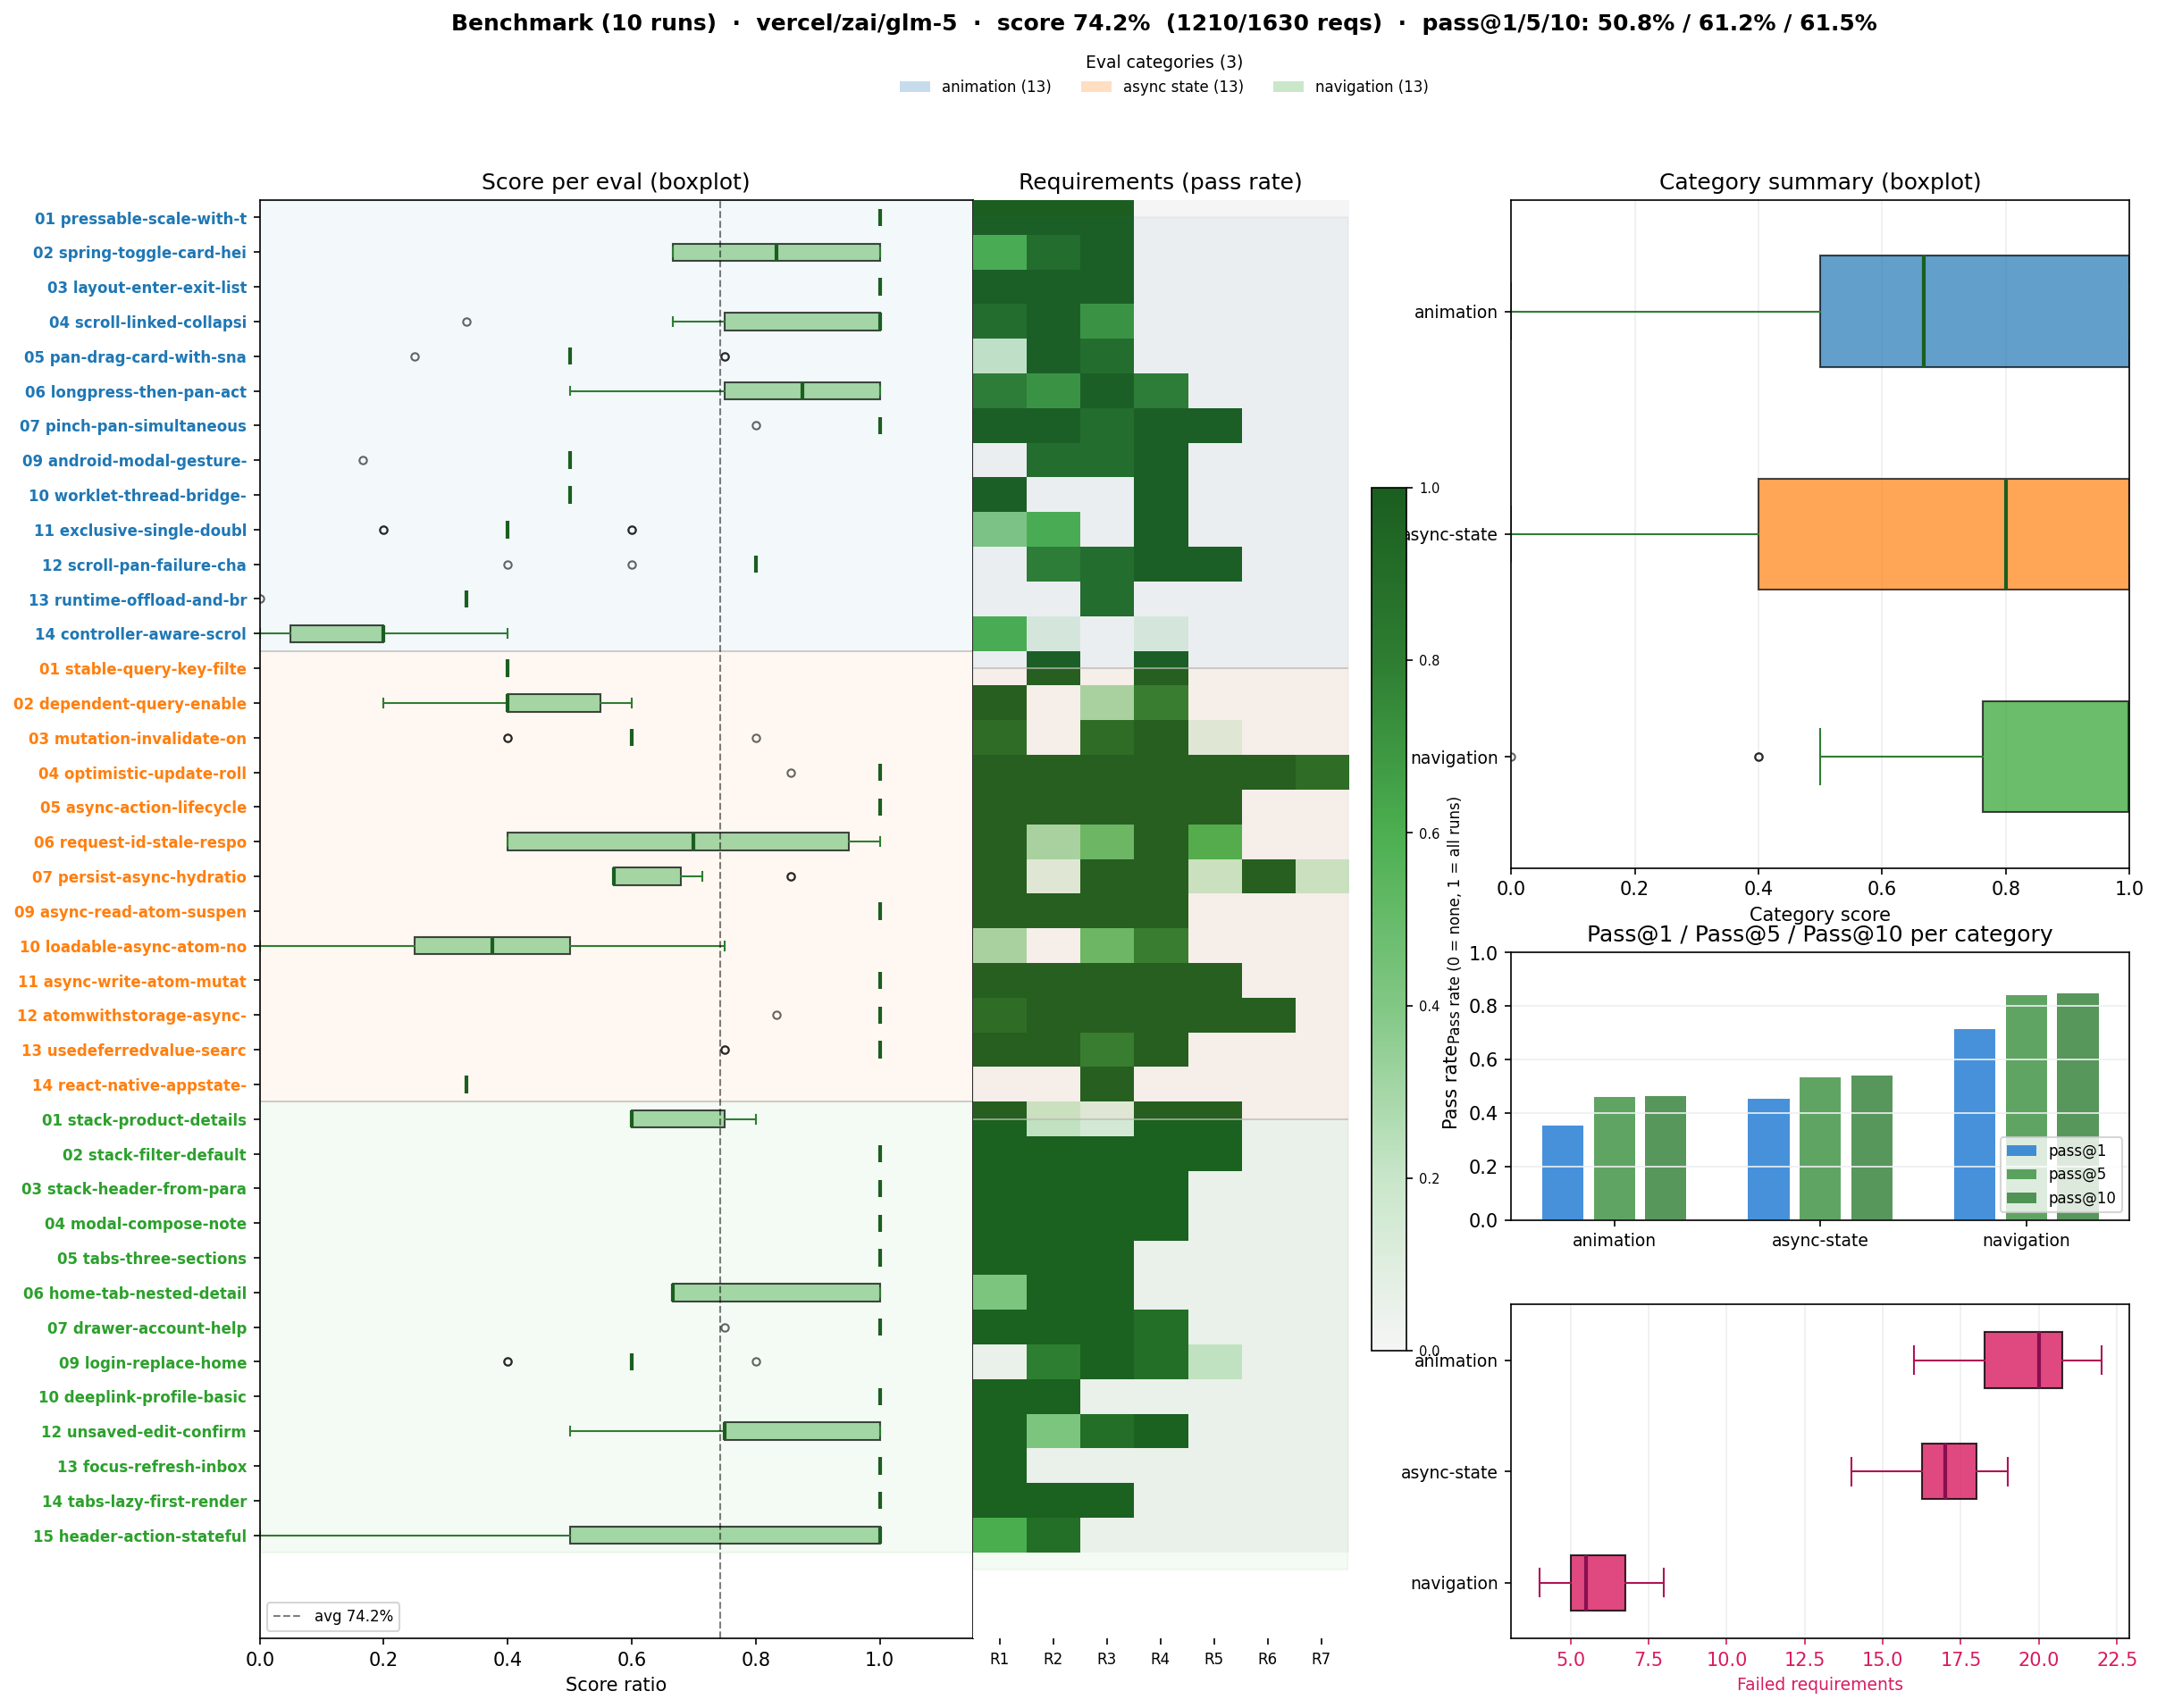
\includegraphics[width=\textwidth]{export/figures/glm-5_benchmark_plot.png}
\caption{Benchmark Plot for glm-5.}
\end{figure}

\begin{figure}[htbp]
\centering
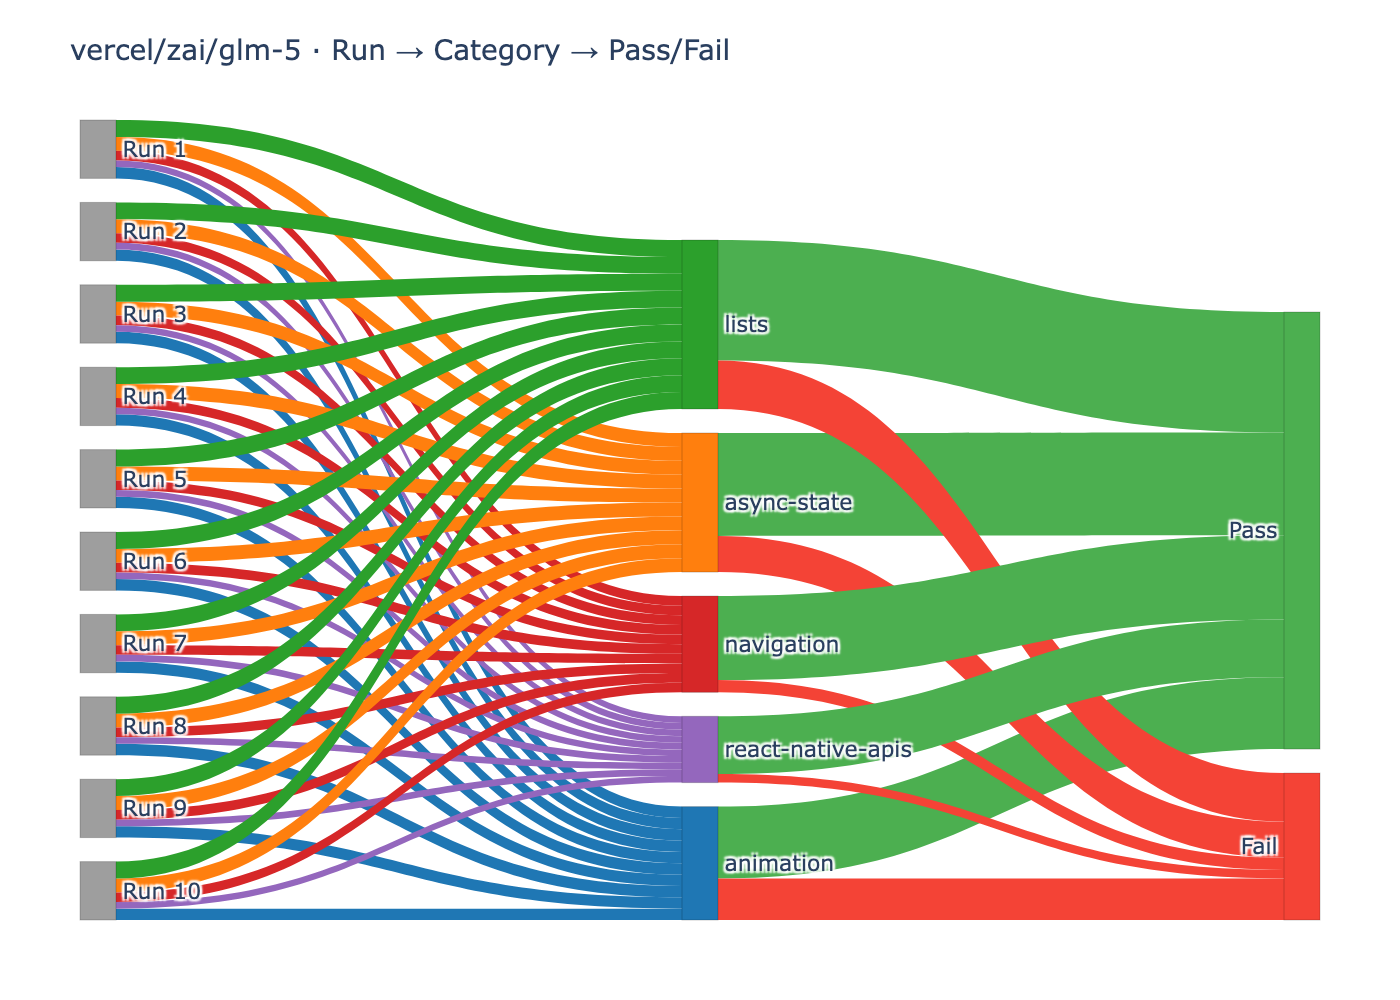
\includegraphics[width=\textwidth]{export/figures/glm-5_sankey_per_run.png}
\caption{Sankey per run for glm-5 showing the distribution of evals with respect to categories and results}
\end{figure}


\clearpage

\subsection{gpt-5.3-codex}

% Table: summary
% Requires: \usepackage{booktabs}
\begin{table}[htbp]
\centering
\begin{tabular}{lrrrrrr}
\toprule
Model & Runs & Score & Reqs & P@1 & P@5 & P@10 \\
\midrule
vercel/openai/gpt-5.3-codex & 10 & 83.1\% & 2267/2727 & 63.3\% & 74.5\% & 78.5\% \\
\bottomrule
\end{tabular}
\caption{Model summary for gpt-5.3-codex}
\end{table}


% Table: category_summary
% Requires: \usepackage{booktabs}
\begin{table}[htbp]
\centering
\begin{tabular}{lrrrr}
\toprule
Category & Score & Evals & Requirements & Failed requirements \\
\midrule
animation & 67.1\% & 130 & 53 & 186 \\
async state & 83.4\% & 129 & 65 & 105 \\
navigation & 96.2\% & 130 & 45 & 20 \\
\bottomrule
\end{tabular}
\caption{Results by category for gpt-5.3-codex. Score: mean(per-eval passed/total weight) across evals and runs. Evals: count of evaluation tasks. Requirements: sum of requirement count per eval. Failed requirements: sum of failed requirement instances across runs.}
\end{table}


% Table: per_eval
\input{export/tables/gpt-5.3-codex_per_eval}

\begin{figure}[htbp]
\centering
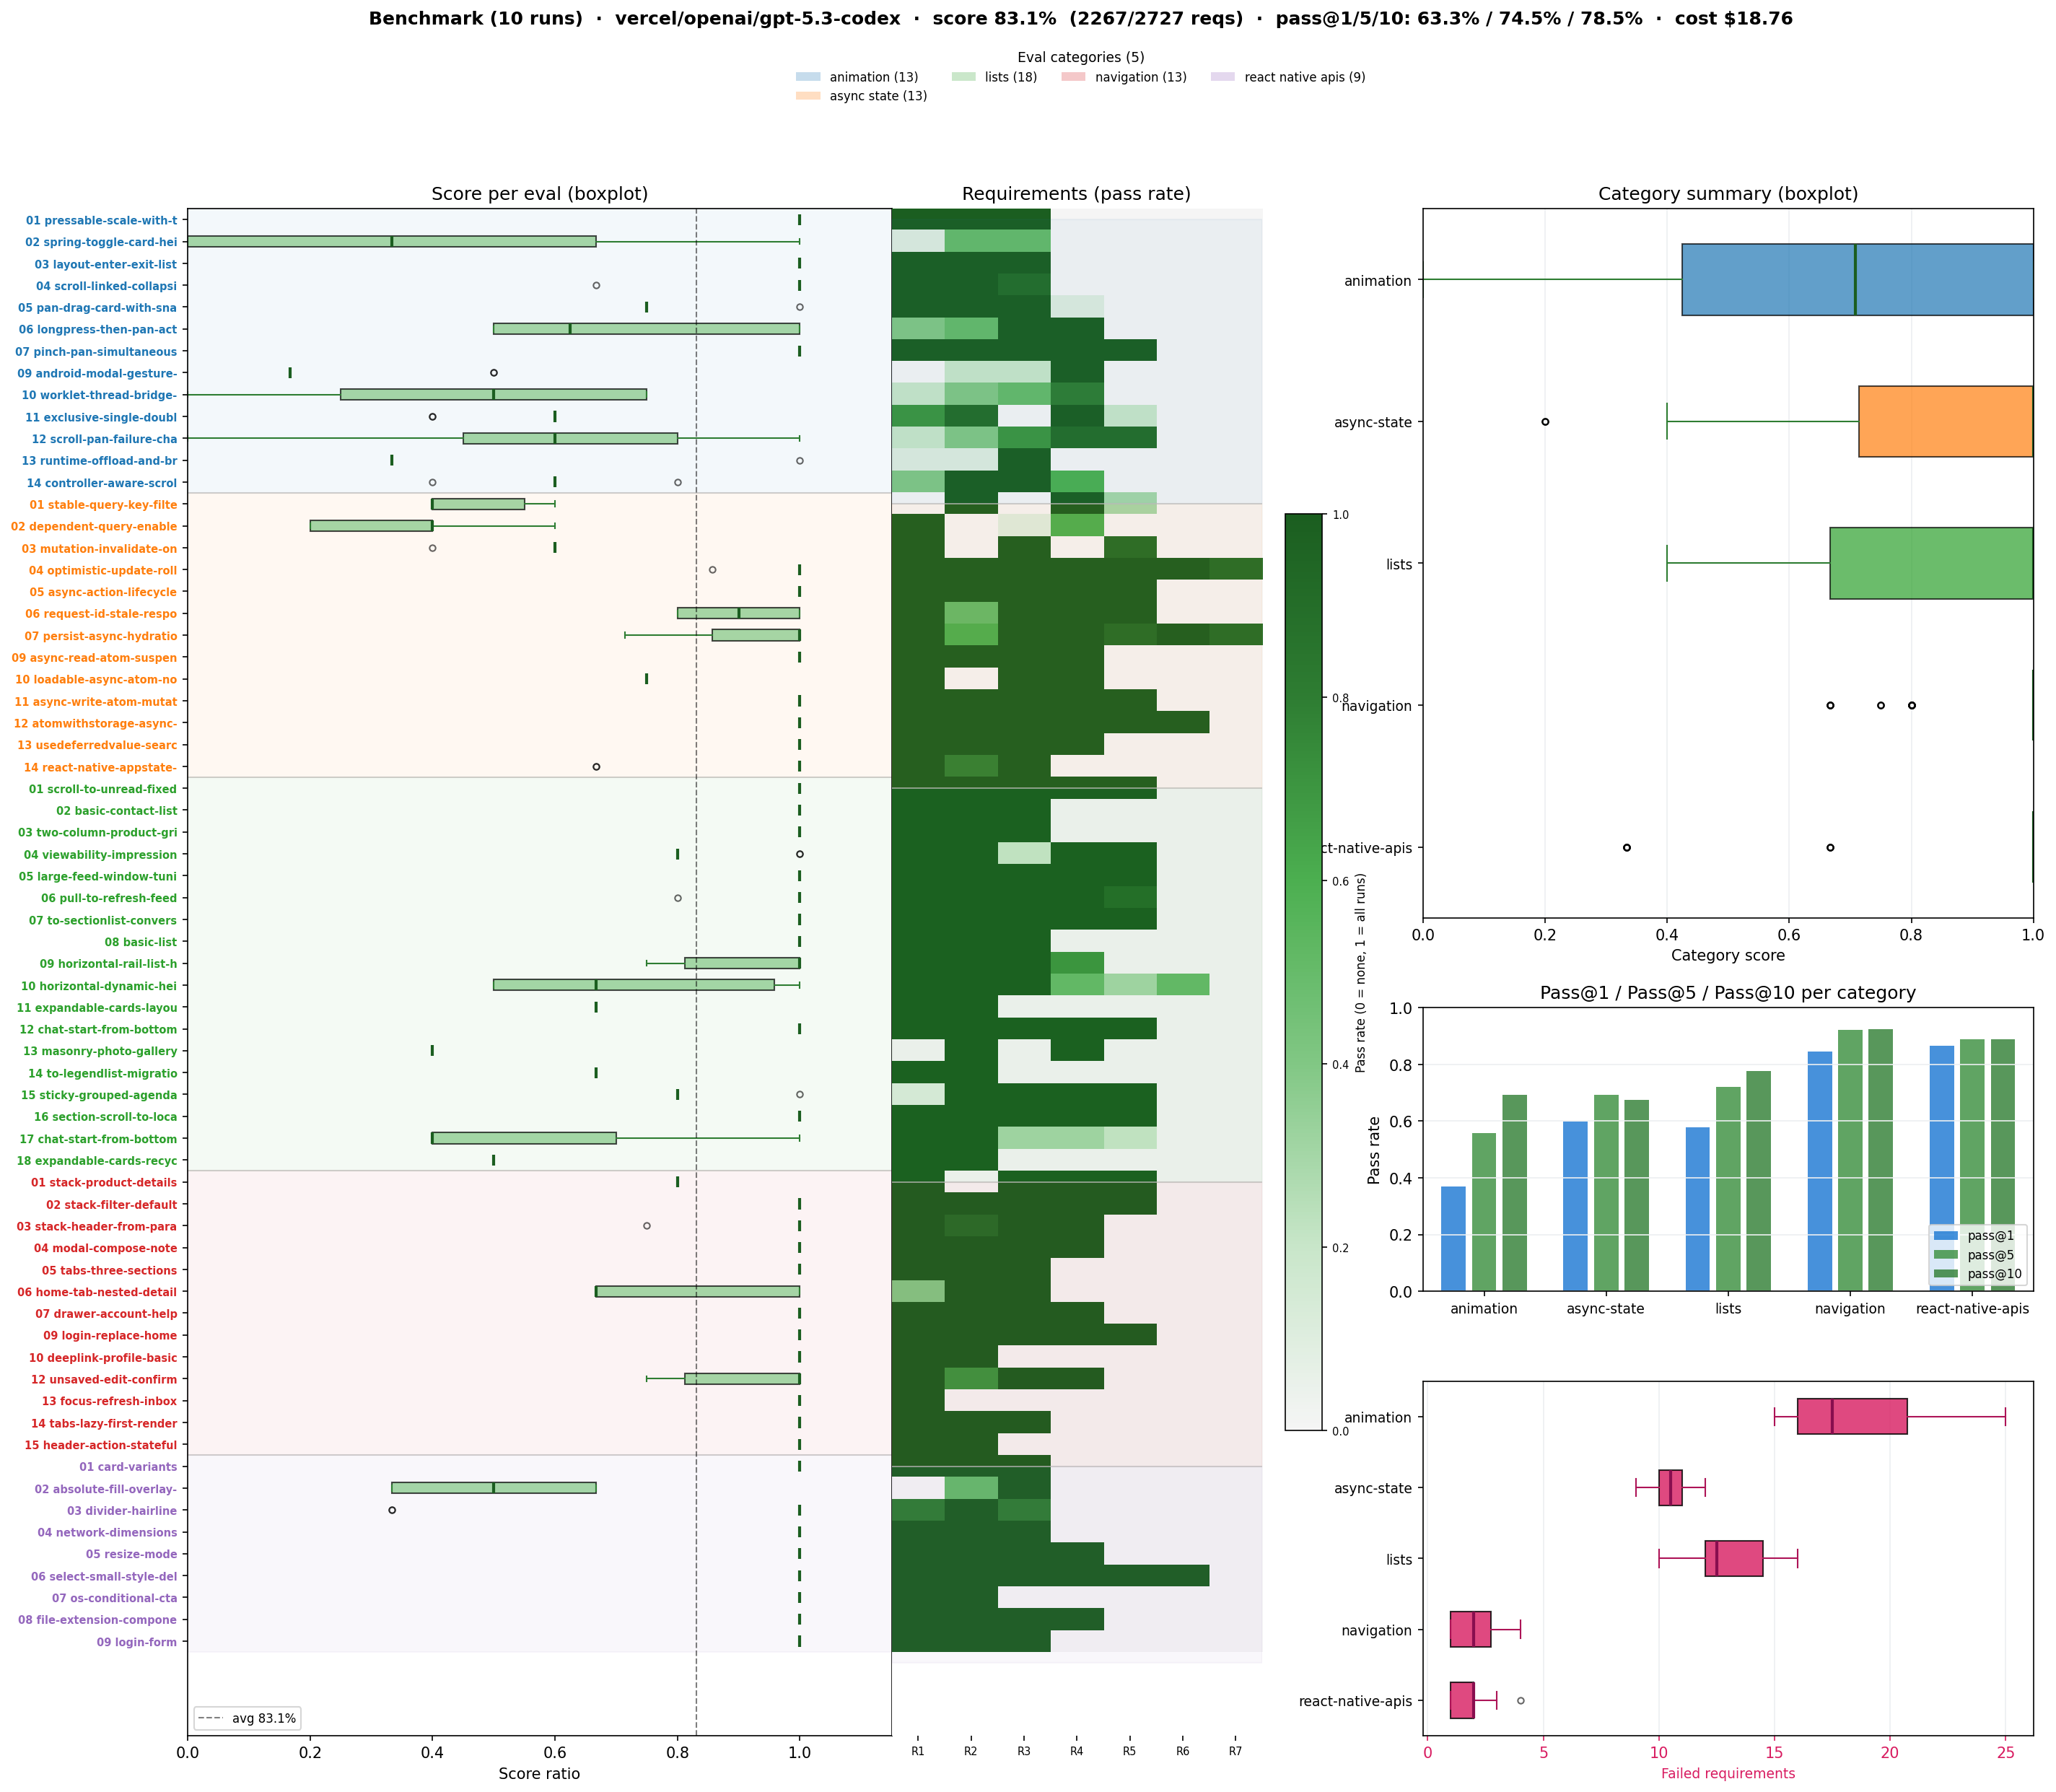
\includegraphics[width=\textwidth]{export/figures/gpt-5.3-codex_benchmark_plot.png}
\caption{Benchmark Plot for gpt-5.3-codex.}
\end{figure}

\begin{figure}[htbp]
\centering
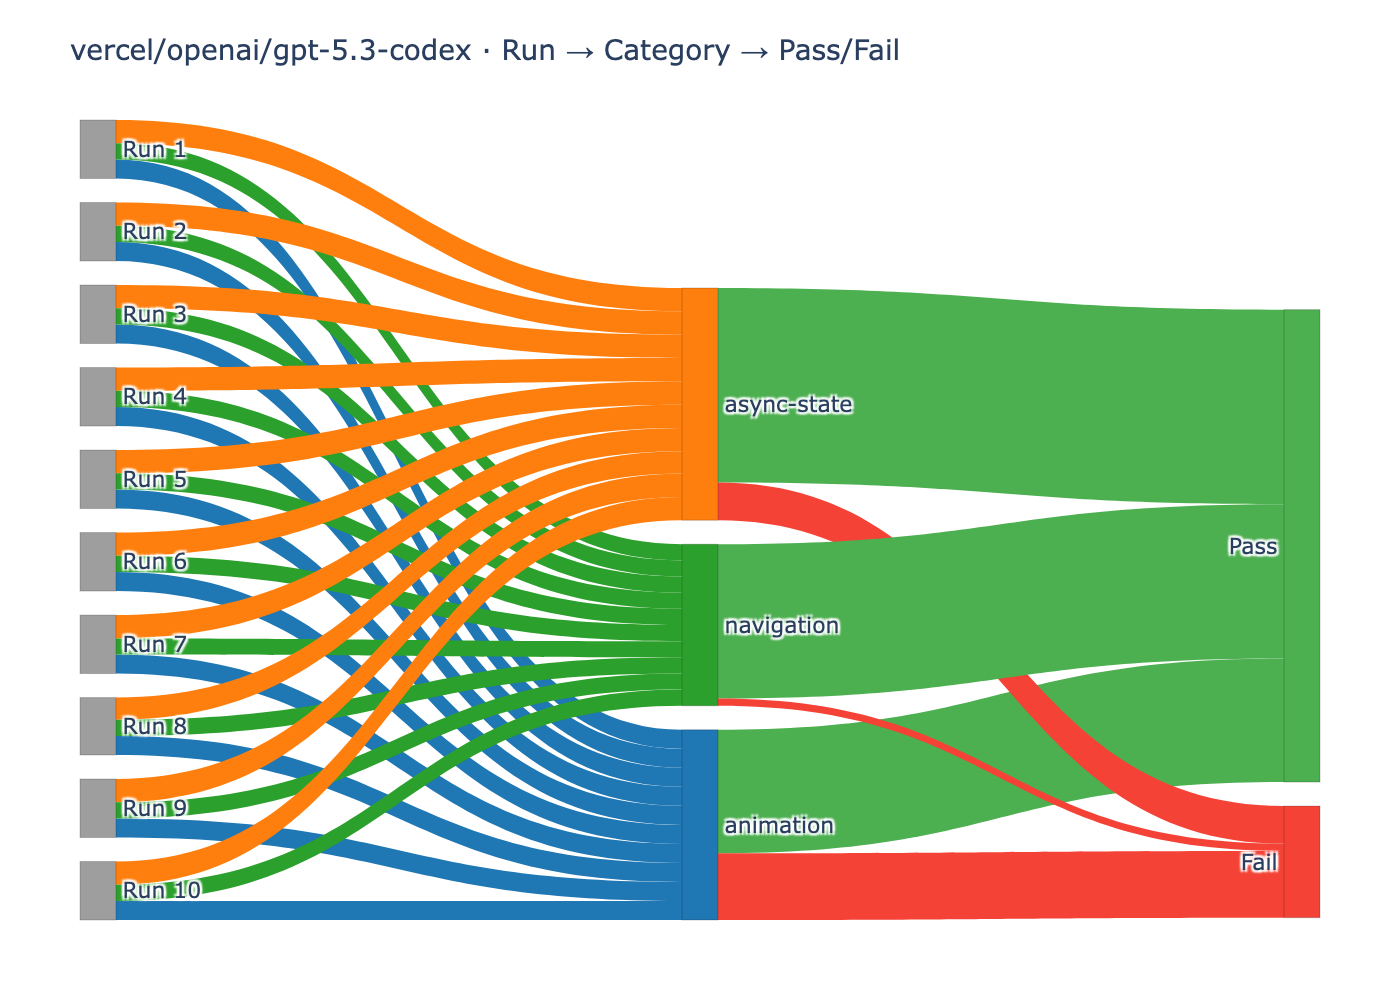
\includegraphics[width=\textwidth]{export/figures/gpt-5.3-codex_sankey_per_run.png}
\caption{Sankey per run for gpt-5.3-codex showing the distribution of evals with respect to categories and results}
\end{figure}


\clearpage

\subsection{gpt-5.4}

% Table: summary
% Requires: \usepackage{booktabs}
\begin{table}[htbp]
\centering
\begin{tabular}{lrrrrrr}
\toprule
Model & Runs & Score & Reqs & P@1 & P@5 & P@10 \\
\midrule
vercel/openai/gpt-5.4 & 10 & 85.3\% & 2330/2730 & 64.4\% & 74.7\% & 75.8\% \\
\bottomrule
\end{tabular}
\caption{Model summary for gpt-5.4}
\end{table}


% Table: category_summary
% Requires: \usepackage{booktabs}
\begin{table}[htbp]
\centering
\begin{tabular}{lrrrr}
\toprule
Category & Score & Evals & Requirements & Failed requirements \\
\midrule
animation & 71.3\% & 130 & 53 & 164 \\
async state & 85.6\% & 130 & 65 & 96 \\
navigation & 95.1\% & 130 & 45 & 23 \\
\bottomrule
\end{tabular}
\caption{Results by category for gpt-5.4. Score: mean(per-eval passed/total weight) across evals and runs. Evals: count of evaluation tasks. Requirements: sum of requirement count per eval. Failed requirements: sum of failed requirement instances across runs.}
\end{table}


% Table: per_eval
\input{export/tables/gpt-5.4_per_eval}

\begin{figure}[htbp]
\centering
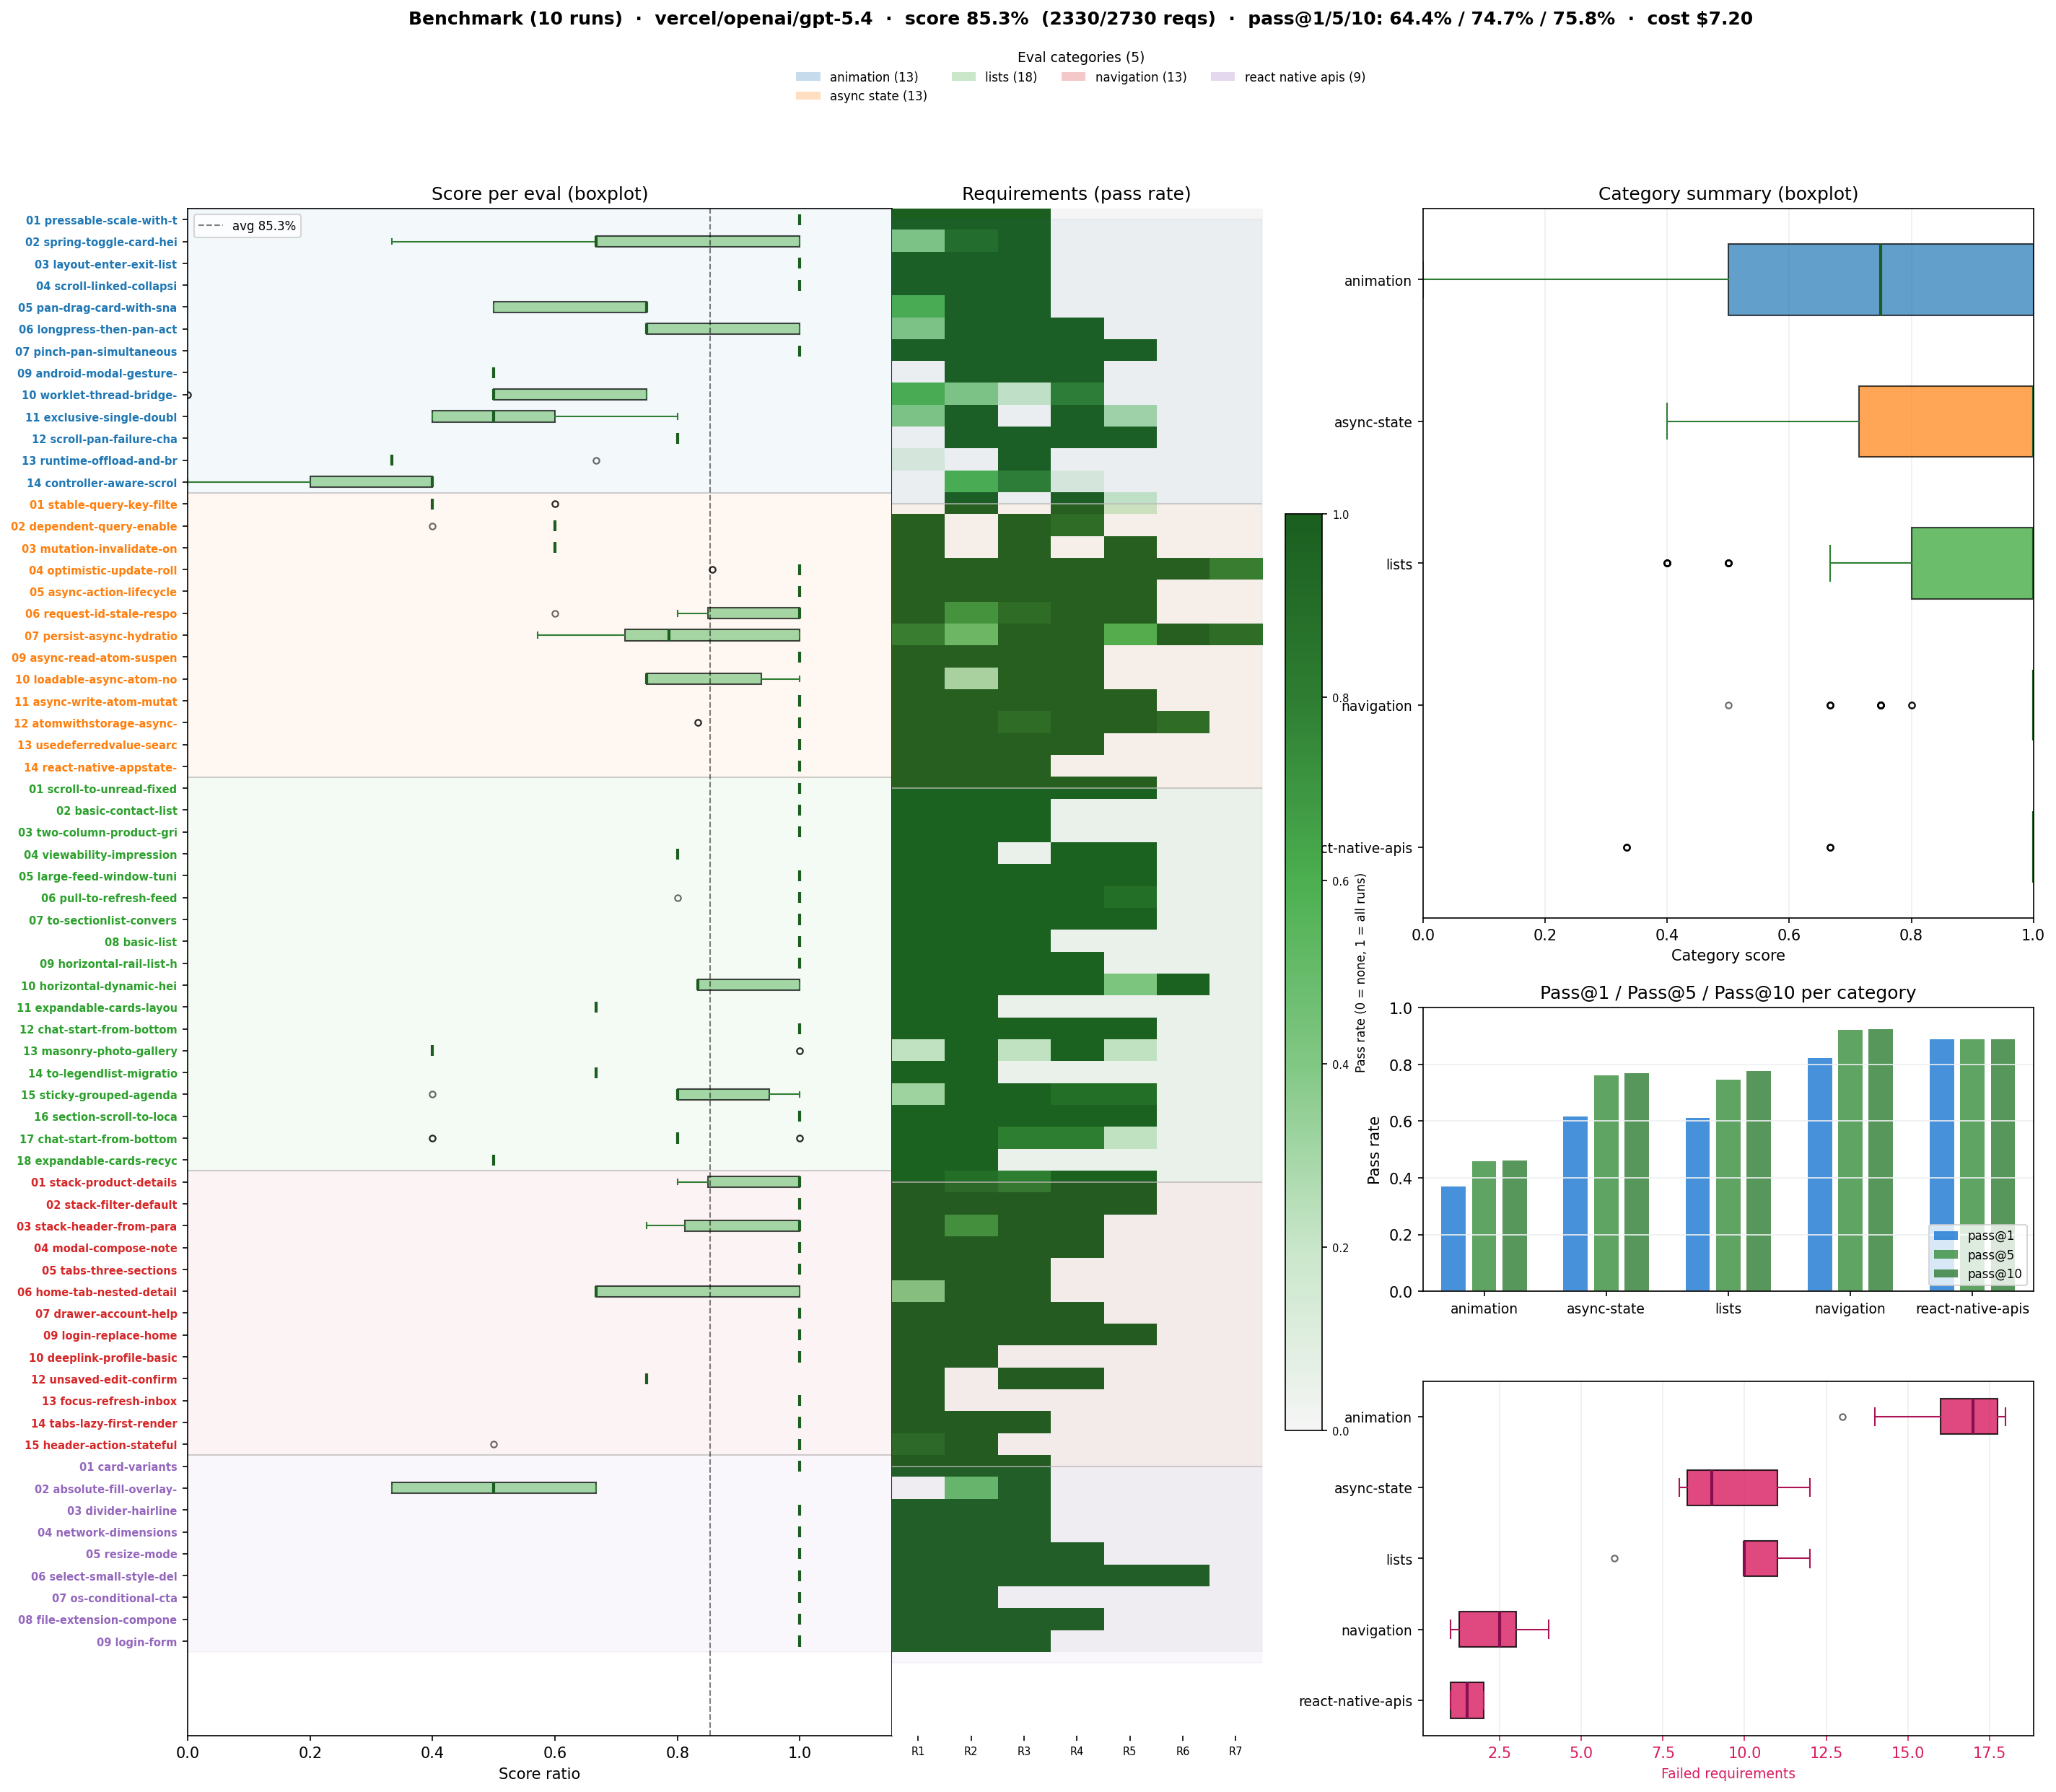
\includegraphics[width=\textwidth]{export/figures/gpt-5.4_benchmark_plot.png}
\caption{Benchmark Plot for gpt-5.4.}
\end{figure}

\begin{figure}[htbp]
\centering
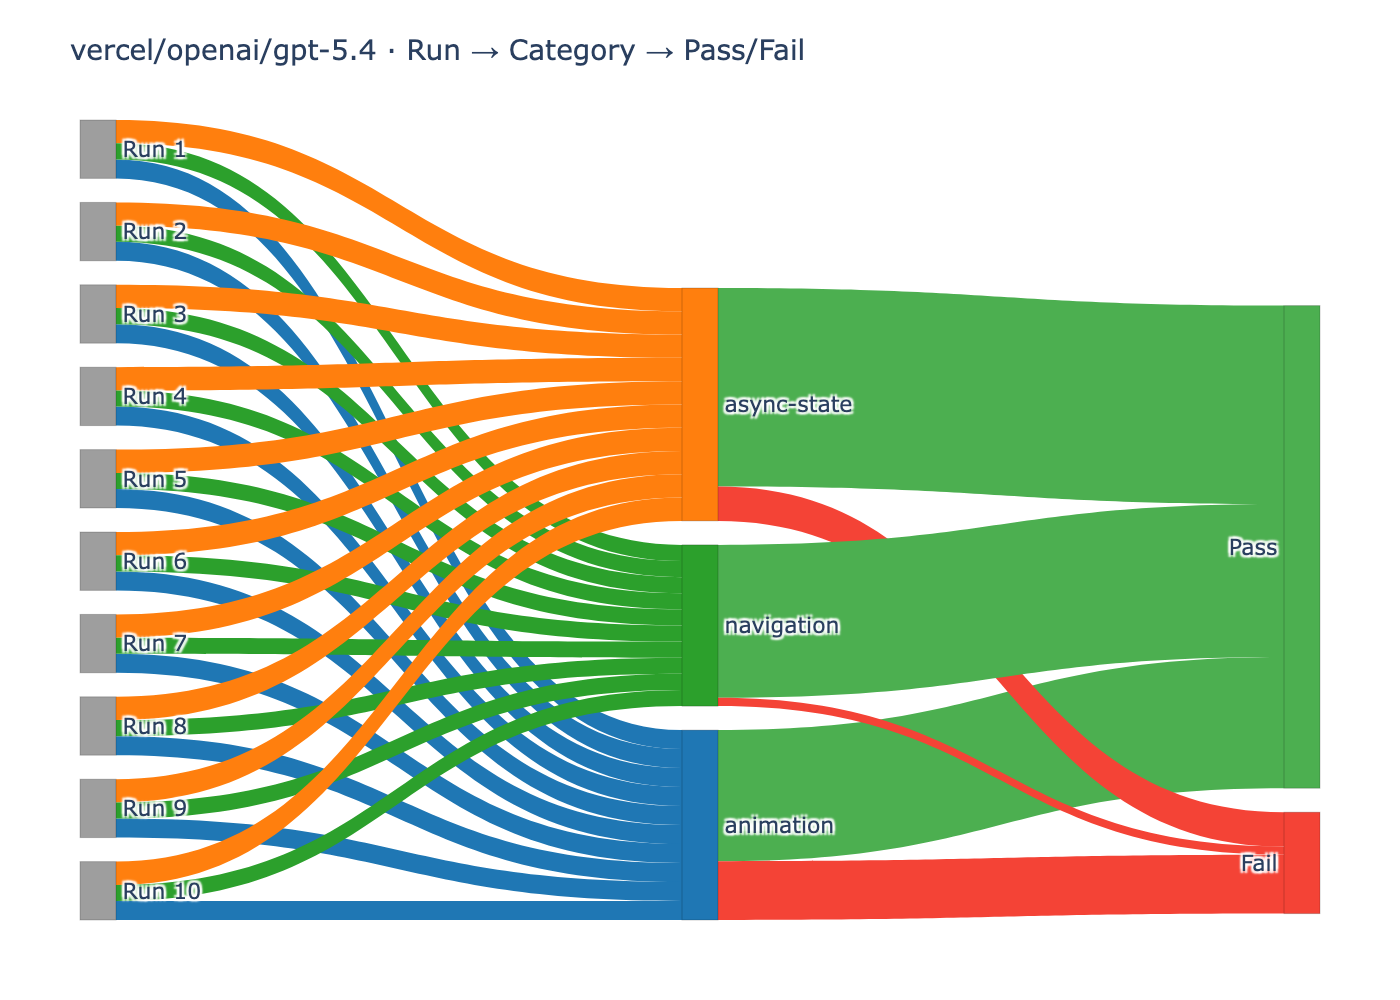
\includegraphics[width=\textwidth]{export/figures/gpt-5.4_sankey_per_run.png}
\caption{Sankey per run for gpt-5.4 showing the distribution of evals with respect to categories and results}
\end{figure}


\clearpage

\subsection{gpt-oss-120b}

% Table: summary
% Requires: \usepackage{booktabs}
\begin{table}[htbp]
\centering
\begin{tabular}{lrrrrrr}
\toprule
Model & Runs & Score & Reqs & P@1 & P@5 & P@10 \\
\midrule
cloudflare-ai-gateway/workers-ai/@cf/openai/gpt-os & 10 & 71.6\% & 1653/2308 & 46.0\% & 54.3\% & 50.4\% \\
\bottomrule
\end{tabular}
\caption{Model summary for gpt-oss-120b}
\end{table}


% Table: category_summary
% Requires: \usepackage{booktabs}
\begin{table}[htbp]
\centering
\begin{tabular}{lrrrr}
\toprule
Category & Score & Evals & Requirements & Failed requirements \\
\midrule
animation & 52.6\% & 110 & 53 & 239 \\
async state & 67.1\% & 129 & 65 & 204 \\
lists & 73.0\% & 122 & 79 & 144 \\
navigation & 88.5\% & 109 & 45 & 51 \\
react native apis & 93.7\% & 89 & 31 & 17 \\
\bottomrule
\end{tabular}
\caption{Results by category for gpt-oss-120b. Score: mean(per-eval passed/total weight) across evals and runs. Evals: count of evaluation tasks. Requirements: sum of requirement count per eval. Failed requirements: sum of failed requirement instances across runs.}
\end{table}


% Table: per_eval
% Requires: \usepackage{booktabs}
\begin{table}[htbp]
\centering
\begin{tabular}{lrrrrr}
\toprule
Eval & Category & Score & P@1 & P@5 & P@10 \\
\midrule
01-rn-anim-pressable-scale-with-timing & animation & 100.0\% & 100.0\% & 100.0\% & 100.0\% \\
02-rn-anim-spring-toggle-card-height & animation & 60.0\% & 0.0\% & 0.0\% & 0.0\% \\
03-rn-anim-layout-enter-exit-list-items & animation & 100.0\% & 100.0\% & 100.0\% & 100.0\% \\
04-rn-anim-scroll-linked-collapsing-header & animation & 100.0\% & 100.0\% & 100.0\% & 100.0\% \\
05-rn-anim-pan-drag-card-with-snap-points & animation & 25.0\% & 0.0\% & 0.0\% & 0.0\% \\
06-rn-anim-longpress-then-pan-activation-gate & animation & 45.0\% & 0.0\% & 0.0\% & 0.0\% \\
07-rn-anim-pinch-pan-simultaneous-photo-canvas & animation & 96.0\% & 80.0\% & 100.0\% & 80.0\% \\
09-rn-anim-android-modal-gesture-root-safety & animation & 16.7\% & 0.0\% & 0.0\% & 0.0\% \\
10-rn-anim-worklet-thread-bridge-schedule-on-rn & animation & 47.5\% & 0.0\% & 0.0\% & 0.0\% \\
11-rn-rngh-exclusive-single-double-tap & animation & 40.0\% & 0.0\% & 0.0\% & 0.0\% \\
12-rn-rngh-scroll-pan-failure-chain & animation & 12.0\% & 0.0\% & 0.0\% & 0.0\% \\
13-rn-worklets-runtime-offload-and-bridge & animation & 0.0\% & 0.0\% & 0.0\% & 0.0\% \\
14-rn-keyboard-controller-aware-scroll-footer & animation & 3.3\% & 0.0\% & 0.0\% & 0.0\% \\
01-rn-rq-stable-query-key-filters & async state & 20.0\% & 0.0\% & 0.0\% & 0.0\% \\
02-rn-rq-dependent-query-enabled-gate & async state & 40.0\% & 0.0\% & 0.0\% & 0.0\% \\
03-rn-rq-mutation-invalidate-on-success & async state & 36.0\% & 0.0\% & 0.0\% & 0.0\% \\
04-rn-rq-optimistic-update-rollback & async state & 84.3\% & 40.0\% & 97.6\% & 100.0\% \\
05-rn-zustand-async-action-lifecycle & async state & 100.0\% & 100.0\% & 100.0\% & 100.0\% \\
06-rn-zustand-request-id-stale-response-guard & async state & 88.0\% & 40.0\% & 97.6\% & 100.0\% \\
07-rn-zustand-persist-async-hydration-gate & async state & 54.3\% & 0.0\% & 0.0\% & 0.0\% \\
09-rn-jotai-async-read-atom-suspense & async state & 100.0\% & 100.0\% & 100.0\% & 100.0\% \\
10-rn-jotai-loadable-async-atom-no-suspense & async state & 27.5\% & 0.0\% & 0.0\% & 0.0\% \\
11-rn-jotai-async-write-atom-mutation & async state & 100.0\% & 100.0\% & 100.0\% & 100.0\% \\
12-rn-jotai-atomwithstorage-async-rehydrate-guard & async state & 96.7\% & 80.0\% & 100.0\% & 100.0\% \\
13-rn-react-usedeferredvalue-search-stale-indicator & async state & 94.4\% & 88.9\% & 100.0\% & 88.9\% \\
14-rn-rq-react-native-appstate-focus-online-managers & async state & 33.3\% & 0.0\% & 0.0\% & 0.0\% \\
01-rn-nav-stack-product-details & navigation & 73.3\% & 0.0\% & 0.0\% & 0.0\% \\
02-rn-nav-stack-filter-default & navigation & 100.0\% & 100.0\% & 100.0\% & 100.0\% \\
03-rn-nav-stack-header-from-param & navigation & 80.6\% & 22.2\% & 83.3\% & 22.2\% \\
04-rn-nav-modal-compose-note & navigation & 95.0\% & 80.0\% & 100.0\% & 100.0\% \\
05-rn-nav-tabs-three-sections & navigation & 72.2\% & 16.7\% & 83.3\% & 16.7\% \\
06-rn-nav-home-tab-nested-details & navigation & 96.3\% & 88.9\% & 100.0\% & 88.9\% \\
07-rn-nav-drawer-account-help & navigation & 87.5\% & 66.7\% & 100.0\% & 66.7\% \\
09-rn-nav-login-replace-home & navigation & 76.0\% & 0.0\% & 0.0\% & 0.0\% \\
10-rn-nav-deeplink-profile-basic & navigation & 100.0\% & 100.0\% & 100.0\% & 100.0\% \\
12-rn-nav-unsaved-edit-confirm & navigation & 62.5\% & 0.0\% & 0.0\% & 0.0\% \\
13-rn-nav-focus-refresh-inbox & navigation & 100.0\% & 100.0\% & 100.0\% & 100.0\% \\
14-rn-nav-tabs-lazy-first-render & navigation & 100.0\% & 100.0\% & 100.0\% & 100.0\% \\
15-rn-nav-header-action-stateful & navigation & 95.0\% & 90.0\% & 100.0\% & 100.0\% \\
\bottomrule
\end{tabular}
\caption{Per-eval results (score and pass@k) for gpt-oss-120b}
\end{table}


\begin{figure}[htbp]
\centering
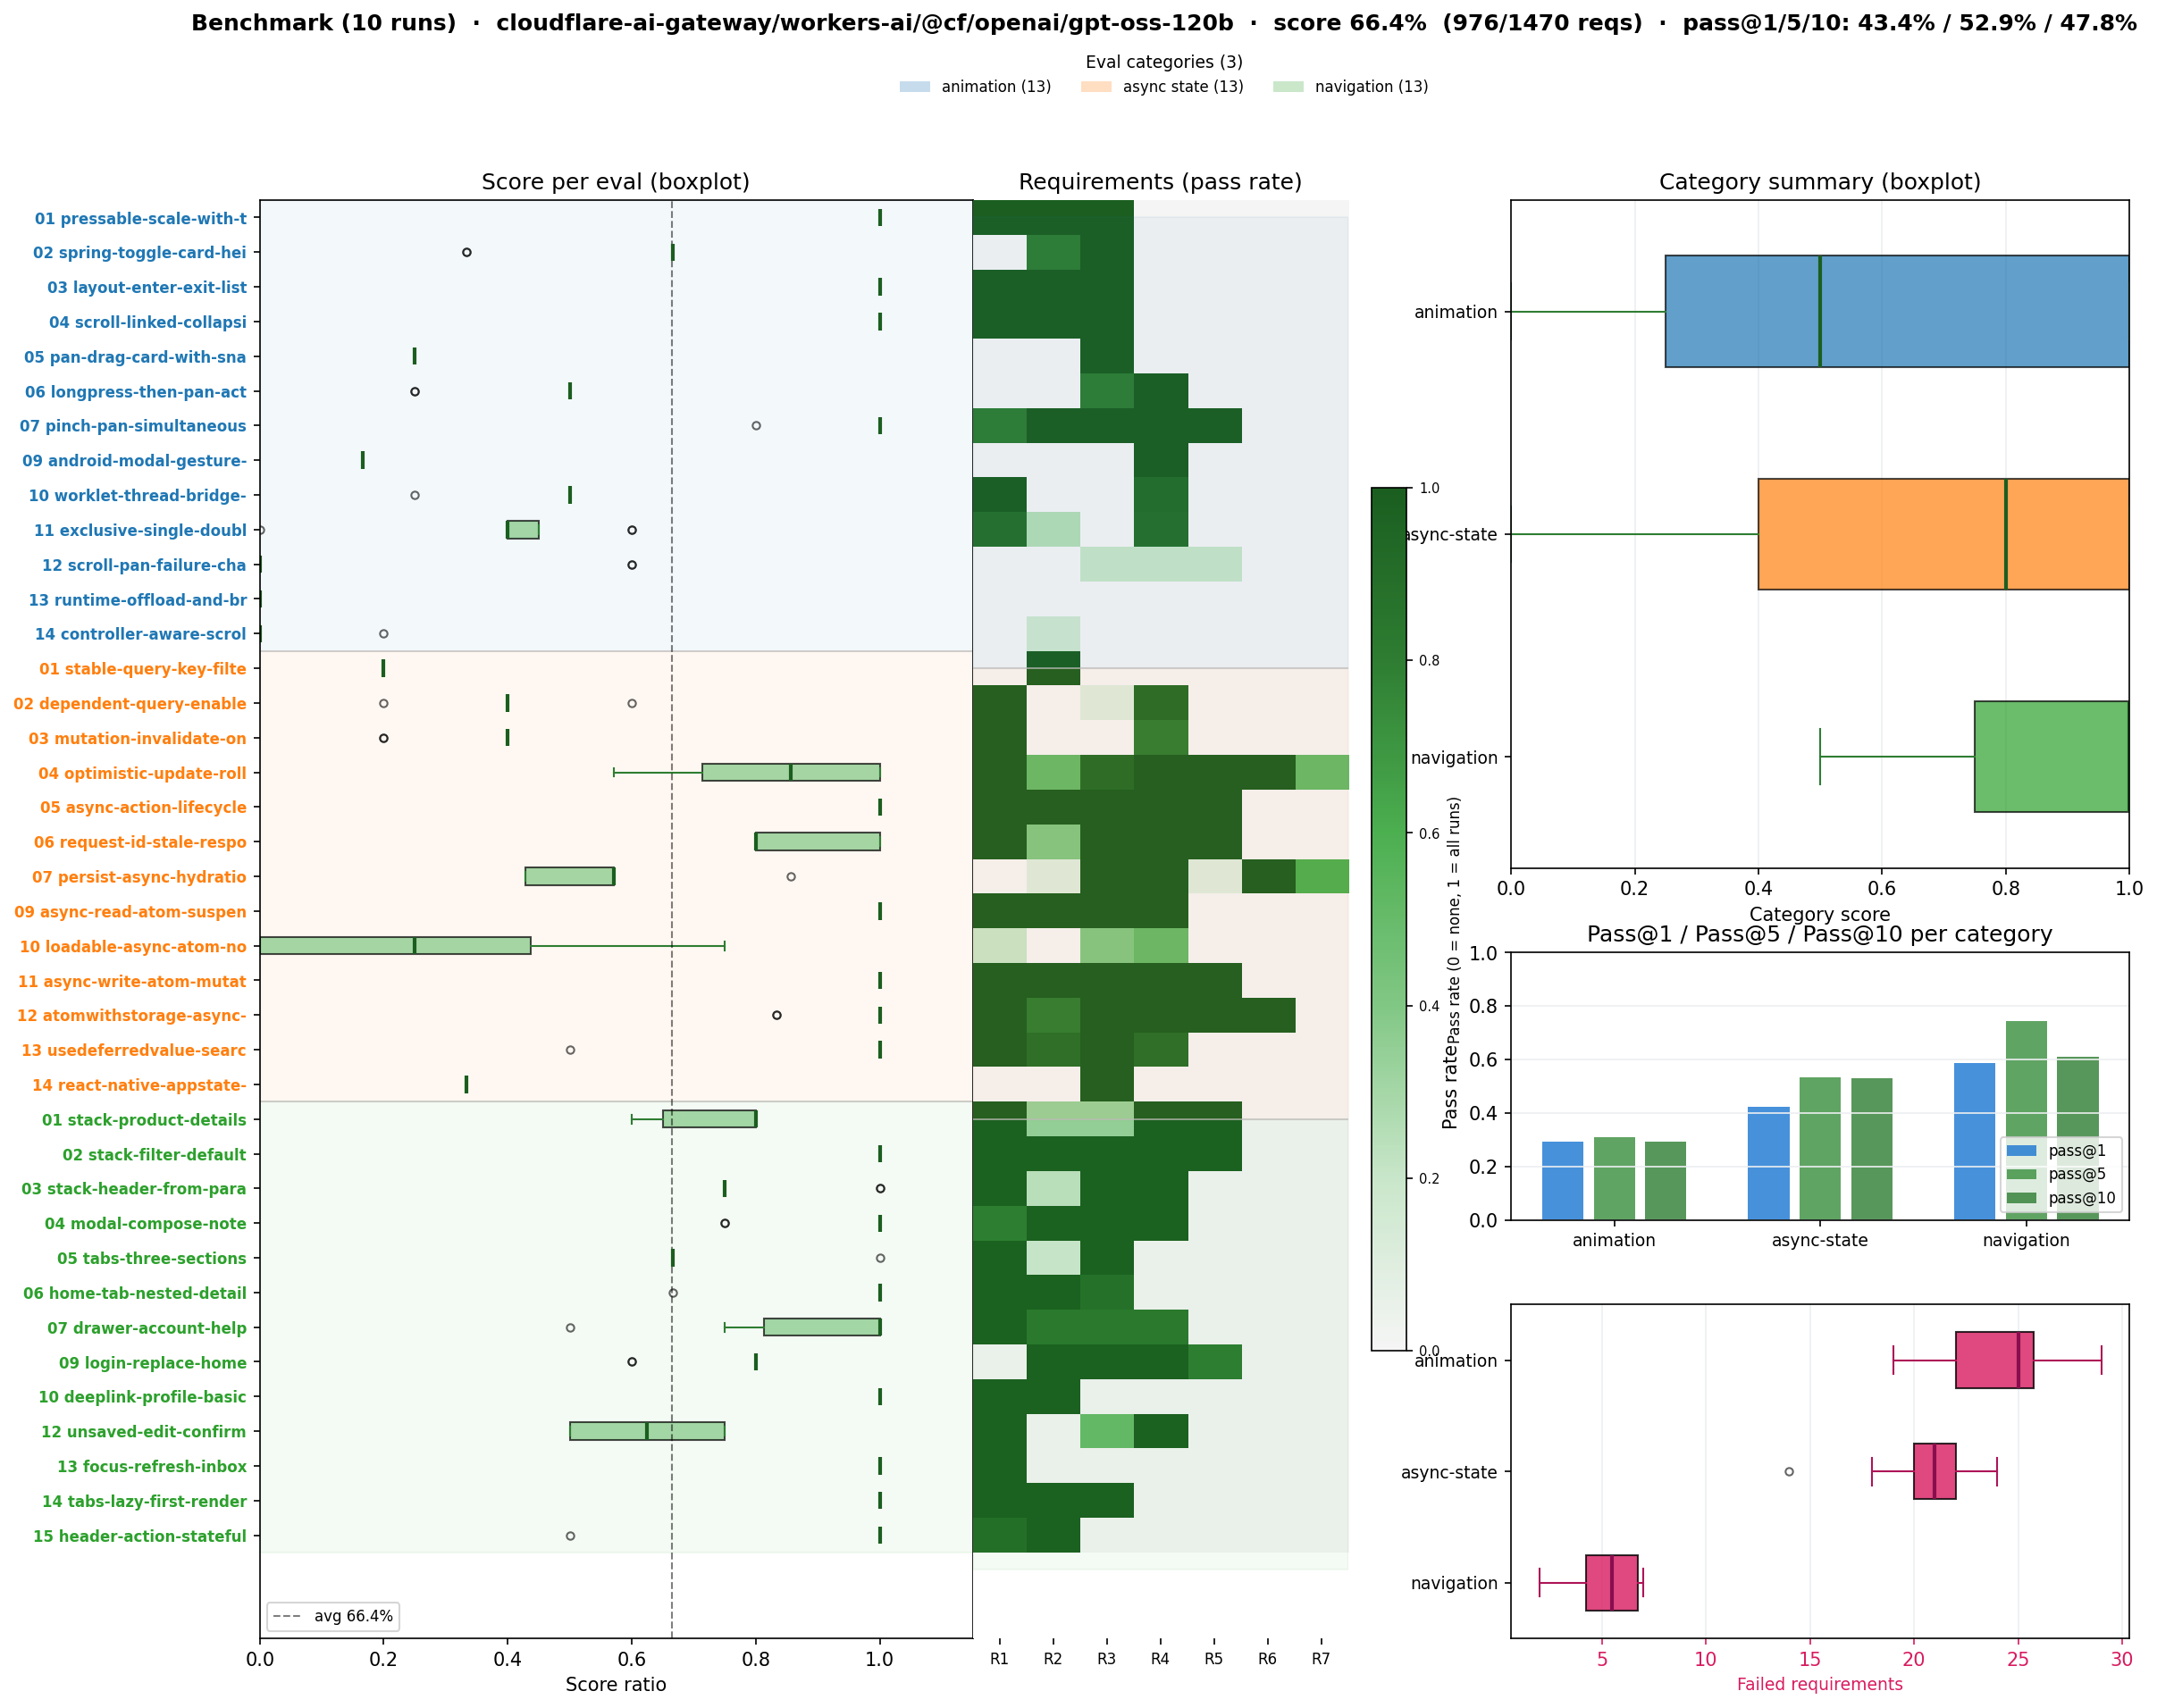
\includegraphics[width=\textwidth]{export/figures/gpt-oss-120b_benchmark_plot.png}
\caption{Benchmark Plot for gpt-oss-120b.}
\end{figure}

\begin{figure}[htbp]
\centering
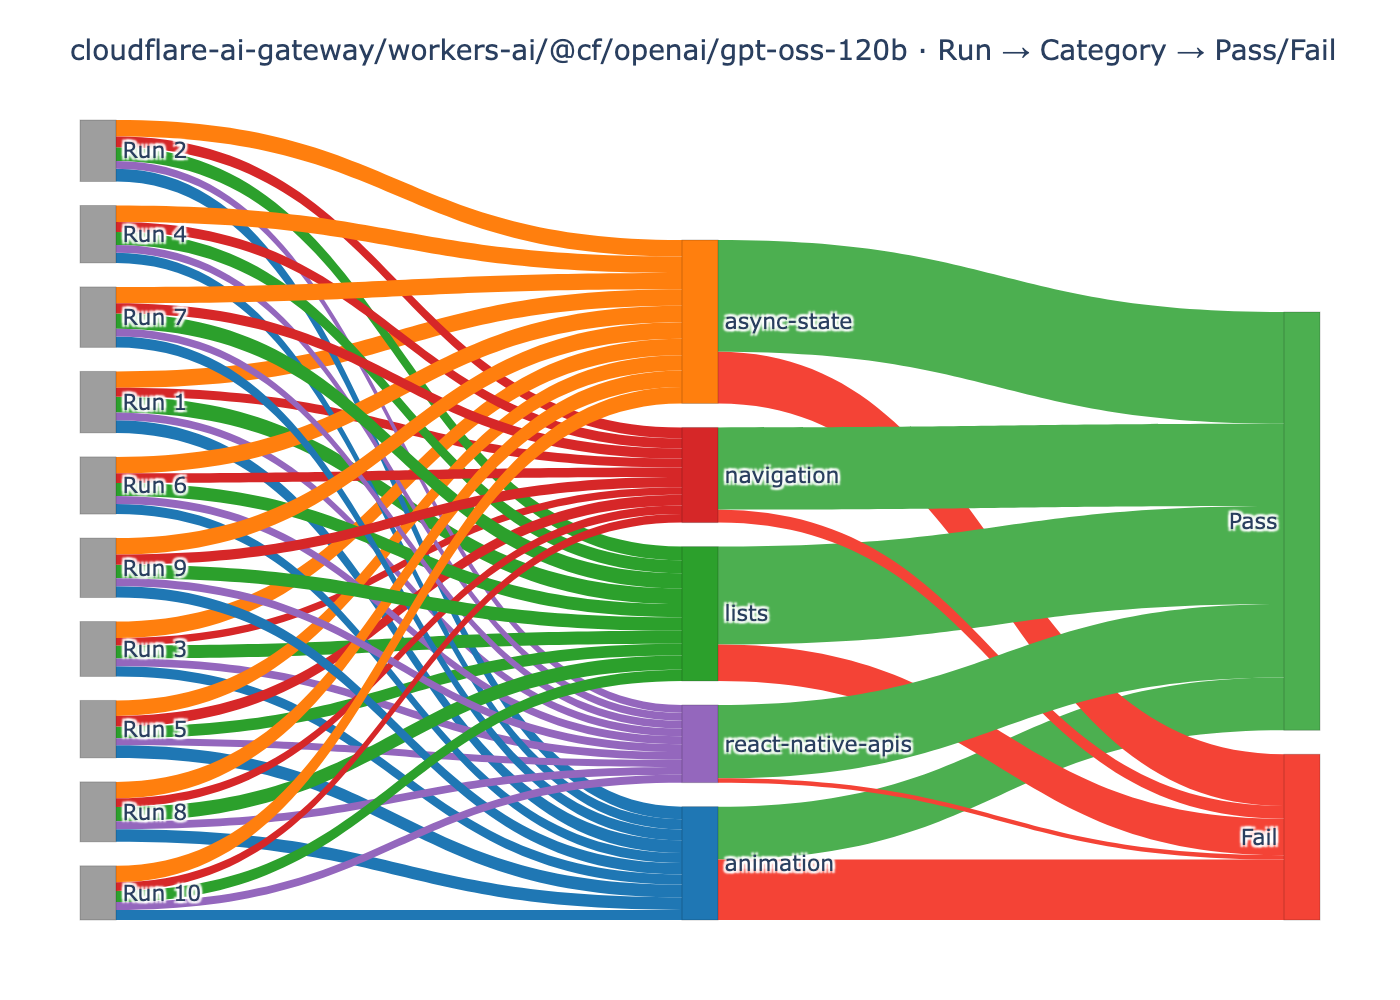
\includegraphics[width=\textwidth]{export/figures/gpt-oss-120b_sankey_per_run.png}
\caption{Sankey per run for gpt-oss-120b showing the distribution of evals with respect to categories and results}
\end{figure}


\clearpage

\subsection{gpt-oss-20b}

% Table: summary
% Requires: \usepackage{booktabs}
\begin{table}[htbp]
\centering
\begin{tabular}{lrrrrrr}
\toprule
Model & Runs & Score & Reqs & P@1 & P@5 & P@10 \\
\midrule
cloudflare-ai-gateway/workers-ai/@cf/openai/gpt-os & 10 & 71.0\% & 1761/2480 & 43.4\% & 56.2\% & 55.4\% \\
\bottomrule
\end{tabular}
\caption{Model summary for gpt-oss-20b}
\end{table}


% Table: category_summary
% Requires: \usepackage{booktabs}
\begin{table}[htbp]
\centering
\begin{tabular}{lrrrr}
\toprule
Category & Score & Evals & Requirements & Failed requirements \\
\midrule
animation & 51.7\% & 107 & 53 & 232 \\
async state & 65.8\% & 128 & 65 & 212 \\
navigation & 84.2\% & 94 & 45 & 61 \\
\bottomrule
\end{tabular}
\caption{Results by category for gpt-oss-20b. Score: mean(per-eval passed/total weight) across evals and runs. Evals: count of evaluation tasks. Requirements: sum of requirement count per eval. Failed requirements: sum of failed requirement instances across runs.}
\end{table}


% Table: per_eval
\input{export/tables/gpt-oss-20b_per_eval}

\begin{figure}[htbp]
\centering
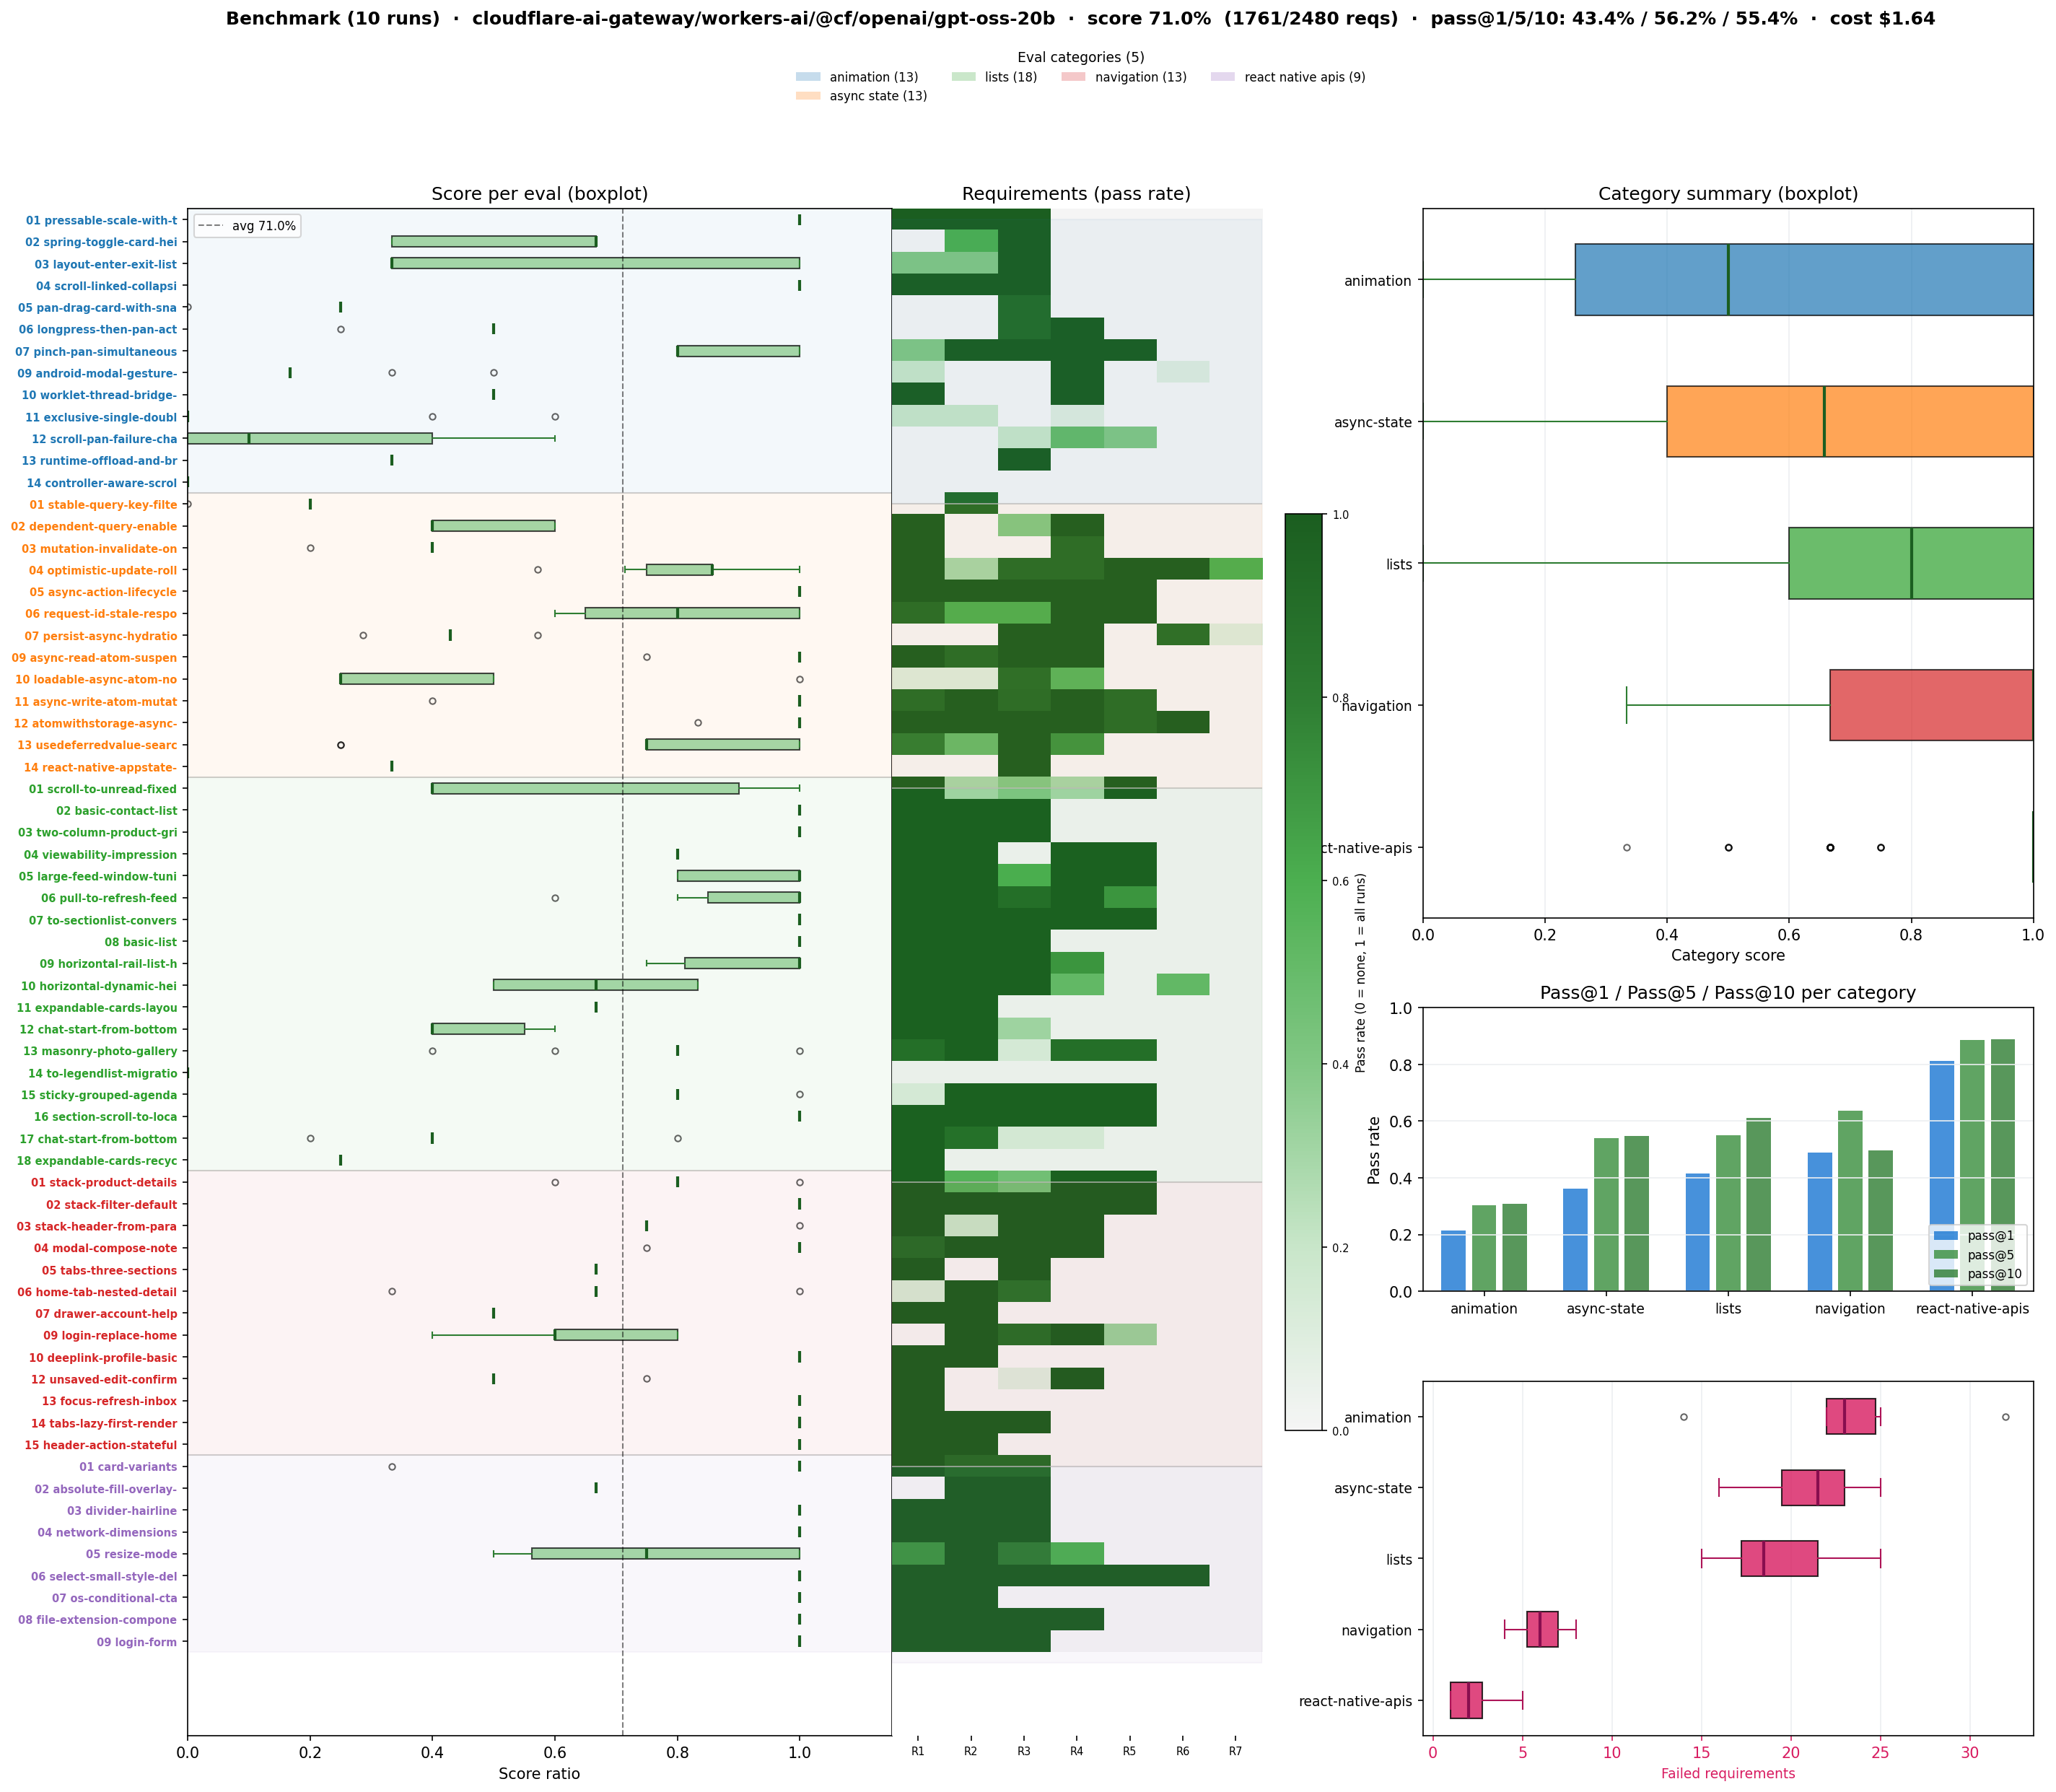
\includegraphics[width=\textwidth]{export/figures/gpt-oss-20b_benchmark_plot.png}
\caption{Benchmark Plot for gpt-oss-20b.}
\end{figure}

\begin{figure}[htbp]
\centering
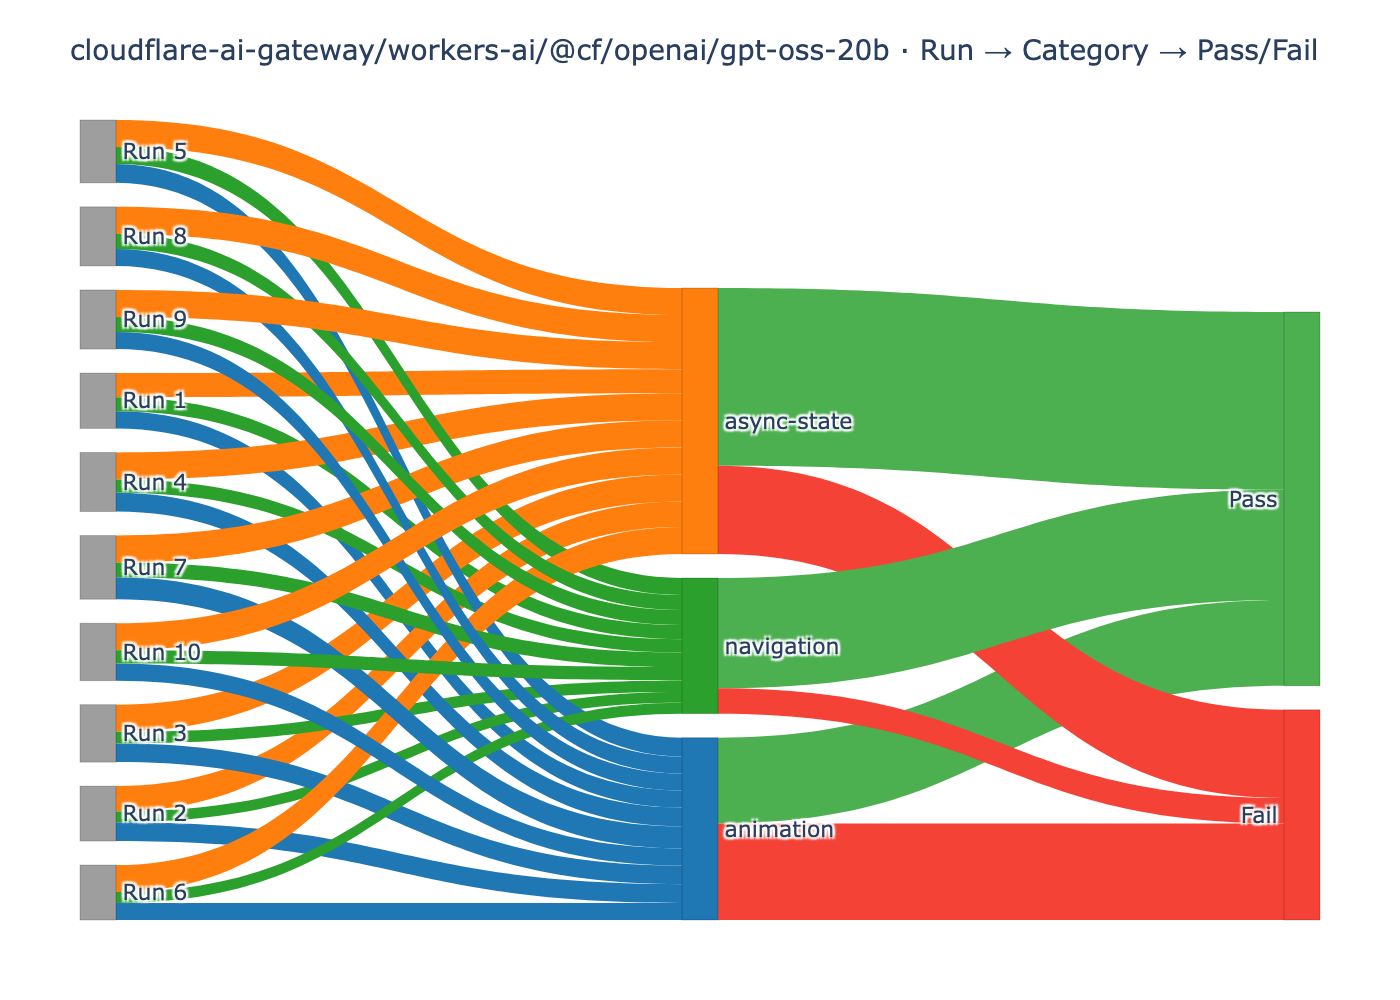
\includegraphics[width=\textwidth]{export/figures/gpt-oss-20b_sankey_per_run.png}
\caption{Sankey per run for gpt-oss-20b showing the distribution of evals with respect to categories and results}
\end{figure}


\clearpage

\subsection{grok-4}

% Table: summary
% Requires: \usepackage{booktabs}
\begin{table}[htbp]
\centering
\begin{tabular}{lrrrrrr}
\toprule
Model & Runs & Score & Reqs & P@1 & P@5 & P@10 \\
\midrule
vercel/xai/grok-4 & 10 & 70.1\% & 1142/1630 & 40.3\% & 50.3\% & 51.3\% \\
\bottomrule
\end{tabular}
\caption{Model summary for grok-4}
\end{table}


% Table: category_summary
% Requires: \usepackage{booktabs}
\begin{table}[htbp]
\centering
\begin{tabular}{lrrrr}
\toprule
Category & Score & Evals & Requirements & Failed requirements \\
\midrule
animation & 60.7\% & 130 & 53 & 226 \\
async state & 70.1\% & 130 & 65 & 187 \\
lists & 69.6\% & 180 & 79 & 237 \\
navigation & 84.9\% & 130 & 45 & 75 \\
react native apis & 92.1\% & 89 & 31 & 21 \\
\bottomrule
\end{tabular}
\caption{Results by category for grok-4. Score: mean(per-eval passed/total weight) across evals and runs. Evals: count of evaluation tasks. Requirements: sum of requirement count per eval. Failed requirements: sum of failed requirement instances across runs.}
\end{table}


% Table: per_eval
\input{export/tables/grok-4_per_eval}

\begin{figure}[htbp]
\centering
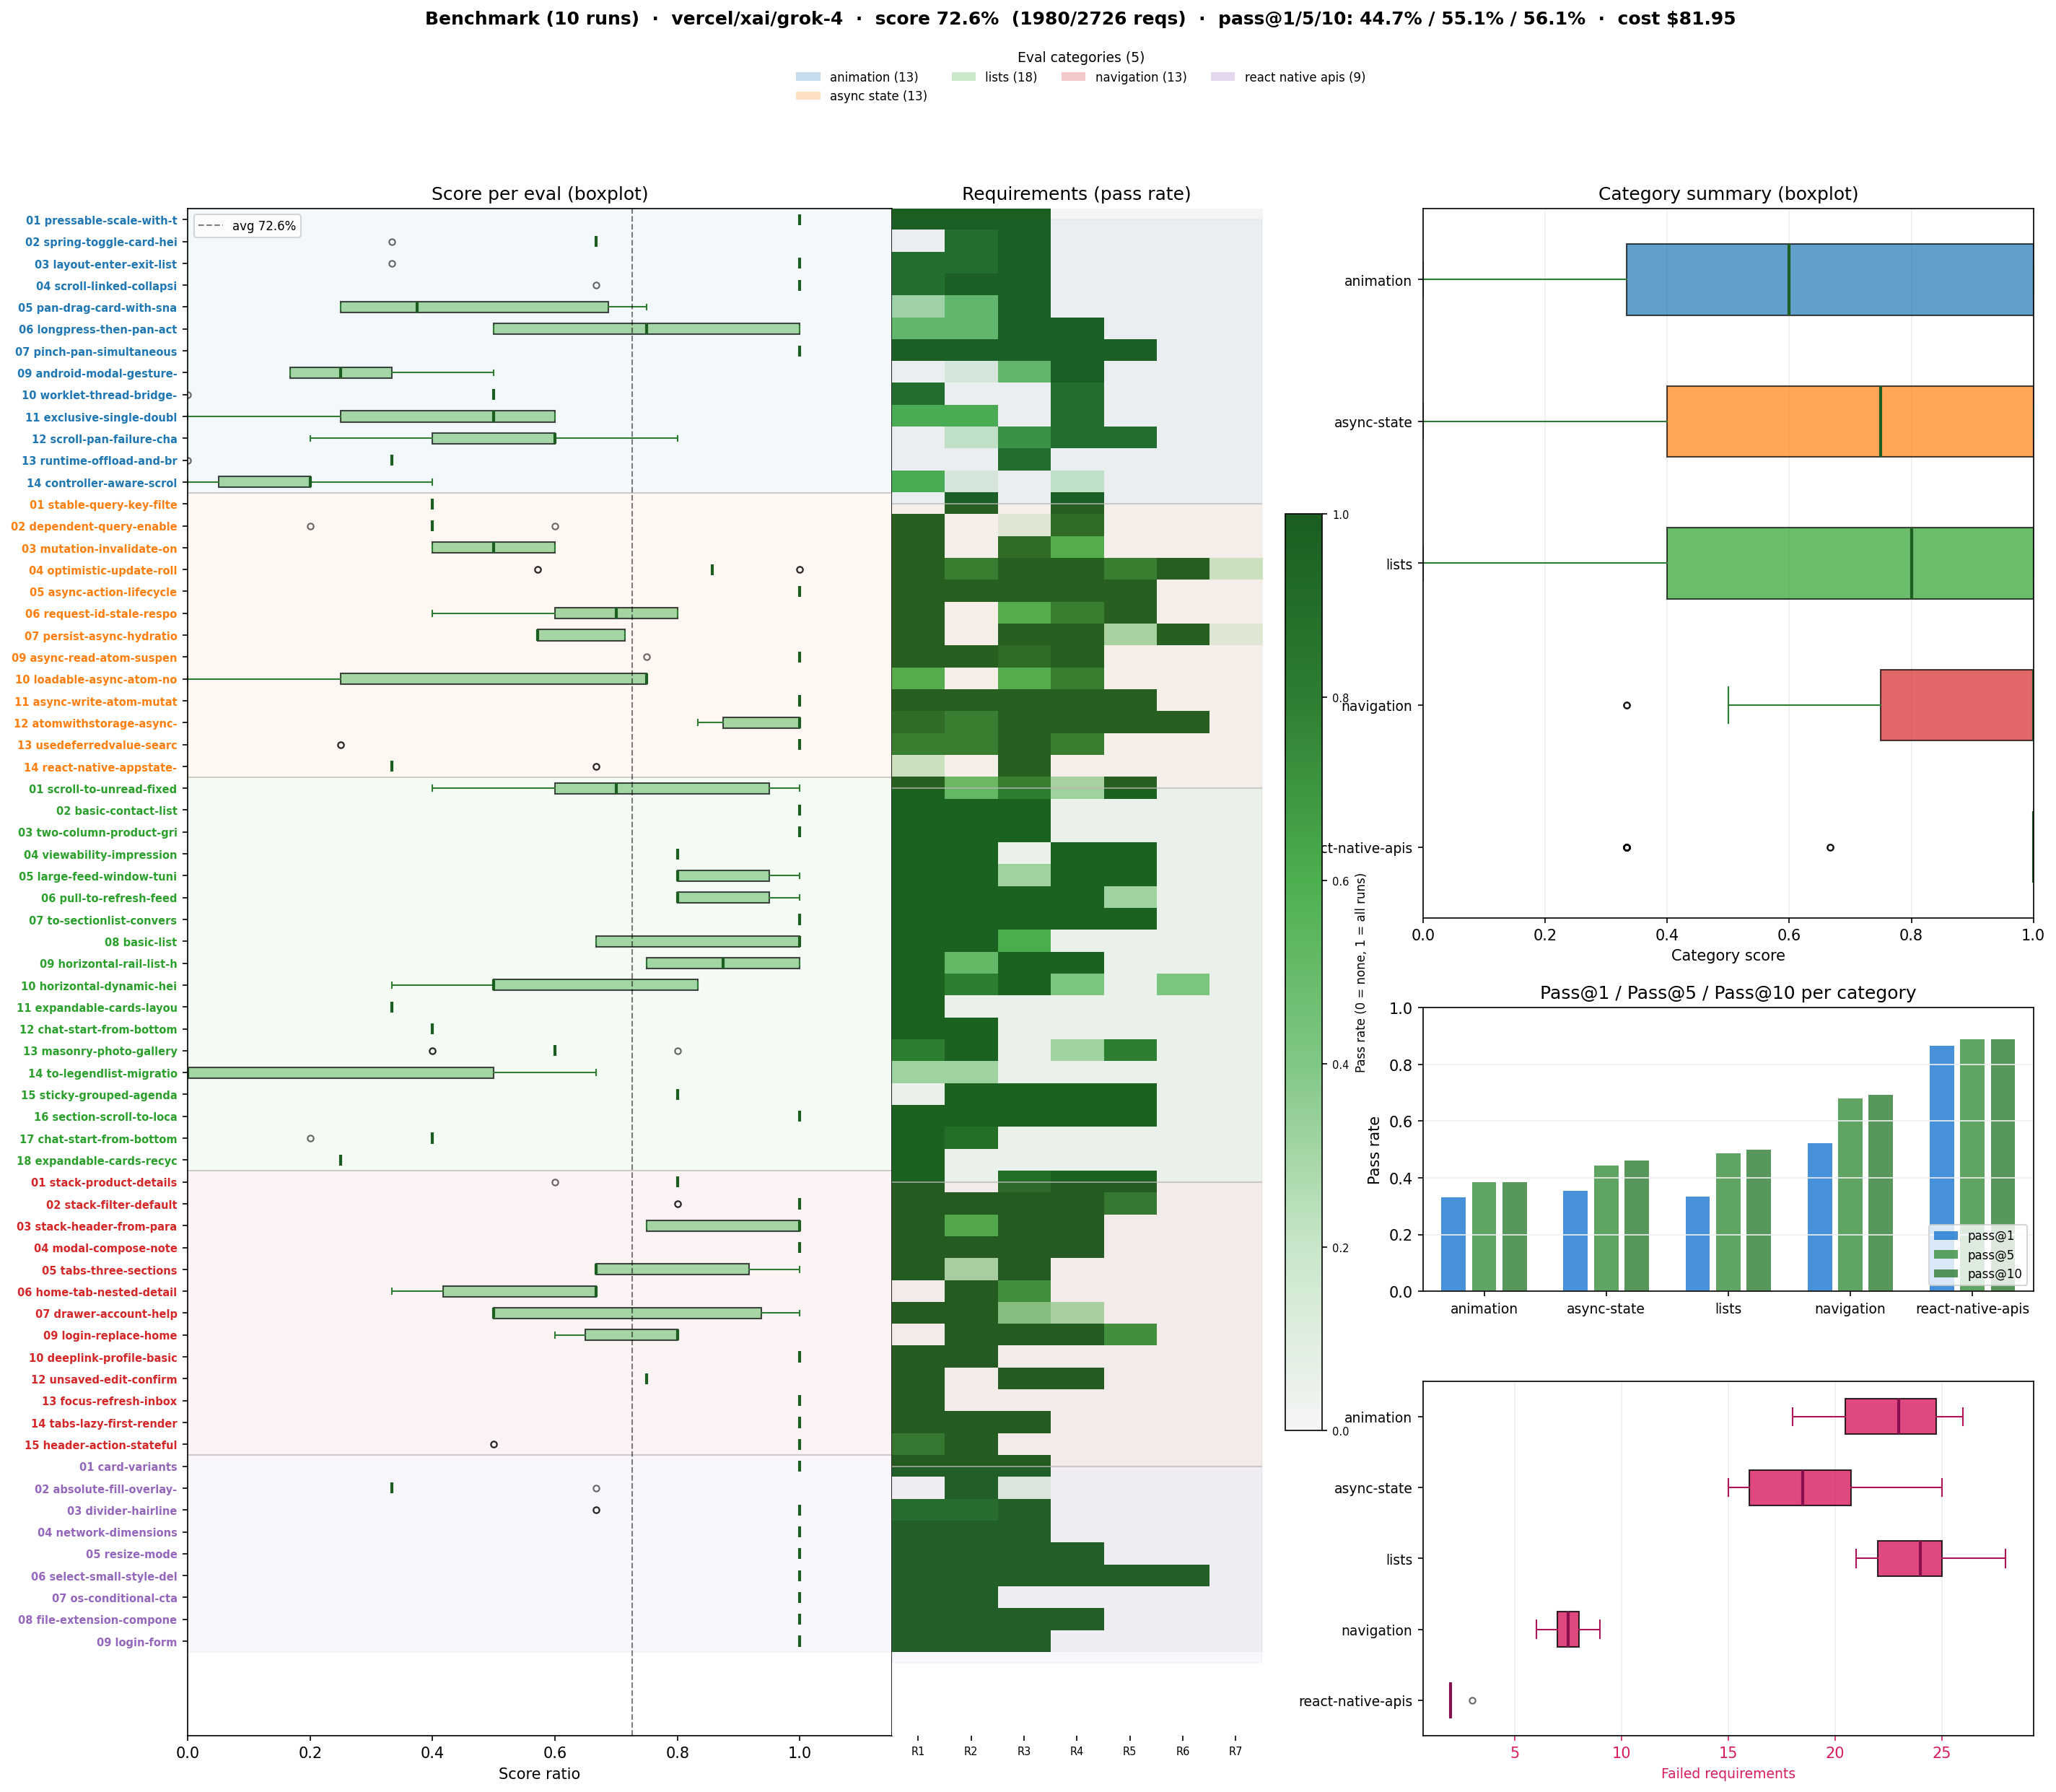
\includegraphics[width=\textwidth]{export/figures/grok-4_benchmark_plot.png}
\caption{Benchmark Plot for grok-4.}
\end{figure}

\begin{figure}[htbp]
\centering
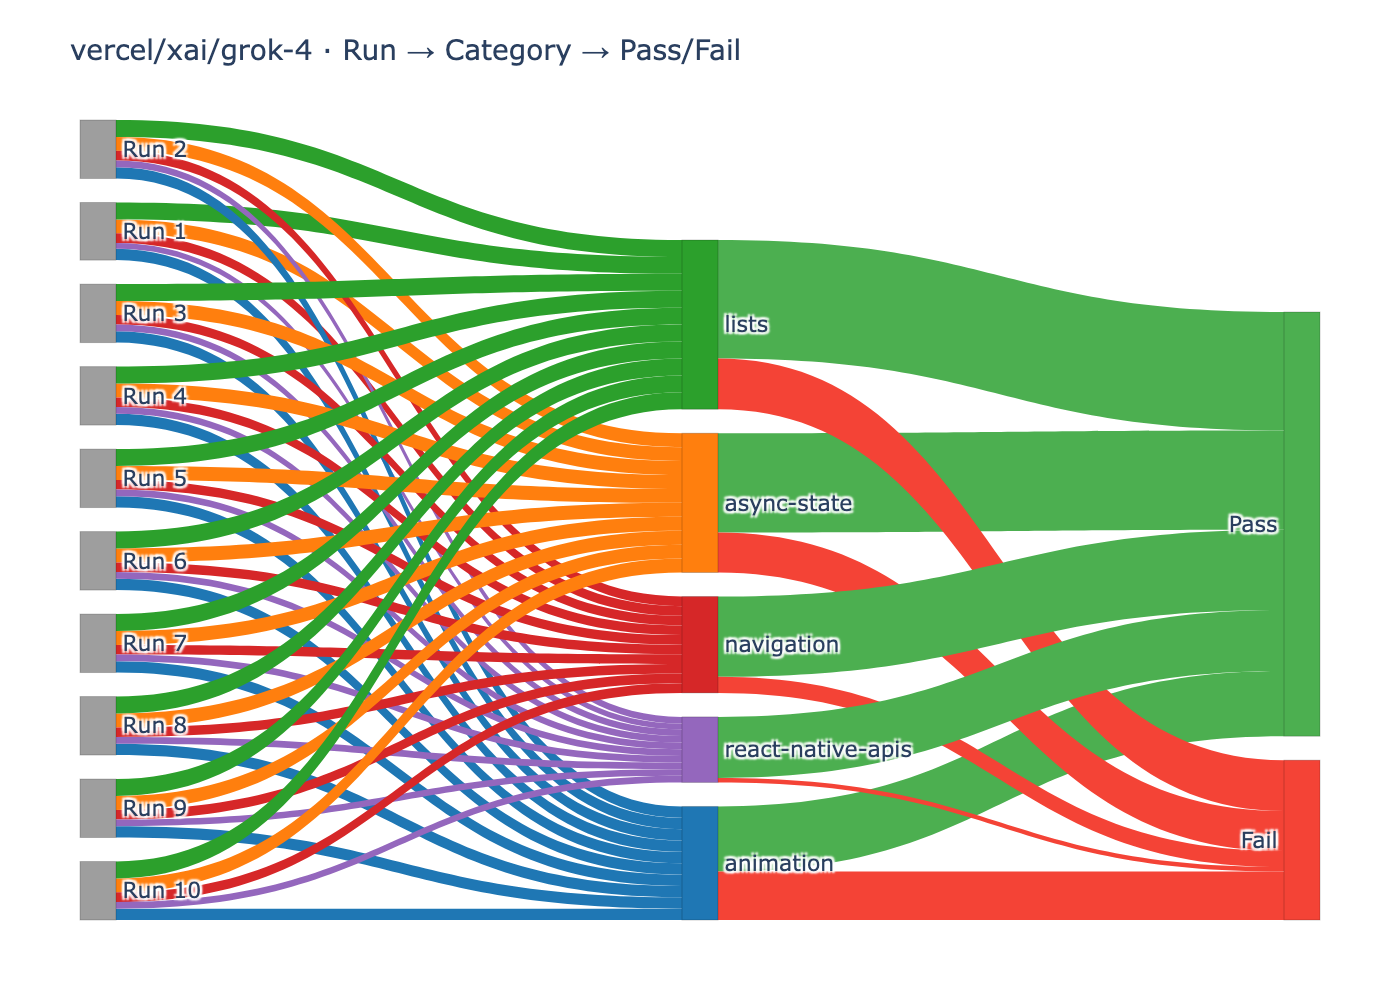
\includegraphics[width=\textwidth]{export/figures/grok-4_sankey_per_run.png}
\caption{Sankey per run for grok-4 showing the distribution of evals with respect to categories and results}
\end{figure}


\clearpage

\subsection{kimi-k2.5}

% Table: summary
% Requires: \usepackage{booktabs}
\begin{table}[htbp]
\centering
\begin{tabular}{lrrrrrr}
\toprule
Model & Runs & Score & Reqs & P@1 & P@5 & P@10 \\
\midrule
vercel/moonshotai/kimi-k2.5 & 10 & 74.9\% & 1221/1630 & 50.5\% & 66.2\% & 69.2\% \\
\bottomrule
\end{tabular}
\caption{Model summary for kimi-k2.5}
\end{table}


% Table: category_summary
% Requires: \usepackage{booktabs}
\begin{table}[htbp]
\centering
\begin{tabular}{lrrrr}
\toprule
Category & Score & Evals & Requirements & Failed requirements \\
\midrule
animation & 61.0\% & 130 & 53 & 220 \\
async state & 76.0\% & 130 & 65 & 148 \\
lists & 77.7\% & 180 & 79 & 181 \\
navigation & 91.9\% & 130 & 45 & 41 \\
react native apis & 88.3\% & 90 & 31 & 33 \\
\bottomrule
\end{tabular}
\caption{Results by category for kimi-k2.5. Score: mean(per-eval passed/total weight) across evals and runs. Evals: count of evaluation tasks. Requirements: sum of requirement count per eval. Failed requirements: sum of failed requirement instances across runs.}
\end{table}


% Table: per_eval
% Requires: \usepackage{booktabs}
\begin{table}[htbp]
\centering
\begin{adjustbox}{width=0.8\textwidth}
\begin{tabular}{lrrrrr}
\toprule
Eval & Category & Score & P@1 & P@5 & P@10 \\
\midrule
01-rn-anim-pressable-scale-with-timing & animation & 100.0\% & 100.0\% & 100.0\% & 100.0\% \\
02-rn-anim-spring-toggle-card-height & animation & 66.7\% & 30.0\% & 91.7\% & 100.0\% \\
03-rn-anim-layout-enter-exit-list-items & animation & 100.0\% & 100.0\% & 100.0\% & 100.0\% \\
04-rn-anim-scroll-linked-collapsing-header & animation & 73.3\% & 40.0\% & 97.6\% & 100.0\% \\
05-rn-anim-pan-drag-card-with-snap-points & animation & 55.0\% & 0.0\% & 0.0\% & 0.0\% \\
06-rn-anim-longpress-then-pan-activation-gate & animation & 72.5\% & 40.0\% & 97.6\% & 100.0\% \\
07-rn-anim-pinch-pan-simultaneous-photo-canvas & animation & 100.0\% & 100.0\% & 100.0\% & 100.0\% \\
09-rn-anim-android-modal-gesture-root-safety & animation & 30.0\% & 0.0\% & 0.0\% & 0.0\% \\
10-rn-anim-worklet-thread-bridge-schedule-on-rn & animation & 20.0\% & 0.0\% & 0.0\% & 0.0\% \\
11-rn-rngh-exclusive-single-double-tap & animation & 38.0\% & 0.0\% & 0.0\% & 0.0\% \\
12-rn-rngh-scroll-pan-failure-chain & animation & 70.0\% & 0.0\% & 0.0\% & 0.0\% \\
13-rn-worklets-runtime-offload-and-bridge & animation & 33.3\% & 0.0\% & 0.0\% & 0.0\% \\
14-rn-keyboard-controller-aware-scroll-footer & animation & 34.0\% & 0.0\% & 0.0\% & 0.0\% \\
01-rn-rq-stable-query-key-filters & async state & 40.0\% & 0.0\% & 0.0\% & 0.0\% \\
02-rn-rq-dependent-query-enabled-gate & async state & 46.0\% & 0.0\% & 0.0\% & 0.0\% \\
03-rn-rq-mutation-invalidate-on-success & async state & 68.0\% & 0.0\% & 0.0\% & 0.0\% \\
04-rn-rq-optimistic-update-rollback & async state & 98.6\% & 90.0\% & 100.0\% & 100.0\% \\
05-rn-zustand-async-action-lifecycle & async state & 100.0\% & 100.0\% & 100.0\% & 100.0\% \\
06-rn-zustand-request-id-stale-response-guard & async state & 68.0\% & 20.0\% & 77.8\% & 100.0\% \\
07-rn-zustand-persist-async-hydration-gate & async state & 72.9\% & 30.0\% & 91.7\% & 100.0\% \\
09-rn-jotai-async-read-atom-suspense & async state & 97.5\% & 90.0\% & 100.0\% & 100.0\% \\
10-rn-jotai-loadable-async-atom-no-suspense & async state & 50.0\% & 0.0\% & 0.0\% & 0.0\% \\
11-rn-jotai-async-write-atom-mutation & async state & 100.0\% & 100.0\% & 100.0\% & 100.0\% \\
12-rn-jotai-atomwithstorage-async-rehydrate-guard & async state & 93.3\% & 60.0\% & 100.0\% & 100.0\% \\
13-rn-react-usedeferredvalue-search-stale-indicator & async state & 100.0\% & 100.0\% & 100.0\% & 100.0\% \\
14-rn-rq-react-native-appstate-focus-online-managers & async state & 53.3\% & 0.0\% & 0.0\% & 0.0\% \\
01-rn-flatlist-scroll-to-unread-fixed-rows & lists & 90.0\% & 70.0\% & 100.0\% & 100.0\% \\
02-rn-flatlist-basic-contact-list & lists & 100.0\% & 100.0\% & 100.0\% & 100.0\% \\
03-rn-flatlist-two-column-product-grid & lists & 100.0\% & 100.0\% & 100.0\% & 100.0\% \\
04-rn-flatlist-viewability-impression-tracking & lists & 80.0\% & 0.0\% & 0.0\% & 0.0\% \\
05-rn-flatlist-large-feed-window-tuning & lists & 86.0\% & 30.0\% & 91.7\% & 100.0\% \\
06-rn-flatlist-pull-to-refresh-feed & lists & 84.0\% & 20.0\% & 77.8\% & 100.0\% \\
07-rn-flatlist-to-sectionlist-conversion & lists & 86.0\% & 30.0\% & 91.7\% & 100.0\% \\
08-rn-flashlist-basic-list & lists & 100.0\% & 100.0\% & 100.0\% & 100.0\% \\
09-rn-flashlist-horizontal-rail-list-header & lists & 80.0\% & 20.0\% & 77.8\% & 100.0\% \\
10-rn-flashlist-horizontal-dynamic-height-header-first-item & lists & 83.3\% & 0.0\% & 0.0\% & 0.0\% \\
11-rn-flashlist-expandable-cards-layout-state & lists & 60.0\% & 0.0\% & 0.0\% & 0.0\% \\
12-rn-flashlist-chat-start-from-bottom & lists & 54.0\% & 0.0\% & 0.0\% & 0.0\% \\
13-rn-flashlist-masonry-photo-gallery & lists & 60.0\% & 0.0\% & 0.0\% & 0.0\% \\
14-rn-flatlist-to-legendlist-migration & lists & 70.0\% & 10.0\% & 50.0\% & 100.0\% \\
15-rn-legendlist-sticky-grouped-agenda & lists & 82.0\% & 20.0\% & 77.8\% & 100.0\% \\
16-rn-legendlist-section-scroll-to-location & lists & 100.0\% & 100.0\% & 100.0\% & 100.0\% \\
17-rn-legendlist-chat-start-from-bottom & lists & 40.0\% & 0.0\% & 0.0\% & 0.0\% \\
18-rn-legendlist-expandable-cards-recycling-state & lists & 42.5\% & 0.0\% & 0.0\% & 0.0\% \\
01-rn-nav-stack-product-details & navigation & 78.0\% & 20.0\% & 77.8\% & 100.0\% \\
02-rn-nav-stack-filter-default & navigation & 100.0\% & 100.0\% & 100.0\% & 100.0\% \\
03-rn-nav-stack-header-from-param & navigation & 87.5\% & 50.0\% & 99.6\% & 100.0\% \\
04-rn-nav-modal-compose-note & navigation & 100.0\% & 100.0\% & 100.0\% & 100.0\% \\
05-rn-nav-tabs-three-sections & navigation & 100.0\% & 100.0\% & 100.0\% & 100.0\% \\
06-rn-nav-home-tab-nested-details & navigation & 86.7\% & 60.0\% & 100.0\% & 100.0\% \\
07-rn-nav-drawer-account-help & navigation & 100.0\% & 100.0\% & 100.0\% & 100.0\% \\
09-rn-nav-login-replace-home & navigation & 72.0\% & 10.0\% & 50.0\% & 100.0\% \\
10-rn-nav-deeplink-profile-basic & navigation & 95.0\% & 90.0\% & 100.0\% & 100.0\% \\
12-rn-nav-unsaved-edit-confirm & navigation & 95.0\% & 80.0\% & 100.0\% & 100.0\% \\
13-rn-nav-focus-refresh-inbox & navigation & 100.0\% & 100.0\% & 100.0\% & 100.0\% \\
14-rn-nav-tabs-lazy-first-render & navigation & 100.0\% & 100.0\% & 100.0\% & 100.0\% \\
15-rn-nav-header-action-stateful & navigation & 80.0\% & 60.0\% & 100.0\% & 100.0\% \\
01-rn-stylesheet-card-variants & react native apis & 100.0\% & 100.0\% & 100.0\% & 100.0\% \\
02-rn-stylesheet-absolute-fill-overlay-badge & react native apis & 40.0\% & 0.0\% & 0.0\% & 0.0\% \\
03-rn-stylesheet-divider-hairline & react native apis & 70.0\% & 20.0\% & 77.8\% & 100.0\% \\
04-rn-image-network-dimensions & react native apis & 100.0\% & 100.0\% & 100.0\% & 100.0\% \\
05-rn-imagebackground-resize-mode & react native apis & 85.0\% & 70.0\% & 100.0\% & 100.0\% \\
06-rn-platform-select-small-style-delta & react native apis & 100.0\% & 100.0\% & 100.0\% & 100.0\% \\
07-rn-platform-os-conditional-cta & react native apis & 100.0\% & 100.0\% & 100.0\% & 100.0\% \\
08-rn-platform-file-extension-component-split & react native apis & 100.0\% & 100.0\% & 100.0\% & 100.0\% \\
09-rn-keyboardavoidingview-login-form & react native apis & 100.0\% & 100.0\% & 100.0\% & 100.0\% \\
\bottomrule
\end{tabular}
\end{adjustbox}
\caption{Per-eval results (score and pass@k) for kimi-k2.5}
\end{table}


\begin{figure}[htbp]
\centering
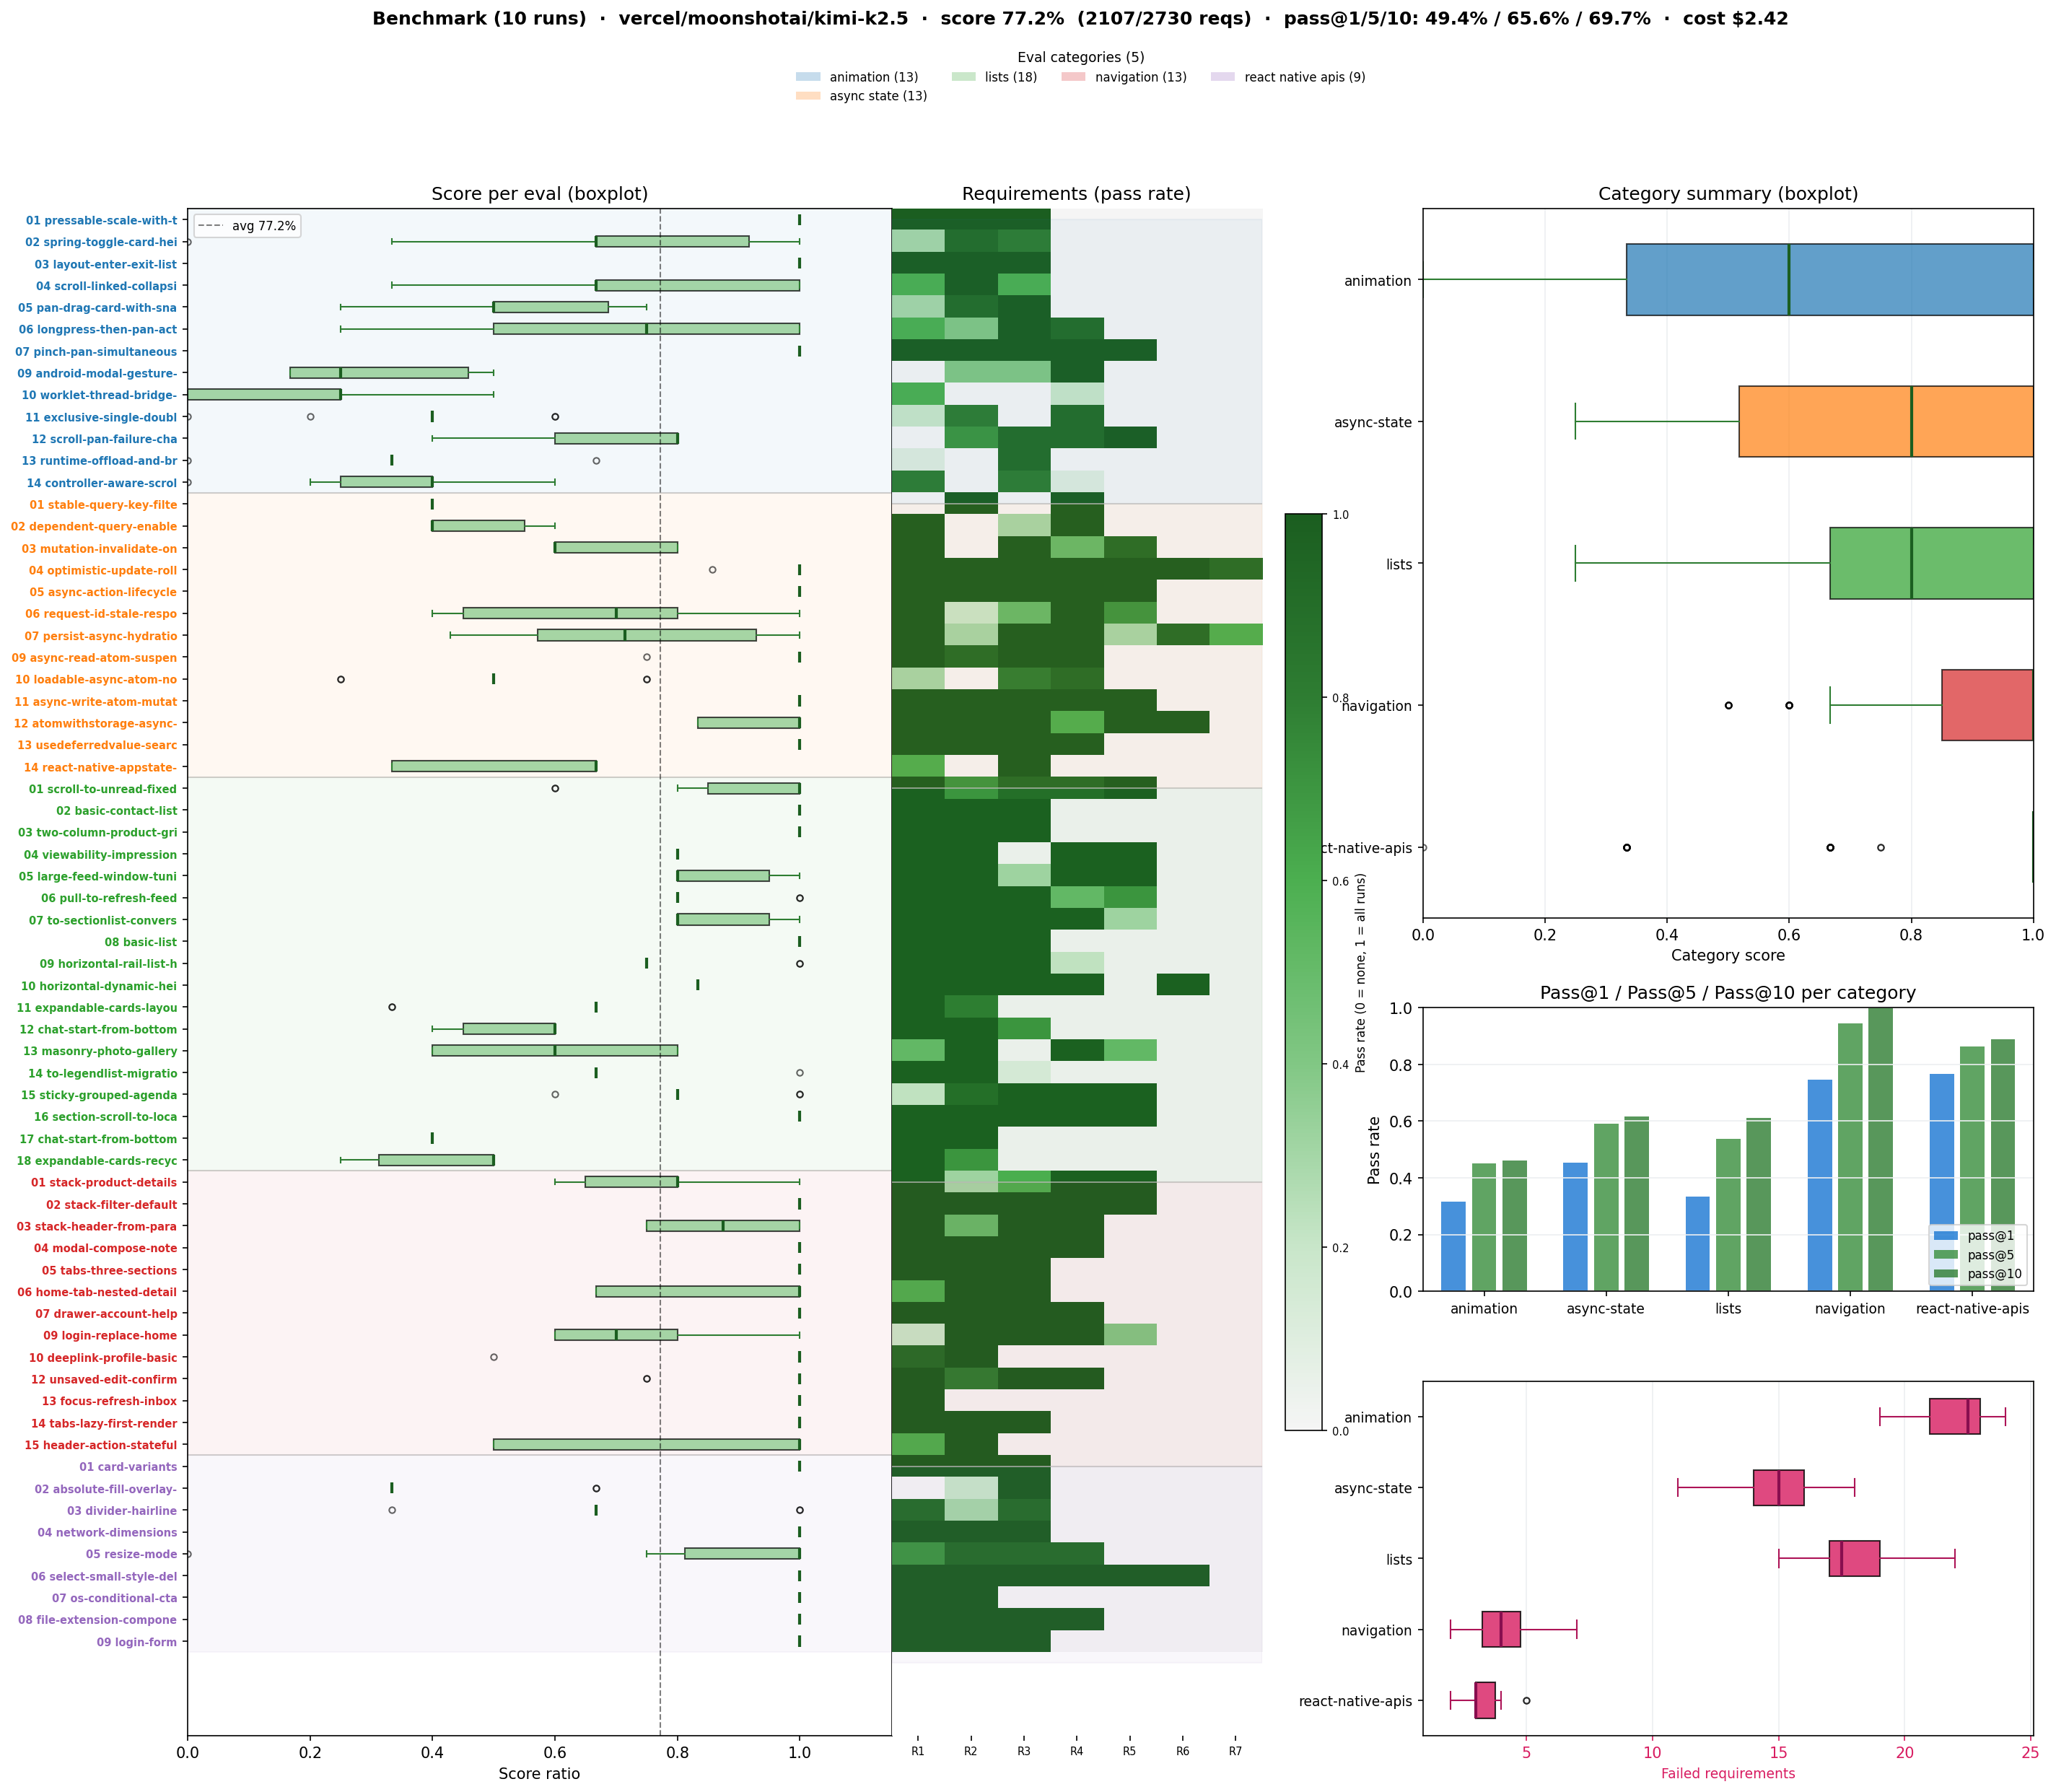
\includegraphics[width=\textwidth]{export/figures/kimi-k2.5_benchmark_plot.png}
\caption{Benchmark Plot for kimi-k2.5.}
\end{figure}

\begin{figure}[htbp]
\centering
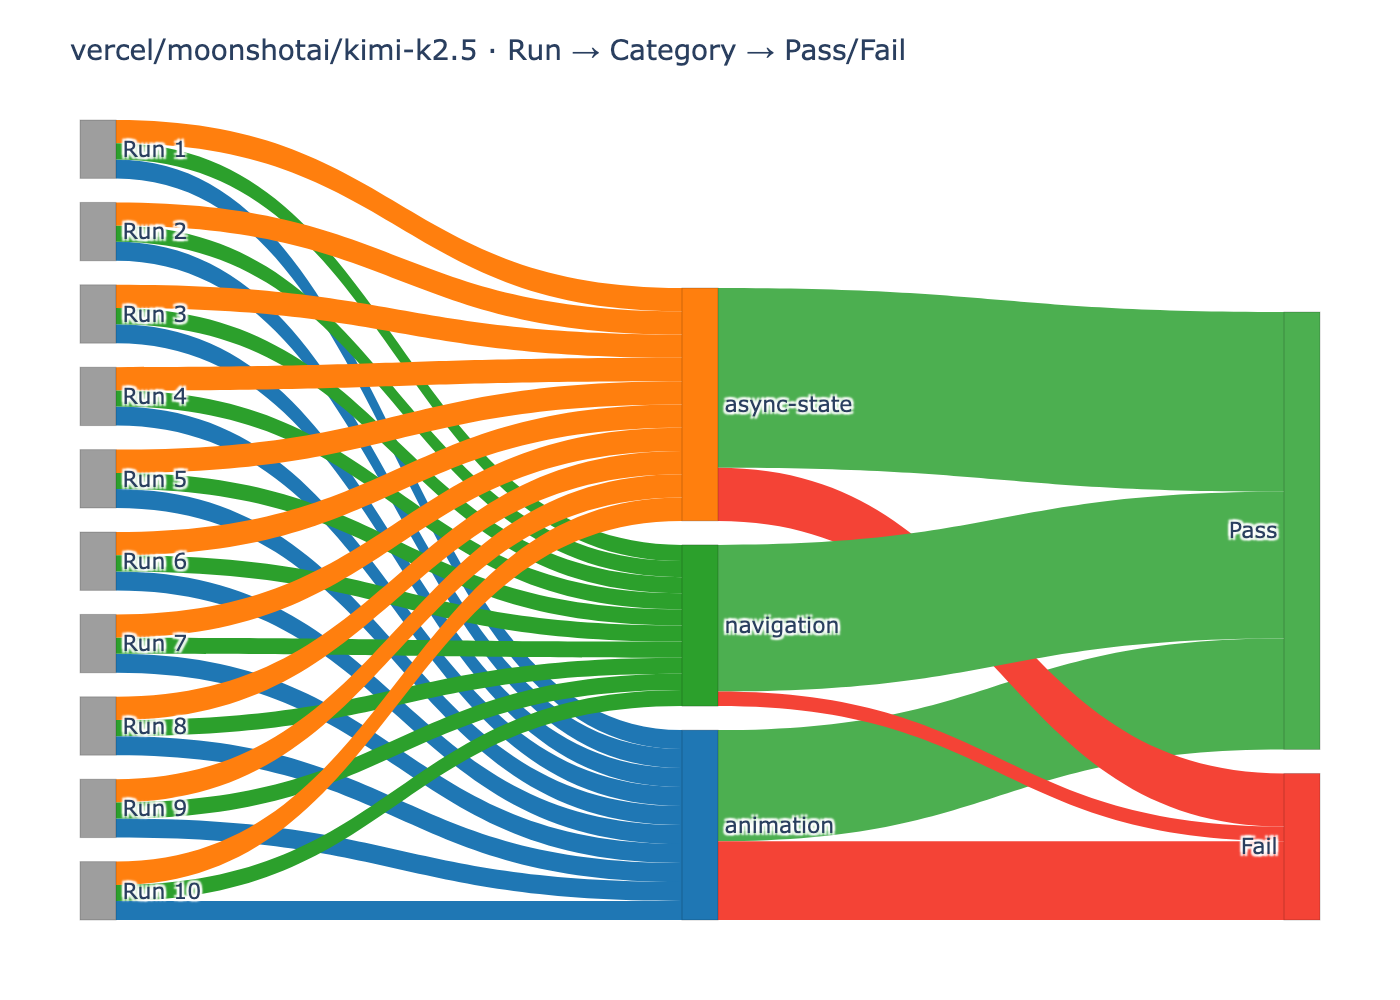
\includegraphics[width=\textwidth]{export/figures/kimi-k2.5_sankey_per_run.png}
\caption{Sankey per run for kimi-k2.5 showing the distribution of evals with respect to categories and results}
\end{figure}


\clearpage

\subsection{qwen2.5-coder-32b-instruct}

% Table: summary
% Requires: \usepackage{booktabs}
\begin{table}[htbp]
\centering
\begin{tabular}{lrrrrrr}
\toprule
Model & Runs & Score & Reqs & P@1 & P@5 & P@10 \\
\midrule
cloudflare-ai-gateway/workers-ai/@cf/qwen/qwen2.5- & 10 & 51.2\% & 1316/2570 & 18.8\% & 29.3\% & 28.8\% \\
\bottomrule
\end{tabular}
\caption{Model summary for qwen2.5-coder-32b-instruct}
\end{table}


% Table: category_summary
% Requires: \usepackage{booktabs}
\begin{table}[htbp]
\centering
\begin{tabular}{lrrrr}
\toprule
Category & Score & Evals & Requirements & Failed requirements \\
\midrule
animation & 25.9\% & 122 & 53 & 389 \\
async state & 44.4\% & 121 & 65 & 329 \\
lists & 57.3\% & 176 & 79 & 318 \\
navigation & 66.1\% & 111 & 45 & 140 \\
react native apis & 70.2\% & 86 & 31 & 78 \\
\bottomrule
\end{tabular}
\caption{Results by category for qwen2.5-coder-32b-instruct. Score: mean(per-eval passed/total weight) across evals and runs. Evals: count of evaluation tasks. Requirements: sum of requirement count per eval. Failed requirements: sum of failed requirement instances across runs.}
\end{table}


% Table: per_eval
% Requires: \usepackage{booktabs}
\begin{table}[htbp]
\centering
\begin{tabular}{lrrrrr}
\toprule
Eval & Category & Score & P@1 & P@5 & P@10 \\
\midrule
01-rn-anim-pressable-scale-with-timing & animation & 53.3\% & 0.0\% & 0.0\% & 0.0\% \\
02-rn-anim-spring-toggle-card-height & animation & 40.7\% & 0.0\% & 0.0\% & 0.0\% \\
03-rn-anim-layout-enter-exit-list-items & animation & 90.0\% & 80.0\% & 100.0\% & 100.0\% \\
04-rn-anim-scroll-linked-collapsing-header & animation & 46.7\% & 20.0\% & 77.8\% & 100.0\% \\
05-rn-anim-pan-drag-card-with-snap-points & animation & 10.0\% & 0.0\% & 0.0\% & 0.0\% \\
06-rn-anim-longpress-then-pan-activation-gate & animation & 22.5\% & 0.0\% & 0.0\% & 0.0\% \\
07-rn-anim-pinch-pan-simultaneous-photo-canvas & animation & 48.0\% & 0.0\% & 0.0\% & 0.0\% \\
09-rn-anim-android-modal-gesture-root-safety & animation & 3.7\% & 0.0\% & 0.0\% & 0.0\% \\
10-rn-anim-worklet-thread-bridge-schedule-on-rn & animation & 17.5\% & 0.0\% & 0.0\% & 0.0\% \\
11-rn-rngh-exclusive-single-double-tap & animation & 2.0\% & 0.0\% & 0.0\% & 0.0\% \\
12-rn-rngh-scroll-pan-failure-chain & animation & 4.4\% & 0.0\% & 0.0\% & 0.0\% \\
13-rn-worklets-runtime-offload-and-bridge & animation & 6.7\% & 0.0\% & 0.0\% & 0.0\% \\
14-rn-keyboard-controller-aware-scroll-footer & animation & 2.0\% & 0.0\% & 0.0\% & 0.0\% \\
01-rn-rq-stable-query-key-filters & async state & 10.0\% & 0.0\% & 0.0\% & 0.0\% \\
02-rn-rq-dependent-query-enabled-gate & async state & 18.0\% & 0.0\% & 0.0\% & 0.0\% \\
03-rn-rq-mutation-invalidate-on-success & async state & 22.0\% & 0.0\% & 0.0\% & 0.0\% \\
04-rn-rq-optimistic-update-rollback & async state & 62.9\% & 0.0\% & 0.0\% & 0.0\% \\
05-rn-zustand-async-action-lifecycle & async state & 92.0\% & 60.0\% & 100.0\% & 100.0\% \\
06-rn-zustand-request-id-stale-response-guard & async state & 22.0\% & 0.0\% & 0.0\% & 0.0\% \\
07-rn-zustand-persist-async-hydration-gate & async state & 41.4\% & 0.0\% & 0.0\% & 0.0\% \\
09-rn-jotai-async-read-atom-suspense & async state & 22.5\% & 0.0\% & 0.0\% & 0.0\% \\
10-rn-jotai-loadable-async-atom-no-suspense & async state & 12.5\% & 0.0\% & 0.0\% & 0.0\% \\
11-rn-jotai-async-write-atom-mutation & async state & 66.0\% & 0.0\% & 0.0\% & 0.0\% \\
12-rn-jotai-atomwithstorage-async-rehydrate-guard & async state & 60.0\% & 0.0\% & 0.0\% & 0.0\% \\
13-rn-react-usedeferredvalue-search-stale-indicator & async state & 91.7\% & 66.7\% & 100.0\% & 66.7\% \\
14-rn-rq-react-native-appstate-focus-online-managers & async state & 33.3\% & 0.0\% & 0.0\% & 0.0\% \\
01-rn-nav-stack-product-details & navigation & 60.0\% & 0.0\% & 0.0\% & 0.0\% \\
02-rn-nav-stack-filter-default & navigation & 94.0\% & 80.0\% & 100.0\% & 100.0\% \\
03-rn-nav-stack-header-from-param & navigation & 56.2\% & 12.5\% & 62.5\% & 12.5\% \\
04-rn-nav-modal-compose-note & navigation & 75.0\% & 0.0\% & 0.0\% & 0.0\% \\
05-rn-nav-tabs-three-sections & navigation & 73.3\% & 20.0\% & 100.0\% & 20.0\% \\
06-rn-nav-home-tab-nested-details & navigation & 43.3\% & 10.0\% & 50.0\% & 100.0\% \\
07-rn-nav-drawer-account-help & navigation & 50.0\% & 0.0\% & 0.0\% & 0.0\% \\
09-rn-nav-login-replace-home & navigation & 42.0\% & 0.0\% & 0.0\% & 0.0\% \\
10-rn-nav-deeplink-profile-basic & navigation & 100.0\% & 100.0\% & 100.0\% & 100.0\% \\
12-rn-nav-unsaved-edit-confirm & navigation & 55.0\% & 0.0\% & 0.0\% & 0.0\% \\
13-rn-nav-focus-refresh-inbox & navigation & 100.0\% & 100.0\% & 100.0\% & 100.0\% \\
14-rn-nav-tabs-lazy-first-render & navigation & 66.7\% & 0.0\% & 0.0\% & 0.0\% \\
15-rn-nav-header-action-stateful & navigation & 44.4\% & 0.0\% & 0.0\% & 0.0\% \\
\bottomrule
\end{tabular}
\caption{Per-eval results (score and pass@k) for qwen2.5-coder-32b-instruct}
\end{table}


\begin{figure}[htbp]
\centering
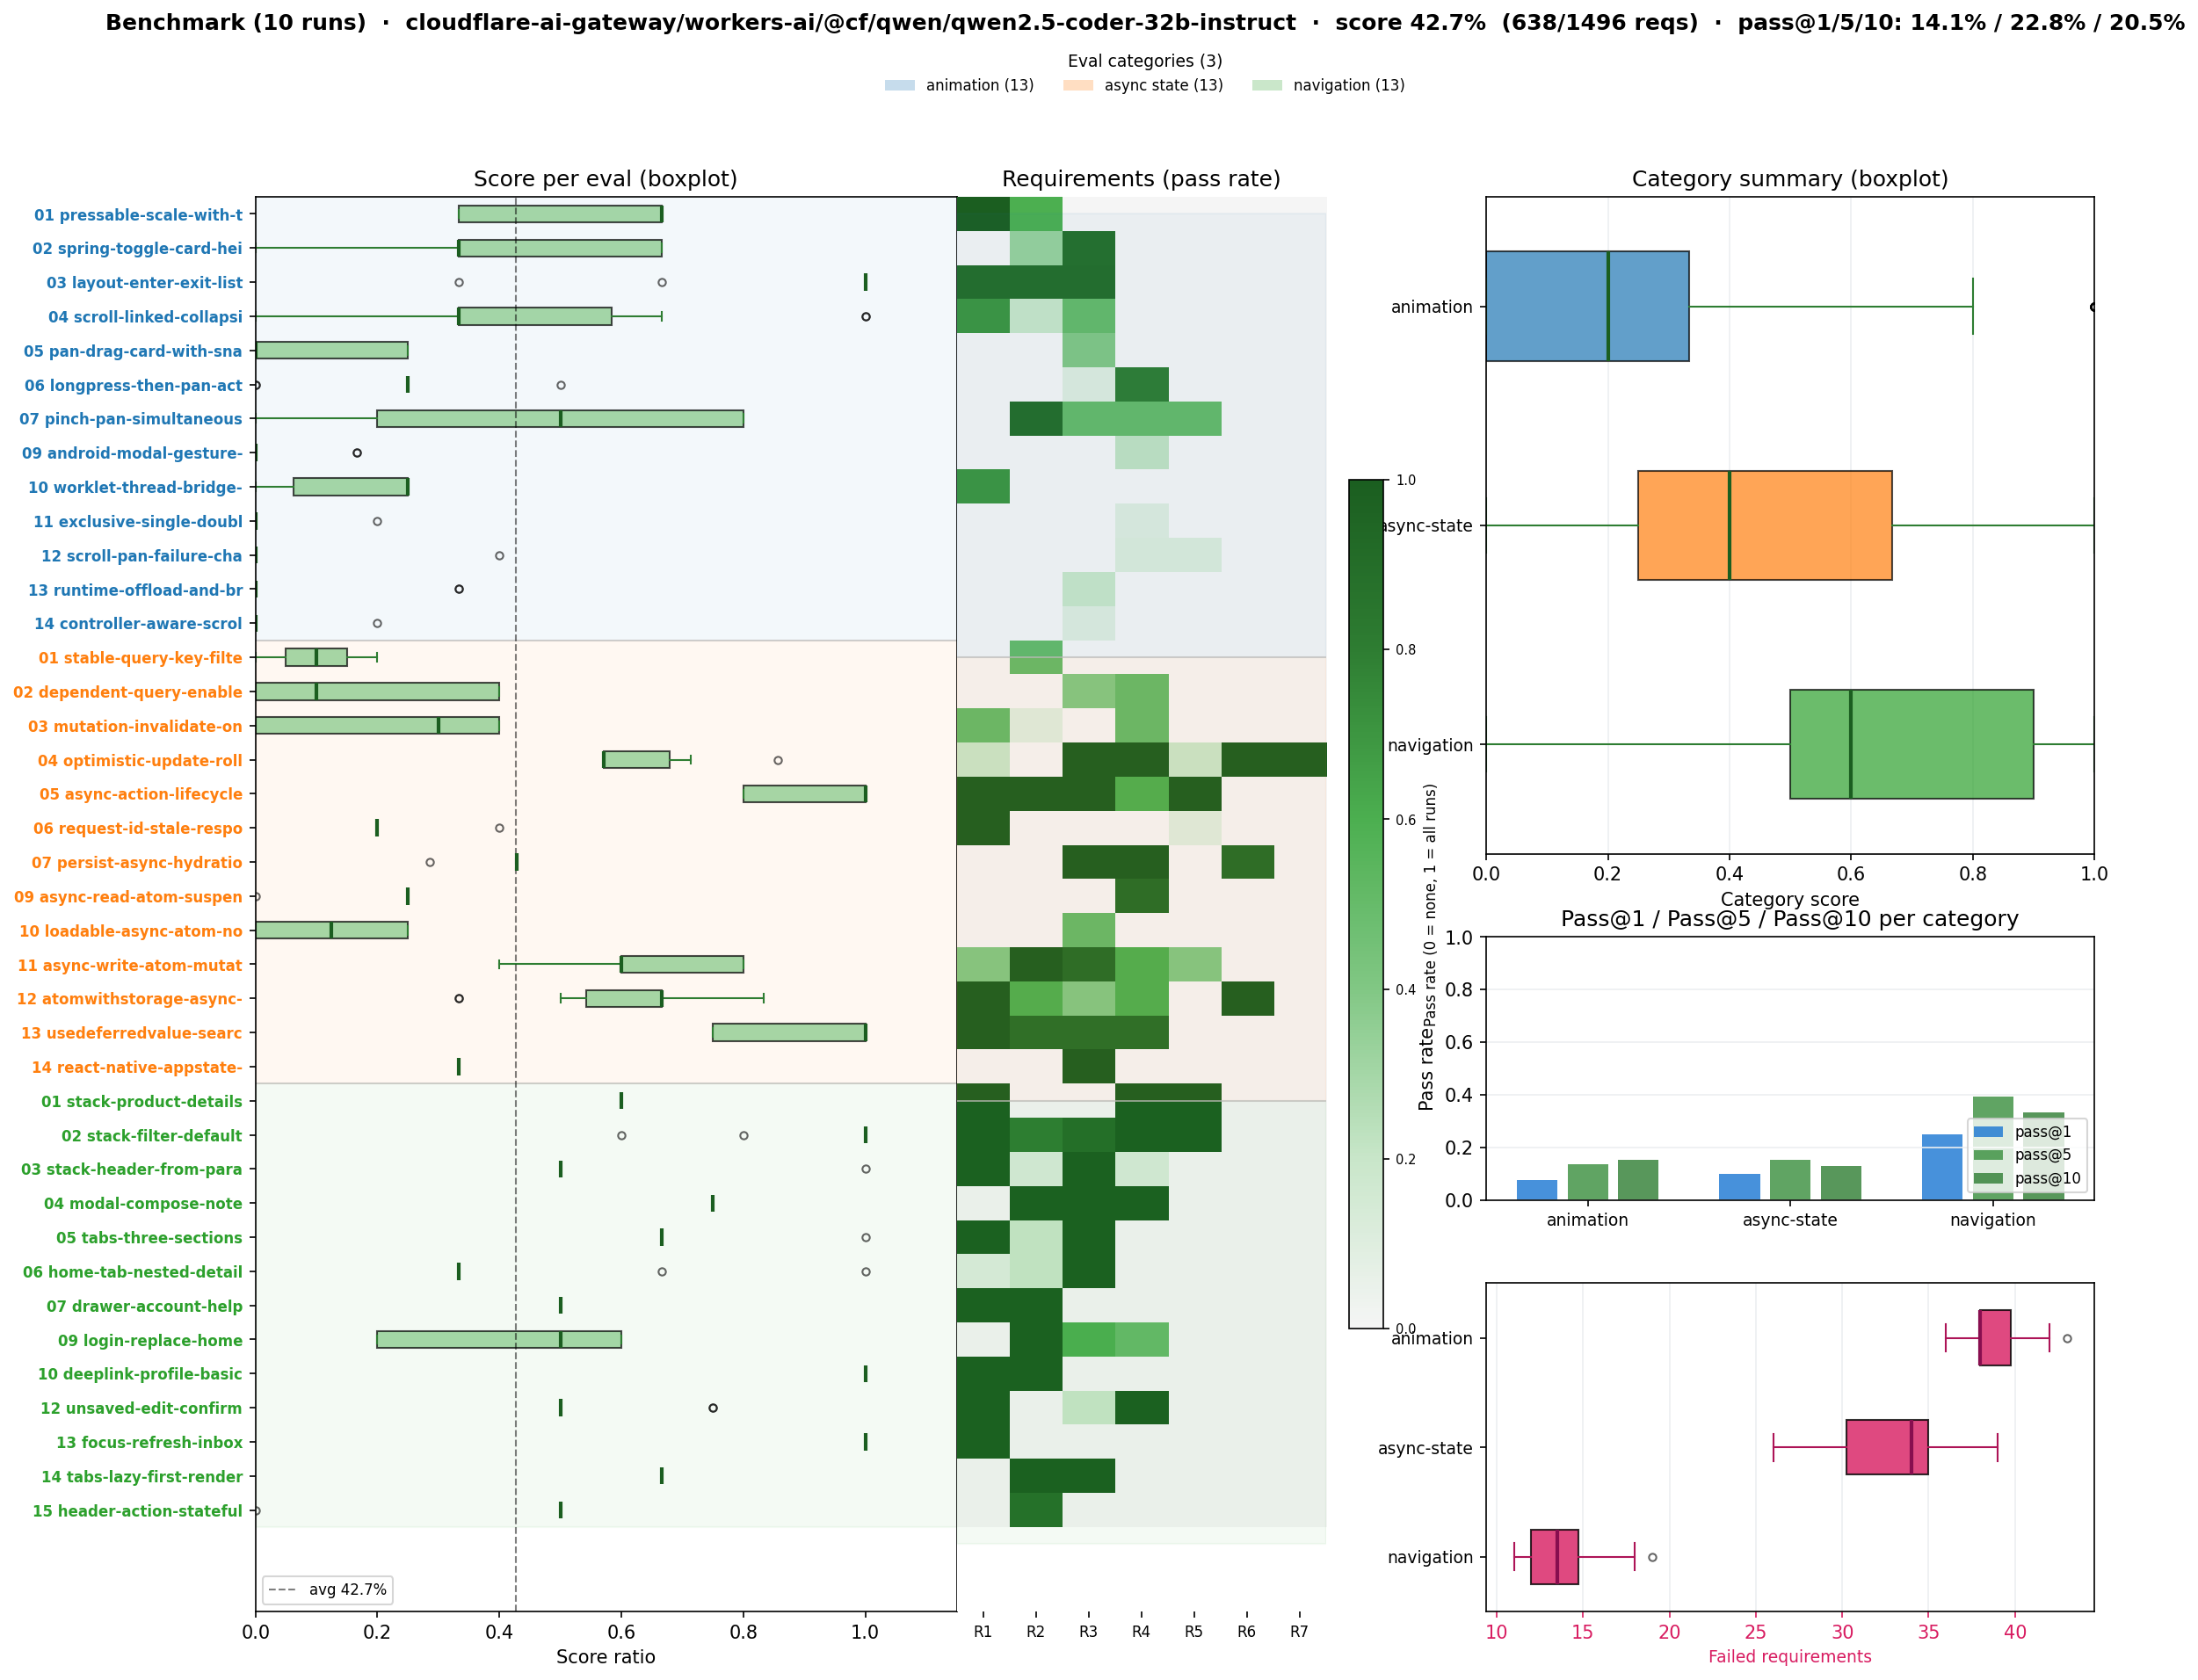
\includegraphics[width=\textwidth]{export/figures/qwen2.5-coder-32b-instruct_benchmark_plot.png}
\caption{Benchmark Plot for qwen2.5-coder-32b-instruct.}
\end{figure}

\begin{figure}[htbp]
\centering
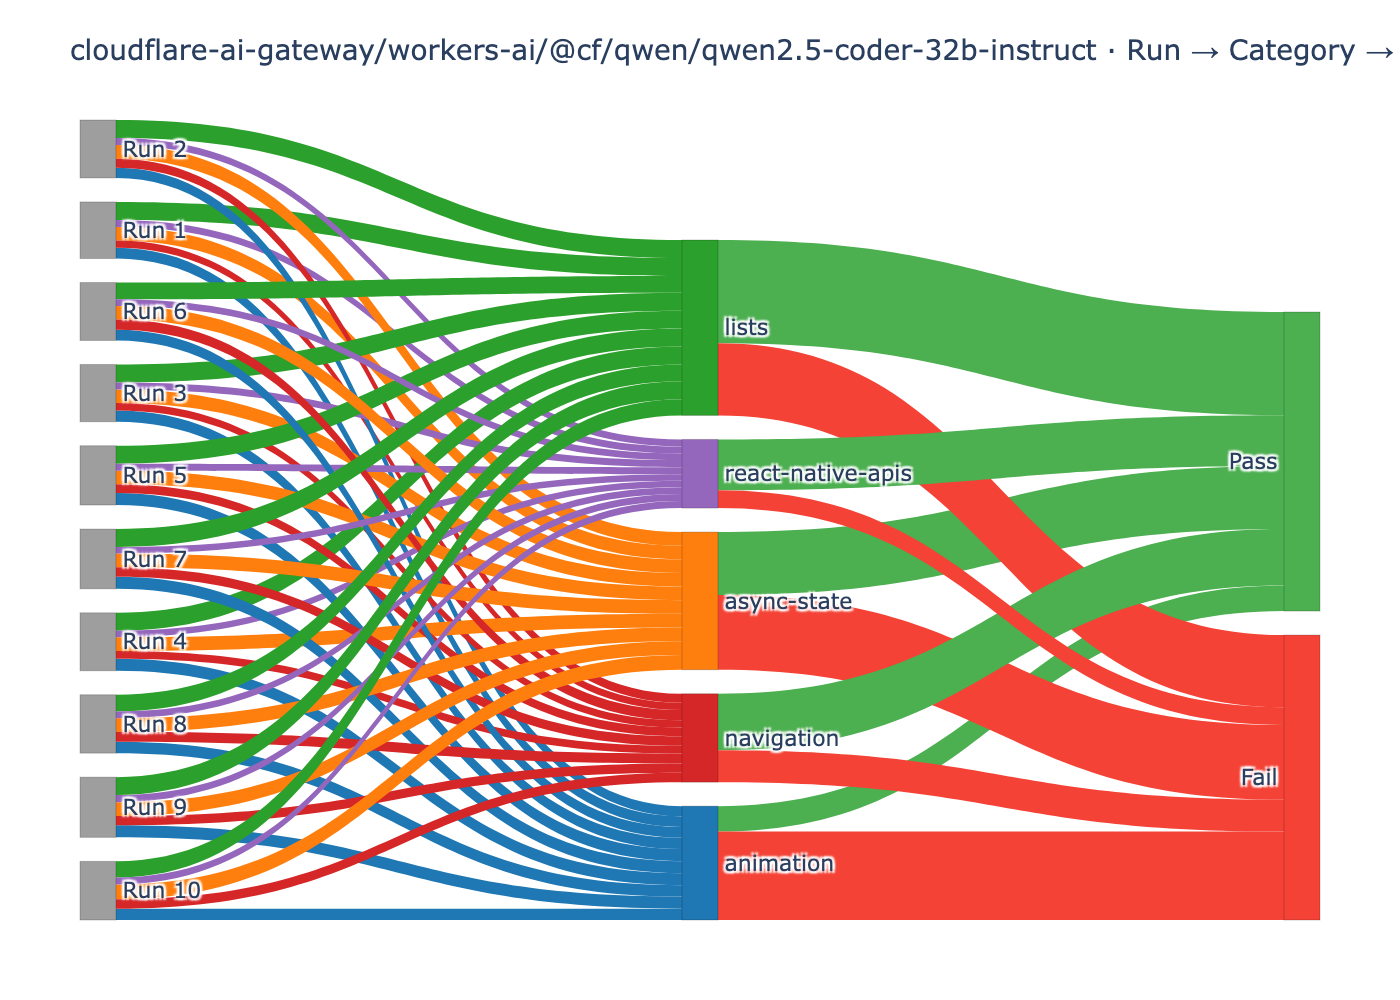
\includegraphics[width=\textwidth]{export/figures/qwen2.5-coder-32b-instruct_sankey_per_run.png}
\caption{Sankey per run for qwen2.5-coder-32b-instruct showing the distribution of evals with respect to categories and results}
\end{figure}


\end{document}
